\documentclass{dissertation}

\usepackage[version=4]{mhchem}
\usepackage{siunitx}
\usepackage{listings}
\usepackage{pdflscape}
\usepackage{enumitem}
\usepackage{amsmath}
\usepackage{amssymb}
\usepackage[final]{pdfpages}
\usepackage{booktabs}
\usepackage{longtable}
\usepackage{rotating}
\usepackage{makecell}
\usepackage{makecell}
\usepackage{multirow}
\usepackage{setspace}
\usepackage{nameref}
\usepackage{caption}
\usepackage{subcaption}
\usepackage[acronym]{glossaries}
\usepackage{float}
\usepackage[justification=centering]{caption}
\makeglossaries

\theoremstyle{definition}
\newtheorem*{objective}{Objective}
 
\theoremstyle{remark}
\newtheorem*{constraint}{Constraints}

\newcommand{\ra}[1]{\renewcommand{\arraystretch}{#1}}

\newcommand{\compresslist}{
	\setlength{\itemsep}{1pt}
	\setlength{\parskip}{0pt}
	\setlength{\parsep}{0pt}
	}
\onehalfspacing

\renewcommand*{\lstlistlistingname}{List of Listings}

\begin{document}

%% Specify the title and author of the thesis. This information will be used on
%% the title page (in title/title.tex) and in the metadata of the final PDF.\documentclass{dissertation}

% Format: \title[Optional Subtitle]{Title}
\title{Coupled Radiation Transport and Mobile Depletion for Health Physics and Environmental Impact Applications} 
\author{Kevin}{Sawatzky}

%% Use Roman numerals for the page numbers of the title pages and table of
%% contents.
\frontmatter

\doublespacing
\begin{titlepage}

%\begin{center}
%
%
%%% Extra whitespace at the top.
%\vspace*{2\bigskipamount}
%
%%% Print the title.
%{\makeatletter
%\CoverFont{b}{18}{20pt}\LARGE\@title
%\makeatother}
%
%%% Print the optional subtitle.
%{\makeatletter
%\ifx\@subtitle\undefined\else
%    \bigskip
%    \titlefont\titleshape\Large\@subtitle
%\fi
%\makeatother}
%
%\end{center}
%
%\cleardoublepage
\thispagestyle{empty}

\begin{center}

%% The following lines repeat the previous page exactly.

\vspace*{2\bigskipamount}

%% Print the title.
{\makeatletter
\CoverFont{b}{18}{20pt}\LARGE\@title
\makeatother}

%% Print the optional subtitle.
{\makeatletter
\ifx\@subtitle\undefined\else
    \bigskip
    \CoverFont{m}{12}{14pt}\Large\@subtitle
\fi
\makeatother}

%% Uncomment the following lines to insert a vertically centered picture into
%% the title page.
%\vfill
%\includegraphics{title}

%% Apart from the names and dates, the following text is dictated by the
%% promotieregelement.

\bigskip
\bigskip
\bigskip
\bigskip
\bigskip
\bigskip

by

\bigskip
\bigskip

%% Print the full name of the author.
\makeatletter
{\bf \@firstname\ {\@lastname}}
\makeatother

\bigskip
\bigskip
\bigskip
\bigskip

A thesis submitted to the\\
School of Graduate and Postdoctoral Studies\\
in partial fulfilment of the requirements for the degree of 

\bigskip
\bigskip
\bigskip
\bigskip

{\bf{Masters of Applied Science}}

% \medskip

in

%  \medskip

{\bf{Nuclear Engineering}}

\bigskip
\bigskip
\bigskip
\bigskip

Department of Energy and Nuclear Engineering, Faculty of Engineering and Applied Science

\medskip

University of Ontario Institute of Technology (Ontario Tech University)

\medskip

Oshawa, Ontario, Canada

\medskip

April 2024

\vfill


\bigskip
\textcopyright{} \makeatletter \@firstname\ {\@lastname}\makeatother, 2024


%\date{\today}

%% Extra whitespace at the bottom.
\vspace*{2\bigskipamount}

\end{center}

\end{titlepage}

\setcounter{page}{2}
\cleardoublepage
\thispagestyle{plain}
\addcontentsline{toc}{chapter}{Thesis Examination Information}

%% The following line is dictated by the promotieregelement.
\begin{center}
\textbf{THESIS EXAMINATION INFORMATION}

\bigskip

Submitted by:  \makeatletter\textbf{\@firstname\ {\@lastname}}\makeatother

\bigskip
\bigskip

\textbf{Masters of Applied Science} in \textbf{Nuclear Engineering}

\end{center}


\bigskip
\bigskip

\noindent \fbox{
    \parbox{\textwidth}{Thesis title: \makeatletter {Coupled Radiation Transport and Mobile Depletion for Health Physics and Environmental Impact Applications} \makeatother}
}

\bigskip

An oral defense of this thesis took place on April 10\textsuperscript{th} 2024 in front of the following examination committee:

\medskip

\noindent\textbf{Examining Committee:}

\bigskip

\begingroup
\renewcommand{\arraystretch}{2}
\begin{tabular}{lcl}
    Chair of Examining Committee &\phantom{Alphabet} & Prof. Akira Tokuhiro \\
    Research Supervisor && Prof. Kirk D. Atkinson\\
    Examining Committee Member && Prof. Markus H.A. Piro \\
    Thesis Examiner && \makecell[l]{ Dr. Mark DeHart \\ Idaho National Laboratory (USA) }\\
\end{tabular}
\endgroup

\bigskip

\noindent The above committee determined that the thesis is acceptable in form and content and that a satisfactory knowledge of the field covered by the thesis was demonstrated by the candidate during an oral examination. A signed copy of the Certificate of Approval is available from the School of Graduate and Postdoctoral Studies.
%% The (optional) dedication can be used to thank someone or display a
%% significant quotation.
% \dedication{\epigraph{This perpetual motion machine she made today is a joke, it just keeps going faster and faster... \\ Lisa ... In this house, we OBEY the laws of thermodynamics!}{Homer Simpson}}
\chapter*{Abstract}
\addcontentsline{toc}{chapter}{Abstract}
\setheader{Abstract}

The next generation of nuclear reactors pose a large challenge to existing computational methods. \texttt{Caribou} is a MOOSE-based health physics and environmental impact code under development at Ontario Tech which aims to address some of these challenges. This work developed a discrete ordinates radiation transport solver and a radionuclide trace species transport solver in the MOOSE framework for \texttt{Caribou}. This radiation transport solver is compared to several benchmark problems to determine its accuracy with and without ray effect mitigation measures, finding good agreement with all the problems tested. The trace species transport solver is then verified with the method of manufactured solutions. The coupled solvers are then used to analyze the formation of $\mathrm{^{41}Ar}$ in a containment volume due to ex-core neutron fields, and the photon fields from a $\mathrm{^{137}Cs}$ plume. The conclusions of this work indicate that these methods are a valuable addition to \texttt{Caribou}'s suite of capabilities.

\bigskip
\bigskip
\bigskip
\bigskip

\noindent \textbf{Keywords:} Ex-Core Radiation Transport; Mobile Depletion; Discrete Ordinates; MOOSE; \texttt{Caribou}
\chapter*{Author's Declaration}
\addcontentsline{toc}{chapter}{Author's Declaration}
\setheader{Author's Declaration}

I hereby declare that this thesis consists of original work of which I have authored. This is a true copy of the thesis, including any required final revisions, as accepted by my examiners.

I authorize the University of Ontario Institute of Technology (Ontario Tech University) to lend this thesis to other institutions or individuals for the purpose of scholarly research. I further authorize University of Ontario Institute of Technology (Ontario Tech University) to reproduce this thesis by photocopying or by other means, in total or in part, at the request of other institutions or individuals for the purpose of scholarly research. I understand that my thesis will be made electronically available to the public.

\bigskip
\bigskip

\makeatletter\textbf{\@firstname\ {\@lastname}}\makeatother
\chapter*{Statement of Contributions}
\addcontentsline{toc}{chapter}{Statement of Contributions}
\setheader{Statement of Contributions}

I hereby certify that I am the sole author of this thesis. I have used standard referencing practices to acknowledge ideas, research techniques, or other materials that belong to others. Furthermore, I certify that I am the sole source of the creative works and/or inventive knowledge described in this thesis. The work presented in this thesis which has been published, or is in the process of being published, can be found below.

\noindent\textbf{First Collision Source}

The Self-Adjoint Scalar Flux first-collision source discussed in Section~\ref{solver:radiation_transport:sasf_point_source} will be submitted for publication in the Journal of Computational Physics. The author of this thesis was responsible for conceptualising the work, performing mathematical derivations, devising computational testing, generating results, and writing the manuscript. K.D. Atkinson revised the manuscript.

\noindent\textbf{Verification with the Proposed OTU Subcritical Assembly Facility}

A portion of the verification studies presented in Section~\ref{verification:radiation_transport_sn:subcritical} involving the proposed Ontario Tech subcritical assembly have been published as: \textbf{K.\ Sawatzky} and {K.\ D.\ Atkinson}, \textit{Verification of a CARIBOU-OpenMC Workflow for the Analysis of HTGR-Like Systems Using the Proposed Ontario Tech Subcritical Assembly}, \href{https://www.ans.org/meetings/physor2024/}{Proceedings of PHYSOR-2024, (San Francisco, California, USA), American Nuclear Society, 2024}. The author of this thesis was responsible for conceptualising the work, devising computational testing, generating results, and writing the manuscript. K.D. Atkinson revised the manuscript.
\chapter*{Acknowledgements}
\addcontentsline{toc}{chapter}{Acknowledgements}
\setheader{Acknowledgements}
\label{acknowledgements}

I would like begin by thanking my supervisor Prof. Kirk Atkinson for the significant impact he has had on my career, professional development, and my research interests. From hiring me as a research student over the summer of 2020, to supervising my capstone project in the final year of my undergraduate studies, and agreeing to take me on as a graduate student with a project that I had the ability to shape to my own interests; you have always supported me as I grew into academia. Even though you have been incredibly busy as of late, you've always taken the time to chat, provide feedback on my work, and encourage me to explore areas I'm interested in which are only tangentially related to my research project. I cannot thank you enough for everything you've done for me over the last four years.

I would like to acknowledge several other faculty members at Ontario Tech for providing guidance and support over the last few years. I would like to start with Prof. Markus Piro, thank you for agreeing to be on my supervisory committee. I appreciate how you've always made time to talk and provide advice regarding my work or career as a whole. Prof. John Froats, thank you for your mentorship through several teaching assistant positions. You've taught me what it means to be a nuclear professional. Prof. Rachid Machrafi, thank you for encouraging me to consider graduate studies. Without your advice, I would not be here today. 

Though it would be impossible to name them all, I wish to thank the many colleagues that I've met through my time here at Ontario Tech. To Amna Hassan, Scott McKay and Viridiana Borjas Padilla, thank you for listening to my rants and in general being the best lab mates one could want. I want to thank Daniel Chen, Graeme Francolini, Morgan Collins, Nicholas Somer, Nikolas Lymberis Scuro, and Tyra Gordon. I appreciate all of our conversations about both work and life, the many lunches and coffee breaks, and in general making graduate school at Ontario Tech a positive experience. We may have started out as colleagues, but I am proud to call you all my friends.

Lastly, I would like to thank my family and close friends for always being there for me. In particular, I want to thank my mother Aganetha, my father Cornelio, and my brother Alexander for pushing me to continue higher education and pursue my passions. To my good friends Adam, Charlie, Ethan, Luka, Nam, Nathan and Tommy, thank you for your patience whenever I waxed on about my research completely unsolicited. 

This research was undertaken thanks to funding provided by the University Network of Excellence in Nuclear Engineering (UNENE) and the Natural Sciences and Engineering Research Council of Canada (NSERC) through the Industrial Research Chairs program [funding reference number IRCPJ 549979-19]. 
\tableofcontents
\listoffigures
\listoftables
\addcontentsline{toc}{chapter}{List of Listings}
\lstlistoflistings
\newacronym{msr}{MSR}{Molten Salt Reactor}
\newacronym{htgr}{HTGR}{High Temperature Gas-cooled Reactor}
\newacronym{lwrs}{LWRs}{Light Water Reactors}
\newacronym{pthwrs}{PTHWRs}{Pressure Tube Heavy Water Reactors}
\newacronym{triso}{TRISO}{TRi-structural ISOtropic}
\newacronym{smrs}{SMRs}{Small Modular Reactors}
\newacronym{cnsc}{CNSC}{Canadian Nuclear Safety Commission}
\newacronym{iaea}{IAEA}{International Atomic Energy Agency}
\newacronym{gnat}{Gnat}{General Neutral particle Analysis Toolkit}
\newacronym{moose}{MOOSE}{Multiphysics Object Oriented Simulation Environment}
\newacronym{petsc}{PETSc}{Portable Extensible Toolkit for Scientific Computation}
\newacronym{ad}{AD}{Automatic Differentiation}
\newacronym{inl}{INL}{Idaho National Laboratory}
\newacronym{cfd}{CFD}{Computational Fluid Dynamics}
\newacronym{sn}{S\textsubscript{N}}{Discrete Ordinates}
\newacronym{pn}{P\textsubscript{N}}{Spherical Harmonics}
\newacronym{moc}{MOC}{Method of Characteristics}
\newacronym{fvm}{FVM}{Finite Volume Method}
\newacronym{dgfem}{DGFEM}{Discontinuous Galerkin Finite Element Method}
\newacronym{cgfem}{CGFEM}{Continuous Galerkin Finite Element Method}
\newacronym{saaf}{SAAF}{Self Adjoint Angular Flux}
\newacronym{supg}{SUPG}{Streamline-Upwind Petrov Galerkin}
\newacronym{sasf}{SASF}{Self-Adjoint Scalar Flux}
\newacronym{xml}{XML}{Extensible Markup Language}
\newacronym{pjfnk}{PJFNK}{Preconditioned Jacobian-Free Newton Krylov}
\newacronym{gmres}{GMRES}{Generalized Minimal Residual Method}
\newacronym{mms}{MMS}{Method of Manufactured Solutions}
\newacronym{bwr}{BWR}{Boiling Water Reactor}
\newacronym{iter}{ITER}{International Thermonuclear Experimental Reactor}

\singlespacing

\printglossary[type=\acronymtype,nonumberlist]
\addcontentsline{toc}{chapter}{Acronyms}
\setheader{Acronyms}


%\onehalfspacing
\doublespacing
% \include{preface/preface}
% \include{summary/summary}

%% Use Arabic numerals for the page numbers of the chapters.
\mainmatter

%% Turn on thumb indices.
%\thumbtrue

\chapter{Introduction} 
\label{introduction}

Climate change has long been viewed as one of the greatest challenges of the modern era, with governments around the world implementing policies designed to encourage heavy industries and the electrical grid to reduce greenhouse gas emissions. Nuclear energy is anticipated to play a major role in this new low-carbon economy, resulting in an expansion of nuclear generating capacity world-wide. Many reactor vendors are proposing that this expansion be conducted with novel Generation IV reactor designs that have advantages over \acrfull{lwrs} and \acrfull{pthwrs}; some of these advantages include low pressure operation, the use of advanced fuels such as \acrfull{triso} fuel, and high thermal efficiencies \cite{gen_iv_2022_annual_report}. A sample of these technologies include the \acrfull{msr} and \acrfull{htgr}. This next generation nuclear fleet may also adopt \acrfull{smrs} due to their various advantages when compared to conventional facilities, which include a reduced physical footprint, smaller core radionuclide inventories, reduced reactor powers, and decreased plant costs \cite{iaea_2021_fast_reactors, nea_2021_smr_opportunities_challenges}. These new reactor technologies pose many challenges when compared to existing reactors, where the most prominent challenge is a lack of reactor operating experience \cite{iaea_2022_lessons_learned}. Advances in high-performance computing have allowed modelling and simulation to augment the limited existing operational experience and guide further experiments, motivating the development of high-fidelity multiphysics methods for the design and analysis of nuclear systems. 

The main motivation behind the development of new codes is the design of advanced reactors; however, the analysis of these new reactors for the purposes of safety and determining their environmental impact is also of importance. The aim of this work is to develop a series of high-fidelity methods useful for health physics and environmental impact applications, filling a gap that exists for safety analysis. This chapter aims to provide context to the need for these methods, starting with a discussion of health physics concerns posed by the development of advanced reactors. This is followed by a description of the \acrfull{moose} and \texttt{Caribou}, a health physics and environmental impact code built on \acrshort{moose} which this work contributes to.

\section{Health Physics Concerns in Advanced Reactors}
\label{introduction:hp_advanced}

Nuclear safety analysis and environmental impact assessments verify that a nuclear plant meets the high-level safety goals of the regulator (i.e. a maximum allowed radiation dose) prior to construction or modification \cite{regdoc_2_4_1, regdoc_2_5_2}; a necessary step along the path to deployment which is required by national regulatory bodies such as the \acrfull{cnsc}. The technological benefits of Generation IV reactors and \acrshort{smrs} have resulted in several licensing challenges with regards to environmental impact and nuclear safety. \acrshort{triso} fuels are layered such that the fuel itself acts as a series of containment boundaries \cite{triso_ref_piro}, and so \acrshort{htgr} reactor vendors are proposing that these designs do not need separate containment structures and exclusion zones \cite{iaea_2022_lessons_learned}. Removing the containment structure and exclusion zone places additional scrutiny on existing reactor components and system boundaries, motivating the use of analysis methods which reduce uncertainty in high-level safety metrics. \acrshort{msr}s use a liquid fuel salt as opposed to traditional solid fuel assemblies. The piping required to move fuel from the reactor vessel to a primary heat exchangers results in long radiation streaming paths, complicating the design of shielding and presenting another radiation hazard. Many of these novel reactors operate with a different neutron spectrum and a higher fuel enrichment, resulting in ex-core\footnote{Recent advances in reactor multi-physics methods have addressed in-core nuclide inventories for Generation IV reactors, and so the focus of this work is on ex-core radionuclide sources.} radionuclide inventories which differ from the current fleet of \acrshort{lwrs} and \acrshort{pthwrs}. \acrshort{smrs} have higher leakage fractions then conventional power reactors. This couples with smaller containment systems, which may result in an increased formation of mobile effluents along with higher structural material activation rates per unit of reactor power. These transmutation products pose a challenge to analysis methods which use empirical correlations as these simplified methods have largely been derived for \acrshort{lwrs} and \acrshort{pthwrs}.

New computational tools can assist in mitigating the previously discussed health physics concerns inherent to novel reactor technologies. Neutral particle transport and nuclide dispersion are two phenomena that require modelling for safety analyses, environmental impact assessments, operational work planning, and the design of shielding. Simulating the behavior of neutrons and gamma photons emitted by a nuclear reactor into the containment system yields insight into the evolution of radionuclide inventories, while also providing direct radiation fields useful for determining radiation dose rates and the design of the reactor biological shield. The simulation of secondary gamma photon fields generated by the decay of these in-containment radiation source terms also proves to be invaluable for outage work planning and the selection of portable photon shielding used to perform maintenance tasks. Modelling radionuclide dispersion becomes necessary when evaluating the environmental impact of highly mobile radionuclide effluents (e.g., $\mathrm{^{3}H}$, $\mathrm{^{14}C}$, and $\mathrm{^{41}Ar}$) formed during normal operations, and the dose consequences caused by the controlled release of core materials during an accident sequence. In the latter case nuclides of importance to accident analysis such as $\mathrm{^{137}Cs}$ \cite{regdoc_2_5_2} have decay chains which include isomeric transitions, resulting in photon emissions in the form of gamma radiation. This necessitates the use of photon transport to calculate the external dose from the emission, and dispersion methods to compute the evolution of the spatial distribution of nuclides over time. Finally, high-fidelity methods can reduce uncertainties in radiation dose predictions to support the case for removing containment structures and shrinking exclusion zones. 

\section{Multi-Physics Simulations for Health Physics Applications}
\label{introduction:ms}

Previous methods for evaluating the environmental impact of nuclear facilities were largely confined to low-fidelity atmospheric and aqueous dispersion methods using experimentally determined dispersion coefficients, coupled with simplified analytical solutions for radiation fields produced by the plume for computing external radiation doses \cite{nf_rdd_trials_i,nf_rdd_trials_ii,n_288_1_20,n_288_2_19}. The concentration of highly mobile radionuclide effluents are computed using simplified neutron flux models and transfer functions to account for the movement of radionuclides between different control volumes, such as the containment building to the atmosphere \cite{ar41_triga_1,n_288_1_20}. Recent developments in computational methods and high performance computing allow for the use of multi-scale, multiphysics methods to enable the modelling of physical phenomena which was previously ignored to err on the side of conservatism. This reduces the uncertainty in calculations used to support the licensing of facilities and aids in guiding experimental work required for site and reactor characterisation.

\begin{figure}[H]
    \centering
    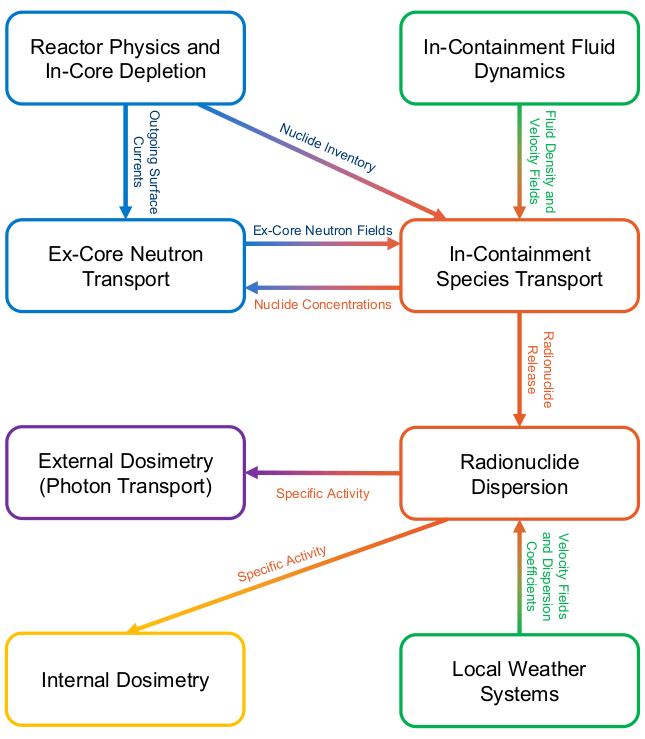
\includegraphics[width=0.65\textwidth]{images/introduction/release_multiphysics.png}
    \caption{Multiphysics phenomena in an airborne release of radioactive material.}
    \label{fig:introduction:ms:physics}
\end{figure}

The formation of nuclides in ex-core radiation fields, the transport of nuclides, and the resulting dosimetry concerns span many different physics and cover several different length scales. As an example, consider the various phenomena involved in an airborne radioactive release from a reactor containment building (Figure~\ref{fig:introduction:ms:physics}). Neutron transport within the containment building takes place over length scales of centimeters to metres and times scales of nanoseconds to microseconds. The formation and transport of effluents within containment is governed by the resulting neutron fields and airflow within containment, with length scales from metres to tens of metres and time scales on the order of seconds to minutes. The atmospheric dispersion of releases takes place over length scales of hundreds of metres to kilometres and time scales of hours to days. This is dependant on local weather patterns, the complexities of the terrain surrounding the nuclear facility, and the local built environment. Finally, external photon dosimetry is concerned with length scales that range from metres to hundreds of metres (depending on the activity of the release) and time scales on the order of nanoseconds to milliseconds. It is clear that a multiphysics approach which considers these differences in length and time scales are required for modern computational methods used to evaluate the environmental impact of nuclear facilities.

\subsection{The Multiphysics Object Oriented Simulation Environment}
\label{introduction:ms:moose}

The need to move towards a multiphysics and multi-scale approach for analysis of many nuclear systems resulted in the development of the \acrshort{moose}, an open-source simulation framework designed to take advantage of recent advances in massively parallel computing to solve larges systems of partial differential equations \cite{moose_0,moose_1,moose_2}. \acrshort{moose} was initially developed at \acrfull{inl} with the main aim of abstracting the more complicated tasks that are required to develop a new analysis code, such as the machinery of numerical discretization and the sparse linear algebra required to solve the resulting system of nonlinear equations. To enable this functionality, \acrshort{moose} wraps the \acrfull{petsc} \cite{petsc_manual} for state of the art sparse matrix solution algorithms and libMesh \cite{libmesh} for finite element and finite volume discretization schemes. \acrshort{moose} provides many other features which make it more suitable for multiphysics calculations than competing frameworks. These include \acrfull{ad} \cite{moose_ad}, automatic documentation and quality assurance to NQA-1 \cite{moose_civet}, in memory coupling between different \acrshort{moose} applications \cite{moose_coupling}, and a plethora of common physics modules \cite{moose_ns_summary,moose_th,moose_reactor}. Of particular importance to this work is the \texttt{NavierStokes} module \cite{moose_ns_summary,moose_ns_crab}, which includes capabilities used by the coarse-mesh thermal-hydraulics code \texttt{Pronghorn} developed at \acrshort{inl}.

There are many \acrshort{moose}-based applications (both open-source and export controlled) which have been developed for modelling nuclear reactors and other nuclear systems. These include export controlled codes such as \texttt{Griffin} \cite{griffin_sdp} for in-core radiation transport and nuclide depletion, \texttt{Pronghorn} \cite{moose_ns_crab} for coarse-mesh computational fluid dynamics, and \texttt{Yellowjacket} \cite{yellowjacket} for corrosion and fuel chemistry. Open-source applications include \texttt{Moltres} \cite{moltres} for the simulation of coupled \acrshort{msr} neutron diffusion and thermal-hydraulics, and \texttt{Cardinal} \cite{cardinal} for high-fidelity multiphysics simulations using Monte Carlo radiation transport (through \texttt{OpenMC} \cite{openmc}) and spectral elements \acrfull{cfd} (using \texttt{NekRS}). 

While the \acrshort{moose} ecosystem contains many applications with wide ranging capabilities it still lacks a dedicated tool for performing health physics and environmental impact analysis. The reactor physics applications \texttt{Griffin} and \texttt{Cardinal} can be used to fill some of the requirement of a health physics code, namely external dosimetry and ex-core neutron transport. However, there are several disadvantages to taking this approach. The use of \texttt{Griffin} would necessitate that any capabilities added to facilitate health physics analysis be placed under export control. The use of \texttt{Cardinal} for long length scale radiation transport problems such as  ex-core activation and shielding analysis is largely impractical due to the lack of deterministic variance reduction techniques, yielding increasingly large uncertainties in tallies as one moves away from the reactor core or radionuclide sources. The \texttt{NavierStokes} module can solve for radionuclide distributions within fluids over short length scales, such as in fission reactor cores and containment systems. However, there is no capability built in \acrshort{moose} to integrate either aqueous or atmospheric dispersion of radioactive releases with meso scale weather models over length scales of kilometers. To address this gap in capabilities a new multiphysics health physics and environmental impact code named \texttt{Caribou} is under development at Ontario Tech\footnote{The development of \texttt{Caribou} if being performed independently without any collaborations with \acrshort{inl}.}. The work performed in this thesis contributes to this new code, adding a near-field radiation transport and trace species transport solver to \texttt{Caribou}. Its relationship to, and a description of \texttt{Caribou} are described in the following section.

\subsection{Caribou}
\label{introduction:ms:caribou}

As a response to the health physics and environmental challenges posed by Generation IV reactors and \acrshort{smrs}, \texttt{Caribou} is designed to enable predictive modelling of static and transient radiological events within a multiphysics and multi-scale framework. \texttt{Caribou} has two main objectives: to reduce uncertainties across various length scales, and to provide high quality reference data to more accurately predict radiological consequences after a nuclear accident. As shown in Figure~\ref{fig:introduction:ms:caribou:caribou}, \texttt{Caribou} will contain capabilities for neutral particle transport, radionuclide species transport, and \acrshort{cfd}. The methods required to simulate species transport change depending on the fluid the radionuclides are suspended in and the length scale under consideration. \texttt{Caribou} handles this difficulty by first differentiating species transport by length scale, where near-field transport occurs at lengths of tens to hundreds of meters and far-field transport occurs at distances greater than one kilometer. The far-field species transport is then further separated into atmospheric dispersion and aqueous dispersion owing to the differences in underlying fluid and weather modelling required to simulate species transport in those cases. The development of the far-field dispersion capabilities along with coupling these capabilities to meso scale weather models are the subjects of additional research efforts at Ontario Tech, while this work focuses on near-field radiation transport and trace species transport.

\begin{figure}[H]
    \centering
    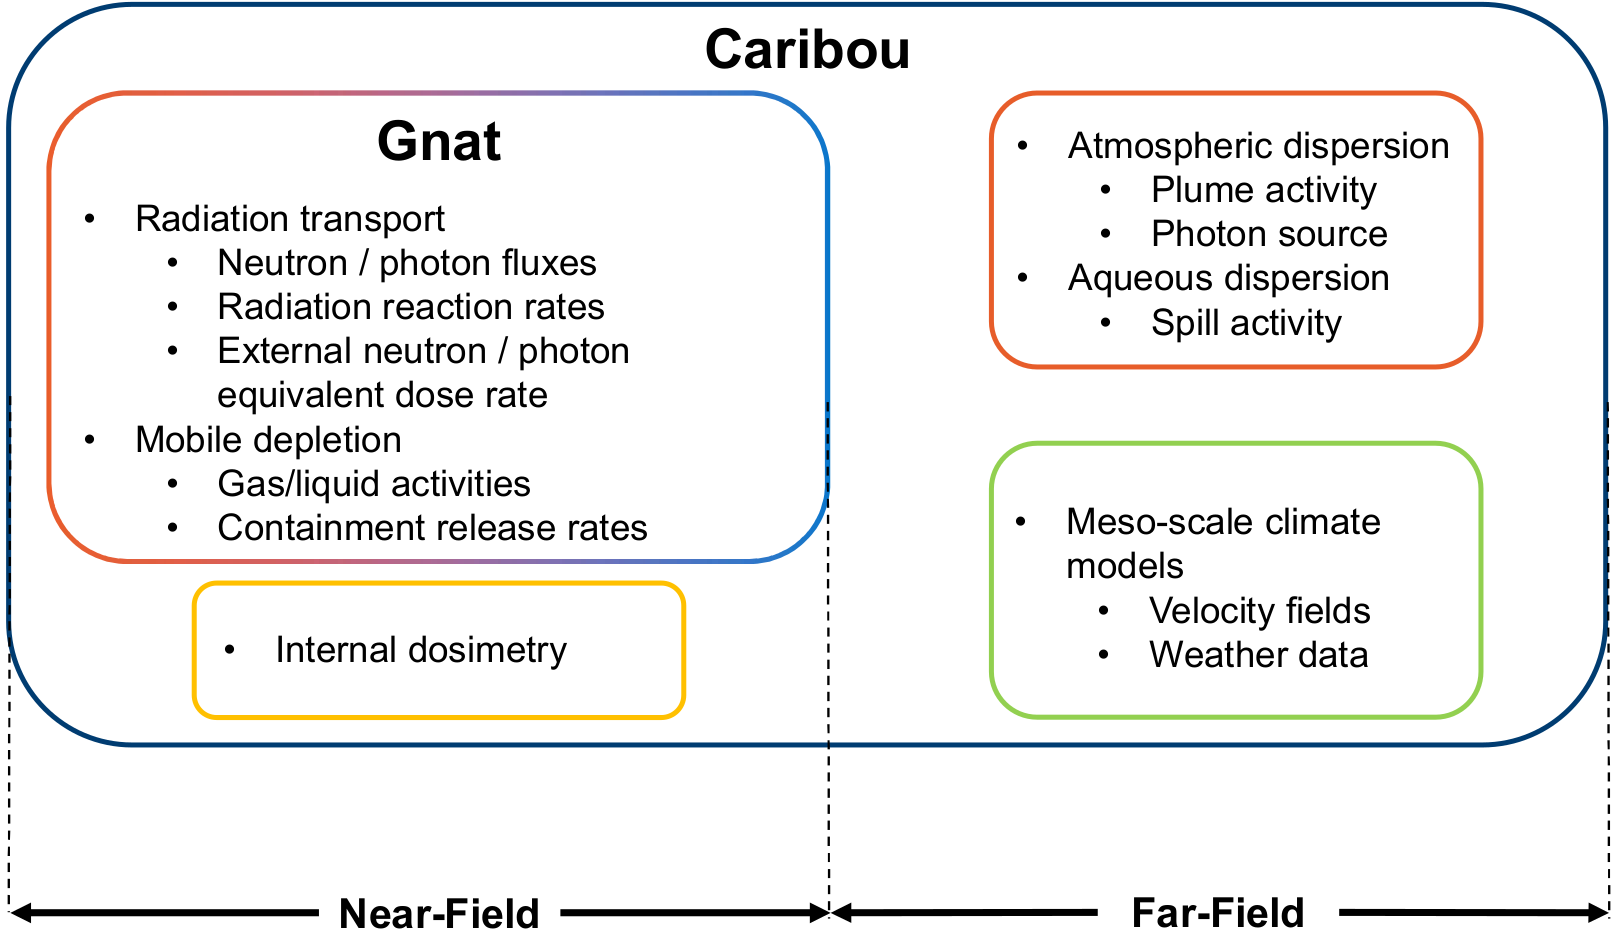
\includegraphics[width=1.0\textwidth]{images/introduction/caribou.png}
    \caption{Current and planned capabilities of \texttt{Caribou}.}
    \label{fig:introduction:ms:caribou:caribou}
\end{figure}

Near-field capabilities, such as radiation transport and the transport of radioactive trace species, are valuable capabilities for \texttt{Caribou} to have. Neutron transport within containment systems allow analysts to compute ex-core nuclide source terms, which may be released during a nuclear accident. Coupling neutron transport with trace species transport allows for the computation of gaseous / liquid source terms, such as $\mathrm{^{16}N}$ or $\mathrm{^{41}Ar}$ activities and predicting their behaviour. These potentially novel source terms can be provided to the far-field dispersion models entirely within \texttt{Caribou}, avoiding the need to couple together separate codes. Finally, the far-field dispersion models can propagate nuclide activities to the near-field trace species and gamma photon transport solver, allowing for high-fidelity external dose calculations at length scales of meters. Throughout this work, the transmutation of a fluid in a neutron field is referred to as mobile depletion to emphasize the connection with depletion in reactor cores as both share similar numerical challenges. The main motivation behind this work was to enable direct radiation transport, mobile depletion, and the coupling of both physics together within \texttt{Caribou}. This resulted in a \acrshort{moose} mini-application distributed with \texttt{Caribou} called the \acrfull{gnat}. The objectives, tasks, and deliverables of this work are described in the following chapter.

\section{Thesis Structure}
\label{introduction:ms:structure}

The remainder of this thesis is organized as follows. Chapter~\ref{statement_of_work} presents the objectives of the work and the related research tasks. Chapter~\ref{lit_review} provides a literature review on radiation transport methods, trace species transport methods, and previous approaches used for coupled radiation transport and mobile depletion. Chapter~\ref{solver} provides a description of \acrshort{gnat}, the radiation transport and mobile depletion solver implemented as a part of \texttt{Caribou} through this work. Chapter~\ref{verification} discusses the steps taken to verify the solver and provides verification results. Chapter~\ref{demos} presents a series of demonstration problems which showcase the capabilities of \acrshort{gnat}. The work is concluded in Chapter~\ref{conclusion}, and recommendations for future study are provided in Chapter~\ref{recommendations}.
\chapter{Statement of Work} 
\label{statement_of_work}
\section{Problem Statement}
\label{statement_of_work:ps}

Radiation transport and mobile depletion are key physics to consider when performing analyses related to health physics or environmental impact assessments, especially regarding novel reactor designs that have not been fully characterized, such as Generation IV reactors or \acrshort{smrs}. Despite the growing need for high-fidelity radiation transport and mobile depletion capabilities for predictive modelling of novel source terms and radiation hazards, both the open literature and the open-source capabilities in the \acrshort{moose} ecosystem lack such a tool.
The development of a new radiation transport and mobile depletion code is motivated by specific limitations of these established software packages. The vast majority of radiation transport solvers are standalone tools which do not easily accept dynamic particle sources, which are required for computing the radiation dose from a plume. Many \acrshort{cfd} codes have the capability to compute species transport, a limited set of these codes include radioactive decay and none include all of the capabilities required to model the transmutation of an arbitrary fluid in a neutron field. Finally, existing methods are often not designed for the multi-scale coupling required. Therefore, a new radiation transport and mobile depletion solver must be developed to satisfy the requirements of \texttt{Caribou}.

\section{Statement of Objectives}
\label{statement_of_work:so}
The main objective of this work was to incorporate neutral particle radiation transport and mobile depletion capabilities into the suite of capabilities provided by \texttt{Caribou} through the development of a new \acrshort{moose} mini-application called \acrshort{gnat}, which will be distributed with \texttt{Caribou}. \acrshort{gnat} enables the calculation of both fixed and mobile ex-core nuclide source terms for radionuclide dispersion calculations and external dosimetry from various radiation sources; all within \texttt{Caribou}.

\section{Project Tasks}
\label{statement_of_work:tasks}
To accomplish the objective of the work previously outlined, the project was broken up into several discrete tasks:
\begin{itemize}
    \item Development of a neutral particle transport solver. This includes investigating appropriate discretization strategies for source-driven radiation transport, surveying the literature for open-source radiation transport solvers, and the development of the radiation transport solver. See Section~\ref{lit_review:radiation_transport} for a survey of open-source codes and radiation transport methods. See Section~\ref{solver:radiation_transport} for a description of the implemented radiation transport solver.
    \item Development of a mobile depletion solver. This includes investigating methods for trace species transport, surveying the literature for appropriate discretization schemes, developing the solver, and coupling it with the radiation transport solver. See Section~\ref{lit_review:mass_transport} for a survey of species transport methods. Section~\ref{solver:depletion} contains a description of the mobile depletion solver, and Section~\ref{solver:implementation} discusses use cases for coupled radiation transport and mobile depletion.
    \item Verifying the newly developed solvers using benchmark problems and analytical solutions to the governing equations. See Chapter~\ref{verification} for the results of the verification performed.
    \item Demonstrating the capabilities of the solver through the analysis of several coupled radiation transport and mobile depletion problems. See Chapter~\ref{demos}.
\end{itemize}
\chapter{Literature Review} 
\label{lit_review}

Recent advances in high performance computing have enabled the growth of the methods space in the areas of radiation transport and species transport. Problems which were previously considered to be computationally intractable to nuclear analysts can now be performed with modest computational resources. The goal of this chapter is to provide a survey of the open literature for the methods available to computing radiation transport, mobile depletion, and coupling these two phenomena together. The chapter begins by reviewing the numerical methods and open-source codes available for neutral particle transport with an emphasis placed on methods which are more applicable for computing radiation fields outside of a nuclear reactor core. This is followed by a review of methods used for mobile depletion and trace species transport. Finally, the various strategies that have been used to couple radiation transport and mobile depletion for the analysis of radiological hazards are discussed. Throughout this review, an emphasis is placed on discretization schemes which may be easily implemented in the \acrshort{moose} framework, including: \acrfull{fvm} schemes, \acrfull{dgfem} schemes, and \acrfull{cgfem} schemes.

\section{Neutral Particle Transport Methods for Ex-Core Applications}
\label{lit_review:radiation_transport}

The mathematical machinery required to describe the behavior of particles through a background medium was invented in 1872 by Ludwig Boltzmann and has found uses in various fields, from stellar astrophysics to nuclear reactor design \cite{transport_theory}. The governing equation is known as the Boltzmann transport equation; the solutions to which span three dimensions in space, two dimensions in direction, and one dimension each in energy and time. Owing to the complexity of this seven-dimensional phase space there are few analytical solutions to the transport equation, leading to a diverse array of computational methods to compute numerical solutions for engineering applications. These methods can be lumped into two categories: deterministic methods and stochastic methods. 

Stochastic methods, such as the Monte Carlo method avoid computing solutions to the transport equation directly and instead average the random walks of many individual particles through the problem phase space \cite{computational_methods}. This allows for a continuous treatment of each independent variable and is therefore the preferred approach when accuracy is paramount. The disadvantage of the Monte Carlo method is that many particle histories must be simulated when computing spatially-varying quantities such as particle fluxes, resulting in a substantial performance penalty for a required level of accuracy \cite{computational_methods}. This is further exacerbated in the cases of long particle streaming paths with large angle scattering, secondary particle production, and nuclear transmutations in structural materials. These challenges have largely prevented analog Monte Carlo simulations from being used for deep penetration problems without some form of variance reduction driven by a deterministic transport simulation (e.g. Forward-Weight Consistent Adjoint-Driven Importance Sampling \cite{fw_cadis,variance_reduction_review}) or iterative variance reduction (e.g. the Method of Automatic Generation of Importances by Calculation \cite{magic,variance_reduction_review}). Iterative variance reduction techniques require many iterations to converge spatially distributed quantities \cite{variance_reduction_review}, leading to the preferred use of deterministic transport method driven variance reduction methods or the use of deterministic transport methods over Monte Carlo methods for long length scale problems. 

Deterministic methods require each variable of the phase space be discretized resulting in a decrease in accuracy. When this is acceptable, deterministic methods prove to be advantageous as they require fewer computational resources to compute spatially varying quantities such as reaction rates \cite{applied_reactor_physics}. Individual deterministic transport methods have various advantages and disadvantages depending on the angular discretization scheme employed. This section discusses the major deterministic transport approaches which can be easily implemented in a finite element framework and major open-source radiation transport codes which may be integrated into the \acrshort{moose} framework.

\subsection{The Discrete Ordinates Method}
\label{lit_review:radiation_transport:s_n}

The \acrfull{sn} method is one of the most popular deterministic transport approaches owing to the generality of the method and the many performant solution algorithms that it enables. The \acrshort{sn} method draws discrete angular directions from an angular quadrature set, solving the multi-group transport equation along each discrete direction and computing source terms which require angular integrals with the chosen quadrature \cite{carlson_sn,computational_methods}. A typical application of the \acrshort{sn} method for fission reactor analysis is the generation of lattice parameters for full-core reactor physics calculations. In ex-core applications, the \acrshort{sn} method is used as either the main calculation method or to reduce the variance of Monte Carlo calculations. Examples include shutdown dose rate calculations for fusion reactors \cite{denovo_fusion,denovo_fusion_II} and modelling the neutron-gamma dose rate experience by fission reactor bioshields \cite{denovo_concrete}.

While the core fundamentals of the \acrshort{sn} method have not changed much since it was introduced to the nuclear industry by Carlson \cite{carlson_sn}, a substantial amount of work has been performed to determine spatial discretization schemes which enhance the \acrshort{sn} method and enable efficient solution algorithms. Discontinuous spatial discretization methods in space (where jump discontinuities are allowed between neighboring mesh elements) are often preferred as they result in a block-triangular matrix structure within each direction. These matricies may be inverted without needing to assemble the full system of equations through the use of a transport sweep (equivalent to forward or backward substitution), a signature advantage of the \acrshort{sn} method \cite{massively_parallel_sweeps,computational_methods}. The most popular discontinuous discretization approaches is the \acrshort{dgfem} \cite{schunert_sn_discretization,dgfem_1}. \acrshort{dgfem} methods require the storage of a greater number of unknowns compared to other discontinuous methods such as diamond differencing, are less likely to yield negative fluxes when used with the \acrshort{sn} equations, and are easier to generalize to unstructured meshes. 

Although discontinuous methods remain the preferred choice for discretizing the \acrshort{sn} equations, there are several approaches which use the \acrshort{cgfem} which prove to be advantageous for implementation in multiphysics frameworks as most other physics require the use of the \acrshort{cgfem}. These approaches use second order transport methods, by which the multi-group transport equation is manipulated such that the first derivatives in the streaming term become second derivatives \cite{computational_methods}. This includes the the even-parity transport equation \cite{computational_methods}, odd-parity transport equation \cite{computational_methods}, the \acrfull{saaf} equation \cite{cgfem_saaf_1,cgfem_saaf_sn_2,cgfem_saaf_sn_3}, and least-squares equation \cite{cgfem_ls_sn_1,cgfem_ls_sn_2}. The even-parity and odd-parity transport equations have largely fallen out of favour for the \acrshort{saaf} and least-squares equations due to the need to reconstruct scalar fluxes and particle currents from the even/odd parity angular fluxes \cite{computational_methods}. The least-squares approach has the advantage of generating a symmetric positive-definite system of equations while not resulting in singularities in regions with near-zero cross sections \cite{cgfem_ls_sn_1,cgfem_ls_sn_2}. The former is essential when using efficient matrix solution schemes such as the conjugate gradient method \cite{cgfem_ls_sn_1,cgfem_ls_sn_2}. A disadvantage of the least-squares equation is the lack of global conservation \cite{cgfem_ls_sn_1,cgfem_ls_sn_2}; particle balances are not conserved on a per-cell basis or across the entire domain. The least-squares equations also lack causality \cite{cgfem_ls_sn_2}; local changes in the solution numerically propagate against the direction of particle travel to modify the upwind solution. The \acrshort{saaf} scheme is advantageous over the least-squares method as it maintains global particle conservation. The main disadvantage of the \acrshort{saaf} approach is that it is poorly posed in regions with cross sections that are close to zero \cite{cgfem_saaf_1,cgfem_saaf_sn_2,cgfem_saaf_sn_3}. This can be mitigated by applying \acrfull{supg} stabilization in near-void regions \cite{cgfem_saaf_sn_2}, however this removes the symmetry in the resulting discretized system of equations. Each \acrshort{cgfem} method discussed above requires the assembly of a large sparse matrix per-direction, resulting in a large memory and computing time cost when compared to \acrshort{dgfem} methods with matrix-free transport sweeps. However, this downside is mitigated when transport sweeps cannot be easily implemented as a full matrix assembly of the \acrshort{sn} equations discretized with the \acrshort{dgfem} requires more memory then \acrshort{cgfem}s. The \acrshort{cgfem} approaches are also more susceptible to oscillations around strong material discontinuities when compared to the \acrshort{dgfem}.

Even though the \acrshort{sn} method has several performance advantages, it has a major disadvantage in the form of ray-effects \cite{computational_methods}. Ray effects are caused by the limited angular resolution of \acrshort{sn} transport calculations in regions which are optically thin. These non-physical oscillations occur in the presence of localized particle sources, and are remarkably difficult to remove by refining the angular quadrature set thereby requiring some form of mitigation. There are several approaches for mitigating ray effects in \acrshort{sn} transport solvers. The most common of these approaches is to split the flux into an uncollided and collided component. The uncollided component is solved with a technique which does not exhibit ray effects such as Monte Carlo methods \cite{denovo} or integral transport methods \cite{harbour_uncollided,fem_arbitrary_uncollided}. The \acrshort{sn} solver is then used to solve for the collided component using the uncollided flux from the previous step for all relevant sources in the multi-group transport equation, and the results are added together to yield a solution with ray effects mitigated. Methods other then flux splitting include \acrshort{pn} fictitious source methods \cite{anal_ray_effect_mitigation, 2D_ray_effect_mitigation} and finite element methods in angle \cite{anal_ray_effect_mitigation}. These alternative methods have largely fallen out of favour due to the ease of implementation of flux splitting and the effectiveness of the approach. 

The dominant method for computing the uncollided flux required by flux splitting is the method of ray tracing (an integral transport method), where the external particle sources is discretized using a spatial quadrature and the flux is computed semi-analytically by tracing rays from each quadrature point to each other point in the spatial domain \cite{harbour_uncollided,fem_arbitrary_uncollided}. The main benefit of ray tracing is that it is exact for point sources, and so sources of error are the result of the spatial quadrature used and the basis functions of the target element. However, these sources of error prevent ray tracing from being either globally or locally conservative unless additional measures are taken. This includes the use of scaling factors on the computed uncollided flux to fix global conservatism \cite{attila_uncollided} or tracing rays to element faces and computing particle currents to enforce local conservatism \cite{ardra_uncollided}. A new approach to compute the uncollided flux been proposed by Shands, Hanopy, and Morel which collapses the angular domain of the multi-group transport equation into the spatial domain, yielding a series of S\textsubscript{2}-like equations \cite{modified_sn}. This technique avoids ray tracing over the majority of the computational domain, thereby avoiding the load balancing issues and nonlinear scaling of the ray densities which result in performance penalties that are inherit to ray tracing \cite{fem_arbitrary_uncollided,modified_sn}. 

\subsection{Spherical Harmonics Methods}
\label{lit_review:radiation_transport:p_n}

The \acrfull{pn} scheme is another approach taken to discretize the transport equation in angle which was initially used by astrophysicists to study light transport in stellar objects \cite{applied_reactor_physics}, and is therefore suited to ex-core transport applications. This approach approximates the angular dependence of the angular flux with a finite expansion in the real spherical harmonics, and has shown a major advantage over the \acrshort{sn} method in that it is immune to ray effects. However, the method is susceptible to another class of artifacts. These are known as the Gibbs phenomena; they occur due to the approximation of a discontinuous function in angle (the angular flux) with smooth basis functions \cite{pn_2,pn_3} and disappear as the order of the spherical harmonics approximation is increased. The Gibbs phenomena are particularly severe near large jump discontinuities in material properties and get advected by the \acrshort{pn} equations through free space, resulting in a non-local impact on the solution accuracy. These artifacts can be mitigated through the implementation of a filter which dampens the amplitude of the oscillations near regions that have strongly discontinuous material properties or are near-void \cite{pn_1,pn_2,pn_3}.

As with the \acrshort{sn} equations, the \acrshort{pn} equations have several options for discretization schemes. The \acrshort{dgfem} has proven to be the most popular scheme for the \acrshort{pn} equations \cite{pn_2,dgfem_pn_1,laboure_pn_discretization} for similar reasons as it is preferred for the \acrshort{sn} equations: discontinuous basis functions yield better approximations near material discontinuities, robustness in regions with low cross sections, and reasonable performance in the diffusion limit. However, there are alternative discretizations which use the \acrshort{cgfem} and second order forms of the \acrshort{pn} equations. These include the \acrshort{saaf} equations \cite{cgfem_saaf_1,laboure_pn_discretization} and least-squares equations \cite{laboure_pn_discretization,cgfem_ls_saaf_pn}. These discretization schemes have many of the same disadvantages as \acrshort{cgfem}s applied to the \acrshort{sn} equations; namely that of oscillatory behavior near strong material discontinuities. As the system of equations generated by \acrshort{pn} methods cannot be solved with matrix free methods (unlike the \acrshort{sn} equations) when discretized with \acrshort{dgfem}, \acrshort{cgfem} discretizations schemes have an advantage in memory usage over their discontinuous counterparts. This is caused by the need to store interfacing angular unknowns in \acrshort{dgfem} methods which are not required with \acrshort{cgfem} discretization approaches.  

\subsection{Open-Source Radiation Transport Codes}
\label{lit_review:radiation_transport:codes}

While there are many neutron/photon transport codes discussed in the open literature utilizing \acrshort{pn} or \acrshort{sn} methods, the vast majority of these codes are export controlled. This makes their integration into \texttt{Caribou} intractable as \texttt{Caribou} aims to be open-sourced upon its completion. This limits possible code integration options to open-source radiation transport solvers. The most notable of these solvers include \texttt{OpenMC} \cite{openmc}, \texttt{Cardinal} \cite{cardinal}, OpenMOC \cite{openmoc}, and \texttt{Chi-Tech} \cite{massively_parallel_sweeps}.

\texttt{OpenMC} is an incredibly popular Monte Carlo neutron/photon transport solver which remains under active development by multiple organizations. \texttt{OpenMC} contains routines for criticality calculations, fixed source problems, radionuclide depletion, and nuclear heating. While the list of capabilities contained in \texttt{OpenMC} is expansive for reactor physics applications, it lacks capabilities which allow it to be used for practical shielding calculations within a Monte Carlo framework. These necessary capabilities include radionuclide particle sources and explicit variance reduction \cite{openmc}. \texttt{Cardinal} is an open-source wrapping of \texttt{OpenMC} in the \acrshort{moose} framework which automatically performs in-memory transfers between the constructive solid geometry used by \texttt{OpenMC} and the finite element mesh used by \acrshort{moose}. As \texttt{Cardinal} is a wrapper application it inherits all of the advantages and disadvantages of \texttt{OpenMC} \cite{cardinal}.

\texttt{OpenMOC} is a reactor physics application under development at Massachusetts Institute of Technology \cite{openmoc} designed for full-core reactor analysis using the \acrfull{moc}. The \acrshort{moc} converts the multi-group transport equation to a characteristic form where the angular variables are then discretized with the \acrshort{sn} method and the spatial variables are treated using ray tracing \cite{applied_reactor_physics}. This nets two main benefits: it allows for the use of constructive solid geometry and so no errors are introduced in the geometry itself, and it allows the change in angular flux to be computed across each region analytically. To make this possible the behavior of the particle source must be assumed, these assumptions are either the flat source assumption or the linear source assumption; both of which are implemented in \texttt{OpenMOC} \cite{openmoc,gunow_linear_moc}. The flat and linear source assumptions necessitate that spatial regions be subdivided to decrease the impact of the spatial errors, not unlike the need to refine a mesh in a finite element simulation. The practical implication of this subdivision is that many more rays must be tracked over the computational domain if well-refine spatial quantities are required, making \acrshort{moc} methods unsuited for ex-core shielding calculations. \acrshort{moc} methods prove to be useful in a fission reactor multiphysics setting where they provide surface radiation sources used for ex-core radiation transport \cite{denovo_concrete}.

\texttt{Chi-Tech} is a massively parallel \acrshort{sn} neutral particle transport solver under development at Texas A\&M University designed for performing fixed source and criticality calculations, along with coupling with other codes in a multiphysics setting \cite{massively_parallel_sweeps}. \texttt{Chi-Tech} discretizes the transport equation in space using the \acrshort{dgfem}, implements several layers of acceleration schemes alongside an asynchronous parallel transport sweeper, and contains multiple ray effect mitigation strategies \cite{modified_sn}. The main disadvantage of \texttt{Chi-Tech} is the inability to perform mixed photon-neutron modelling for shielding analysis and a lack of radionuclide sources. Otherwise, it is well suited for ex-core radiation transport calculations.

\section{Trace Species Transport}
\label{lit_review:mass_transport}

Trace species transport is concerned with the evolution of a passive scalar quantity as it is advected along a fluid; considered a valid approximation when the mass fraction of the trace species relative to the fluid is sufficiently low \cite{turbulent_species_transport}. Trace species transport is used to study the advection of precursors and other transmutation products in \acrshort{msr}s \cite{moltres,moose_ns_crab}, investigate the evolution of various reacting gases which occur in containment buildings during accident scenarios \cite{containment_foam}, and simulate the transport of activation products in thermonuclear fusion reactor cooling systems \cite{fusion_activation_wall,fusion_activation_tool_fluned,fusion_activation_demo_wcll,fusion_activation_modelling}.

There are two main approaches for computationally evaluating trace species transport. The first is the Lagrangian particle tracking method, where the trace species is approximated with many individual particles. A momentum equation in ordinary differential equation form is time integrated for each particle which considers various forces, such as gravity, drag, and shear induced lift from the fluid \cite{turbulent_species_transport}. At the end of each time step, the location of the particles are used to compute normalized average values of interest. Lagrangian particle tracking gained popularity by being easy to implement and trivial to extend to parallel computing. However, Lagrangian particle tracking faces a similar problem to that of Monte Carlo radiation transport: if spatially varying quantities such as the particle concentration are required the number of particles must be increased drastically to gain statistically meaningful results \cite{turbulent_species_transport}. The second approach for trace species transport is the Eulerian approach, where the trace species are approximated to be a series of continuous scalar fields governed by an accompanying advection-diffusion-reaction equation. This approach gained popularity due to its performance benefits, with the downside that turbulence modelling and associated closure problems must be considered \cite{turbulent_species_transport}.

Several methods exist for the spatial discretizations of the Eulerian species transport equations, the most popular of these approaches is the \acrshort{fvm} \cite{finite_volume_methods,moose_ns_crab}. The \acrshort{fvm} is a discontinuous approach which integrates the species transport equations over a single finite volume, applies Gauss's theorem to convert the advection and diffusion terms to surface integrals, and then approximates variable values on surfaces with a closure relationship. The \acrshort{fvm} with an appropriate closure relationship proves to be advantageous as it demonstrates local conservation and prevents the vast majority of negative values in numerical solutions \cite{finite_volume_methods,moose_ns_crab}. The main disadvantages of the \acrshort{fvm} is that the scheme is only capable of storing element-centered values of species concentration, leading to highly discontinuous solutions when a coarse mesh is used. Another discretization method for the trace species equations is the \acrshort{cgfem} using \acrshort{supg} stabilization. This method modifies the test functions used in the \acrshort{cgfem} to include a stabilization parameter which selectively applies diffusion in an upwind direction \cite{ns_supg, ad_diff_supg}. The main benefit of \acrshort{supg} stabilization for continuous finite elements over the \acrshort{fvm} is the increased accuracy and ability to generate a continuous solution field for coupled multiphysics. \acrshort{cgfem} schemes show oscillatory behavior when advecting over a highly discontinuous velocity field \cite{moose_ns_cgfem}. 

\section{Coupling Radiation Transport and Mobile Depletion}
\label{lit_review:multiphysics}

Interest in coupling radiation transport with mobile depletion to determine the spatially distributed concentration of radioactive effluents has been fairly recent, likely owing to recent advances in high-performance computing. This interest is driven by the fusion community due to the sensitivity of fusion reactor components to radiation fields \cite{fusion_activation_wall,fusion_activation_tool_fluned,fusion_activation_demo_wcll,fusion_activation_modelling} and the \acrshort{msr} community due to the liquid fuel \cite{scale_msr,griffin_pronghorn_msr_init,griffin_pronghorn_msr} used by this Generation IV reactor. This section provides an overview of the methods used in the nuclear industry to compute highly mobile radioactive source term, including recent advances and historical methods.

The vast majority of the previous work surrounding the computation of mobile radionuclide effluents is low fidelity, either using a single computed value of the neutron flux or source term combined with control volume modelling. Hoq et al. \cite{ar41_triga_2} uses a series of control volumes to discretize the reactor building and primary systems of a TRIGA reactor. This analytical model is provided with an $\mathrm{^{41}Ar}$ source term computed using a chosen value of a thermal neutron flux an $\mathrm{^{40}Ar}$ to $\mathrm{^{41}Ar}$ transmutation cross section, allowing for a release prediction. The predicted stack outlet concentration varied by an order of magnitude from the measured release \cite{ar41_triga_2}. Similar to Hog et al., Veluri et al. \cite{ar41_etc_hfrr} combines a predetermined radionuclide source with a control volume model of the primary coolant system of a novel pool-type research reactor. This was used to model the transport of various activation products ($\mathrm{^{25}Na}$, $\mathrm{^{27}Mg}$, $\mathrm{^{28}Al}$ and $\mathrm{^{41}Ar}$) for the purpose of evaluating the effectiveness of purification flow for reducing the dose at the surface of the pool. Guo et al. \cite{activation_coolant_ap1000} model an AP1000 primary heat transport system using both a homogeneous (one control volume) and two control volume approach. The authors used fewer subdivisions of the primary circuit than the works of Hog et al. and Veluri et al.. This work differs in that a 172 group core average neutron flux is used for computing the concentrations of coolant activation products ($\mathrm{^{16}N}$, $\mathrm{^{17}N}$, $\mathrm{^{3}H}$ and $\mathrm{^{14}C}$), recognizing the importance of spectral effects to neutron transmutation. Both control volume approaches resulted in large under predictions of activation products when compared to AP1000 operating data, with the two-volume approach performing better than the homogeneous approach for short-lived nuclides \cite{activation_coolant_ap1000}.

In contrast to the methods discussed above, several works use higher fidelity neutronics models for computing the activation source term. Mladin et al. \cite{ar41_triga_1} uses a TRIGA reactor model in MCNP to tally the production of $\mathrm{^{41}Ar}$ in the primary coolant, adding a spatial and energy dependence to the calculated source term. This source term was then passed to a nodalized facility model of the TRIGA reactor hall, allowing for the calculation of $\mathrm{^{41}Ar}$ transport to its eventual release. The calculated $\mathrm{^{41}Ar}$ emission rate and measured emission rates from the stack in the TRIGA facility were found to be in good agreement \cite{ar41_triga_1}. Žohar and Snoj \cite{activation_coolant_fission_fusion} model a typical pressurized water reactor in MCNP. This model is then split into four different zones (downcomer, lower plenum, core, and upper plenum) where the transmutation reaction rates of $\mathrm{^{16}N}$, $\mathrm{^{17}N}$, and $\mathrm{^{19}O}$ are tallied independently in each region. The core primary circuit was then modelled with a control volume approach to determine the time to equilibrium activity for each radionuclide species and the resulting activities in a steam generator \cite{activation_coolant_fission_fusion}.

Owing to the liquid fuel used by this Generation IV reactor, the \acrshort{msr} community is substantially more active in coupling radiation transport with mobile depletion. There are specific constraints on mobile depletion in \acrshort{msr}s which make the simulation of a full depletion chain with advection terms impractical, namely the long time scales of reactor dynamics and the large number of nuclides required (greater than 2,000) to accurately predict reactor dynamics over time scales which span several orders of magnitude \cite{griffin_pronghorn_msr}. The \texttt{SCALE} code suite includes the ability to add nuclide addition and removal rates to depletion calculations to individual control volumes within an \acrshort{msr} \cite{scale_msr}. Removal rates are implemented in the form of removal half-lives which are calculated based on the amount of time required for an amount of the fuel salt to transfer from one control volume to the next control volume. A similar capability was initially implemented in \texttt{Griffin} \cite{griffin_pronghorn_msr_init} and was found to be inadequate for predicting the behavior of transients in \acrshort{msr}s \cite{griffin_pronghorn_msr}. \texttt{Griffin} now couples with \texttt{Pronghorn} to enable a three stage approach which separates nuclides into bins depending on the half-lives associated with each nuclide. Short lived nuclides are assumed to decay in-place such that they do not have a chance to be advected through the core. Medium lived nuclides are advected through the core by \texttt{Pronghorn} while undergoing depletion until they reach steady-state. The spatial distribution of long-lived nuclides is assumed to be independent of the temporal distribution once the \acrshort{msr} reaches steady state. This allows for the application of static depletion solvers to evolve the distribution of long lived nuclides in time while computing the spatial distribution with a steady-state thermal-hydraulics solve with \texttt{Pronghorn} \cite{griffin_pronghorn_msr}.

Compared to the non-\acrshort{msr} fission reactor analysis space, the fusion reactor community is far more active in developing methods to predict the spatial distribution of highly mobile radionuclides. Nobs et al. \cite{fusion_activation_wall} simulate the production of $\mathrm{^{16}N}$ in an experimental mockup of an ITER first wall component with a water cooling system. MCNP and FISPACT-II were used to evaluate the spatial distribution of $\mathrm{^{16}N}$ in the water cooling system using a distributed tally. The activity distribution was provided to GammaFlow, a 1D systems level trace species transport code used to evaluate activity distributions in fusion reactor cooling systems. It was found that the predictions agreed reasonably well with an equivalent experiment, with GammaFlow consistently under-predicting the activity in the CsI detector tank \cite{fusion_activation_wall}. Chiovaro et al. \cite{fusion_activation_demo_wcll} performs a similar analysis on a water-cooled breeding blanket using MCNP for determining $\mathrm{^{16}N}$ and $\mathrm{^{17}N}$ concentrations. ANSYS CFX was used to assess 3D trace species transport within the water cooling channels of the blanket given a distributed source from MCNP. Carrero, Cau and Pampin \cite{fusion_activation_modelling} improve on the work of Nobs et al. \cite{fusion_activation_wall} by developing a high-fidelity trace species transport model using passive scalars in ANSYS Fluent. This was driven by $\mathrm{^{16}N}$ and $\mathrm{^{17}N}$ average and distributed sources determined in previous works. Verification studies against Nobs et al. \cite{fusion_activation_wall} demonstrated in agreement with the previous approach, and the analysis was extended to full wall components. These analysis showed that distributed activation field are required when considering more complicated transport models. Pietri et al. \cite{fusion_activation_tool_fluned} unifies the previously discussed methods by developing a trace species transport solver called FLUNED in OpenFOAM which takes an activation source from D1SUNED, an extension of MCNP. The solver was validated against the work of Nobs et al. \cite{fusion_activation_wall}, finding good agreement in predicting the decay of $\mathrm{^{16}N}$ in the fluid detector and reasonable agreement in the prediction of the decay of $\mathrm{^{17}N}$ (when experimental and cross section uncertainties are considered).

Therefore, radiation transport and mobile depletion have found several applications in both the fission reactor and fusion reactor space for computing mobile radioactive effluents. The addition of these capabilities to \texttt{Caribou} would make performing these analyses substantially easier, enabling a multi-scale framework for environmental impact assessment and radiation protection starting from within the containment system.  

\section{Summary and Selection of Methods}
\label{lit_review:summary}

While there are several candidate open-source radiation transport codes, none of them meet the functional requirements set out by \texttt{Caribou}. Both \texttt{OpenMC} and \texttt{Cardinal} lack the variance reduction capabilities required for performing long length scale radiation transport calculations. \texttt{OpenMOC}, and the \acrshort{moc} scales poorly to long length scales due to the large number of rays required for a given solution resolution. \texttt{Chi-Tech} would be an ideal candidate for integration into \texttt{Caribou}. However, the lack of radionuclide sources and a dedicated depletion solver makes it unsuited for coupled neutron-gamma shielding problems which \texttt{Caribou} aims to include in its capability suite. These findings motivate the development of a new radiation transport solver for \texttt{Caribou}.

When selecting a discretization approach for the transport equation both the performance of the scheme and its accuracy are paramount. The \acrshort{pn} equations couple all spherical harmonics moments of the flux together through the streaming operator, necessitating a single monolithic solver. The \acrshort{sn} equations only couple each direction together through the scattering operator, allowing for the use of powerful iterative techniques such as scattering source iteration. Even if the \acrshort{cgfem} is used over the \acrshort{dgfem}, these iterative procedures allow the \acrshort{sn} equations to be more computationally efficient then the \acrshort{pn} method. When it comes to the numerical disadvantages of each approach, ray effect mitigation measures prove to be a one-shot solution which allows the use of a low-order angular quadrature set. \acrshort{pn} filtering still requires substantially more angular moments then required by the scattering expansion. Based on this comparison, this work elects to implement a \acrshort{sn} transport solver. With the angular method chosen, all that remains is to chose a spatial discretization scheme. The \acrshort{dgfem} has become the standard approach for differencing the transport equation, however it requires the implementation of a transport sweeper to avoid the memory penalty due to the need to store interface angular fluxes. Given that \acrshort{moose} supports arbitrary polyhedral meshes, the implementation of an efficient massively parallel sweeper \cite{massively_parallel_sweeps} would be challenging and so it was decided that a \acrshort{cgfem} discretization scheme would be chosen instead. Out of the options for second order transport, the \acrshort{saaf} method is preferred over the least-squares equations due to the preservation of global conservatism and causality. 

There are advantages and disadvantages of both the Lagrangian and Eulerian approach to computing trace species transport. As this work considers the activation of trace species in fluids, the underlying concentration fields for each nuclide must be known with confidence. This would require the simulation of a prohibitively large number of particles for each nuclide in order to resolve depletion, which is computationally intense compared to the Eulerian approach. Therefore, this work chooses to implement an Eulerian trace species transport solver for mobile depletion. When it comes to the discretization scheme to implement, the \acrshort{moose} \texttt{NavierStokes} module supports both \acrshort{fvm} and \acrshort{supg} discretization schemes for fluids and trace species transport \cite{moose_ns_summary}. To maximize compatibility with the fluids package built in \acrshort{moose}, both spatial discretization schemes will be adopted.
\chapter{Radiation Transport and Mobile Depletion in Gnat} 
\label{solver}

This chapter describes the mathematics and implementation of the multiphysics radiation transport and mobile depletion solver generated by this work. Section~\ref{solver:radiation_transport} discusses the mathematics of neutral particle transport, derives a energy-space-angle discretization of the transport equation suitable for implementation in \acrshort{moose}, and provides a discussion surrounding ray effect mitigation measures. Section~\ref{solver:depletion} provides the mobile depletion equations and derives both a \acrshort{cgfem} and \acrshort{fvm} discretization. Finally, Section~\ref{solver:implementation} discusses the approach taken to implement these solvers in the \acrshort{moose} framework and the methodology used to couple these solvers together. This includes the nuclear data interface, the implemented \acrshort{moose} objects, solver-solver interfacing, and several utilities which automate the setup of radiation transport and mobile depletion problems. 

\section{The Radiation Transport Solver}
\label{solver:radiation_transport}

The balance of neutral particles in many nuclear systems can be written with the linear Boltzmann equation. Consider an open convex 3D spatial domain $V$ with boundary $\partial V$, 2D unit sphere $\mathcal{S} = [0, \pi] \times [0, 2\pi]$, 1D energy domain $[0, \infty]$, and 1D temporal domain $[t_{0}, t_{1}]$:
\begin{equation}\label{eq:generic_transport_equation}
    \underbrace{\frac{\partial}{\partial t}\frac{\psi(\vec{r}, \hat{\Omega}, E, t)}{v(E)}}_{\text{Time Derivative Term}}
    = \underbrace{\mathbb{S}(\vec{r}, \hat{\Omega}, E, t)}_{\text{Particle Source Term}} 
    - \underbrace{\hat{\Omega}\cdot\vec{\nabla}\psi(\vec{r}, \hat{\Omega}, E, t) }_{\text{Streaming Term}}  
    - \underbrace{\Sigma_{t}(\vec{r}, E, t)\psi(\vec{r}, \hat{\Omega}, E, t)}_{\text{Collision Term}} \text{,}
\end{equation}
where:

\begin{tabular}{rl}
    $\vec{r} = \{x,y,z\}, \vec{r} \in V$             & is the independent spatial variable [cm];\\
    $\hat{\Omega} = \{\theta, \omega\}, \hat{\Omega}\in \mathcal{S}$ & is the independent directional variable [st (steradians)]. Often \\
    &expanded as a vector of direction cosines: $\hat{\Omega} = \{\mu, \eta, \xi\}$, $\mu = \cos\theta$, \\
    & $\eta = \sqrt{1 - \mu^2}\cos\omega$, $\xi = \sqrt{1 - \mu^2}\sin\omega$;\\
    $E\in [0, \infty]$                               & is the independent energy variable [eV];\\
    $t\in [t_{0}, t_{1}]$                            & is the independent time variable [s];\\
    $v(E)$                                           & is the particle speed [cm s\textsuperscript{-1}];\\
    $\psi(\vec{r}, \hat{\Omega}, E, t)$              & is the angular particle flux [cm\textsuperscript{-2} s\textsuperscript{-1} st\textsuperscript{-1} eV\textsuperscript{-1}];\\
    $\Sigma_{t}(\vec{r}, E, t)$                      & is the total macroscopic cross section [cm\textsuperscript{-1}];\\
    $\mathbb{S}(\vec{r}, \hat{\Omega}, E, t)$        & is a particle source [cm\textsuperscript{-3} s\textsuperscript{-1} st\textsuperscript{-1} eV\textsuperscript{-1}] \cite{computational_methods}.
\end{tabular}
\newline

The term on the left of Eq.~\ref{eq:generic_transport_equation} is the change in angular flux in phase space. The first term on the right is the particle source term. The second and third terms on the right are particle sinks; the streaming term accounts for particles that travel out of an element of phase space, and the collision term accounts for particles that collide with the background medium. The boundary conditions for Eq.~\ref{eq:generic_transport_equation} are given as the following \cite{computational_methods}:
\begin{equation}\label{eq:generic_transport_bc}
    \psi(\vec{r}, \hat{\Omega}, E, t) = \psi^{\text{inc}}(\vec{r}, \hat{\Omega}, E, t) + \alpha_{s}(\vec{r}, E, t)\psi(\vec{r}, \hat{\Omega}_{r}, E, t)\text{,}
\end{equation}
\begin{equation*}
    \forall \vec{r}\in\partial V \text{ and } \hat{\Omega}\cdot\hat{n}(\vec{r}) < 0\text{,}
\end{equation*}
where $\psi^{\text{inc}}(\vec{r}, \hat{\Omega}, E, t)$ is an incoming angular flux [cm\textsuperscript{-2} s\textsuperscript{-1} st\textsuperscript{-1} eV\textsuperscript{-1}], $\alpha_{s}(\vec{r}, E, t)$ is the specular reflectivity on the boundary, and $\hat{\Omega}_{r}$ is the reflected direction
\begin{equation}\label{eq:spec_direction}
    \hat{\Omega}_{r} = \hat{\Omega} - 2\Big(\hat{\Omega}\cdot\hat{n}(\vec{r})\Big)\text{.}
\end{equation}
The case where $\psi^{\text{inc}}(\vec{r}, \hat{\Omega}, E, t) = 0$ and $\alpha_{s}(\vec{r}, E, t) = 0$ is known as the vacuum boundary condition; $\psi^{\text{inc}}(\vec{r}, \hat{\Omega}, E, t) = 0$ and $\alpha_{s}(\vec{r}, E, t) = 1$ is the reflective boundary condition; $\alpha_{s}(\vec{r}, E, t) = 0$ and $\psi^{\text{inc}}(\vec{r}, \hat{\Omega}, E, t) > 0$ is a fixed source boundary.

The particle source in Eq~\ref{eq:generic_transport_equation} varies depending on the problem under consideration and the type of particle being modelled. In the case of gamma photons the appropriate sources are particle scattering, radioactive decay, and external photon sources \cite{radiation_shielding}. In the case of neutrons the appropriate particle sources are particle scattering, nuclear fission, radioactive decay, photoneutron production, $(n, xn)$ reactions (where $x$ is the number of emitted neutrons), and external neutron sources \cite{computational_methods}. The scattering source considers the deflection of particles off of the background medium, changing direction from $\hat{\Omega}'\rightarrow\hat{\Omega}$ and changing energy from $E'\rightarrow E$:
\begin{equation}\label{eq:scattering_src}
    \mathbb{S}^{\text{S}}(\vec{r}, \hat{\Omega}, E, t) = \int_{0}^{\infty}\int_{4\pi} \Sigma_{s}(\vec{r}, \hat{\Omega}' \rightarrow \hat{\Omega}, E' \rightarrow E, t)\psi(\vec{r}, \hat{\Omega}', E', t)\, d^{2}\Omega'\,dE'
\end{equation}
where $\Sigma_{s}(\vec{r}, \hat{\Omega}, E, t)$ is the macroscopic scattering cross section [cm\textsuperscript{-1} st\textsuperscript{-1} eV\textsuperscript{-1}]. $(n, xn)$ and pair production reactions are packaged in the scattering cross section. The fission source considers the production of neutrons due to neutron-induced fission of the nucleus:
\begin{equation}\label{eq:fission_src}
    \mathbb{S}^{\text{F}}(\vec{r}, \hat{\Omega}, E, t) = \frac{\chi(E)}{4\pi}\int_{0}^{\infty} \nu\Sigma_{f}(\vec{r}, E', t)\int_{4\pi}\psi(\vec{r}, \hat{\Omega}', E', t)\, d^{2}\Omega'\, dE'
\end{equation}
where $\chi(E)$ is the normalized fission birth spectra [eV\textsuperscript{-1}] and $\nu\Sigma_{f}(\vec{r}, E, t)$ is the fission neutron production cross section [cm\textsuperscript{-1}]. The radioactive decay source is given by the following:
\begin{equation}\label{eq:decay_src}
    \mathbb{S}^{\text{D}}(\vec{r}, \hat{\Omega}, E, t) = \frac{1}{4\pi}\sum_{i = 1}^{I} \chi_{d,i}(E)\lambda_{i}N_{i}(\vec{r}, t)
\end{equation}
where $\chi_{d,i}$ is the normalized decay spectra for nuclide $i$ [eV\textsuperscript{-1}], $\lambda_{i}$ is the decay constant for nuclide $i$ [s\textsuperscript{-1}], and $N_{i}(\vec{r}, t)$ is the number density of nuclide $i$ [cm\textsuperscript{-3}]. This decay source does not consider the delayed neutron fraction for neutron transport problems, and is therefore unsuited for reactor kinetics calculations. 

Combining all relevant particle sources together yields the form of the photon transport equation (Eq.~\ref{eq:photon_transport_equation}) and neutron transport equation (Eq.~\ref{eq:neutron_transport_equation}) implemented by \acrshort{gnat}:
\begin{multline}\label{eq:photon_transport_equation}
    \frac{\partial}{\partial t}\frac{\psi(\vec{r}, \hat{\Omega}, E, t)}{c} + \hat{\Omega}\cdot\vec{\nabla}\psi(\vec{r}, \hat{\Omega}, E, t) + \Sigma_{t}(\vec{r}, E, t)\psi(\vec{r}, \hat{\Omega}, E, t)
    = 
    \\\int_{0}^{\infty}\int_{4\pi} \Sigma_{s}(\vec{r}, \hat{\Omega}' \rightarrow \hat{\Omega}, E' \rightarrow E, t)\psi(\vec{r}, \hat{\Omega}', E', t)\, d^{2}\Omega'\,dE'
    + \frac{1}{4\pi}\sum_{i = 1}^{I} \chi_{d,i}(E)\lambda_{i}N_{i}(\vec{r}, t)
    \\+ \mathbb{S}^{\text{ext}}(\vec{r}, \hat{\Omega}, E, t)
    \text{,}
\end{multline}
and 
\begin{multline}\label{eq:neutron_transport_equation}
    \frac{\partial}{\partial t}\frac{\psi(\vec{r}, \hat{\Omega}, E, t)}{v(E)} + \hat{\Omega}\cdot\vec{\nabla}\psi(\vec{r}, \hat{\Omega}, E, t) + \Sigma_{t}(\vec{r}, E, t)\psi(\vec{r}, \hat{\Omega}, E, t)
    = 
    \\\int_{0}^{\infty}\int_{4\pi} \Sigma_{s}(\vec{r}, \hat{\Omega}' \rightarrow \hat{\Omega}, E' \rightarrow E, t)\psi(\vec{r}, \hat{\Omega}', E', t)\, d^{2}\Omega'\,dE'
    + \frac{1}{4\pi}\sum_{i = 1}^{I} \chi_{d,i}(E)\lambda_{i}N_{i}(\vec{r}, t)
    \\+ \frac{\chi(E)}{4\pi}\int_{0}^{\infty} \nu\Sigma_{f}(\vec{r}, E', t)\int_{4\pi}\psi(\vec{r}, \hat{\Omega}', E', t)\, d^{2}\Omega'\, dE'
    + \mathbb{S}^{\text{ext}}(\vec{r}, \hat{\Omega}, E, t)\text{,}
\end{multline}
where $\mathbb{S}^{\text{ext}}(\vec{r}, \hat{\Omega}, E, t)$ are external particle sources and $c$ is the speed of light \cite{computational_methods,radiation_shielding}. A special case of neutron transport is often used in the reactor physics community where the external sources are removed and the fission source terms is multiplied by $1 / k_{eff}$:
\begin{multline}\label{eq:neutron_transport_equation_eigen}
    \hat{\Omega}\cdot\vec{\nabla}\psi(\vec{r}, \hat{\Omega}, E, t) + \Sigma_{t}(\vec{r}, E, t)\psi(\vec{r}, \hat{\Omega}, E, t)
    = 
    \\\int_{0}^{\infty}\int_{4\pi} \Sigma_{s}(\vec{r}, \hat{\Omega}' \rightarrow \hat{\Omega}, E' \rightarrow E, t)\psi(\vec{r}, \hat{\Omega}', E', t)\, d^{2}\Omega'\,dE'
    \\+ \frac{1}{k_{eff}}\frac{\chi(E)}{4\pi}\int_{0}^{\infty} \nu\Sigma_{f}(\vec{r}, E', t)\int_{4\pi}\psi(\vec{r}, \hat{\Omega}', E', t)\, d^{2}\Omega'\, dE'\text{,}
\end{multline}
where $k_{eff}$ is known as the criticality eigenvalue \cite{computational_methods,applied_reactor_physics} and measures how far removed the multiplying systems is from steady-state. When $k_{eff} < 1$ neutron losses exceed  neutron production and the system is called subcritical. When $k_{eff} > 1$ neutron production exceeds neutron losses and the system is called supercritical. The radiation transport solver implemented in this work is not specifically designed for criticality calculations, however basic support for these types of calculations are provided for the purposes of verifying the solver.

Due to the similarities between Eq.~\ref{eq:photon_transport_equation} and Eq.~\ref{eq:neutron_transport_equation}, subsequent derivations will be performed on Eq.~\ref{eq:neutron_transport_equation}. These can be applied to Eq.~\ref{eq:photon_transport_equation} without a loss of generality. The remainder of this section introduces the multi-group formalism for deterministic radiation transport, provides a discussion of the \acrshort{sn} angular discretization, and derives the \acrshort{cgfem} spatial weak form required for implementing these equations in \acrshort{moose}.
 
\subsection{The Multigroup Transport Equations}
\label{solver:radiation_transport:muti_group}

The energy discretization of Eq.~\ref{eq:photon_transport_equation} and Eq.~\ref{eq:neutron_transport_equation} for the purposes of implementing deterministic methods are almost exclusively performed using the multi-group formalism. The energy domain is segmented into groups where each group $1 \leq g \leq G$ is bounded by a a maximum energy $E_{g - 1}$ and a minimum energy $E_{g}$. Material properties, particle sources, and the angular flux are then piece-wise constant over the entire energy domain. The derivation follows that of Lewis and Miller \cite{computational_methods}, beginning by integrating Eq.~\ref{eq:neutron_transport_equation} over a single energy group:
\begin{multline*}
    \int_{E_{g}}^{E_{g - 1}}\frac{\partial}{\partial t}\frac{\psi(\vec{r}, \hat{\Omega}, E, t)}{v(E)}\,dE 
    + \int_{E_{g}}^{E_{g - 1}}\hat{\Omega}\cdot\vec{\nabla}\psi(\vec{r}, \hat{\Omega}, E, t) + \Sigma_{t}(\vec{r}, E, t)\psi(\vec{r}, \hat{\Omega}, E, t)\,dE
    = 
    \\\int_{E_{g}}^{E_{g - 1}}\int_{0}^{\infty}\int_{4\pi} \Sigma_{s}(\vec{r}, \hat{\Omega}' \rightarrow \hat{\Omega}, E' \rightarrow E, t)\psi(\vec{r}, \hat{\Omega}', E', t)\, d^{2}\Omega'\,dE'\,dE 
    + \int_{E_{g}}^{E_{g - 1}}\mathbb{S}^{\text{ext}}(\vec{r}, \hat{\Omega}, E, t)\, dE
    \\+ \int_{E_{g}}^{E_{g - 1}}\frac{1}{4\pi}\sum_{i = 1}^{I} \chi_{d,i}(E)\lambda_{i}N_{i}(\vec{r}, t)\,dE
    + \int_{E_{g}}^{E_{g - 1}}\frac{\chi(E)}{4\pi}\int_{0}^{\infty} \nu\Sigma_{f}(\vec{r}, E', t)\int_{4\pi}\psi(\vec{r}, \hat{\Omega}', E', t)\, d^{2}\Omega'\, dE'\,dE 
    \text{.}
\end{multline*}
Afterwards, the integrals over the entire energy domain are then decomposed into a sum of integrals over all energy groups:
\begin{multline*}
    \int_{E_{g}}^{E_{g - 1}}\frac{\partial}{\partial t}\frac{1}{v(E)}\psi(\vec{r}, \hat{\Omega}, E, t)\,dE 
    + \int_{E_{g}}^{E_{g - 1}}\hat{\Omega}\cdot\vec{\nabla}\psi(\vec{r}, \hat{\Omega}, E, t) + \Sigma_{t}(\vec{r}, E, t)\psi(\vec{r}, \hat{\Omega}, E, t)\,dE
    = 
    \\\int_{E_{g}}^{E_{g - 1}}\sum_{g' = 1}^{G}\int_{E_{g'}}^{E_{g' - 1}}\int_{4\pi} \Sigma_{s}(\vec{r}, \hat{\Omega}' \rightarrow \hat{\Omega}, E' \rightarrow E, t)\psi(\vec{r}, \hat{\Omega}', E', t)\, d^{2}\Omega'\,dE'\,dE 
    + \int_{E_{g}}^{E_{g - 1}}\mathbb{S}^{\text{ext}}(\vec{r}, \hat{\Omega}, E, t)\, dE
    \\+ \int_{E_{g}}^{E_{g - 1}}\frac{1}{4\pi}\sum_{i = 1}^{I} \chi_{d,i}(E)\lambda_{i}N_{i}(\vec{r}, t)\,dE
    + \int_{E_{g - 1}}^{E_{g}}\frac{\chi(E)}{4\pi}\sum_{g' = 1}^{G}\int_{E_{g'}}^{E_{g' - 1}} \nu\Sigma_{f}(\vec{r}, E', t)\int_{4\pi}\psi(\vec{r}, \hat{\Omega}', E', t)\, d^{2}\Omega'\, dE'\,dE 
    \text{.}
\end{multline*}

By defining cross sections, angular fluxes, and birth spectra over groups and manipulating the expression above, Eq.~\ref{eq:mg_neutron_transport} is obtained:
\begin{multline}\label{eq:mg_neutron_transport}
    \frac{\partial}{\partial t}\frac{\psi_{g}(\vec{r}, \hat{\Omega}, t)}{v_{g}} + \hat{\Omega}\cdot\vec{\nabla}\psi_{g}(\vec{r}, \hat{\Omega}, t) + \Sigma_{t,g}(\vec{r}, t)\psi_{g}(\vec{r}, \hat{\Omega}, t)
    = 
    \\\sum_{g' = 1}^{G}\int_{4\pi} \Sigma_{s,g'\rightarrow g}(\vec{r}, \hat{\Omega}' \rightarrow \hat{\Omega}, t)\psi_{g'}(\vec{r}, \hat{\Omega}', t)\, d^{2}\Omega'
    + \frac{\chi_{g}}{4\pi}\sum_{g' = 1}^{G} \nu\Sigma_{f,g'}(\vec{r}, t)\int_{4\pi}\psi_{g'}(\vec{r}, \hat{\Omega}', t)\, d^{2}\Omega'
    \\+ \frac{1}{4\pi}\sum_{i = 1}^{I} \chi_{d,i,g}\lambda_{i}N_{i}(\vec{r}, t) + \mathbb{S}^{\text{ext}}_{g}(\vec{r}, \hat{\Omega}, t)
    \text{,}
\end{multline}
where:
\begin{equation*}
    \psi_{g}(\vec{r}, \hat{\Omega}, t) = \int_{E_{g}}^{E_{g - 1}}\psi(\vec{r}, \hat{\Omega}, E, t)\, dE\text{,}
\end{equation*}
\begin{equation*}
    \mathbb{S}^{\text{ext}}_{g}(\vec{r}, \hat{\Omega}, t) = \int_{E_{g}}^{E_{g - 1}}\mathbb{S}^{\text{ext}}(\vec{r}, \hat{\Omega}, E, t)\, dE\text{,}
\end{equation*}
\begin{equation*}
    \chi_{g}(\vec{r}, t) = \int_{E_{g}}^{E_{g - 1}}\chi(\vec{r}, E, t)\, dE\text{,}
\end{equation*}
\begin{equation*}
    \chi_{d,i,g}(\vec{r}, t) = \int_{E_{g}}^{E_{g - 1}}\chi_{d,i}(\vec{r}, E, t)\, dE\text{,}
\end{equation*}
\begin{equation*}
    \Sigma_{t,g}(\vec{r}, t) = \frac{\int_{E_{g}}^{E_{g - 1}}\Sigma_{t}(\vec{r}, E, t)\psi(\vec{r}, \hat{\Omega}, E, t)\, dE}{\psi_{g}(\vec{r}, \hat{\Omega}, t)}\text{,}
\end{equation*}
\begin{equation*}
    \Sigma_{s,g}(\vec{r}, \hat{\Omega}'\rightarrow\hat{\Omega}, t) = \frac{\int_{E_{g}}^{E_{g - 1}}\Sigma_{s,g}(\vec{r}, \hat{\Omega}'\rightarrow\hat{\Omega}, E, t)\psi(\vec{r}, \hat{\Omega}, E, t)\, dE}{\psi_{g}(\vec{r}, \hat{\Omega}, t)}\text{,}
\end{equation*}
and
\begin{equation*}
    \nu\Sigma_{f,g}(\vec{r}, t) = \frac{\int_{E_{g}}^{E_{g - 1}}\nu\Sigma_{f}(\vec{r}, E, t)\psi(\vec{r}, \hat{\Omega}, E, t)\, dE}{\psi_{g}(\vec{r}, \hat{\Omega}, t)}\text{.}
\end{equation*}
Energy discretization through the multi-group method generates a system of coupled partial differential equations, where the degree of the coupling between each energy group depends on the off-diagonal elements of the scattering matrix. It is important to note that with this derivation of the multi-group equations the multi-group cross sections depend on the angular flux, which in turn depends on the cross sections. This work elects to use cross sections generated from a continuous energy Monte Carlo code, namely \texttt{OpenMC} \cite{openmc}, to rectify this cyclical dependence. This proves advantageous as cross sections can be computed without having to make any approximations regarding the spectrum of the problem. However, a major downside of this approach for ex-core applications is the increase in variance in the cross sections as the regions of interest move further away from the reactor. The use of \texttt{OpenMC} is deemed to be sufficient for the proof of principle calculations performed in this work, however future works should investigate alternatives. This can include the generation and use of a multi-group cross-section library specifically for ex-core calculations with a Monte Carlo code that includes deterministic variance reduction, or the use of an approximate or assumed spectrum to generate the library \cite{computational_methods}.
 
\subsection{Angular Discretization}
\label{solver:radiation_transport:angle}

While it is possible to compute the effects of anisotropic scattering using the scattering source in Eq.~\ref{eq:mg_neutron_transport}, it is highly impractical. The scattering cross sections would need to be stored for each incoming angular direction and outgoing angular direction. This is impossible with a continuous angular domain and memory intense for a discrete angular domain. A common method to avoid this problem is to assume that the angular dependence of scattering varies as a function of the angle between the incoming and outgoing directions: $\Sigma_{s, g'\rightarrow g}(\vec{r}, \hat{\Omega}' \rightarrow \hat{\Omega}, t) \approx \Sigma_{s, g'\rightarrow g}(\vec{r}, \hat{\Omega}'\cdot \hat{\Omega}, t)$ \cite{applied_reactor_physics}. This allows for the expansion of the scattering cross section in Legendre polynomials:
\begin{equation}\label{eq:scattering_xs_legendre}
    \Sigma_{s, g'\rightarrow g}(\vec{r}, \hat{\Omega}'\cdot\hat{\Omega}, t) \approx \sum_{l = 0}^{L^{s}}(2l + 1)\Sigma_{s, g'\rightarrow g,l}(\vec{r}, t)P_{l}(\hat{\Omega}'\cdot\hat{\Omega})\text{,}
\end{equation}
where $\Sigma_{s, g'\rightarrow g,l}(\vec{r}, t)$ are the Legendre moments of the scattering cross section, $P_{l}(\hat{\Omega}'\cdot\hat{\Omega})$ are the Legendre polynomials of degree $l$, and $L^{\text{s}}$ is the truncated scattering order. Eq.~\ref{eq:scattering_xs_legendre} is then substituted into the multi-group form of Eq.~\ref{eq:scattering_src} and the addition theorem of the real spherical harmonics is applied. This yields the following scattering source:
\begin{equation}\label{eq:mg_sh_scattering_source}
    \mathbb{S}^{\text{S}}_{g}(\vec{r}, \hat{\Omega}, t) = \sum_{g' = 1}^{G}\sum_{l = 0}^{L^{\text{s}}}\frac{2l + 1}{4\pi}\Sigma_{s, g'\rightarrow g, l}(\vec{r}, t)\sum_{m = -l}^{l} Y_{l,m}(\hat{\Omega})\Phi_{g', l, m}(\vec{r}, t)\text{,}
\end{equation}
where $Y_{l,m}$ are the real spherical harmonics of degree $l$ and order $m$ and $\Phi_{g,l,m}(\vec{r}, t)$ are the angular moments of the angular flux:
\begin{equation}\label{eq:mg_flux_angle_moments}
    \Phi_{g,l,m}(\vec{r}, t) = \int_{4\pi}Y_{l,m}(\hat{\Omega})\psi_{g}(\vec{r}, \hat{\Omega}, t)\, d^{2}\Omega\text{.}
\end{equation}

Likewise, the external source and the boundary incoming angular fluxes are expanded in spherical harmonics:
\begin{equation}\label{eq:mg_sh_ext_source}
    \mathbb{S}^{\text{ext}}_{g}(\vec{r}, \hat{\Omega}, t) \approx \sum_{l = 0}^{L^{\text{e}}} \frac{2l + 1}{4\pi} \sum_{m = -l}^{l}Y_{l,m}(\hat{\Omega})\mathbb{S}^{\text{ext}}_{g,l,m}(\vec{r}, t)
\end{equation}
and
\begin{equation}\label{eq:sh_mg_incoming_flux}
    \psi^{\text{inc}}_{g}(\vec{r}, \hat{\Omega}, t) \approx \sum_{l = 0}^{L^{\text{i}}} \frac{2l + 1}{4\pi} \sum_{m = -l}^{l}Y_{l,m}(\hat{\Omega})\Phi^{\text{inc}}_{g,l,m}(\vec{r}, t)\text{.}
\end{equation}
$L^{\text{e}}$ is the degree of the spherical harmonics expansion of the external source, $\mathbb{S}^{\text{ext}}_{g,l,m}(\vec{r}, t)$ are the spherical harmonics moments of the external source, $L^{\text{i}}$ is the degree of the spherical harmonics expansion of the incoming angular flux, and $\Phi^{\text{inc}}_{g,l,m}(\vec{r}, t)$ are the spherical harmonics moments of the incoming angular flux. 

Substituting Eq.~\ref{eq:mg_sh_scattering_source} to Eq.~\ref{eq:sh_mg_incoming_flux} into Eq.~\ref{eq:mg_neutron_transport} and simplifying results in the following transport equation:
\begin{multline}\label{eq:mg_neutron_transport_pre_sn}
    \frac{\partial}{\partial t}\frac{\psi_{g}(\vec{r}, \hat{\Omega}, t)}{v_{g}} + \hat{\Omega}\cdot\vec{\nabla}\psi_{g}(\vec{r}, \hat{\Omega}, t) + \Sigma_{t,g}(\vec{r}, t)\psi_{g}(\vec{r}, \hat{\Omega}, t)
    = 
    \\\sum_{g' = 1}^{G}\sum_{l = 0}^{L^{\text{s}}}\frac{2l + 1}{4\pi}\Sigma_{s, g'\rightarrow g, l}(\vec{r}, t)\sum_{m = -l}^{l} Y_{l,m}(\hat{\Omega})\Phi_{g', l, m}(\vec{r}, t)
    + \frac{\chi_{g}}{4\pi}\sum_{g' = 1}^{G} \nu\Sigma_{f,g'}(\vec{r}, t)\Phi_{g',0,0}(\vec{r}, t)
    \\+ \frac{1}{4\pi}\sum_{i = 1}^{I} \chi_{d,i,g}\lambda_{i}N_{i}(\vec{r}, t) + \sum_{l = 0}^{L^{\text{e}}} \frac{2l + 1}{4\pi} \sum_{m = -l}^{l}Y_{l,m}(\hat{\Omega})\mathbb{S}^{\text{ext}}_{g,l,m}(\vec{r}, t)\text{.}
\end{multline}

Based on the analysis of angular discretization methods in Section~\ref{lit_review:radiation_transport:s_n}, it was decided that the \acrshort{sn} method would be chosen. The \acrshort{sn} method uses an angular quadrature set to pick a discrete set of directions, or ordinates, that particles are allowed to travel along. This converts the integral over all flying directions in Eq.~\ref{eq:mg_flux_angle_moments} into a summation over each quadrature direction. In 3D on the unit sphere, this is given by the following:
\begin{equation}\label{eq:angular_quad_integral}
    \Phi_{g,l,m}(\vec{r}, t) = \int_{-1}^{1}\int_{0}^{2\pi}Y_{l,m}(\mu, \omega)\psi_{g}(\vec{r}, \hat{\Omega}, t)\,d\mu\,d\omega \approx \sum_{n = 1}^{N} w_{n} Y_{l,m}(\mu_{n}, \omega_{n})\psi_{g}(\vec{r}, \mu_{n}, \omega_{n}, t)\text{,}
\end{equation}
where $w_{n}$ is the quadrature weight for the associated quadrature index $n$, and $N$ is the total number of quadrature points. 

Many types of quadratures have been used with the \acrshort{sn} method. These include product quadratures, where one quadrature set is used independently on the $\mu$ axis and another quadrature set is used on the $\omega$ axis. The most notable of these quadrature sets uses a Gauss-Legendre quadrature on the $\mu$ axis and a Gauss-Chebyshev quadrature on the $\omega$ axis, called the Gauss-Chebyshev quadrature in this work. These prove to be advantageous as they can be refined on the fly and aligned with a specific coordinate axis to cluster ordinates in areas which need a higher angular resolution (such as long streaming paths). Another option is the family of level symmetric quadrature sets, which are $\pi/2$ rotationally invariant. These evenly distributes ordinates over the unit sphere and prevent angular biasing towards a specific coordinate axis of the problem domain, seeing a great deal of use systems which aren't particularly heterogeneous in the angular domain (such as nuclear reactors) \cite{applied_reactor_physics}. This work chooses to use a Gauss-Chebyshev product quadrature due to the ease of at which it can be refined to capture deep penetrations in optically thin media. 

With these preliminaries defined the discrete angular direction $\hat{\Omega}_{n}$ can be substituted into Eq.~\ref{eq:mg_neutron_transport_pre_sn}, resulting in the multi-group \acrshort{sn} neutron transport equation:
\begin{multline}\label{eq:mg_neutron_transport_sn}
    \frac{\partial}{\partial t}\frac{\psi_{g,n}(\vec{r}, t)}{v_{g}} + \hat{\Omega}_{n}\cdot\vec{\nabla}\psi_{g,n}(\vec{r}, t) + \Sigma_{t,g}(\vec{r}, t)\psi_{g,n}(\vec{r}, t)
    = 
    \\\sum_{g' = 1}^{G}\sum_{l = 0}^{L^{\text{s}}}\frac{2l + 1}{4\pi}\Sigma_{s, g'\rightarrow g, l}(\vec{r}, t)\sum_{m = -l}^{l} Y_{l,m,n}\Phi_{g', l, m}(\vec{r}, t)
    + \frac{\chi_{g}}{4\pi}\sum_{g' = 1}^{G} \nu\Sigma_{f,g'}(\vec{r}, t)\Phi_{g',0,0}(\vec{r}, t)
    \\+ \frac{1}{4\pi}\sum_{i = 1}^{I} \chi_{d,i,g}\lambda_{i}N_{i}(\vec{r}, t) + \sum_{l = 0}^{L^{\text{e}}} \frac{2l + 1}{4\pi} \sum_{m = -l}^{l}Y_{l,m,n}\mathbb{S}^{\text{ext}}_{g,l,m}(\vec{r}, t)\text{,}
\end{multline}
with the boundary condition 
\begin{equation}\label{eq:sn_mg_bc}
    \psi_{g,n}(\vec{r}, t) 
    = \sum_{l = 0}^{L^{\text{i}}} \frac{2l + 1}{4\pi} \sum_{m = -l}^{l}Y_{l,m,n}\Phi^{\text{inc}}_{g,l,m}(\vec{r}, t) 
    + \alpha_{s,g}(\vec{r}, t)\psi_{g,n'}(\vec{r}, t)\text{,}
\end{equation}
\begin{equation*}
    \forall \vec{r}\in\partial V \text{ and } \hat{\Omega}\cdot\hat{n}(\vec{r}) < 0\text{,}
\end{equation*}
where $\psi_{g,n}(\vec{r}, t) = \psi_{g}(\vec{r}, \hat{\Omega}_{n}, t)$, $\psi_{g,n'}(\vec{r}, t) = \psi_{g}(\vec{r}, \hat{\Omega}_{r,n}, t)$ and $Y_{l,m,n} = Y_{l,m}(\hat{\Omega}_{n})$. A requirement of the angular quadrature sets is that for every $\hat{\Omega}_{n}$, the reflected direction $\hat{\Omega}_{r,n}$ must exist within the set. This proves to be difficult to accomplish for arbitrary surfaces as the reflected direction is a function of the normal vector of the surface.

\subsection{Spatial Discretization}
\label{solver:radiation_transport:space}

The spatial discretization of both transport equations will be accomplished by using the \acrshort{cgfem} with the second order \acrlong{saaf} form of Eq.~\ref{eq:mg_neutron_transport_sn}. In this work Eq.~\ref{eq:mg_neutron_transport_sn} is not discretized directly; \acrshort{moose} handles the required finite element machinery such as the partitioning of the spatial domain into a mesh and the application of test and trial functions \cite{moose_0}. \acrshort{moose} requires a Galerkin weak form, and so this section focuses on developing that weak form. For the sake of brevity, all remaining derivations will exclude functional notation unless necessary for clarity.

The derivation of the Galerkin weak form begins with some preliminaries, defining the following inner products over $V$ and $\partial V$:
\begin{subequations}
    \begin{equation}\label{eq:volume_inner}
        \Big(a,\, b\Big)_{V} \equiv \int_{V} a(\vec{r}) b(\vec{r})\,d^{3}r\text{;}
    \end{equation}
    \begin{equation}\label{eq:transport_surface_inner_positive}
        \Big\langle a,\, b\Big\rangle_{\partial V}^{+} \equiv \int_{\partial V, \hat{\Omega}_{n}\cdot \hat{n} \geq 0}a(\vec{r}) b(\vec{r})|\hat{\Omega}_{n}\cdot \hat{n}(\vec{r})|\,d^{2}r\text{;}
    \end{equation}
    \begin{equation}\label{eq:transport_surface_inner_negative}
        \Big\langle a,\, b\Big\rangle_{\partial V}^{-} \int_{\partial V, \hat{\Omega}_{n}\cdot \hat{n} < 0}a(\vec{r}) b(\vec{r})|\hat{\Omega}_{n}\cdot \hat{n}(\vec{r})|\,d^{2}r\text{.}
    \end{equation}
\end{subequations}
The continuous finite element space defined over $V$ is referred to as $\mathcal{D}$. Eq.~\ref{eq:mg_neutron_transport_sn} is multiplied by an arbitrary test function $\psi_{g,n}^{*}\in \mathcal{D}$ and integrated over $V$, yielding the following \cite{finite_element_method}:
\begin{multline}\label{eq:mg_neutron_transport_sn_integrated}
      \Bigg(\psi_{g,n}^{*},\, \frac{\partial}{\partial t}\frac{\psi_{g,n}}{v_{g}}\Bigg)_{V}
    + \Bigg(\psi_{g,n}^{*},\, \hat{\Omega}_{n}\cdot\vec{\nabla}\psi_{g,n}\Bigg)_{V}
    + \Bigg(\psi_{g,n}^{*},\, \Sigma_{t,g}\psi_{g,n}\Bigg)_{V} = \\
      \Bigg(\psi_{g,n}^{*},\, \sum_{g' = 1}^{G}\sum_{l = 0}^{L^{\text{s}}}\frac{2l + 1}{4\pi}\Sigma_{s, g'\rightarrow g, l}\sum_{m = -l}^{l} Y_{l,m,n}\Phi_{g', l, m}\Bigg)_{V}
    + \Bigg(\psi_{g,n}^{*},\, \frac{\chi_{g}}{4\pi}\sum_{g' = 1}^{G} \nu\Sigma_{f,g'}\Phi_{g',0,0}\Bigg)_{V}\\
    + \Bigg(\psi_{g,n}^{*},\, \frac{1}{4\pi}\sum_{i = 1}^{I} \chi_{d,i,g}\lambda_{i}N_{i}\Bigg)_{V}
    + \Bigg(\psi_{g,n}^{*},\, \sum_{l = 0}^{L^{\text{e}}} \frac{2l + 1}{4\pi} \sum_{m = -l}^{l}Y_{l,m,n}\mathbb{S}^{\text{ext}}_{g,l,m}\Bigg)_{V}\text{.}
\end{multline}
Integration by parts and Gauss's theorem are then applied to Eq.~\ref{eq:mg_neutron_transport_sn_integrated} to yield the following unstabilized Galerkin weak form: find $\psi_{g,n}\in \mathcal{D}$ such that
\begin{subequations}\label{eq:mg_neutron_transport_sn_unstabilized_wf}
    \begin{equation}
        b(\psi_{g,n}^{*},\psi_{g,n}) - l(\psi_{g,n}^{*}) = 0,\,\,\,\forall \psi_{g,n}^{*}\in\mathcal{D}
    \end{equation}
    with
    \begin{align}
        b\Big(\psi_{g,n}^{*},\,\psi_{g,n}\Big) &= \Bigg(\psi_{g,n}^{*},\, \frac{\partial}{\partial t}\frac{\psi_{g,n}}{v_{g}}\Bigg)_{V}
          + \Bigg\langle \psi_{g,n}^{*},\, \psi_{g,n}\Bigg\rangle_{\partial V}^{+} 
          - \Bigg\langle \psi_{g,n}^{*},\, \psi_{g,n}\Bigg\rangle_{\partial V}^{-}
          -\Bigg(\hat{\Omega}_{n}\cdot\vec{\nabla}\psi_{g,n}^{*},\, \psi_{g,n}\Bigg)_{V}\nonumber\\
        & -\Bigg(\psi_{g,n}^{*},\, \sum_{g' = 1}^{G}\sum_{l = 0}^{L^{\text{s}}}\frac{2l + 1}{4\pi}\Sigma_{s, g'\rightarrow g, l}\sum_{m = -l}^{l} Y_{l,m,n}\Phi_{g', l, m}\Bigg)_{V}
          - \Bigg(\psi_{g,n}^{*},\, \frac{\chi_{g}}{4\pi}\sum_{g' = 1}^{G} \nu\Sigma_{f,g'}\Phi_{g',0,0}\Bigg)_{V}\nonumber\\
        & + \Bigg(\psi_{g,n}^{*},\, \Sigma_{t,g}\psi_{g,n}\Bigg)_{V}
    \end{align}
    and
    \begin{equation}
        l\Big(\psi_{g,n}^{*}\Big) = \Bigg(\psi_{g,n}^{*},\, \frac{1}{4\pi}\sum_{i = 1}^{I} \chi_{d,i,g}\lambda_{i}N_{i}\Bigg)_{V}
        + \Bigg(\psi_{g,n}^{*},\, \sum_{l = 0}^{L^{\text{e}}} \frac{2l + 1}{4\pi} \sum_{m = -l}^{l}Y_{l,m,n}\mathbb{S}^{\text{ext}}_{g,l,m}\Bigg)_{V}\text{.}
    \end{equation}
\end{subequations}
The boundary condition represented by Eq.~\ref{eq:sn_mg_bc} can be included in the unstabilized weak form by assuming it can be split into a reflective boundary $\partial V^{\text{ref}}$ and a source boundary $\partial V^{\text{src}}$ such that $\partial V = \partial V^{\text{ref}} \cup \partial V^{\text{src}}$. Substituting Eq.~\ref{eq:sn_mg_bc} into the appropriate surface terms in Eq.~\ref{eq:mg_neutron_transport_sn_unstabilized_wf} and simplifying yields the following: find $\psi_{g,n}\in \mathcal{D}$ such that
\begin{subequations}\label{eq:mg_neutron_transport_sn_unstabilized_wf_bc}
    \begin{equation}
        b(\psi_{g,n}^{*},\psi_{g,n}) - l(\psi_{g,n}^{*})= 0,\,\,\,\,\forall \psi_{g,n}^{*}\in\mathcal{D}
    \end{equation}
    with
    \begin{align}
        b\Big(\psi_{g,n}^{*},\,\psi_{g,n}\Big) &= \Bigg(\psi_{g,n}^{*},\, \frac{\partial}{\partial t}\frac{\psi_{g,n}}{v_{g}}\Bigg)_{V}
          + \Bigg\langle \psi_{g,n}^{*},\, \psi_{g,n}\Bigg\rangle_{\partial V}^{+}
          -\Bigg(\hat{\Omega}_{n}\cdot\vec{\nabla}\psi_{g,n}^{*},\, \psi_{g,n}\Bigg)_{V}
          + \Bigg(\psi_{g,n}^{*},\, \Sigma_{t,g}\psi_{g,n}\Bigg)_{V}\nonumber\\
        & -\Bigg(\psi_{g,n}^{*},\, \sum_{g' = 1}^{G}\sum_{l = 0}^{L^{\text{s}}}\frac{2l + 1}{4\pi}\Sigma_{s, g'\rightarrow g, l}\sum_{m = -l}^{l} Y_{l,m,n}\Phi_{g', l, m}\Bigg)_{V}
          - \Bigg(\psi_{g,n}^{*},\, \frac{\chi_{g}}{4\pi}\sum_{g' = 1}^{G} \nu\Sigma_{f,g'}\Phi_{g',0,0}\Bigg)_{V}
    \end{align}
    and
    \begin{align}
        l\Big(\psi_{g,n}^{*}\Big) &= \Bigg(\psi_{g,n}^{*},\, \frac{1}{4\pi}\sum_{i = 1}^{I} \chi_{d,i,g}\lambda_{i}N_{i}\Bigg)_{V}
        + \Bigg(\psi_{g,n}^{*},\, \sum_{l = 0}^{L^{\text{e}}} \frac{2l + 1}{4\pi} \sum_{m = -l}^{l}Y_{l,m,n}\mathbb{S}^{\text{ext}}_{g,l,m}\Bigg)_{V}\nonumber\\
        &+ \Bigg\langle \psi_{g,n}^{*},\, \alpha_{s,g}\psi_{g,n'}\Bigg\rangle_{\partial V^{\text{ref}}}^{-}
        + \Bigg\langle \psi_{g,n}^{*},\, \sum_{l = 0}^{L^{\text{i}}} \frac{2l + 1}{4\pi} \sum_{m = -l}^{l}Y_{l,m,n}\Phi^{\text{inc}}_{g,l,m}\Bigg\rangle_{\partial V^{\text{src}}}^{-}\text{.}
    \end{align}
\end{subequations}

Eq.~\ref{eq:mg_neutron_transport_sn_unstabilized_wf_bc} could be implemented directly in \acrshort{moose}. However, the lack of stabilization will result in spurious oscillations in the angular fluxes regardless of material properties; a known problem for all advection dominated equations \cite{ad_diff_supg}. The \acrshort{saaf} method solves these oscillations by introducing upwind diffusion to Eq.~\ref{eq:mg_neutron_transport_sn_unstabilized_wf_bc} in a consistent and globally conservative manner. The derivation for the void-stable \acrshort{saaf} weak form begins by defining the following \cite{cgfem_saaf_sn_2}:
\begin{equation}\label{eq:angular_flux_equation_tau}
    \psi_{g,n} = (1 - \Sigma_{t,g}\tau^{\text{SAAF}}_{g})\psi_{g,n} + \Sigma_{t,g}\tau^{\text{SAAF}}_{g}\psi_{g,n} \text{,}
\end{equation}
and 
\begin{multline}\label{eq:old_angular_flux_equation}
    \psi_{g,n} =\frac{1}{\Sigma_{t,g}}\Bigg[
    \sum_{g' = 1}^{G}\sum_{l = 0}^{L^{\text{s}}}\frac{2l + 1}{4\pi}\Sigma_{s, g'\rightarrow g, l}\sum_{m = -l}^{l} Y_{l,m,n}\Phi_{g', l, m}
    + \frac{\chi_{g}}{4\pi}\sum_{g' = 1}^{G} \nu\Sigma_{f,g'}\Phi_{g',0,0}\\
    + \frac{1}{4\pi}\sum_{i = 1}^{I} \chi_{d,i,g}\lambda_{i}N_{i} + \sum_{l = 0}^{L^{\text{e}}} \frac{2l + 1}{4\pi} \sum_{m = -l}^{l}Y_{l,m,n}\mathbb{S}^{\text{ext}}_{g,l,m}
    - \frac{\partial}{\partial t}\frac{\psi_{g,n}}{v_{g}} 
    - \hat{\Omega}_{n}\cdot\vec{\nabla}\psi_{g,n}
    \Bigg]\text{.}
\end{multline}
Eq.~\ref{eq:old_angular_flux_equation} is obtained by rearranging Eq.~\ref{eq:mg_neutron_transport_sn} and analytically inverting the collision term. The stabilization parameter $\tau^{\text{SAAF}}$ takes the following form:
\begin{equation}\label{eq:saaf_tau}
    \tau^{\text{SAAF}}_{g} = 
    \begin{cases}
        \frac{1}{\Sigma_{t,g}}, & h\Sigma_{t,g} \geq \zeta\\
        \frac{h}{\zeta}, & h\Sigma_{t,g} < \zeta
    \end{cases}\text{,}
\end{equation}
where $h$ is the minimum separation distance between vertices in a single finite element and $\zeta$ is a user defined constant. Wang, Zhang, and Martineau \cite{cgfem_saaf_sn_2} determined that the amount of upwind diffusion required was proportional to the optical thickness of the finite element, finding that a cutoff of $\zeta = 0.5$ was sufficient to stabilize the transport equation in voids while avoiding slowing the convergence of nonlinear diffusion acceleration. Eq.~\ref{eq:angular_flux_equation_tau} can be substituted into Eq.~\ref{eq:old_angular_flux_equation} to yield the void-compatible angular flux equation:
\begin{multline}\label{eq:void_angular_flux_eq}
    \psi_{g,n} = (1 - \Sigma_{t,g}\tau^{\text{SAAF}})\psi_{g,n}\\
    + \tau^{\text{SAAF}}\Bigg[
    \sum_{g' = 1}^{G}\sum_{l = 0}^{L^{\text{s}}}\frac{2l + 1}{4\pi}\Sigma_{s, g'\rightarrow g, l}\sum_{m = -l}^{l} Y_{l,m,n}\Phi_{g', l, m}
    + \frac{\chi_{g}}{4\pi}\sum_{g' = 1}^{G} \nu\Sigma_{f,g'}\Phi_{g',0,0}\\
    + \frac{1}{4\pi}\sum_{i = 1}^{I} \chi_{d,i,g}\lambda_{i}N_{i} + \sum_{l = 0}^{L^{\text{e}}} \frac{2l + 1}{4\pi} \sum_{m = -l}^{l}Y_{l,m,n}\mathbb{S}^{\text{ext}}_{g,l,m}
    - \frac{\partial}{\partial t}\frac{\psi_{g,n}}{v_{g}} 
    - \hat{\Omega}_{n}\cdot\vec{\nabla}\psi_{g,n}
    \Bigg] \text{,}
\end{multline}
which can then be substituted into the streaming term of the unstabilized weak form (Eq.~\ref{eq:mg_neutron_transport_sn_unstabilized_wf}) and simplified to yield the \acrshort{saaf}-stabilized Galerkin weak form of the transport equation: find $\psi_{g,n}\in \mathcal{D}$ such that
\begin{subequations}\label{eq:mg_neutron_transport_sn_wf}
    \begin{equation}
        b(\psi_{g,n}^{*},\psi_{g,n}) - l(\psi_{g,n}^{*})= 0,\,\,\,\,\forall \psi_{g,n}^{*}\in\mathcal{D}
    \end{equation}
    with
    \begin{align}
        l\Big(\psi_{g,n}^{*}\Big) &= 
          \underbrace{\Bigg(\psi_{g,n}^{*} + \hat{\Omega}_{n}\cdot\vec{\nabla}\psi_{g,n}^{*},\, \frac{1}{4\pi}\sum_{i = 1}^{I} \chi_{d,i,g}\lambda_{i}N_{i}\Bigg)_{V}}_{\text{Kernel}}\nonumber\\
        & + \underbrace{\Bigg(\psi_{g,n}^{*} + \hat{\Omega}_{n}\cdot\vec{\nabla}\psi_{g,n}^{*},\, \sum_{l = 0}^{L^{\text{e}}} \frac{2l + 1}{4\pi} \sum_{m = -l}^{l}Y_{l,m,n}\mathbb{S}^{\text{ext}}_{g,l,m}\Bigg)_{V}}_{\text{Kernel}}\nonumber\\
        & + \underbrace{\Bigg\langle \psi_{g,n}^{*},\, \alpha_{s,g}\psi_{g,n'}\Bigg\rangle_{\partial V^{\text{ref}}}^{-}}_{\text{Boundary Condition}}
          + \underbrace{\Bigg\langle \psi_{g,n}^{*},\, \sum_{l = 0}^{L^{\text{i}}} \frac{2l + 1}{4\pi} \sum_{m = -l}^{l}Y_{l,m,n}\Phi^{\text{inc}}_{g,l,m}\Bigg\rangle_{\partial V^{\text{src}}}^{-}}_{\text{Boundary Condition}}
    \end{align}
    and
    \begin{align}
        b\Big(\psi_{g,n}^{*},\,\psi_{g,n}\Big) &= 
            \underbrace{\Bigg(\psi_{g,n}^{*} + \hat{\Omega}_{n}\cdot\vec{\nabla}\psi_{g,n}^{*},\, \frac{\partial}{\partial t}\frac{\psi_{g,n}}{v_{g}}\Bigg)_{V}}_{\text{Kernel}}
          + \underbrace{\Bigg\langle \psi_{g,n}^{*},\, \psi_{g,n}\Bigg\rangle_{\partial V}^{+}}_{\text{Boundary Condition}}\nonumber\\
        & +\underbrace{\Bigg(\hat{\Omega}_{n}\cdot\vec{\nabla}\psi_{g,n}^{*},\, \tau^{\text{SAAF}}_{g}\hat{\Omega}_{n}\cdot\vec{\nabla}\psi_{g,n} + \Big[\tau^{\text{SAAF}}_{g}\Sigma_{t,g} - 1\Big]\psi_{g,n}\Bigg)_{V}}_{\text{Kernel}}\nonumber\\
        & -\underbrace{\Bigg(\psi_{g,n}^{*} + \hat{\Omega}_{n}\cdot\vec{\nabla}\psi_{g,n}^{*},\, \sum_{g' = 1}^{G}\sum_{l = 0}^{L^{\text{s}}}\frac{2l + 1}{4\pi}\Sigma_{s, g'\rightarrow g, l}\sum_{m = -l}^{l} Y_{l,m,n}\Phi_{g', l, m}\Bigg)_{V}}_{\text{Kernel}}\nonumber\\
        & - \underbrace{\Bigg(\psi_{g,n}^{*} + \hat{\Omega}_{n}\cdot\vec{\nabla}\psi_{g,n}^{*},\, \frac{\chi_{g}}{4\pi}\sum_{g' = 1}^{G} \nu\Sigma_{f,g'}\Phi_{g',0,0}\Bigg)_{V}}_{\text{Kernel}}\nonumber\\
        &+ \underbrace{\Bigg(\psi_{g,n}^{*},\, \Sigma_{t,g}\psi_{g,n}\Bigg)_{V}}_{\text{Kernel}}\text{.}
    \end{align}
\end{subequations}
It can be noted that Eq.~\ref{eq:mg_neutron_transport_sn_wf} maintains consistency as the test functions are applied uniformly, and maintains global conservation as the substitution of $\psi_{g,n}^{*} = 1$ results in a conservation law. This concludes the spatial discretization of Eq.~\ref{eq:mg_neutron_transport_sn} as required for a computational implementation in \acrshort{moose}. 

\subsection{The Uncollided Flux Method}
\label{solver:radiation_transport:uncollided_method}

The discretization of the angular domain with the \acrshort{sn} method has a profound impact on the accuracy of radiation transport solutions for problems with a large degree of angular dependence. In the pathological case of a small radiation source in a purely absorbing media the odds that a quadrature direction for a low-order angular quadrature overlaps with a single finite element are quite low. Considering the application space of ex-core radiation transport over longer length scales, these defects motivate the implementation of ray effect mitigation measures in \acrshort{gnat}.

The uncollided flux method has become the most chosen approach for mitigating ray effects due to its ease of implementation in conventional radiation transport solvers \cite{fem_arbitrary_uncollided}. The angular flux is decomposed into an uncollided component $\psi^{u}$ and collided component $\psi^{c}$. The uncollided component is solved for with Eq.~\ref{eq:uncollided_transport}:
\begin{equation}\label{eq:uncollided_transport}
    \hat{\Omega}\cdot\vec{\nabla}\psi^{u}
    + \Sigma_{t}\psi^{u}
    = \mathbb{S}^{\text{D}}
    + \mathbb{S}^{\text{ext}}\text{,}
\end{equation}
with an angular discretizaton scheme that does not suffer from ray effects. The associated boundary condition is Eq.~\ref{eq:generic_transport_bc} with the reflective portion of the boundary condition set to zero:
\begin{equation}\label{eq:uncollided_transport_bc}
    \psi^{u} = \psi^{\text{inc}}\text{,}
\end{equation}
\begin{equation*}
    \forall \vec{r}\in\partial V \text{ and } \hat{\Omega}\cdot\hat{n}(\vec{r}) < 0\text{.}
\end{equation*}
The uncollided component of the flux is then used to generate the first-collided scattering source $\mathbb{S}^{\text{S}, 1}$ with Eq.~\ref{eq:scattering_src}. This is then used to solve for the collided component using the \acrshort{sn} method:
\begin{equation}\label{eq:collided_transport}
    \hat{\Omega}\cdot\vec{\nabla}\psi^{c}
    + \Sigma_{t}\psi^{c}
    = \mathbb{S}^{\text{S}, 1}\text{.}
\end{equation}
with
\begin{equation}\label{eq:collided_transport_bc}
    \psi^{c} = \alpha_{s}\psi^{c}\text{,}
\end{equation}
\begin{equation*}
    \forall \vec{r}\in\partial V \text{ and } \hat{\Omega}\cdot\hat{n}(\vec{r}) < 0\text{.}
\end{equation*}
The boundary conditions represented by Eq.~\ref{eq:collided_transport_bc} are modified so that the external sources are removed and the reflective conditions are added back in. This is done because the effects of both the external and boundary sources have been taken into account with the solution of Eq.~\ref{eq:uncollided_transport}, while the effect of specular reflection has not. Upon convergence of the collided angular flux, the total flux is reconstructed as:
\begin{equation}\label{eq:mitigated_total_flux}
    \psi = \psi^{u} + \psi^{c}\text{.}
\end{equation}
This work implements two approaches to solve Eq.~\ref{eq:uncollided_transport}: the point kernel method using ray tracing based off of the work of Harbour \cite{harbour_uncollided}, and a novel method based off of the work of Shands, Hanopy, and Morel \cite{modified_sn}.

\subsection{The Point Kernel Approximation with Ray Tracing}
\label{solver:radiation_transport:ray_tracing} 

The first of the implemented uncollided flux treatments uses ray tracing to compute the average flux moments within each finite element. Ray tracing generates the optical depth ($\tau(\vec{r}_{2}, \vec{r}_{1})$), a measure of how strongly particles are attenuated between two points. The optical depth is then used to analytically compute the flux from a point source. $\tau(\vec{r}_{2}, \vec{r}_{1})$ is defined as the line integral of $\Sigma_{t}$ between two points:
\begin{equation}\label{eq:optical_depth}
    \tau_{g}(\vec{r}_{2}, \vec{r}_{1}) = \int_{\vec{r}_{1}}^{\vec{r}_{2}}\Sigma_{t,g},\,dr
\end{equation}
where the integration between $\vec{r}_{1}$ and $\vec{r}_{2}$ occurs along the line $L \equiv \vec{r}_{1} + t\vec{r}_{2},\,t\in[0, 1]$. The spherical harmonics moments of the uncollided angular flux from a point source are then:
\begin{equation}\label{eq:ray_traced_point_to_point}
    \Phi_{g,l,m}^{u, s}(\vec{r}) = Y_{l,m}(\hat{\Omega}_{s})S_{g}(\hat{\Omega}_{s})\frac{e^{-\tau_{g}(\vec{r}, \vec{r}_{s})}}{||\vec{r} - \vec{r}_{s}||^{2}}
\end{equation}
where 
\begin{equation}\label{eq:point_dir}
    \hat{\Omega}_{s} = \frac{\vec{r} - \vec{r}_{s}}{||\vec{r} - \vec{r}_{s}||}\text{.}
\end{equation}
$S_{g}(\hat{\Omega}_{s})$ is the source emission rate [s\textsuperscript{-1} st\textsuperscript{-1}] \cite{harbour_uncollided}. 

Eq.~\ref{eq:ray_traced_point_to_point} lies at the core of the ray traced uncollided flux method. By integrating Eq.~\ref{eq:ray_traced_point_to_point} over a surface or volume source, one can acquire the contribution of that surface/volume source to a single point. The resulting expression can then be integrated over a single finite element to acquire the total uncollided flux within that element, which can then be divided by the volume of the element to obtain the average uncollided angular flux moments within that spatial region. This is known as the point kernel method; it is practically implemented by replacing the integrals over spatial and surface regions with a spatial quadrature. Special care must be taken when considering volume sources as the division by the distance between the source quadrature point and the target quadrature point may become singular if the source and target elements are the same. The disadvantage of this approach is the loss of spatial information within a finite element due to the computation of the average angular flux moments. This results in overshoots or undershoots in finite elements where the angular flux moments vary rapidly, and practically limits the rate of convergence of this technique to first order \cite{harbour_uncollided}. 

The remainder of this section provides each case under consideration when computing the uncollided moments of the angular flux: a point source contributing to an element; a surface source contributing to an element; a volume source contributing to an element other than itself; and a volume source contributing to itself.

\subsubsection{Point Source Contributions to an Element}

The average angular flux moments in a target element caused by a point source can be acquired by integrating Eq.~\ref{eq:ray_traced_point_to_point} over the element $\mathcal{K}$ and dividing the result by the volume of the element ($V_{\mathcal{K}}$):
\begin{equation}\label{eq:point_to_element}
    \Tilde{\Phi}_{g,l,m}^{u, s} = \frac{1}{V_{\mathcal{K}}}\int_{\mathcal{K}}Y_{l,m}(\hat{\Omega}_{s})S_{g}(\hat{\Omega}_{s})\frac{e^{-\tau_{g}(\vec{r}, \vec{r}_{s})}}{||\vec{r} - \vec{r}_{s}||^{2}},\,d^{3}r\text{.}
\end{equation}
The integral in Eq.~\ref{eq:point_to_element} is handled by introducing a spatial quadrature where the quadrature weights sum to $V_{\mathcal{K}}$ \cite{harbour_uncollided}. Volumetric spatial quadratures are derived by taking a quadrature with weights that sum to unity and multiplying each weight by the volume of the element.

\subsubsection{Surface Source Contributions to an Element}

The average angular flux moments in a target element caused by a surface source can be acquired by integrating Eq.~\ref{eq:ray_traced_point_to_point} over both the element $\mathcal{K}$ and the surface source $\mathcal{C}$. The result is divided by the the volume of the element to obtain the average:
\begin{equation}\label{eq:surface_to_element}
    \Tilde{\Phi}_{g,l,m}^{u, s} = \frac{1}{V_{\mathcal{K}}}\int_{\mathcal{K}} \int_{\mathcal{C}} Y_{l,m}(\hat{\Omega}_{s})S_{g}(\hat{\Omega}_{s})\frac{e^{-\tau_{g}(\vec{r}, \vec{r}_{s})}}{||\vec{r} - \vec{r}_{s}||^{2}},\,d^{2}r_{s}\,d^{3}r\text{.}
\end{equation}
The integrals in Eq.~\ref{eq:surface_to_element} are handled by introducing two spatial quadrature rules. The first integrates over the surface source $\mathcal{C}$ and its weights sum to the area of the surface. Surface spatial quadratures are derived by taking a quadrature with weights that sum to unity and multiplying each weight by the surface area of the element face. The second integrates over the target element $\mathcal{K}$ and its weights sum to $V_{\mathcal{K}}$ \cite{harbour_uncollided}.

\subsubsection{Volume Source Contributions to an Element}

In the case where the volume source $\mathcal{V}$ is separate from the element $\mathcal{K}$, the average angular flux moments can be acquired by integrating Eq.~\ref{eq:ray_traced_point_to_point} twice. The first integral is performed over the element $\mathcal{K}$, and the second integral is performed over the volumetric source $\mathcal{V}$:
\begin{equation}\label{eq:volume_to_element_not_same}
    \Tilde{\Phi}_{g,l,m}^{u, s} = \frac{1}{V_{\mathcal{K}}}\int_{\mathcal{K}} \int_{\mathcal{V}} Y_{l,m}(\hat{\Omega}_{s})S_{g}(\hat{\Omega}_{s})\frac{e^{-\tau_{g}(\vec{r}, \vec{r}_{s})}}{||\vec{r} - \vec{r}_{s}||^{2}},\,d^{3}r_{s}\,d^{3}r\text{.}
\end{equation}
As with the surface source, the two integrals are computed by the use of spatial quadrature. The first integrates over the volumetric source $\mathcal{V}$ and its weights sum to the volume of the source. The second integrates over the target element $\mathcal{K}$ and its weights sum to $V_{\mathcal{K}}$ \cite{harbour_uncollided}. 

Solving for the moments of the angular flux when the volumetric source and the target cell are the same proves to be problematic for reasons discussed above. To combat this, Harbour \cite{harbour_uncollided} proposes the following change of variables for the flux within a finite element:
\begin{equation*}
    \vec{r}_{s} = \vec{r} - R\hat{\Omega},\,\,\,\,\, d\vec{r} = R^{2}dRd\Omega\text{,}
\end{equation*}
where $R = ||\vec{r} - \vec{r}_{s}||$. When applied to Eq.~\ref{eq:volume_to_element_not_same} the following result is obtained:
\begin{equation*}
    \Tilde{\Phi}_{g,l,m}^{u, s} = \frac{1}{V_{\mathcal{K}}}\int_{\mathcal{K}} \int_{4\pi}\int_{0}^{R_{+}} Y_{l,m}(\hat{\Omega})S_{g}(\hat{\Omega})e^{-\tau_{g}(\vec{r}, \vec{r} - R\hat{\Omega})},\,dR,\,d^{2}\Omega\,d^{3}r\text{,}
\end{equation*}
where $R^{+}$ is the distance between $\vec{r}$ and the nearest intersection with the edge of the finite element along the direction $\hat{\Omega}$. The inner integral from $0$ to $R^{+}$ can be evaluated analytically, yielding:
\begin{equation}\label{eq:volume_to_element_same}
    \Tilde{\Phi}_{g,l,m}^{u, s} = \frac{1}{V_{\mathcal{K}}}\int_{\mathcal{K}} \int_{4\pi}
    \begin{cases}
        R^{+}Y_{l,m}(\hat{\Omega})S_{g}(\hat{\Omega}),\,d^{2}\Omega\,d^{3}r & \Sigma_{t,g} = 0 \\
        Y_{l,m}(\hat{\Omega})S_{g}(\hat{\Omega})\frac{1}{\Sigma_{t,g}}\Big(1 - e^{-\Sigma_{t,g}R^{+}}\Big),\,d^{2}\Omega\,d^{3}r & \Sigma_{t,g} \neq 0
    \end{cases}
    \text{.}
\end{equation}
Eq.~\ref{eq:volume_to_element_same} requires both a spatial quadrature for the current finite element $\mathcal{K}$ and an angular quadrature over the unit sphere. This work elects to use a Gauss-Chebyshev product quadrature for the angular integral, with the rational that it can be easily refined over the unit sphere with directions that can be computed on the fly. 

\subsection{The Self-Adjoint Scalar Flux Equation for Point Sources}
\label{solver:radiation_transport:sasf_point_source}

The second uncollided flux treatment is a novel method known as the \acrfull{sasf} method, a novel method derived in this work based off of the advection-reaction equation developed by Shands, Hanopy, and Morel \cite{modified_sn}. Consider the following version of Eq.~\ref{eq:uncollided_transport} where the only source is an isotropic point source and the boundary is the vacuum boundary condition:
\begin{equation}\label{eq:iso_src}
    \hat{\Omega}\cdot\vec{\nabla}\psi^{u}_{g}
    + \Sigma_{t,g}\psi^{u}_{g}
    = \frac{q_{g}}{4\pi}\delta(\vec{r} - \vec{r}_{s})\text{,}
\end{equation}
with
\begin{equation}\label{eq:uncollided_transport_bc_void}
    \psi^{u}_{g} = 0\text{,}
\end{equation}
\begin{equation*}
    \forall \vec{r}\in\partial V \text{ and } \hat{\Omega}\cdot\hat{n}(\vec{r}) < 0\text{.}
\end{equation*}
$\vec{r}_{s}$ is the position of the source [cm] and $q$ is the point source emission rate [s\textsuperscript{-1}]. Following the procedure outlined by Shands, Hanopy, and Morel \cite{modified_sn}, it is possible to derive an exact advection-reaction equation in terms of the scalar flux. $\hat{\Omega}$ is moved into the gradient term and converted into a divergence:
\begin{equation*}
    \vec{\nabla}\cdot\Big(\hat{\Omega}\psi^{u}_{g}\Big)
    + \Sigma_{t,g}\psi^{u}_{g}
    = \frac{q_{g}}{4\pi}\delta(\vec{r} - \vec{r}_{s})\text{.}
\end{equation*}
The above expression is then integrated over the unit sphere and $\hat{\Omega}$ is averaged using the angular flux $\psi^{u}(\vec{r}, \hat{\Omega}, E, t)$ as a weight function, obtaining:
\begin{equation}\label{eq:sasf_div}
    \vec{\nabla}\cdot\Big(\langle\hat{\Omega}\rangle\Phi^{u}_{g}\Big)
    + \Sigma_{t,g}\Phi^{u}_{g}
    = q_{g}\delta(\vec{r} - \vec{r}_{s})\text{,}
\end{equation}
where the uncollided scalar particle flux and average angular direction $\langle\hat{\Omega}\rangle$ is defined as:
\begin{subequations}
    \begin{equation}\label{eq:scalar_flux_sasf}
        \Phi_{g} = \int_{4\pi} \psi^{u}_{g}\,d^{2}\Omega\text{,}
    \end{equation}
    \begin{equation}\label{eq:avg_dir}
        \langle\hat{\Omega}\rangle = \frac{1}{\Phi_{g}}\int_{4\pi}\hat{\Omega}\psi^{u}_{g}\,d^{2}\Omega\text{.}
    \end{equation}
\end{subequations}
The angular flux solution to Eq.~\ref{eq:iso_src} can be expressed in terms of the scalar flux through the following relationship:
\begin{equation}\label{eq:angular_scalar_relationship_point}
    \psi^{u}_{g} = \Phi^{u}_{g}\delta(\hat{\Omega} - \hat{\Omega}_{s})\text{.}
\end{equation}
Substituting Eq.~\ref{eq:angular_scalar_relationship_point} into Eq.~\ref{eq:sasf_div} and simplifying results in the following advection-reaction equation for the uncollided scalar flux caused by an isotropic point source:
\begin{equation}\label{eq:first_order_adv}
    \vec{\nabla}\cdot\Big(\hat{\Omega}_{s}\Phi^{u}_{g}\Big) + \Sigma_{t,g}\Phi^{u}_{g} = q_{g}\delta(\vec{r} - \vec{r}_{s})
\end{equation}
The boundary condition Eq.~\ref{eq:uncollided_transport_bc_void} can be treated in a similar manner, yielding:
\begin{equation}\label{eq:first_order_adv_bc}
    \Phi^{u}_{g} = 0\text{,}
\end{equation}
\begin{equation*}
    \forall \vec{r}\in\partial V \text{ and } \hat{\Omega}_{s}\cdot\hat{n}(\vec{r}) < 0\text{.}
\end{equation*}
Eq.~\ref{eq:first_order_adv} has several interesting properties. The first is that the angular domain has been collapsed into the spatial domain, and so variations in both space and angle must be resolved when computing solutions to Eq.~\ref{eq:first_order_adv}. The second is that the division by $\|\vec{r} - \vec{r}_{s}\|$ in Eq.~\ref{eq:point_dir} is singular, and so numerical solutions to Eq.~\ref{eq:first_order_adv} will become approximate as one moves closer to the source located at $\vec{r}_{s}$ \cite{modified_sn}.

As with Eq.~\ref{eq:mg_neutron_transport_sn}, Eq.~\ref{eq:first_order_adv} will be discretized using the \acrshort{cgfem} to enable an implementation in \acrshort{moose}. Eq.~\ref{eq:first_order_adv} is multiplied by an arbitrary test function $\Phi^{u,*}_{g}\in \mathcal{D}$ and integrated over the spatial domain $V$. Integration by parts is applied on the advection term, yielding the following unstabilized weak form:
\begin{equation}\label{eq:sasf_unstabilized_wf}
    \Bigl\langle\Phi^{u,*}_{g},\,\Phi^{u}_{g}\Bigr\rangle^{+}_{\partial V}
    - \Bigl\langle\Phi^{u,*}_{g},\,\Phi^{u}_{g}\Bigr\rangle^{-}_{\partial V} 
    - \Bigl(\vec{\nabla}\Phi^{u,*}_{g},\,\hat{\Omega}_{s}\Phi^{u}_{g}\Bigr)_{V} 
    + \Bigl(\Phi^{u,*}_{g},\,\Sigma_{t,g}\Phi^{u}_{g}\Bigr)_{V} = \Bigr(\Phi^{u,*}_{g},\,q_{g}\delta(\vec{r} - \vec{r}_{s})\Bigl)_{V}\text{,}
\end{equation}
where the inner products defined in Section~\ref{solver:radiation_transport:space} are reused for brevity with $\hat{\Omega}$ replaced with $\hat{\Omega}_{s}$. The same approach used to derive Eq.~\ref{eq:mg_neutron_transport_sn_wf} is used to derive a stabilized version of Eq~\ref{eq:scalar_flux_sasf} compatible with voids. The derivation for this weak form begins by defining the following: 
\begin{equation}\label{eq:scalar_flux_equation}
    \Phi^{u}_{g} = \frac{1}{\Sigma_{t,g}}\Big[q_{g}\delta(\vec{r} - \vec{r}_{s}) - \vec{\nabla}\cdot\Big(\hat{\Omega}_{s}\Phi^{u}_{g}\Big)\Big]\text{,}
\end{equation}
and
\begin{equation}\label{eq:scalar_flux_equation_tau}
    \Phi^{u}_{g} = \Big(1 - \Sigma_{t,g}\tau^{\text{SASF}}_{g}\Big)\Phi^{u}_{g} + \Sigma_{t,g}\tau^{\text{SASF}}_{g}\Phi^{u}_{g}\text{,}
\end{equation}
where the scalar flux equation is obtained by inverting the reaction term in Eq.~\ref{eq:first_order_adv}. The stabilization parameter $\tau^{\text{SASF}}_{g}$ is defined in the same manner as $\tau^{\text{SAAF}}_{g}$. Substituting Eq.~\ref{eq:scalar_flux_equation} into Eq.~\ref{eq:scalar_flux_equation_tau} and then substituting the result into Eq.~\ref{eq:sasf_unstabilized_wf} yields the stabilized weak form for the \acrshort{sasf} equation: find $\Phi^{u}_{g}\in\mathcal{D}$ such that
\begin{subequations}\label{eq:sasf_wf}
    \begin{equation}
        b(\Phi^{*}_{g},\Phi^{u}_{g}) - l(\Phi^{*}_{g})= 0,\,\,\,\,\forall\Phi^{*}_{g}\in \mathcal{D}
    \end{equation}
    with
    \begin{align}\label{sasf_supg_wf_bl}
        b(\Phi^{u,*}_{g},\Phi^{u}_{g}) &=
        \Bigl\langle\Phi^{u,*}_{g},\,\Phi^{u}_{g}\Bigr\rangle^{+}_{\partial V} 
        - \Bigl\langle\Phi^{u,*}_{g},\,\Phi^{u}_{g}\Bigr\rangle^{-}_{\partial V} 
        + \Bigl(\hat{\Omega}_{s}\cdot\vec{\nabla}\Phi^{u,*}_{g},\,\tau^{\text{SASF}}_{g}\hat{\Omega}_{s}\cdot\vec{\nabla}\Phi^{u}_{g} + [\tau^{\text{SASF}}_{g}(\vec{\nabla}\cdot\hat{\Omega}_{s} + \Sigma_{t,g}) - 1]\Phi^{u}_{g}\Bigr)_{V}\nonumber\\ 
        &+ \Bigl(\Phi^{u,*}_{g},\,\Sigma_{t},g\Phi^{u}_{g}\Bigr)_{V}\text{,}
    \end{align}
    and
    \begin{equation}\label{sasf_supg_wf_l}
        l(\Phi^{*}) = 
        \Bigr(\Phi^{u,*}_{g} + \tau^{\text{SASF}}_{g}\hat{\Omega}_{s}\cdot\vec{\nabla}\Phi^{u,*}_{g},\,q_{g}\delta(\vec{r} - \vec{r}_{s})\Bigl)_{V}\text{.}
    \end{equation}
\end{subequations}

Solutions to Eq.~\ref{eq:sasf_wf} contain singularities due to the presence of a Dirac delta function and the division by $||\vec{r} - \vec{r}_{s}||$ in the definition of $\hat{\Omega}_{s}$. Shands, Hanopy, and Morel found that naive solutions to Eq.~\ref{eq:first_order_adv} did not preserve the cylindrical symmetry inherent to a 2D flatland geometry \cite{modified_sn}. These solutions also did not converge to analytical solutions in the problems they tested; the relative error remained bounded as opposed to decreasing asymptotically with mesh refinement \cite{modified_sn}. This behavior is exacerbated in Eq.~\ref{eq:sasf_wf} due to the additional stabilization terms which include $\hat{\Omega}_{s}$, and so these singularities need to be removed before discretizing and solving Eq.~\ref{eq:sasf_wf} directly.

The strategy for mitigating this singularity follows the approach used by Shands, Hanopy, and Morel \cite{modified_sn}. A near-source region $V_{NS}$ is defined with boundary $\partial V_{NS}$ and a far source region $V_{FS}$ with boundary $\partial V_{FS}$ such that $V = V_{NS} \cup V_{FS}$, where the interface boundary between the two regions is denoted as $\partial V_{I} \equiv \partial V_{NS}\cap\partial V_{FS}$. Within $V_{NS}$ the solution to Eq.~\ref{eq:first_order_adv} is computed analytically, where the analytical expression for the uncollided flux is:
\begin{equation}\label{eq:3D_analytical}
    \Phi^{u}_{a,g}(\vec{r}) = \frac{q_{g}}
    {4\pi ||\vec{r} - \vec{r}_{s}||^{2}} \exp{(-\Sigma_{t,g}||\vec{r} - \vec{r}_{s}||)}
    ,\,\,\,\, \forall\vec{r}\in V_{NS}
\end{equation}
with a $\Sigma_{t,g}$ that is assumed to be constant over the near-source region. In the event that total cross section is not constant over the near-source region ray tracing can be used instead of the analytical expression for the uncollided scalar flux. The far-source vacuum boundary is defined such that $\partial V_{FSV} \equiv \partial V_{FS}\setminus \partial V_{I}$. A modified version of Eq.~\ref{eq:sasf_wf} is solved over $V_{FS}$, where the point source has been removed, Eq.~\ref{eq:3D_analytical} applied along $\partial V_{I}$, and Eq.~\ref{eq:first_order_adv_bc} applied along $\partial V_{FSV}$. This results in the following weak form: find $\phi^{*}\in\mathcal{D}_{FS}$ such that
\begin{subequations}\label{bl_l_sasf_supg_wf_fs}
    \begin{equation}
        b(\Phi^{u,*}_{g},\Phi^{u}_{g}) - l(\Phi^{u,*}) = 0,\,\,\,\,\forall\Phi^{u,*}_{g}\in \mathcal{D}_{FS}
    \end{equation}
    with
    \begin{align}\label{sasf_supg_wf_bl_fs}
        b(\Phi^{u,*}_{g},\Phi^{u}_{g}) &=
        \underbrace{\Bigl\langle\Phi^{u,*}_{g},\,\Phi^{u}_{g}\Bigr\rangle^{+}_{\partial V_{FS}}}_{\text{Boundary Condition}} 
        + \underbrace{\Bigl(\hat{\Omega}_{s}\cdot\vec{\nabla}\Phi^{u,*}_{g},\,\tau^{\text{SASF}}_{g}\hat{\Omega}_{s}\cdot\vec{\nabla}\Phi^{u}_{g} + [\tau^{\text{SASF}}_{g}(\vec{\nabla}\cdot\hat{\Omega}_{s} + \Sigma_{t,g}) - 1]\Phi^{u}_{g}\Bigr)_{V}}_{\text{Kernel}}\nonumber\\ 
        &+ \underbrace{\Bigl(\Phi^{u,*}_{g},\,\Sigma_{t,g}\Phi^{u}_{g}\Bigr)_{V}}_{\text{Kernel}}\text{,}
    \end{align}
    and
    \begin{equation}\label{sasf_supg_wf_l_fs}
        l(\Phi^{u,*}) = 
        \underbrace{\Bigl\langle\Phi^{u,*}_{g},\,\Phi^{u}_{a,g}\Bigr\rangle^{-}_{\partial V_{I}}}_{\text{Boundary Condition}} \text{,}
    \end{equation}
\end{subequations}
where the CFEM space defined over $V_{FS}$ is referred to as $\mathcal{D}_{FS}$. The near source region bounds $||\vec{r} - \vec{r}_{s}||$ and removes the delta function, mitigating oscillatory behavior in the CFEM solution and the propagation of error to regions far removed from the point source. The application of $\phi_{a}(\vec{r})$ along $\partial V_{I}$ resolves the space-angle dependence of the scalar flux along the boundary, and so numerical solutions (which are further removed from the point source) should resolve this dependence with a sufficiently refined mesh. 

\section{The Mobile Depletion Solvers}
\label{solver:depletion}

Consider an open convex 3D spatial domain $V$ and a 1D time period $[t_{0}, t_{1}]$. Each mobile radionuclide within this domain produced through radioactive decay or a neutron transmutation reaction can be modelled as a continuous scalar field which is evolved with a series of coupled advection-diffusion-reaction equations. This Eulerian scalar field approach is considered a valid approximation for modelling trace species transport when the particle sizes of the field constituents is sufficiently small \cite{turbulent_species_transport} and is commonly used for radionuclide transport problems \cite{fusion_activation_tool_fluned,fusion_activation_demo_wcll,fusion_activation_modelling,fusion_activation_wall,griffin_pronghorn_msr}. The resulting series of coupled partial differential equations can be found below:

\begin{align}\label{eq:mobile_depletion}
    \underbrace{\frac{\partial}{\partial t}N_{i}(\vec{r},t)}_{\text{Time Derivative Term}} &=
      \underbrace{\nabla\cdot\Big(D_{i}(\vec{r},t)\vec{\nabla}N_{i}(\vec{r},t)\Big)}_{\text{Diffusion Term}}
    + \underbrace{\sum_{i' = 1,i' \neq i}^{I}\sum_{g = 1}^{G}N_{i'}(\vec{r},t)\Big(\sigma_{tr,g,i'\rightarrow i}\Phi_{g, 0, 0}(\vec{r},t)
    + \lambda_{i'}r_{i'\rightarrow i}\Big)}_{\text{Transmutation Term}}\nonumber\\
    &- \underbrace{\nabla\cdot\Big(\vec{v}(\vec{r},t)N_{i}(\vec{r},t)\Big)}_{\text{Advection Term}}
    - \underbrace{\lambda_{i}N_{i}(\vec{r},t)}_{\text{Radioactive Decay Term}}
    - \underbrace{\sum_{g = 1}^{G}\sigma_{tr,g,i}N_{i}(\vec{r},t)\Phi_{g, 0, 0}(\vec{r},t)}_{\text{Depletion Term}}
    \text{ ,}
\end{align}
where:

\begin{tabular}{rl}
     $\vec{r} = \{x,y,z\},\vec{r}\in V$ &  is the independent spatial variable [cm];\\
     $t\in [t_{0}, t_{1}]$ & is the independent time variable [s];\\
     $I$ & is the total number of nuclides under consideration;\\
     $N_{i}(\vec{r}, t)$ & is the number density of nuclide $i$ [cm\textsuperscript{-3}];\\
     $D_{i}(\vec{r}, t)$ & is the diffusion coefficient of nuclide $i$ [cm\textsuperscript{2} s\textsuperscript{-1}];\\
     $\sigma_{tr,g,i'\rightarrow i}$ & is the microscopic neutron transmutation cross section from nuclide $i'$ to\\& the current nuclide $i$ [cm\textsuperscript{2}];\\
     $\lambda_{i}$ & is the decay constant for the nuclide $i$ [s\textsuperscript{-1}];\\
     $r_{i'\rightarrow i}$ & is the decay branching ratio from nuclide $i'$ to the current nuclide $i$;\\
     $\vec{v}(\vec{r}, t)$ & is the velocity field of the underlying fluid [cm s\textsuperscript{-1}];\\
     $\sigma_{tr,g,i}$ & is the total microscopic neutron transmutation cross section of nuclide\\ 
     &$i$ [cm\textsuperscript{2}].
\end{tabular}

\noindent The term on the left is the change of nuclide $i$ in space and time, and the terms on the right account for various sources and sinks. The diffusion term considers the transport of nuclides due to Brownian motion and turbulent diffusion. The transmutation term accounts for the formation of nuclides through neutron-induced reactions of other nuclides, such as $(n,\gamma)$ reactions and $(n,2n)$ reactions. This term also takes into account the formation of nuclides from the decay of other radionuclides. The advection term is responsible for transporting each radionuclide along the underlying flow field. The radioactive decay term accounts for the loss of radionuclides from decay, and the depletion term considers the removal of radionuclide $i$ though a neutron-induced reaction. The boundary conditions for Eq.~\ref{eq:mobile_depletion} vary dramatically depending on the problem under consideration. They will be discussed when discussing the modelling of individual problems in the following chapters.

The diffusion coefficient $D_{i}(\vec{r}, t)$ is the sum of turbulent ($D_{t}(\vec{r}, t)$) and non-turbulent ($D_{B,i}$) components:
\begin{equation}\label{eq:diff_coeff}
    D_{i}(\vec{r}, t) = D_{t}(\vec{r}, t) + D_{B,i}\text{,}
\end{equation}
where the turbulent diffusion coefficient is calculated using turbulence modelling:
\begin{equation}\label{eq:turb_diff}
    D_{t}(\vec{r}, t) = \frac{\nu_{t}(\vec{r}, t)}{Sc_{t}}\text{,}
\end{equation}
and the non-turbulent diffusion coefficient can be calculated using the Einstein formula:
\begin{equation}\label{eq:lam_diff}
    D_{B,i} = \frac{k_{B}T}{6\pi\rho\nu r_{i}}\text{.}
\end{equation}
$\nu_{t}(\vec{r}, t)$ is the eddy viscosity of the fluid [cm\textsuperscript{2} s\textsuperscript{-1}], $Sc_{t}$ is the turbulent Schmidt number, $k_{B}$ is the Boltzmann constant [cm\textsuperscript{2} g s\textsuperscript{-1} K\textsuperscript{-1}], $\rho$ is the density of the fluid [g cm\textsuperscript{-3}], and $r_{i}$ is the radius of the nuclide under consideration [cm] \cite{turbulent_species_transport,fusion_activation_tool_fluned}.  The Einstein relationship is provided in this solver for the case where nuclide diffusion coefficients are not known.

The remainder of this section is dedicated to introducing the spatial discretization approaches used for Eq.~\ref{eq:mobile_depletion}. The \acrshort{moose} \texttt{NavierStokes} module includes both finite element discretization schemes based on the \acrshort{supg} method, and \acrshort{fvm} schemes \cite{moose_ns_summary}. To maximize the compatibility with the \texttt{NavierStokes} module, both discretization schemes have been chosen to be adopted for the mobile depletion solver. For the sake of brevity, functional notation is dropped in the following spatial discretization sections.

\subsection{Streamline-Upwind Petrov-Galerkin Stabilization}
\label{solver:depletion:supg}

Similarly to the radiation transport solver, Eq.~\ref{eq:mobile_depletion} will not be discretized directly and this section will focus on the development of the weak form required by \acrshort{moose}. The \acrshort{supg} method hails from a family of stabilized finite element methods which modify the test functions used during the development of the Galerkin weak form \cite{ad_diff_supg}. These modified test functions are the following:
\begin{equation}\label{eq:supg_test}
    N^{*}_{i} + \tau^{\text{SUPG}}\vec{v}\cdot\vec{\nabla}N^{*}_{i}\text{,}
\end{equation}
where $N^{*}_{i}$ are arbitrary test functions and $\tau^{\text{SUPG}}$ is the \acrshort{supg} stabilization parameter [s]. The value of $\tau^{\text{SUPG}}$ varies greatly in literature and depends on the problem being modelled \cite{ad_diff_supg,ns_supg,moose_ns_cgfem}. The \acrshort{supg} stabilization used in the \acrshort{cgfem} discretization in the \acrshort{moose} \texttt{NavierStokes} module adopts the following value of $\tau^{\text{SUPG}}$:
\begin{equation}\label{eq:supg_stab}
    \tau^{\text{SUPG}}_{i} = \Bigg[\frac{4||\vec{v}||^{2}}{h^2} + \frac{4}{\Delta t} + \frac{16D_{i}^{2}}{h^4}\Bigg]
\end{equation}
which this work adopts to remain consistent with the \texttt{NavierStokes} module \cite{moose_ns_cgfem}.

The derivation of the \acrshort{supg} weak form begins by defining an additional inner product:
\begin{equation}\label{eq:full_surface_inner}
    \Bigg\langle a,\,b\Bigg\rangle_{\partial V} \equiv \int_{\partial V} a(\vec{r}) b(\vec{r})\,d^{2}r\text{.}
\end{equation}
Multiplying Eq.~\ref{eq:mobile_depletion} by Eq.~\ref{eq:supg_test}, integrating over $V$ and applying Eq.~\ref{eq:volume_inner} yields the following expression:
\begin{multline}\label{eq:mobile_depletion_wf_intermediate}
    \Bigg(N^{*}_{i} + \tau^{\text{SUPG}}_{i}\vec{v}\cdot\vec{\nabla}N^{*}_{i},\,\frac{\partial}{\partial t}N_{i}(\vec{r},t)\Bigg)_{V}
    + \Bigg(N^{*}_{i} + \tau^{\text{SUPG}}_{i}\vec{v}\cdot\vec{\nabla}N^{*}_{i},\,\nabla\cdot\Big(\vec{v}(\vec{r},t)N_{i}(\vec{r},t)\Big)\Bigg)_{V}
    \\+ \Bigg(N^{*}_{i} + \tau^{\text{SUPG}}_{i}\vec{v}\cdot\vec{\nabla}N^{*}_{i},\,\lambda_{i}N_{i}(\vec{r},t)\Bigg)_{V}
    + \Bigg(N^{*}_{i} + \tau^{\text{SUPG}}_{i}\vec{v}\cdot\vec{\nabla}N^{*}_{i},\,\sum_{g = 1}^{G}\sigma_{tr,g,i}N_{i}(\vec{r},t)\Phi_{g, 0, 0}(\vec{r},t)\Bigg)_{V}
    =
    \\\Bigg(N^{*}_{i} + \tau^{\text{SUPG}}_{i}\vec{v}\cdot\vec{\nabla}N^{*}_{i},\,\nabla\cdot\Big(D_{i}(\vec{r},t)\vec{\nabla}N_{i}(\vec{r},t)\Big)\Bigg)_{V}
    + \Bigg(N^{*}_{i} + \tau^{\text{SUPG}}_{i}\vec{v}\cdot\vec{\nabla}N^{*}_{i},\,\sum_{i' = 1,i' \neq i}^{I}\sum_{g = 1}^{G}N_{i'}(\vec{r},t)\lambda_{i'}r_{i'\rightarrow i}\Bigg)_{V}
    \\+ \Bigg(N^{*}_{i} + \tau^{\text{SUPG}}_{i}\vec{v}\cdot\vec{\nabla}N^{*}_{i},\,\sum_{i' = 1,i' \neq i}^{I}\sum_{g = 1}^{G}N_{i'}(\vec{r},t)\sigma_{tr,g,i'\rightarrow i}\Phi_{g, 0, 0}(\vec{r},t)\Bigg)_{V}\text{.}
\end{multline}
Application of integration by parts, Gauss's theorem, and the product rule results in the \acrshort{supg} weak form of Eq.~\ref{eq:mobile_depletion}: find $N_{i}\in\mathcal{D}$ such that 
\begin{subequations}\label{eq:mobile_depletion_supg_wf}
    \begin{equation}
        b(N^{*}_{i},N_{i}) - l(N^{*}_{i})= 0,\,\,\,\forall N^{*}_{i}\in\mathcal{D}
    \end{equation}
    with 
    \begin{align}
        b\Big(N^{*}_{i},N_{i}\Big) &= \underbrace{\Bigg(N^{*}_{i} + \tau^{\text{SUPG}}_{i}\vec{v}\cdot\vec{\nabla}N^{*}_{i},\,\frac{\partial}{\partial t}N_{i}(\vec{r},t)\Bigg)_{V}}_{\text{Kernel}} 
        + \underbrace{\Bigg\langle N_{i}^{*},\, N_{i}\vec{v}\cdot\hat{n}\Bigg\rangle_{\partial V}}_{\text{Boundary Condition}}
        - \underbrace{\Bigg\langle N_{i}^{*},\, D_{i}\vec{\nabla}N_{i}\cdot\hat{n}\Bigg\rangle_{\partial V}}_{\text{Boundary Condition}}\nonumber\\
        &- \underbrace{\Bigg(\vec{v}\cdot\vec{\nabla}N_{i}^{*},\,N_{i}\Bigg)_{V}}_{\text{Kernel}}
        + \underbrace{\Bigg(\tau_{i}^{\text{SUPG}}\vec{v}\cdot\vec{\nabla}N^{*}_{i},\,\vec{v}\cdot\vec{\nabla}N_{i}\Bigg)}_{\text{Kernel}}
        + \underbrace{\Bigg(\vec{\nabla}N_{i}^{*},\,D_{i}\vec{\nabla}N_{i}\Bigg)_{V}}_{\text{Kernel}}\nonumber\\
        &- \underbrace{\Bigg(\tau_{i}^{\text{SUPG}}\vec{v}\cdot\vec{\nabla}N^{*}_{i},\,D_{i}\nabla^{2}N_{i} + \vec{\nabla}D_{i}\cdot\vec{\nabla}N_{i}\Bigg)_{V}}_{\text{Kernel}}\nonumber\\
        &+ \underbrace{\Bigg(N^{*}_{i} + \tau^{\text{SUPG}}_{i}\vec{v}\cdot\vec{\nabla}N^{*}_{i},\,\lambda_{i}N_{i}(\vec{r},t)\Bigg)_{V}}_{\text{Kernel}}\nonumber\\
        &+ \underbrace{\Bigg(N^{*}_{i} + \tau^{\text{SUPG}}_{i}\vec{v}\cdot\vec{\nabla}N^{*}_{i},\,\sum_{g = 1}^{G}\sigma_{tr,g,i}N_{i}(\vec{r},t)\Phi_{g, 0, 0}(\vec{r},t)\Bigg)_{V}}_{\text{Kernel}}
    \end{align}
    and
    \begin{align}
        l\Big(N^{*}_{i}\Big) &=
        \underbrace{\Bigg(N^{*}_{i} + \tau^{\text{SUPG}}_{i}\vec{v}\cdot\vec{\nabla}N^{*}_{i},\,\sum_{i' = 1,i' \neq i}^{I}\sum_{g = 1}^{G}N_{i'}(\vec{r},t)\lambda_{i'}r_{i'\rightarrow i}\Bigg)_{V}}_{\text{Kernel}}\nonumber\\
        &+ \underbrace{\Bigg(N^{*}_{i} + \tau^{\text{SUPG}}_{i}\vec{v}\cdot\vec{\nabla}N^{*}_{i},\,\sum_{i' = 1,i' \neq i}^{I}\sum_{g = 1}^{G}N_{i'}(\vec{r},t)\sigma_{tr,g,i'\rightarrow i}\Phi_{g, 0, 0}(\vec{r},t)\Bigg)_{V}}_{\text{Kernel}}\text{.}
    \end{align}
\end{subequations}
Substitution of $N^{*}_{i} = 1$ in Eq.~\ref{eq:mobile_depletion_supg_wf} and simplifying results in a conservation law over the entire domain, indicating that this \acrshort{supg} discretization conserves $N_{i}$ over $V$. 

\subsection{The Finite Volume Method}
\label{solver:depletion:fv}

The \acrshort{fvm} is a spatially discontinuous method in which the governing equations (Eq.~\ref{eq:mobile_depletion}) are integrated over a single finite volume in a discretized mesh. Gauss's theorem is then used to convert appropriate volume integrals into surface integrals. The fluxes within these surface integrals are then approximated using a closure relationship between the cell-centered value of the conserved quantity in the current cell and the cell-centered value of the conserved quantity in the neighboring cells \cite{finite_volume_methods}. With this in mind, the domain $V$ is divided into a mesh with non-overlapping elements $\mathcal{K}$ with volume $V_{\mathcal{K}}$ and surface $\partial V_{\mathcal{K}}$ such that $V = \cup_{\mathcal{K}} V_{\mathcal{K}}$. Integrating Eq.~\ref{eq:mobile_depletion} over a single element $\mathcal{K}$ yields the following:
\begin{multline}\label{eq:mobile_depletion_fv_no_surf}
    \int_{V_{\mathcal{K}}}\frac{\partial}{\partial t}N_{i}\,d^{3}r
    + \int_{V_{\mathcal{K}}}\nabla\cdot\Big(\vec{v}N_{i}\Big)\,d^{3}r
    + \int_{V_{\mathcal{K}}}\lambda_{i}N_{i}\,d^{3}r
    + \int_{V_{\mathcal{K}}}\sum_{g = 1}^{G}\sigma_{tr,g,i}N_{i}\Phi_{g, 0, 0}\,d^{3}r = \\
    \int_{V_{\mathcal{K}}}\nabla\cdot\Big(D_{i}\vec{\nabla}N_{i}\Big)\,d^{3}r
    + \int_{V_{\mathcal{K}}}\sum_{i' = 1,i' \neq i}^{I}\sum_{g = 1}^{G}N_{i'}\sigma_{tr,g,i'\rightarrow i}\Phi_{g, 0, 0}\,d^{3}r
    + \int_{V_{\mathcal{K}}}\sum_{i' = 1,i' \neq i}^{I}\sum_{g = 1}^{G}N_{i'}\lambda_{i'}r_{i'\rightarrow i}\,d^{3}r
    \text{.}
\end{multline}
Applying Gauss's theorem to Eq.~\ref{eq:mobile_depletion_fv_no_surf} results in the following conservation law for element $\mathcal{K}$:
\begin{multline}\label{eq:mobile_depletion_fv}
    \underbrace{\int_{V_{\mathcal{K}}}\frac{\partial}{\partial t}N_{i}\,d^{3}r}_{\text{Elemental Kernel}}
    + \underbrace{\int_{\partial V_{\mathcal{K}}}\vec{v}\cdot\hat{n}N_{i}\,d^{2}r}_{\text{Flux Kernel / Boundary Condition}}
    + \underbrace{\int_{V_{\mathcal{K}}}\lambda_{i}N_{i}\,d^{3}r}_{\text{Elemental Kernel}}
    + \underbrace{\int_{V_{\mathcal{K}}}\sum_{g = 1}^{G}\sigma_{tr,g,i}N_{i}\Phi_{g, 0, 0}\,d^{3}r}_{\text{Elemental Kernel}} = \\
    \underbrace{\int_{\partial V_{\mathcal{K}}}D_{i}\vec{\nabla}N_{i}\cdot\hat{n}\,d^{2}r}_{\text{Flux Kernel / Boundary Condition}}
    + \underbrace{\int_{V_{\mathcal{K}}}\sum_{i' = 1,i' \neq i}^{I}\sum_{g = 1}^{G}N_{i'}\sigma_{tr,g,i'\rightarrow i}\Phi_{g, 0, 0}\,d^{3}r}_{\text{Elemental Kernel}}
    + \underbrace{\int_{V_{\mathcal{K}}}\sum_{i' = 1,i' \neq i}^{I}\sum_{g = 1}^{G}N_{i'}\lambda_{i'}r_{i'\rightarrow i}\,d^{3}r}_{\text{Elemental Kernel}}
    \text{,}
\end{multline}
which is in the form required for a \acrshort{fvm} implementation in \acrshort{moose}. 

\section{Implementation in MOOSE}
\label{solver:implementation}

With the governing equations of the coupled radiation transport and mobile depletion problem established and the phase space discretization performed, the next step is the implementation of both physics in \acrshort{moose}. This section details that implementation, starting with a discussion of the nuclear data interface. This is then followed with a detailed description of the implementation of the radiation transport solver. The implementation of the mobile depletion solver follows the radiation transport solver. Finally, the interfacing between the two solvers is discussed alongside various coupling strategies enabled by this implementation.

\subsection{The Nuclear Data Interface}
\label{solver:implementation:data}

The calculation of radiation transport and mobile depletion requires nuclear properties of static materials and the trace elements under consideration. These include the microscopic transmutation cross sections, decay branching factors, decay constants, and macroscopic cross sections required for deterministic radiation transport. These nuclear properties are distributed in evaluated nuclear data files in an ENDF-6 or the generalized nuclear database structure \cite{endf_b_8}. These files are then processed by an evaluation code such as NJOY \cite{njoy} into the ACE nuclear file type, which is used by Monte Carlo codes. As \acrshort{gnat} uses deterministic radiation transport methods for ex-core transport and depletion, it cannot use these formats. Instead, \acrshort{gnat} uses constant multi-group cross section libraries generated with the continuous energy Monte Carlo code \texttt{OpenMC} \cite{openmc} for the verification process and proof of principle demonstration problems discussed in Chapters \ref{verification} and \ref{demos}. The use of pre-generated cross sections has several limitations, the most severe being the inability to account for spectral changes which occur due to nuclide formation and removal during depletion. 

\begin{table}[H]
    \centering
    \caption{Decay modes supported by the depletion \acrshort{xml} file.}
    \begin{tabular}{|c|c|c|}
        \hline
        \acrshort{xml} \textbf{File Identifier} & \textbf{Decay} & \textbf{Description}\\
        \hline
        \texttt{it} & Isomeric Transition & Transition between two nuclear isomers\\
        \texttt{beta-} & $\beta-$ Decay & Emission of an electron\\
        \texttt{beta+} & $\beta+$ Decay & Emission of a positron\\
        \texttt{ec/beta+} & Electron Capture and $\beta+$ Decay & Emission of a positron\\
        \texttt{alpha} & $\alpha$ Decay & Emission of an alpha particle\\
        \texttt{sf} & Spontaneous Fission & Emission of several source particles\\
        \texttt{beta-,alpha} & $\beta -$ and $\alpha$ Decay & Emission of an alpha particle and electron\\
        \texttt{beta-,n} & $\beta -$ and Neutron Decay & Emission of a neutron and electron\\
        \hline
    \end{tabular}
    \label{table:xml_depletion_file_decay}
\end{table}

Three custom \acrfull{xml} based nuclear data file formats were developed as a part of this work specifically for \acrshort{gnat} which aimed to maximize compatibility with \texttt{OpenMC} for the purposes of multi-group cross-section generation and the importing of nuclear data. The first of these data files is the depletion chain file which contains a list of all nuclides under consideration. For each nuclide the supported reactions and decays along with their progeny are provided, allowing for the construction of the full depletion system. Photon and neutron decay modes are provided in this data file as well, where each is represented as an array of the discrete neutron/photon energies followed by the decay constant for the decay mode which produces those energies. A list of the supported decay modes can be found in Table~\ref{table:xml_depletion_file_reaction}, the supported reactions can be found in Table~\ref{table:xml_depletion_file_decay}, and an example of a depletion chain file can be found in Listing~\ref{list:depletion_chain}. 

\begin{table}[H]
    \centering
    \caption{Reactions supported by the depletion \acrshort{xml} file.}
    \begin{tabular}{|c|c|c|}
        \hline
        \acrshort{xml} \textbf{File Identifier} & \textbf{Reaction} & \textbf{Description}\\
        \hline
        \texttt{(n,gamma)} & $(n,\gamma)$ & Radiative capture\\
        \texttt{(n,p)} & $(n,p)$ & Neutron capture followed by a proton emission\\
        \texttt{(n,a)} & $(n,\alpha)$ & Neutron capture followed by an alpha emission\\
        \texttt{(n,2n)} & $(n,2n)$ & Neutron capture followed by two neutron emissions\\
        \texttt{(n,3n)} & $(n,3n)$ & Neutron capture followed by three neutron emissions\\
        \texttt{(n,4n)} & $(n,4n)$ & Neutron capture followed by four neutron emissions\\
        \hline
    \end{tabular}
    \label{table:xml_depletion_file_reaction}
\end{table}
\begin{lstlisting}[label={list:depletion_chain}, caption={Example depletion \acrshort{xml} chain file.}]
<depletion_chain>
  <nuclide name="H1" reactions="1">
    <reaction type="(n,gamma)" Q="2224631.0" target="H2"/>
  </nuclide>
  <nuclide name="N14" reactions="4">
    <reaction type="(n,2n)" Q="-10553470.0" target="N13"/>
    <reaction type="(n,gamma)" Q="10833390.0" target="N15"/>
    <reaction type="(n,p)" Q="625876.1" target="C14"/>
    <reaction type="(n,a)" Q="-158297.0" target="B11"/>
  </nuclide>
  <nuclide name="C14" half_life="179878000000.0" decay_modes="1" 
   decay_energy="49470.0" reactions="0">
    <decay type="beta-" target="N14" branching_ratio="1.0"/>
  </nuclide>
  <nuclide name="Ba137_m1" half_life="153.12" decay_modes="1" 
   decay_energy="661396.64" reactions="0">
    <decay type="IT" target="Ba137" branching_ratio="1.0"/>
    <source type="discrete" particle="photon">
      <parameters>4470.0 31817.0 32194.0 36304.0 36378.0 37255.0 661657.0  
      4.372e-05 9.525e-05 0.0001737 1.663e-05 3.211e-05 1.015e-05 
      0.004069</parameters>
    </source>
  </nuclide>
</depletion_chain>
\end{lstlisting}

The depletion chain file is accompanied by a microscopic depletion cross-section \acrshort{xml} file which provides the cross sections for transmutation reactions supported by the depletion system (Table~\ref{table:xml_depletion_file_reaction}). This file contains additional information in a header: the generator of the cross sections, the number of energy groups, the group boundaries for the cross sections, the units of energy and the cross section units. A sample of this cross section file can be found below in Listing~\ref{list:depletion_chain_xs}.
\begin{lstlisting}[label={list:depletion_chain_xs}, caption={Example depletion \acrshort{xml} cross-section file.}]
<depletion_xs generator="openmc" num_groups="2" 
 group_bounds="20000000.0 0.625 0.0" energy_units="eV" xs_units="barns">
  <nuclide name="Ar40" reactions="4">
    <reaction type="(n,2n)" mgxs="0.0004961643010750977 0.0"/>
    <reaction type="(n,gamma)" mgxs="0.0006627885207319506 0.6783671803263679"/>
    <reaction type="(n,p)" mgxs="5.4975032246067505e-05 0.0"/>
    <reaction type="(n,a)" mgxs="0.00047628153633026986 0.0"/>
  </nuclide>
  <nuclide name="Ar41" reactions="4">
    <reaction type="(n,2n)" mgxs="0.022695409278998897 0.0"/>
    <reaction type="(n,gamma)" mgxs="0.003036449626640444 0.5132552447917689"/>
    <reaction type="(n,p)" mgxs="0.00010469383910391338 0.0"/>
    <reaction type="(n,a)" mgxs="0.0001528590065603002 0.0"/>
  </nuclide>
</depletion_xs>
\end{lstlisting}
A parser has been developed for both of these file formats in C++, housed in a \acrshort{moose} \texttt{Action} called the \texttt{DepletionLibraryAction}. This object is responsible for providing the depletion list for pre-solver actions, such as setting up all of the variables in a mobile depletion calculation and the construction of a \texttt{DepletionDataProvider}. The \texttt{DepletionDataProvider} cross-section data from the \texttt{DepletionLibraryAction} makes it available to other \acrshort{moose} objects during the solve. Out of these two depletion file formats only the depletion chain file is required for mobile depletion calculations. This is to allow for cases where there is no neutron field. The depletion cross-section file is linked with the depletion chain by the \texttt{DepletionLibraryAction} if a cross-section file is provided.

The third \acrshort{xml} file format designed for \acrshort{gnat} is the macroscopic cross-section library file. The supported properties for this file type can be found in Table~\ref{table:xml_cross_section} and a sample cross-section \acrshort{xml} file can be found in Listing~\ref{list:xs_xml}. This file contains added information in the header for the generator of the cross sections, number of energy groups, group boundaries, and cross section units for the purpose of validating the parsed cross sections and performing error handling. The macroscopic cross-section library supports an arbitrary number of materials, allowing for all of the cross sections for a simulation to be stored in a single datafile.
\begin{table}[H]
    \centering
    \caption{Macroscopic cross sections supported by the cross-section \acrshort{xml} file.}
    \begin{tabular}{|c|c|c|}
        \hline
        \acrshort{xml} \textbf{File Identifier} & \textbf{Cross Section} & \textbf{Description}\\
        \hline
        \texttt{total} & $\Sigma_{t,g}$ & An array of total cross sections for a material.\\
        \texttt{scatter} & $\Sigma_{s,g,l}$ & The full scattering matrix for a material flattened into an array.\\
        \texttt{inverse-velocity} & $\frac{1}{v_{g}}$ & An array of inverse speeds for a material.\\
        \texttt{nu-fission} & $\nu\Sigma_{f,g}$ & An array of neutron production cross sections for a material.\\
        \texttt{chi} & $\chi_{g}$ & An array of fission birth spectra for the material.\\
        \hline
    \end{tabular}
    \label{table:xml_cross_section}
\end{table}
\begin{lstlisting}[label={list:xs_xml}, caption={Example macroscopic cross-section \acrshort{xml} file.}]
<macroscopic_cross_sections generator="openmc" num_groups="2" 
 group_bounds="20000000.0 0.625 0.0" energy_units="eV" xs_units="cm^-1">
  <domain type="material" name="water" id="1" num_legendre="1">
    <reaction type="total" mgxs="0.7266205448000684 2.0317138835091364"/>
    <reaction type="scatter" 
     mgxs="0.6996 0.41145 0.02654 0.01048 0.0001764 0.0001479 2.013 0.7467"/>
    <reaction type="inverse-velocity" mgxs="3.785e-08 3.777e-06"/>
    <reaction type="nu-fission" mgxs="0.0 0.0/>
    <reaction type="chi" mgxs="0.0 0.0"/>
  </domain>
</macroscopic_cross_sections>
\end{lstlisting}
As with the previous depletion data files, the parser for the multi-group cross-section file has been developed in C++ within the \texttt{FileTransportMaterial} class. This class is responsible for providing the appropriate macroscopic cross sections to the transport solver during the solution of a neutral particle transport problem, and will be discussed in more detail in the next section. 

The final component of the nuclear data interface is a selection of utility functions called \\\texttt{gnat\_xs.py}. This Python script is designed to convert between \texttt{OpenMC} depletion files and \acrshort{gnat} depletion files. It also provides routines which can generate \texttt{OpenMC} microscopic multi-group cross-section objects for each nuclide in a depletion chain. \texttt{OpenMC} can then be run to generate these multi-group cross sections, which \texttt{gnat\_xs.py} can export to a depletion cross-section file. \texttt{gnat\_xs.py} also generates macroscopic multi-group cross sections required for the deterministic transport solver in a similar manner.

\subsection{Radiation Transport Implementation}
\label{solver:implementation:radiation_transport}

The \acrshort{moose} interface required for the solution of problems with the finite element method includes both \texttt{Kernel} and \texttt{BoundaryCondition} base classes. \texttt{Kernel} classes are responsible for implementing the volume integral terms in the \acrshort{cgfem} weak form of the governing equations. \texttt{BoundaryCondition} classes implement the surface integral terms in the \acrshort{cgfem} weak form of the governing equations. \acrshort{moose} also provides several other interfaces which play various roles during the solve. \texttt{AuxKernels} compute spatially and temporally varying quantities which do not have any bearing on the system matrix or residual vector. These are useful for post-processing simulation results or for decoupling simulations using operator splitting. \texttt{DiracKernel} classes implement terms which take place at a single point, such as radiation point sources. \texttt{Material} classes provide material properties to \texttt{Kernel}s and other \acrshort{moose} objects during the solve, and \texttt{UserObject}s provide functionality which is specialized and does not fit into another \acrshort{moose} object category. Finally, the \texttt{Action} system allows for the automation of pre-solve processes. This proves to be incredibly useful for simplifying input syntax and setting up complex problems.

The \texttt{Kernel} objects implemented by the \acrshort{sn} radiation transport solver can be found in Table~\ref{table:saaf_kernels}. There are several \texttt{Kernel}s which appear to implement the same term in Eq.~\ref{eq:mg_neutron_transport_sn_wf}, however there are a few differences. \texttt{SAAFVolumeSource} implements a constant volumetric source over a region, while \texttt{SAAFFieldSource} implements an arbitrary field source which is brought in as a \acrshort{moose} variable. The former is useful for predetermined radiation sources and the latter is designed for coupling with other \acrshort{moose} applications which may provide radiation sources. \texttt{SAAFMomentScattering} differs from \texttt{SAAFScattering} in that it uses particle flux moments provided by a \texttt{AuxKernel}s to compute the scattering contribution. This avoids the need to recompute the particle flux moments on the fly, however it necessitates that the Jacobian of the scattering term be set to zero. This slows down the convergence of problems which are highly scattering dominates. \texttt{SAAFScattering} computes the moments of the particle flux on the fly alongside the full scattering Jacobian. This accelerates convergence at the cost of additional memory from coupling each direction together. \texttt{SAAFMomentFission} also performs this decoupling to avoid the large memory burden caused by coupling all directions and energy groups together.

\begin{table}[H]
    \centering
    \caption{Discrete ordinates radiation transport \texttt{Kernel}s.}
    \begin{tabular}{|c|c|}
        \hline
        \textbf{Name} & \textbf{Expression}\\
        \hline
        \texttt{SAAFFieldSource} & $-\Bigg(\psi_{g,n}^{*} + \hat{\Omega}_{n}\cdot\vec{\nabla}\psi_{g,n}^{*},\, \sum_{l = 0}^{L^{\text{e}}} \frac{2l + 1}{4\pi} \sum_{m = -l}^{l}Y_{l,m,n}\mathbb{S}^{\text{ext}}_{g,l,m}\Bigg)_{V}$  \\
        \texttt{SAAFMomentFission} & $-\Bigg(\psi_{g,n}^{*} + \hat{\Omega}_{n}\cdot\vec{\nabla}\psi_{g,n}^{*},\, \frac{\chi_{g}}{4\pi}\sum_{g' = 1}^{G} \nu\Sigma_{f,g'}\Phi_{g',0,0}\Bigg)_{V}$  \\
        \texttt{SAAFMomentScattering} & $-\Bigg(\psi_{g,n}^{*} + \hat{\Omega}_{n}\cdot\vec{\nabla}\psi_{g,n}^{*},\, \sum_{g' = 1}^{G}\sum_{l = 0}^{L^{\text{s}}}\frac{2l + 1}{4\pi}\Sigma_{s, g'\rightarrow g, l}\sum_{m = -l}^{l} Y_{l,m,n}\Phi_{g', l, m}\Bigg)_{V}$  \\
        \texttt{SAAFNuclideDecaySource} & $-\Bigg(\psi_{g,n}^{*} + \hat{\Omega}_{n}\cdot\vec{\nabla}\psi_{g,n}^{*},\, \frac{1}{4\pi}\sum_{i = 1}^{I} \chi_{d,i,g}\lambda_{i}N_{i}\Bigg)_{V}$  \\
        \texttt{SAAFScattering} & $-\Bigg(\psi_{g,n}^{*} + \hat{\Omega}_{n}\cdot\vec{\nabla}\psi_{g,n}^{*},\, \sum_{g' = 1}^{G}\sum_{l = 0}^{L^{\text{s}}}\frac{2l + 1}{4\pi}\Sigma_{s, g'\rightarrow g, l}\sum_{m = -l}^{l} Y_{l,m,n}\Phi_{g', l, m}\Bigg)_{V}$  \\
        \texttt{SAAFStreaming} & $\Bigg(\hat{\Omega}_{n}\cdot\vec{\nabla}\psi_{g,n}^{*},\, \tau^{\text{SAAF}}_{g}\hat{\Omega}_{n}\cdot\vec{\nabla}\psi_{g,n} + \Big[\tau^{\text{SAAF}}_{g}\Sigma_{t,g} - 1\Big]\psi_{g,n}\Bigg)_{V}$  \\
        \texttt{SAAFTimeDerivative} & $\Bigg(\psi_{g,n}^{*} + \hat{\Omega}_{n}\cdot\vec{\nabla}\psi_{g,n}^{*},\, \frac{\partial}{\partial t}\frac{\psi_{g,n}}{v_{g}}\Bigg)_{V}$  \\
        \texttt{SAAFVolumeSource} & $-\Bigg(\psi_{g,n}^{*} + \hat{\Omega}_{n}\cdot\vec{\nabla}\psi_{g,n}^{*},\, \sum_{l = 0}^{L^{\text{e}}} \frac{2l + 1}{4\pi} \sum_{m = -l}^{l}Y_{l,m,n}\mathbb{S}^{\text{ext}}_{g,l,m}\Bigg)_{V}$  \\
        \texttt{SNRemoval} & $\Bigg(\psi_{g,n}^{*},\, \Sigma_{t,g}\psi_{g,n}\Bigg)_{V}$ \\
        \hline
    \end{tabular}
    \label{table:saaf_kernels}
\end{table}

The \texttt{BoundaryCondition}s implemented in the \acrshort{sn} radiation transport solver can be found in Table~\ref{table:saaf_bcs}. The \texttt{SNNormalCurrentBC} differs from the \texttt{SNSourceBC} as it is specialized for applying a particle current along the normal vector of the boundary. 
\begin{table}[H]
    \centering
    \caption{\acrshort{sn} radiation transport \texttt{BoundaryConditions}s.}
    \begin{tabular}{|c|c|}
        \hline
        \textbf{Name} & \textbf{Expression}\\
        \hline
        \texttt{SNNormalCurrentBC} & $\Bigg\langle \psi_{g,n}^{*},\, \psi_{g,n}\Bigg\rangle_{\partial V}^{+} - \Bigg\langle \psi_{g,n}^{*},\, \sum_{l = 0}^{L^{\text{i}}} \frac{2l + 1}{4\pi} \sum_{m = -l}^{l}Y_{l,m,n}\Phi^{\text{inc}}_{g,l,m}\Bigg\rangle_{\partial V^{\text{src}}}^{-}$ \\
        \texttt{SNReflectiveBC} & $\Bigg\langle \psi_{g,n}^{*},\, \psi_{g,n}\Bigg\rangle_{\partial V}^{+} - \Bigg\langle \psi_{g,n}^{*},\, \alpha_{s,g}\psi_{g,n'}\Bigg\rangle_{\partial V^{\text{ref}}}^{-}$ \\
        \texttt{SNSourceBC} & $\Bigg\langle \psi_{g,n}^{*},\, \psi_{g,n}\Bigg\rangle_{\partial V}^{+} - \Bigg\langle \psi_{g,n}^{*},\, \sum_{l = 0}^{L^{\text{i}}} \frac{2l + 1}{4\pi} \sum_{m = -l}^{l}Y_{l,m,n}\Phi^{\text{inc}}_{g,l,m}\Bigg\rangle_{\partial V^{\text{src}}}^{-}$ \\
        \texttt{SNVacuumBC} & $\Bigg\langle \psi_{g,n}^{*},\, \psi_{g,n}\Bigg\rangle_{\partial V}^{+}$ \\
        \hline
    \end{tabular}
    \label{table:saaf_bcs}
\end{table}

The \texttt{Material} classes can be found in Table~\ref{table:transport_materials}, and the \texttt{AuxKernel}s can be found in Table~\ref{table:transport_aux_kernels}. The \texttt{VoidTransportMaterial}, \texttt{AbsorbingTransportMaterial}, and \texttt{ConstantTransportMaterial} each take material properties from the \acrshort{moose} input syntax and assign them to a specified region in the simulation domain. The \texttt{FileTransportMaterial} takes a macroscopic cross-section \acrshort{xml} file path and parses material properties from the associated cross-section library, which are then applied to specific regions as required by the user. 
\begin{table}[H]
    \centering
    \caption{Radiation transport \texttt{Material}s.}
    \begin{tabular}{|c|c|}
        \hline
        \textbf{Name} & \textbf{Provided Material Properties}\\
        \hline
        \texttt{VoidTransportMaterial} & $\Sigma_{t,g} = 0$, $\tau^{SAAF}_{g}$, $\tau^{SASF}_{g}$\\
        \texttt{AbsorbingTransportMaterial} & $\Sigma_{t,g}$, $\tau^{SAAF}_{g}$, $\tau^{SASF}_{g}$ \\
        \texttt{ConstantTransportMaterial} & $\Sigma_{t,g}$, $\Sigma_{s,g,l}$, $\nu\Sigma_{f,g}$, $\chi_{g}$, $\tau^{SAAF}_{g}$, $\tau^{SASF}_{g}$ \\
        \texttt{FileTransportMaterial} & $\Sigma_{t,g}$, $\Sigma_{s,g,l}$, $\nu\Sigma_{f,g}$, $\chi_{g}$, $\tau^{SAAF}_{g}$, $\tau^{SASF}_{g}$ \\
        \hline
    \end{tabular}
    \label{table:transport_materials}
\end{table}
\begin{table}[H]
    \centering
    \caption{\acrshort{sn} radiation transport \texttt{AuxKernel}s.}
    \begin{tabular}{|c|c|}
        \hline
        \textbf{Name} & \textbf{Expression}\\
        \hline
        \texttt{ParticleFluxMoment} & $\sum_{n = 1}^{N} w_{n} Y_{l,m,n}\psi_{g,n}$ \\
        \texttt{ParticleDecaySource} & $\frac{1}{4\pi}\sum_{i = 1}^{I} \chi_{d,i,g}\lambda_{i}N_{i}$ \\
        \hline
    \end{tabular}
    \label{table:transport_aux_kernels}
\end{table}
In addition to the \acrshort{moose} objects discussed above, the \acrshort{sn} transport solver also implements a \texttt{UserObject} called the \texttt{AQProvider} and a \texttt{DiracKernel} called the \texttt{SAAFPointSource}. The \\\texttt{AQProvider} class is responsible for generating and providing angular quadrature directions and weights to the \texttt{Kernel}s and \texttt{BoundaryCondition}s. The \texttt{SAAFPointSource} adds the appropriate contribution for a point source.

Given the sheer number of \acrshort{moose} objects required to solve a radiation transport problem due to the extra angular and energy variables, some amount of automation is required to prevent the input file from growing in size rapidly. The \acrshort{moose} \texttt{Action} system lends itself perfectly to automating the setup of \acrshort{sn} transport problems, and so an \texttt{Action} called the \texttt{TransportAction} has been developed. The user is responsible for providing solver parameters, such as the number of energy groups, the polar/azimuthal angular quadrature order, and the radiation source to the \texttt{TransportAction}. The \texttt{TransportAction} then sets up the \acrshort{sn} radiation transport problem; adding all of the required \texttt{Kernel}s, \texttt{BoundaryCondition}s, and other \acrshort{moose} objects required to solve the radiation transport problem. The \texttt{TransportAction} also interfaces with other components of the coupled solver for the purposes of providing flux moments to the mobile depletion solver and pulling in uncollided angular flux moments for ray effect mitigation as required by the user. A single \acrshort{moose} input file may have multiple \texttt{TransportAction}s to enable coupled photon-neutron shielding calculations in the future.

Given that a single simulation can have multiple \texttt{TransportAction}s, there needs to be some way to associate the provided transport material properties which each \texttt{TransportAction}. This resulted in the addition of another \texttt{Action}, the \texttt{AddTransportMaterialAction}. The user provides this action with the name of the \texttt{TransportAction} that the encapsulated material properties should be provided to and the \texttt{AddTransportMaterialAction} will link them with that \texttt{TransportAction}. This prevents the association of photon cross sections with neutron transport calculations, and vice versa. 

The second capability provided by the radiation transport solver is a ray effect mitigation package which is accomplished through either the method of ray tracing or the \acrshort{sasf} approach. A list of the \texttt{Kernel}s implemented for the \acrshort{sasf} approach can be found in Table~\ref{table:sasf_kernels}, while a list of the \texttt{BoundaryCondition}s implemented can be found in Table~\ref{table:sasf_bcs}. The \acrshort{sasf} \texttt{Kernel}s and \\\texttt{BoundaryCondition}s use the same material properties that are provided to the \acrshort{sn} transport solve. 
\begin{table}[H]
    \centering
    \caption{\acrshort{sasf} \texttt{Kernel}s.}
    \begin{tabular}{|c|c|}
        \hline
        \textbf{Name} & \textbf{Expression}\\
        \hline
        \texttt{SASFAdvection} & $\Bigl(\hat{\Omega}_{s}\cdot\vec{\nabla}\Phi^{u,*}_{g},\,\tau^{\text{SASF}}_{g}\hat{\Omega}_{s}\cdot\vec{\nabla}\Phi^{u}_{g} + [\tau^{\text{SASF}}_{g}(\vec{\nabla}\cdot\hat{\Omega}_{s} + \Sigma_{t,g}) - 1]\Phi^{u}_{g}\Bigr)_{V}$  \\
        \texttt{SASFRemoval} & $\Bigl(\Phi^{u,*}_{g},\,\Sigma_{t,g}\Phi^{u}_{g}\Bigr)_{V}$  \\
        \hline
    \end{tabular}
    \label{table:sasf_kernels}
\end{table}
\begin{table}[H]
    \centering
    \caption{\acrshort{sasf} \texttt{BoundaryConditions}s.}
    \begin{tabular}{|c|c|}
        \hline
        \textbf{Name} & \textbf{Expression}\\
        \hline
        \texttt{SASFAnalyticalFluxBC} & $-\Bigl\langle\Phi^{u,*}_{g},\,\Phi^{u}_{a,g}\Bigr\rangle^{-}_{\partial V_{I}}$ \\
        \texttt{SASFVacuumBC} & $\Bigl\langle\Phi^{u,*}_{g},\,\Phi^{u}_{g}\Bigr\rangle^{+}_{\partial V_{FS}}$ \\
        \hline
    \end{tabular}
    \label{table:sasf_bcs}
\end{table}

The ray traced uncollided flux method is implemented through a \texttt{UserObject} known as the \\\texttt{UncollidedFluxRayStudy}. This \texttt{UserObject} takes in the user provided sources along with the spatial quadrature rules the user wishes to apply to the ray traced uncollided flux. It then loops over each source and each element in the mesh, generating the rays required to compute the uncollided angular flux moments. These rays are then traced by the \acrshort{moose} \texttt{RayTracing} module. The optical depths are computed as the rays are traced through the mesh with a \texttt{RayKernel} (a custom \acrshort{moose} object unique to the \texttt{RayTracing} module) called the \texttt{UncollidedFluxRayKernel}. Once the rays reach the target quadrature point, the uncollided flux is computed using the expressions presented in Section~\ref{solver:radiation_transport:ray_tracing} and stored in a constant monomial field variable \cite{harbour_uncollided}. The use of a constant monomial field variable is the largest limit of this ray traced uncollided flux approach, and results in a first-order rate of convergence as the mesh is refined \cite{harbour_uncollided}.

Similar to the \texttt{TransportAction}, the uncollided flux calculation is wrapped in another \acrshort{moose} \texttt{Action} called the \texttt{UncollidedFluxAction}. This class takes user specified values for the sources, near-source regions (in the case of the \acrshort{sasf} approach) and ray tracing parameters. It then adds all of the required \acrshort{moose} objects to generate an uncollided flux solution using the method requested by the user. A current limitation of the \texttt{UncollidedFluxAction} using the \acrshort{sasf} method is that the approach cannot handle surface or volumetric sources. Additionally, the mesh provided for the uncollided flux calculation using the \acrshort{sasf} method must have the near-source region removed and the boundary defined manually. 

The \texttt{TransportAction} interfaces with the \texttt{UncollidedFluxAction} through the \acrshort{moose} multi-app system \cite{moose_coupling}, designed to enable the segregated solution of different physics over different length and time scales. The uncollided flux is defined in a child application, and is then solved for at the beginning of the time step. The main application which is performing the \acrshort{sn} radiation transport calculation then pulls the uncollided flux moments from the child application. These flux moments are projected on L2 Lagrange basis functions in the case of the ray traced uncollided flux \cite{harbour_uncollided}, or the same basis functions that the \acrshort{sn} transport equation is being solved on in the case of the \acrshort{sasf} method. The uncollided flux moments are then added to the collided flux moments to enable the calculation of the first collided source. 

\subsection{Mobile Depletion Implementation}
\label{solver:implementation:mobile_depletion}

Similar to the radiation transport solver, the implementation of the \acrshort{supg} finite element mobile depletion solver begins by adding \texttt{Kernel}s and \texttt{BoundaryCondition}s. The \texttt{BoundaryCondition}s can be found in Table~\ref{table:supg_dep_bc} and the \texttt{Kernel}s can be found in Table~\ref{table:supg_dep_kernels}. Unlike the radiation transport solver, the mobile depletion solver makes use of the \acrshort{ad} capabilities included in \acrshort{moose} \cite{moose_ad}. This is done to decrease development time and ensure that the derivatives in the coupled system of partial differential equations are exact to avoid convergence issues when solving the resulting system of equations. These objects are prefixed with \texttt{AD} to indicate that they automatically compute Jacobian entries. 
\begin{table}[H]
    \centering
    \caption{\acrshort{supg} mobile depletion \texttt{BoundaryCondition}s.}
    \begin{tabular}{|c|c|}
        \hline
        \textbf{Name} & \textbf{Expression}\\
        \hline
        \texttt{ADMassFractionNuclideInflowBC} & $\Bigg\langle N^{*}_{i},\,N_{i}^{\text{inc}}\hat{n}\cdot\vec{v}\Bigg\rangle_{\partial V}$ \\
        \texttt{ADMassFractionNuclideOutflowBC} & $-\Bigg\langle N^{*}_{i},\,N_{i}\hat{n}\cdot\vec{v},\,\Bigg\rangle_{\partial V, \hat{n}\cdot\vec{v}\geq0}$ \\
        \hline
    \end{tabular}
    \label{table:supg_dep_bc}
\end{table}
\begin{table}[H]
    \centering
    \caption{\acrshort{supg} mobile depletion \texttt{Kernel}s.}
    \begin{tabular}{|c|c|}
        \hline
        \textbf{Name} & \textbf{Expression}\\
        \hline
        \texttt{ADNuclideActivation} & $\Bigg(N^{*}_{i} + \tau^{\text{SUPG}}_{i}\vec{v}\cdot\vec{\nabla}N^{*}_{i},\,\sum_{g = 1}^{G}\sigma_{tr,g,i}N_{i}(\vec{r},t)\Phi_{g, 0, 0}(\vec{r},t)\Bigg)_{V}$ \\
        \texttt{ADNuclideAdvection} & $\Bigg(\tau_{i}^{\text{SUPG}}\vec{v}\cdot\vec{\nabla}N^{*}_{i},\,\vec{v}\cdot\vec{\nabla}N_{i}\Bigg) - \Bigg(\vec{v}\cdot\vec{\nabla}N_{i}^{*},\,N_{i}\Bigg)_{V}$ \\
        \texttt{ADNuclideDecaySink} & $\Bigg(N^{*}_{i} + \tau^{\text{SUPG}}_{i}\vec{v}\cdot\vec{\nabla}N^{*}_{i},\,\lambda_{i}N_{i}(\vec{r},t)\Bigg)_{V}$ \\
        \texttt{ADNuclideDecaySource} & $-\Bigg(N^{*}_{i} + \tau^{\text{SUPG}}_{i}\vec{v}\cdot\vec{\nabla}N^{*}_{i},\,\sum_{i' = 1,i' \neq i}^{I}\sum_{g = 1}^{G}N_{i'}(\vec{r},t)\lambda_{i'}r_{i'\rightarrow i}\Bigg)_{V}$ \\
        \texttt{ADNuclideDepletion} & \makecell{$-\Bigg(N^{*}_{i} + \tau^{\text{SUPG}}_{i}\vec{v}\cdot\vec{\nabla}N^{*}_{i},$ \\ $\sum_{i' = 1,i' \neq i}^{I}\sum_{g = 1}^{G}N_{i'}(\vec{r},t)\sigma_{tr,g,i'\rightarrow i}\Phi_{g, 0, 0}(\vec{r},t)\Bigg)_{V}$} \\
        \texttt{ADNuclideDiffusion} & $\Bigg(\vec{\nabla}N_{i}^{*},\,D_{i}\vec{\nabla}N_{i}\Bigg)_{V} - \Bigg(\tau_{i}^{\text{SUPG}}\vec{v}\cdot\vec{\nabla}N^{*}_{i},\,D_{i}\nabla^{2}N_{i} + \vec{\nabla}D_{i}\cdot\vec{\nabla}N_{i}\Bigg)_{V}$ \\
        \texttt{ADNuclideTimeDerivative} & $\Bigg(N^{*}_{i} + \tau^{\text{SUPG}}_{i}\vec{v}\cdot\vec{\nabla}N^{*}_{i},\,\frac{\partial}{\partial t}N_{i}(\vec{r},t)\Bigg)$ \\
        \hline
    \end{tabular}
    \label{table:supg_dep_kernels}
\end{table}

The finite volume capabilities in \acrshort{moose} are separate to the functionality of the standard finite element solver, and so a different set of \acrshort{moose} objects are required to implement the \acrshort{fvm} discretization of Eq.~\ref{eq:mobile_depletion}. \texttt{FVKernel}s are required to implement both the per-element residual contributions and the interfacing flux contributions. \texttt{FVBC}s are required to compute flux contributions on boundaries caused by the forced boundary conditions. The \texttt{FVKernel}s required to implement Eq.~\ref{eq:mobile_depletion_fv} can be found in Table~\ref{table:fv_dep_kernels}, and the \texttt{FVBC}s can be found in Table~\ref{table:fv_dep_bcs}.
\begin{table}[H]
    \centering
    \caption{\acrshort{fvm} mobile depletion \texttt{FVKernel}s.}
    \begin{tabular}{|c|c|c|}
        \hline
        \textbf{Name} & \textbf{Expression} & \textbf{Kernel Type}\\
        \hline
        \texttt{ADFVNuclideActivation} & $\int_{V_{\mathcal{K}}}\sum_{g = 1}^{G}\sigma_{tr,g,i}N_{i}\Phi_{g, 0, 0}\,d^{3}r$ & Elemental Kernel\\
        \texttt{INSFVScalarFieldAdvection} & $\int_{\partial V_{\mathcal{K}}}\vec{v}\cdot\hat{n}N_{i}\,d^{2}r$ &  Flux Kernel\\
        \texttt{ADFVNuclideDecaySink} & $\int_{V_{\mathcal{K}}}\lambda_{i}N_{i}\,d^{3}r$ &  Elemental Kernel\\
        \texttt{ADFVNuclideDecaySource} & $\int_{V_{\mathcal{K}}}\sum_{i' = 1,i' \neq i}^{I}\sum_{g = 1}^{G}N_{i'}\lambda_{i'}r_{i'\rightarrow i}\,d^{3}r$ &  Elemental Kernel\\
        \texttt{ADFVNuclideDepletion} & $\int_{V_{\mathcal{K}}}\sum_{i' = 1,i' \neq i}^{I}\sum_{g = 1}^{G}N_{i'}\sigma_{tr,g,i'\rightarrow i}\Phi_{g, 0, 0}\,d^{3}r$ &  Elemental Kernel\\
        \texttt{ADFVNuclideDiffusion} & $-\int_{\partial V_{\mathcal{K}}}D_{i}\vec{\nabla}N_{i}\cdot\hat{n}\,d^{2}r$ & Flux Kernel\\
        \texttt{FVFunctorTimeKernel} & $\int_{V_{\mathcal{K}}}\frac{\partial}{\partial t}N_{i}\,d^{3}r$ &  Elemental Kernel\\
        \hline
    \end{tabular}
    \label{table:fv_dep_kernels}
\end{table}
\begin{table}[H]
    \centering
    \caption{\acrshort{fvm} mobile depletion \texttt{FVBC}s.}
    \begin{tabular}{|c|c|}
        \hline
        \textbf{Name} & \textbf{Expression}\\
        \hline
        \texttt{ADFVNuclideInflowBC} & $\int_{\partial V_{\mathcal{K}}}\vec{v}\cdot\hat{n}N_{i}^{\text{inc}}\,d^{2}r$ \\
        \hline
    \end{tabular}
    \label{table:fv_dep_bcs}
\end{table}
In addition to the required objects for implementing the discretization scheme, \acrshort{gnat} adds several other \acrshort{moose} objects which aim to automate the setup and post-processing process. The \\\texttt{MobileDepletionSystemAction} interfaces with the previously discussed \texttt{DepletionLibraryAction}, taking information from the provided depletion chain file to automatically construct the system of partial differential equations based off of an initial nuclide composition specified by the user. This action also interfaces with any \texttt{NavierStokes} module actions in the same input file, linking the velocity fields generated from the fluids solve with the advection terms in Eq.~\ref{eq:mobile_depletion} and importing the eddy viscosity for the purposes of computing the turbulent diffusion coefficient. This action also pulls angular flux moments from a user-specified \texttt{TransportAction} for the purpose of computing the transmutation rates in Eq.~\ref{eq:mobile_depletion}. 

The \texttt{FunctorAutoNuclideMaterial} is a \texttt{Material} that is added per-nuclide to make turbulent diffusion coefficients and velocity fields available to the associated nuclide density equations. The addition of this \texttt{Material} is handled automatically by the \texttt{MobileDepletionSystemAction}. An additional \texttt{AuxKernel} provided by this solver for the sake of post-processing is the \texttt{SpecificActivity} \texttt{AuxKernel}. This object computes the spatial distribution of the specific activity; a measure of the decay rate of each nuclide trace species. 

\subsection{Solver to Solver Coupling}
\label{solver:implementation:coupling}

With both the radiation transport and mobile depletion solvers implemented, all that remains is to couple them together in a multiphysics framework. \acrshort{moose} provides many coupling strategies through the use of the multi-app system \cite{moose_coupling}. In this work it is recognized that over shorter time scales the effects of nuclide changes for an optically thin media on macroscopic cross sections will be quite small. Therefore, the neutron transport calculation can be performed once and applied for each time step of the mobile depletion calculation. A schematic of this coupling scheme can be found in Figure~\ref{fig:solver:1_way}.

\begin{figure}[H]
    \centering
    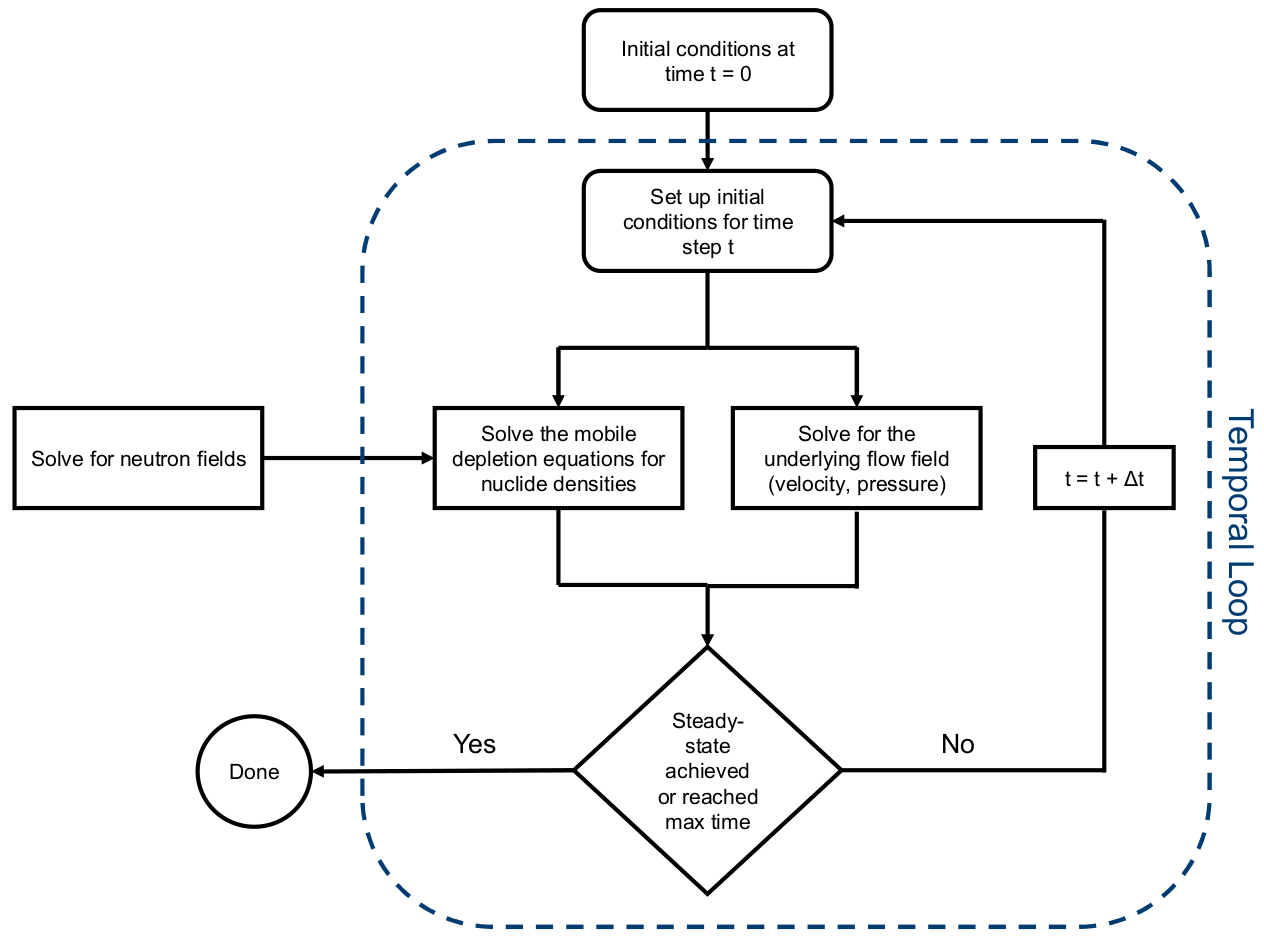
\includegraphics[width=0.95\textwidth]{images/solver/one_way.png}
    \caption{One-way solver coupling between neutron transport and mobile depletion.}
    \label{fig:solver:1_way}
\end{figure}

When considering photon transport for radiological consequence assessment and external dosimery, one must consider the rapid variation of the photon sources caused by the mobile depletion solver. This necessitates the inclusion of the photon transport solve within the inner temporal loop in Figure~\ref{fig:solver:1_way}, resulting in the following modified coupling scheme (Figure~\ref{fig:solver:1_way_photon_neutron}). The flexibility of the multi-app system within \acrshort{moose} allows for the exploration of several other coupling schemes, such as the use of sub-stepping for time integrating different physics over different time scales. This may prove to be useful with coupled photon transport and mobile depletion, as the mobile depletion equations can be sub-stepped with a shorter $\Delta t$ while the photon transport solve can utilize a longer timestep without encountering convergence issues.

\begin{figure}[H]
    \centering
    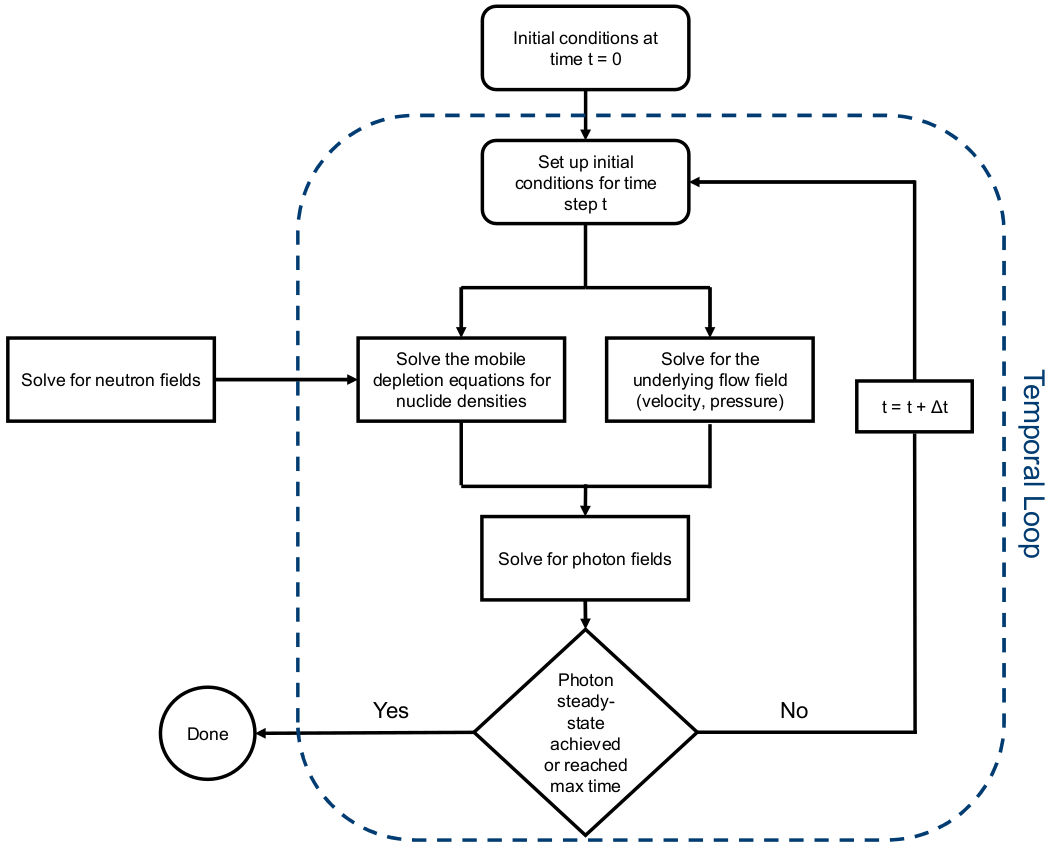
\includegraphics[width=0.95\textwidth]{images/solver/one_way_with_photon.png}
    \caption{Combined photon, neutron, and mobile depletion solver coupling strategy.}
    \label{fig:solver:1_way_photon_neutron}
\end{figure}


\chapter{Verification}
\label{verification}

With the computational approach implemented in \acrshort{moose}, an effort must be made to verify the solvers. This step is crucial to ensure the implementation is correct and to test the numerical accuracy of the methods used for both the radiation transport and mobile depletion packages. To this end, both solvers are independently verified using simple analytical solutions, benchmark problems, and the method of manufactured solutions. This chapter begins by describing the verification strategy and results for the \acrshort{sn} radiation transport solver. Following the verification of the \acrshort{sn} solver, the methods used to mitigate ray effects are verified. Finally, the verification scheme employed for the mobile depletion solver is discussed.

\section{Discrete Ordinates Radiation Transport}
\label{verification:radiation_transport_sn}

The verification of the \acrshort{sn} radiation transport implementation was performed using a simple transport problem to test the space-angle convergence of these methods. This was followed by the use of a series of standard transport benchmark problems, the Kobayashi problems \cite{kobayashi_benchmarks}. While these verification cases are useful to prove the correctness of mono-energetic radiation transport problems, they do not consider the energy dependence of the transport equation. To assess the performance of the transport solver in the multi-group case, a new benchmark problem is proposed using the planned Ontario Tech subcritical assembly.

\subsection{1D Analytical Transport Problem}
\label{verification:radiation_transport_sn:1D_anal}

Consider a 1D infinite slab absorber with a planar particle source placed at $x = 5$ cm emitting isotropically in all directions. The radiation transport equation for this case can be written as the following:
\begin{equation}\label{eq:slab_transport}
    \mu\frac{d}{dx}\psi(x, \mu) + \Sigma_{t}\psi(x,\mu) = \frac{q}{2}\delta(x - 5),\,\,\,\,x\in[-\infty, \infty],\mu\in[-1, 1]\text{.}
\end{equation}
The solution to Eq.~\ref{eq:slab_transport} takes the following form \cite{computational_methods}:
\begin{equation}\label{eq:slab_transport_solution}
    \Phi_{a}(x) = \int_{-1}^{1} \psi(x,\mu)\,d\mu = \frac{q}{2}E_{1}(\Sigma_{t}|x - 5|)\text{,}
\end{equation}
where $E_{1}$ is the exponential integral function of the first kind:
\begin{equation}\label{eq:exp_integral}
    E_{1}(\Sigma_{t}|x - 5|) = \int_{1}^{\infty}\frac{e^{-\Sigma_{t}|x - 5| \gamma}}{\gamma}\,d\gamma\text{;}
\end{equation}
this problem is modelled in \acrshort{gnat} as the first verification problem. This particular problem was chosen for the injection of a strong heterogeneity through the slab radiation source. This work sets the source to $q = 1.0$ s\textsuperscript{-1} and $\Sigma_{t}$ is set to $0.1$ cm\textsuperscript{-1}. An important consideration for this benchmark problem is that the analytical solution is singular as one approaches the slab source:
\begin{equation}
    \lim_{x\rightarrow 5}\frac{q}{2}E_{1}(\Sigma_{t}|x - 5|) = \infty\text{.}
\end{equation}

The numerical solution to this problem applies vacuum boundary conditions at $x = 0$ cm and $x = 10$ cm to emulate the effect of the infinite slab. The domain is meshed with either 10, 100, or 1000 elements with linear Lagrange basis functions. A Legendre quadrature rule is used with either 10, 20, or 40 directions per octant of the unit sphere, resulting in 20, 40, or 80 total directions in 1D as there are two octants of the unit sphere in infinite slab geometry. The \acrfull{pjfnk} solver was used with block Jacobi preconditioning. The largest initial residual vector magnitude across all refinement cases reported by \acrshort{petsc} is $9.974811$, and so a relative convergence convergence criteria of $10^{-8}$ was used. This was found to be sufficient for localizing sources of error to the spatial and angular discretization scheme as further decreases in the relative convergence criteria did not result in substantial changes to the numerical solution. The numerical fluxes, analytical fluxes, and the absolute relative error between the numerical and analytical fluxes can be found in Figures~\ref{fig:verification:1D_flux_10_elem} to \ref{fig:verification:1D_flux_1000_elem}. Both are plotted over the range from $x = 5$ cm to $x = 10$ cm.

\begin{figure}[H]
    \centering
    %\hfill
    \begin{subfigure}[b]{0.495\textwidth}
        \centering
        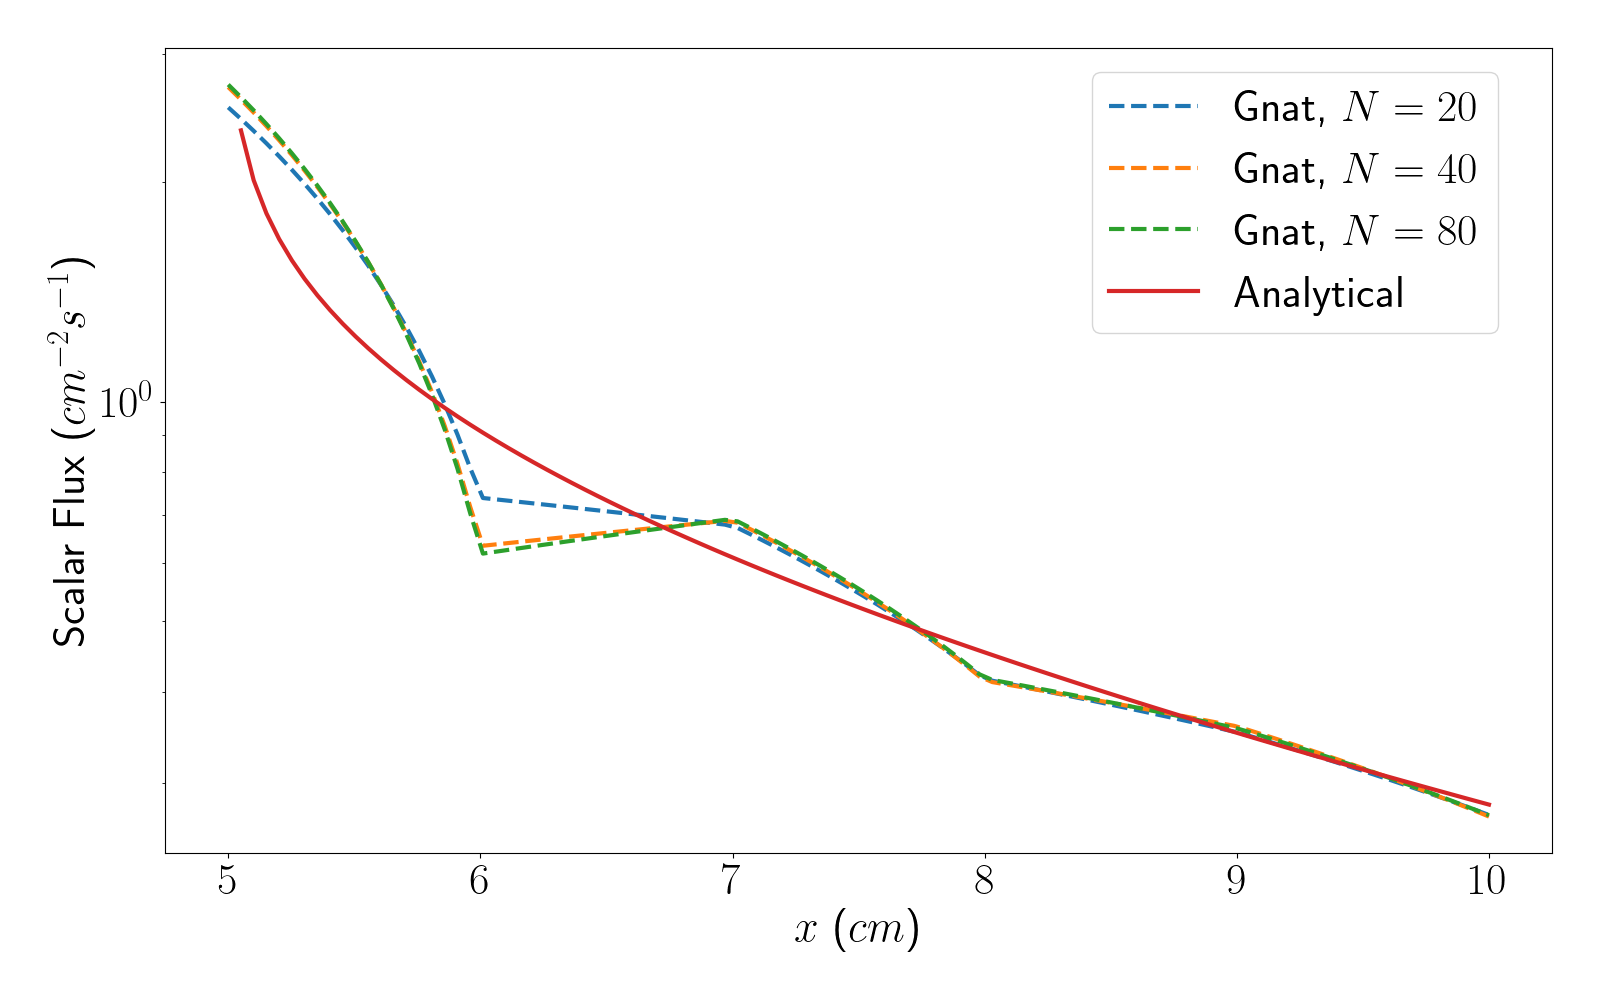
\includegraphics[width=\textwidth]{images/verification/1d_slab/1D_analytical_flux_1.png}
        \caption{Numerical and analytical scalar fluxes.}
        \label{fig:verification:1D_flux:10_elem}
    \end{subfigure}
    \hfill
    \begin{subfigure}[b]{0.495\textwidth}
        \centering
        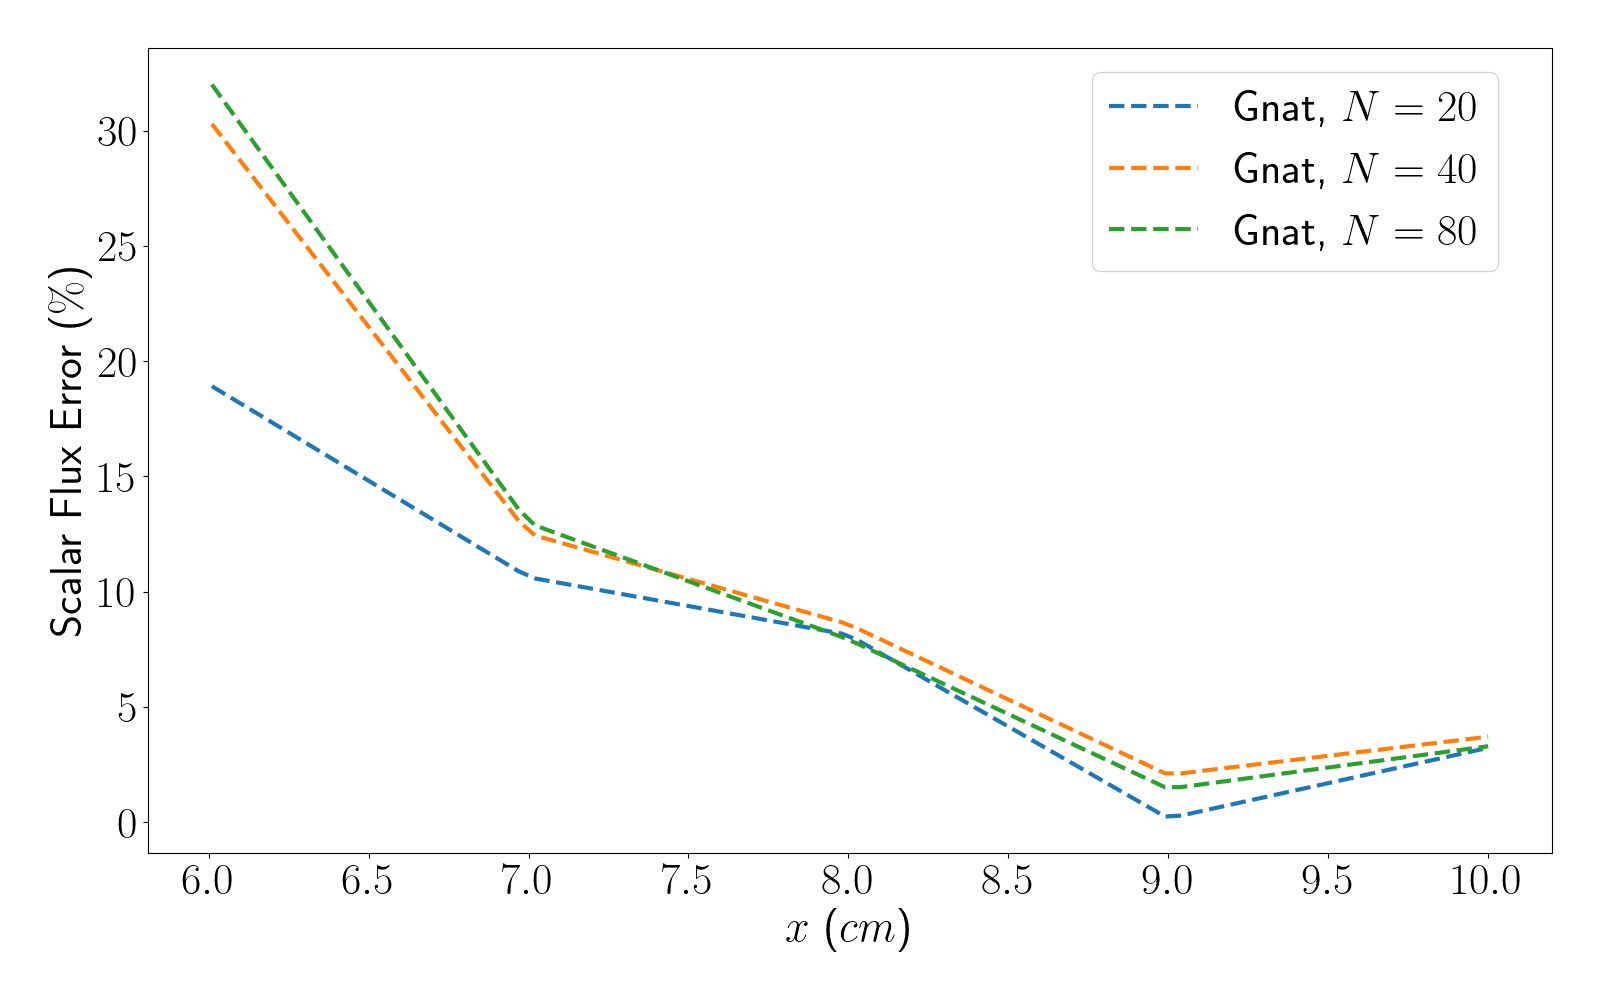
\includegraphics[width=\textwidth]{images/verification/1d_slab/1D_analytical_flux_error_1.png}
        \caption{Relative error in the numerical scalar flux.}
        \label{fig:verification:1D_flux:10_elem_error}
    \end{subfigure}
    \caption{Comparison of the numerical and analytical scalar fluxes for a 10 element mesh.}
    \label{fig:verification:1D_flux_10_elem}
\end{figure}
\begin{figure}[H]
    \centering
    %\hfill
    \begin{subfigure}[b]{0.495\textwidth}
        \centering
        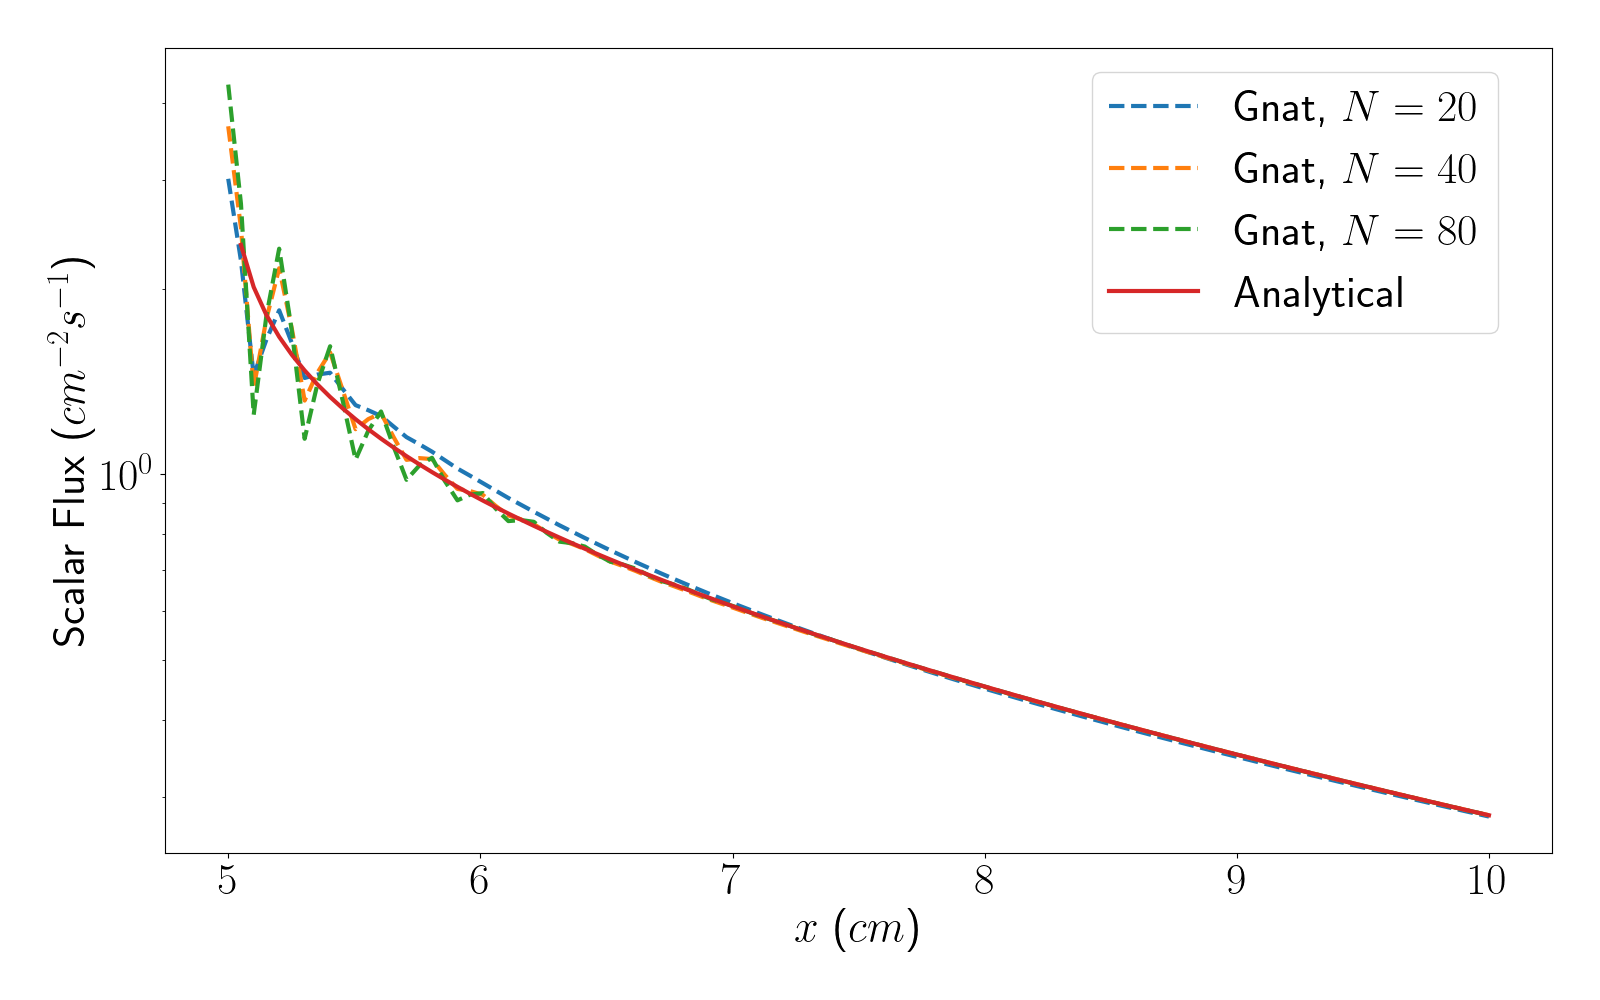
\includegraphics[width=\textwidth]{images/verification/1d_slab/1D_analytical_flux_2.png}
        \caption{Numerical and analytical scalar fluxes.}
        \label{fig:verification:1D_flux:100_elem}
    \end{subfigure}
    \hfill
    \begin{subfigure}[b]{0.495\textwidth}
        \centering
        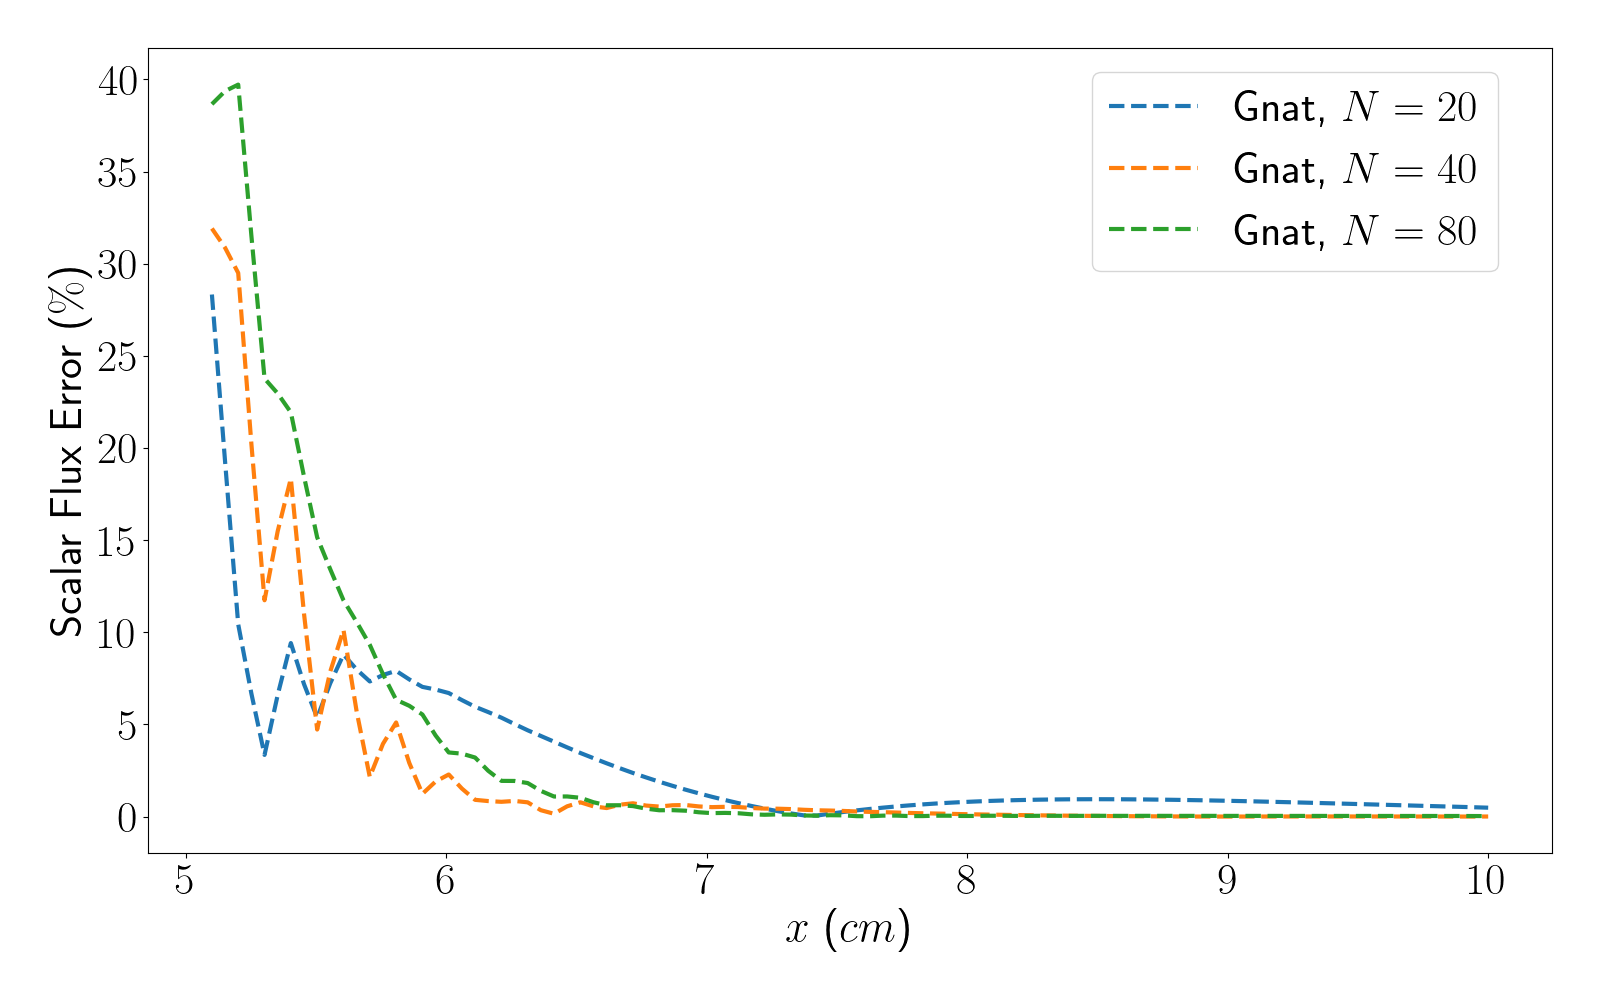
\includegraphics[width=\textwidth]{images/verification/1d_slab/1D_analytical_flux_error_2.png}
        \caption{Relative error in the numerical scalar flux.}
        \label{fig:verification:1D_flux:100_elem_error}
    \end{subfigure}
    \caption{Comparison of the numerical and analytical scalar fluxes for a 100 element mesh.}
    \label{fig:verification:1D_flux_100_elem}
\end{figure}
\begin{figure}[H]
    \centering
    %\hfill
    \begin{subfigure}[b]{0.495\textwidth}
        \centering
        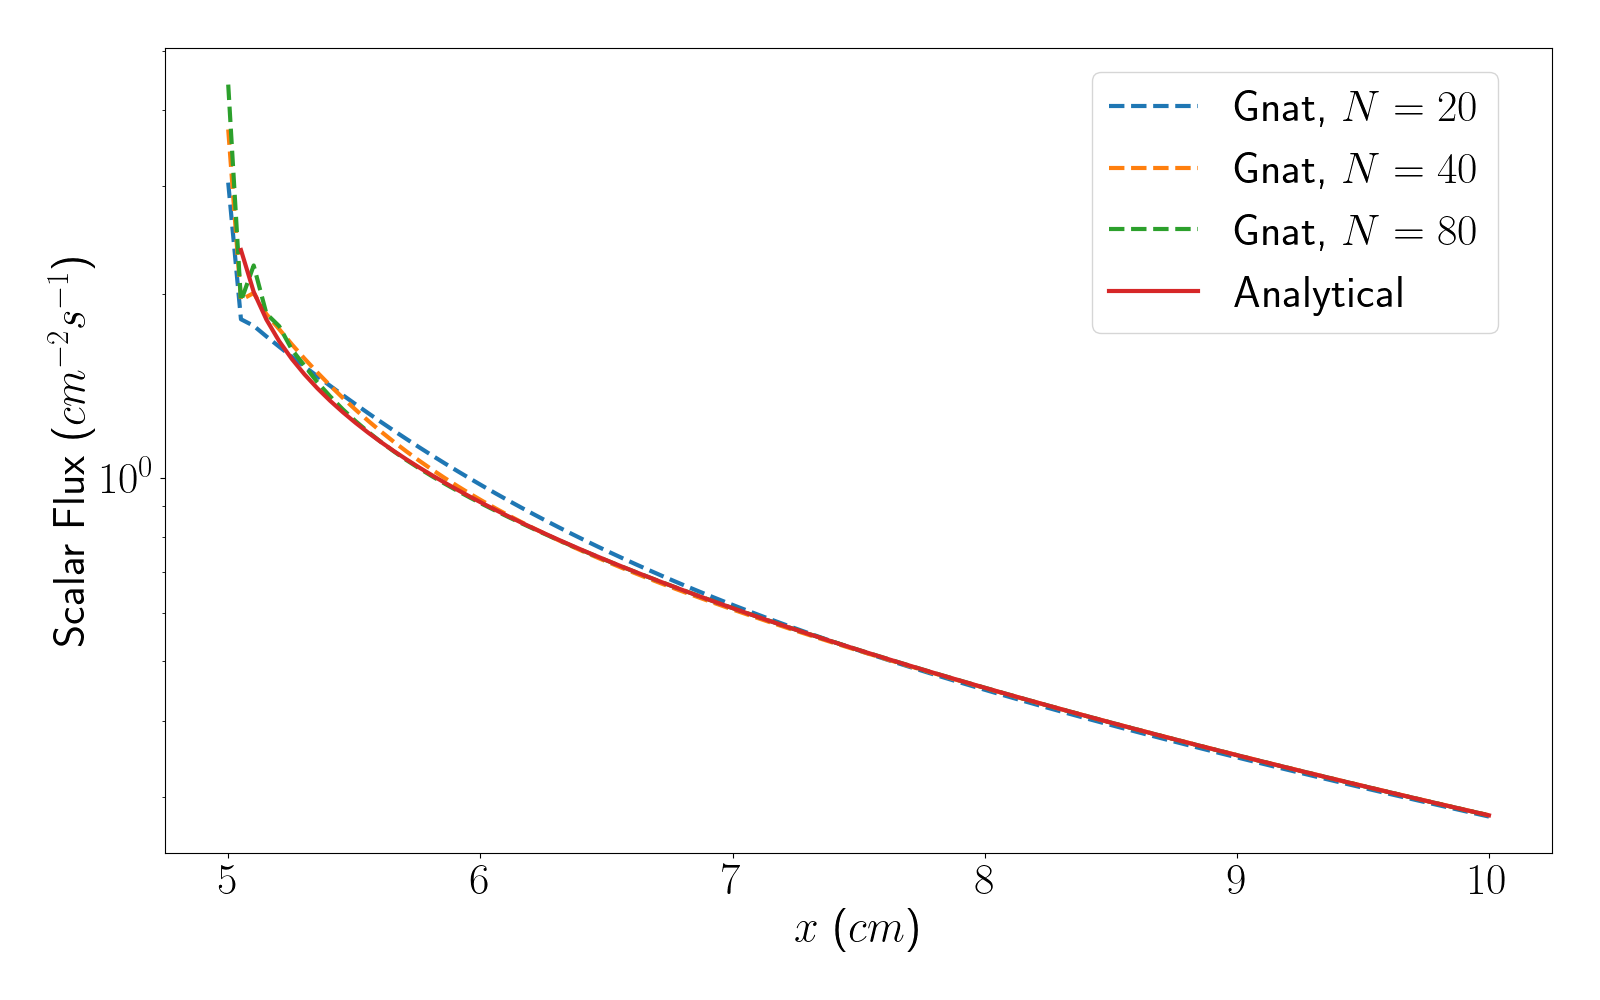
\includegraphics[width=\textwidth]{images/verification/1d_slab/1D_analytical_flux_3.png}
        \caption{Numerical and analytical scalar fluxes.}
        \label{fig:verification:1D_flux:1000_elem}
    \end{subfigure}
    \hfill
    \begin{subfigure}[b]{0.495\textwidth}
        \centering
        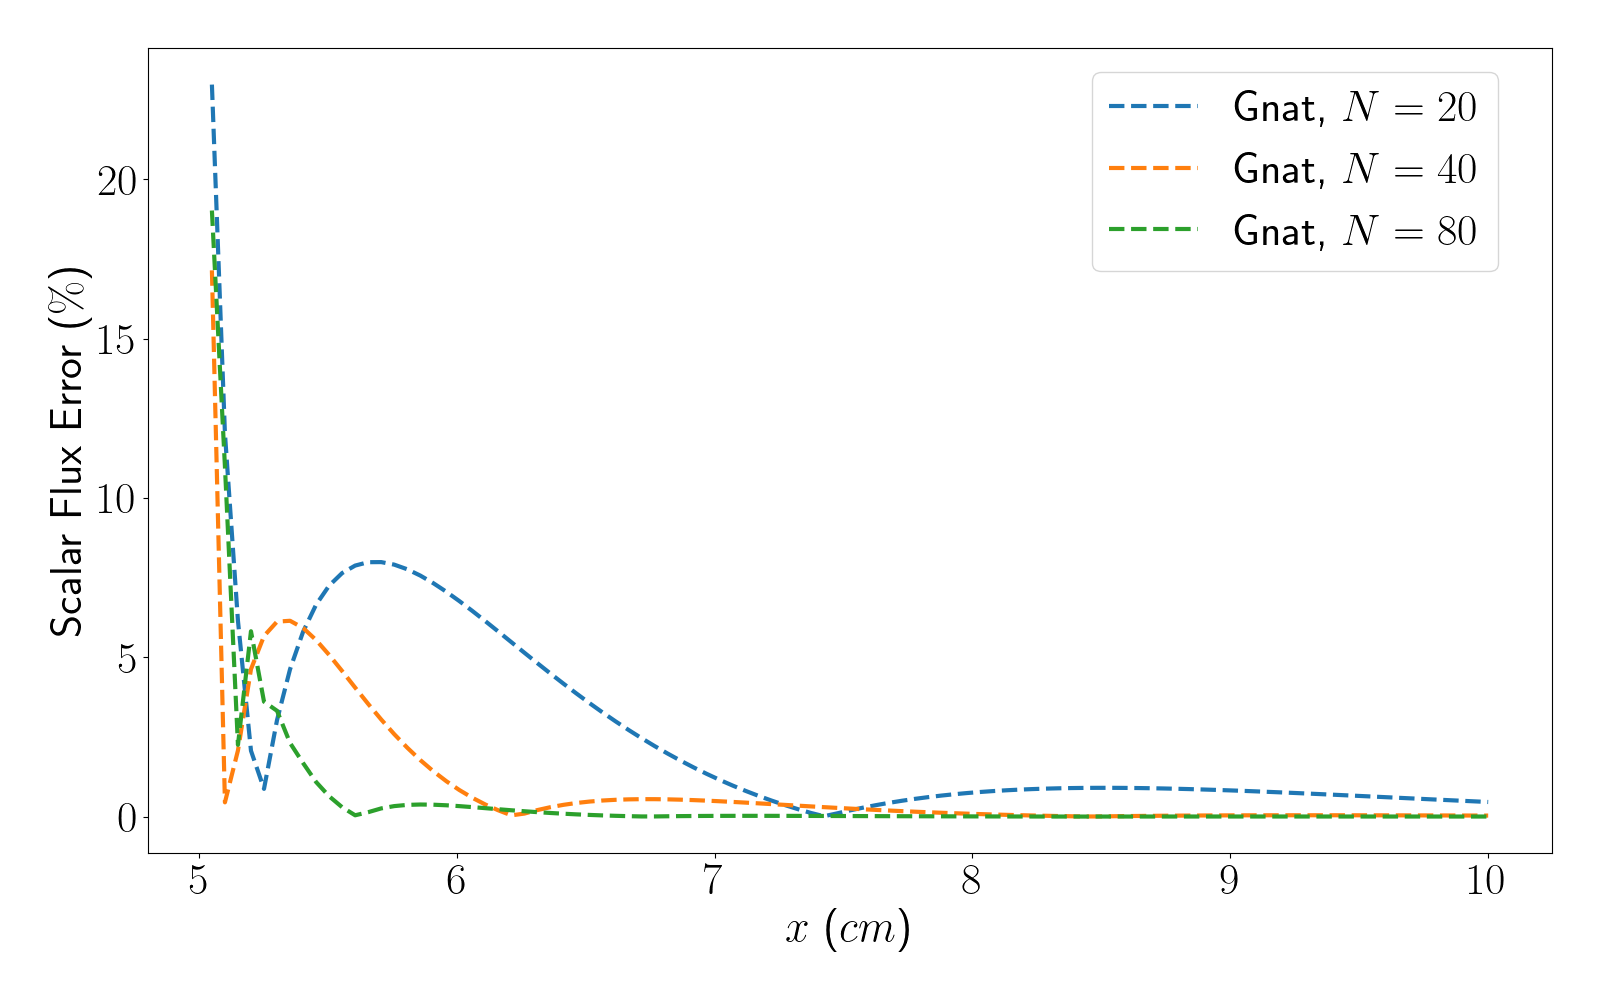
\includegraphics[width=\textwidth]{images/verification/1d_slab/1D_analytical_flux_error_3.png}
        \caption{Relative error in the numerical scalar flux.}
        \label{fig:verification:1D_flux:1000_elem_error}
    \end{subfigure}
    \caption{Comparison of the numerical and analytical scalar fluxes for a 1000 element mesh.}
    \label{fig:verification:1D_flux_1000_elem}
\end{figure}

In the extremely coarse mesh case where only 10 elements are used (Figure~\ref{fig:verification:1D_flux_10_elem}); the numerical scalar fluxes oscillate about the analytical solution by a wide margin with absolute relative errors of up to 30\%. The numerical solution entirely fails to represent the analytical scalar flux at $x = 5$ cm. Refinement in the angular domain does not result in an increase in accuracy for these coarse mesh results; the additional angular directions only serve to further increase the scalar flux error near the source. However, the scalar flux error decreases as the fluxes move further away from the slab source indicating that this localized heterogeneity is responsible for the instability of the numerical fluxes. Moving to 100 elements (Figure~\ref{fig:verification:1D_flux_100_elem}), the numerical solutions begin to capture the analytical solution closer to the slab source and additional angular refinement results in improvements in the prediction of the analytical solution further downwind from $x = 5$ cm. The peak error rises to 40\% near the source, which is likely caused by the singularity previously discussed. At the final refinement of 1000 elements, the angular resolution of the problem starts to dominate the error in the numerical solution. The low order quadrature set with 10 directions per octant overshoots the analytical solution. Refining the angular quadrature to 40 directions per octant results in a decrease in the relative error to near-zero everywhere with the exception of the neighborhood near the slab source. The convergence to the analytical solution as the angular domain is refined lends credibility to the implementation of the \acrshort{sn} transport solver.

\subsection{The Kobayashi Benchmarks}
\label{verification:radiation_transport_sn:kobayashi}

The next series of verification problems are the Kobayashi benchmark problems \cite{kobayashi_benchmarks}. These have become a series of standard transport benchmarks due to the presence of a large void regions and several order of magnitude jump discontinuities in cross section, which are challenging for second order transport methods (such as the \acrshort{saaf} method) to resolve. These large void regions are also set up such that they result in long streaming paths and deep penetrations, which are challenging for the \acrshort{sn} method to accurately predict due to ray effects. There are six benchmark problems in the Kobayashi suite: three problems that use pure absorbers and three problems that use a scattering ratio of $\Sigma_{s} / \Sigma_{t} = 0.5$. This work elects to verify the \acrshort{sn} radiation transport solver with the scattering cases to test as many capabilities of the solver in 3D as possible. All of the benchmark problems use the material properties in Table~\ref{table:kobayashi_props} \cite{kobayashi_benchmarks}. The volumetric particle source and the scattering cross sections are isotropic.
\begin{table}[H]
    \centering
    \singlespacing
    \caption[Material properties for the Kobayashi benchmark problems.]{Material properties for the Kobayashi benchmark problems. Adapted from Kobayashi and Sugimura \cite{kobayashi_benchmarks}.}
    \begin{tabular}{|cccc|}
        \hline
        \textbf{Region} & \makecell{$Q^{\text{ext}}$ \\ cm\textsuperscript{-3} s\textsuperscript{-1}} & \makecell{$\Sigma_{t}$ \\ cm\textsuperscript{-1}}  & \makecell{$\Sigma_{s}$ \\ cm\textsuperscript{-1}} \\
        \hline
        1 & $1.0$ & $1\times10^{-1}$ & $5\times 10^{-2}$\\
        2 & $0.0$ & $1\times10^{-4}$ & $5\times 10^{-5}$\\
        3 & $0.0$ & $1\times10^{-1}$ & $5\times 10^{-2}$\\
        \hline
    \end{tabular}
    \label{table:kobayashi_props}
\end{table}

The first of these benchmark problems is a square particle source embedded in a voided regions, which is then surrounded by a shield. Reflective boundary conditions are applied along the x-z plane ($y = 0\text{ cm}$), x-y plane ($z = 0\text{ cm}$) and y-z plane ($x = 0\text{ cm}$). Vacuum boundary conditions are applied along the x-z plane ($y = 100\text{ cm}$), x-y plane ($z = 100\text{ cm}$) and y-z plane ($x = 100\text{ cm}$). The geometry of the first benchmark problem can be found in Figure~\ref{fig:verification:sn_kobayashi_1_geo}. The second benchmark problem is a square particle source embedded in a shield. There is a straight voided duct penetrating this shield, starting from the particle source and moving through the domain until it reaches a vacuum boundary. Reflective boundary conditions are applied along the x-z plane ($y = 0\text{ cm}$), x-y plane ($z = 0\text{ cm}$) and y-z plane ($x = 0\text{ cm}$). Vacuum boundary conditions are applied along the x-z plane ($y = 100\text{ cm}$), x-y plane ($z = 60\text{ cm}$) and y-z plane ($x = 60\text{ cm}$). The geometry of this benchmark problem can be found in Figure~\ref{fig:verification:sn_kobayashi_2_geo}.
\begin{figure}[H]
    \centering
    \begin{subfigure}[b]{0.45\textwidth}
        \centering
        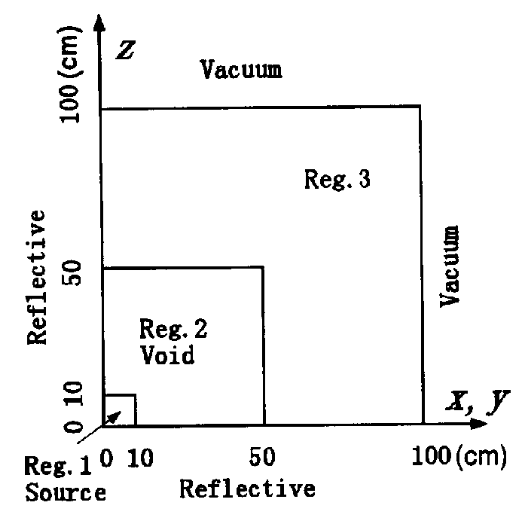
\includegraphics[width=\textwidth]{images/verification/sn_kobayashi/geometry/1_geo_1.png}
        \caption{x-y / y-z plane for the first Kobayashi problem.}
        \label{fig:verification:sn_kobayashi_1_geo:1}
    \end{subfigure}
    \hfill
    \begin{subfigure}[b]{0.45\textwidth}
        \centering
        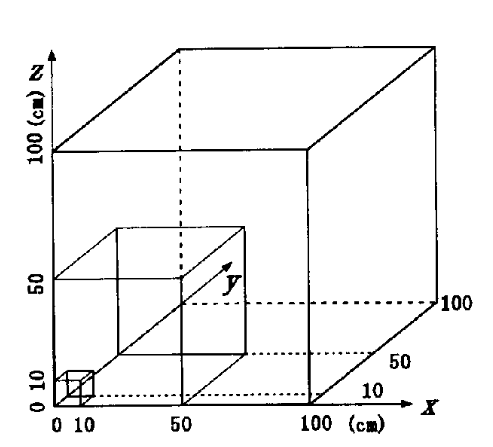
\includegraphics[width=\textwidth]{images/verification/sn_kobayashi/geometry/1_geo_2.png}
        \caption{Sketch of the first problem.}
        \label{fig:verification:sn_kobayashi_1_geo:2}
    \end{subfigure}
    \caption[Geometry for the first Kobayashi problem.]{Geometry for the first Kobayashi problem. Taken from Kobayashi and Sugimura \cite{kobayashi_benchmarks}.}
    \label{fig:verification:sn_kobayashi_1_geo}
\end{figure}
\begin{figure}[H]
    \centering
    \begin{subfigure}[b]{0.45\textwidth}
        \centering
        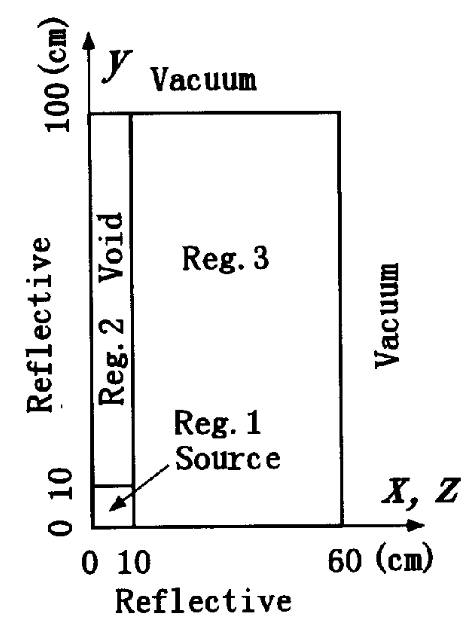
\includegraphics[width=\textwidth]{images/verification/sn_kobayashi/geometry/2_geo_1.png}
        \caption{x-y / y-z plane for the second Kobayashi problem.}
        \label{fig:verification:sn_kobayashi_2_geo:1}
    \end{subfigure}
    \hfill
    \begin{subfigure}[b]{0.45\textwidth}
        \centering
        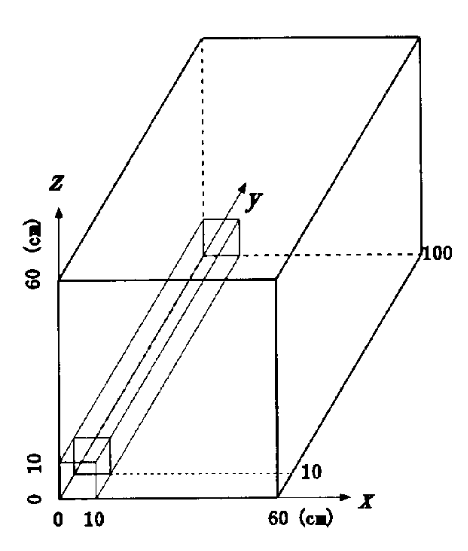
\includegraphics[width=\textwidth]{images/verification/sn_kobayashi/geometry/2_geo_2.png}
        \caption{Sketch of the second problem.}
        \label{fig:verification:sn_kobayashi_2_geo:2}
    \end{subfigure}
    \caption[Geometry for the second Kobayashi problem.]{Geometry for the second Kobayashi problem. Taken from Kobayashi and Sugimura \cite{kobayashi_benchmarks}.}
    \label{fig:verification:sn_kobayashi_2_geo}
\end{figure}
The third benchmark problem is a square particle source embedded in a shield. There is a voided duct penetrating the shielded region, starting at the particle source, taking three right angle turns, and exiting the domain at a vacuum boundary. Similar to the previous benchmark problems, reflective boundary conditions are applied along the x-z plane ($y = 0\text{ cm}$), x-y plane ($z = 0\text{ cm}$) and y-z plane ($x = 0\text{ cm}$). Vacuum boundary conditions are applied along the x-z plane ($y = 100\text{ cm}$), x-y plane ($z = 60\text{ cm}$) and y-z plane ($x = 60\text{ cm}$). The benchmark geometry for this dog-legged duct can be found in Figure~\ref{fig:verification:sn_kobayashi_3_geo}.
\begin{figure}[H]
    \centering
    \begin{subfigure}[b]{0.45\textwidth}
        \centering
        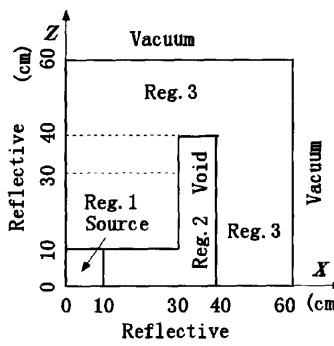
\includegraphics[width=\textwidth]{images/verification/sn_kobayashi/geometry/3_geo_1.png}
        \caption{x-z plane for the third Kobayashi problem.}
        \label{fig:verification:sn_kobayashi_3_geo:1}
    \end{subfigure}
    \hfill
    \begin{subfigure}[b]{0.45\textwidth}
        \centering
        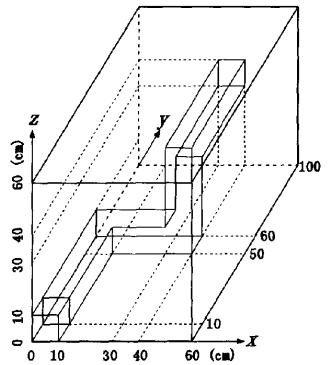
\includegraphics[width=\textwidth]{images/verification/sn_kobayashi/geometry/3_geo_2.png}
        \caption{Sketch of the third problem.}
        \label{fig:verification:sn_kobayashi_3_geo:2}
    \end{subfigure}
    \caption[Geometry for the third Kobayashi problem.]{Geometry for the third Kobayashi problem. Taken from Kobayashi and Sugimura \cite{kobayashi_benchmarks}.}
    \label{fig:verification:sn_kobayashi_3_geo}
\end{figure}

Numerical solutions to these three benchmark problems were conducted before the reflective boundary condition implementation in \acrshort{gnat} was complete. The mesh for the problem was unfolded across the x-z ($y = 0\text{ cm}$), x-y ($z = 0\text{ cm}$) and y-z ($x = 0\text{ cm}$) planes. This increases the size of the problem and places the source at the center of the domain to compensate for this deficiency. Each benchmark problem was meshed using uniform quadrilateral elements with side lengths of $5$ cm. This resulted in 72,000 elements in the first benchmark, 25,920 elements in the second problem, and 23,040 elements in the third problem. The finite element basis functions used were linear Lagrange functions. All benchmark cases used the \acrshort{pjfnk} solver with preconditioning provided by the hypre package BoomerAMG and 30 \acrfull{gmres} vectors. All benchmark problems are solved with a Gauss-Chebyshev angular quadrature set. The first benchmark problem used 10 polar angles and 10 azimuthal angles per octant of the unit sphere, resulting in a total of 800 angular directions. The second and third benchmark problems used 16 azimuthal angles and 12 polar angles per octant of the unit sphere for a total of 1536 angular directions. An initial residual vector magnitude of $3.339351\times 10^{3}$ was obtained for the first problem, which was the largest across each of the Kobayashi benchmarks. This led to the use of a relative convergence criteria of $10^{-12}$ to ensure that the magnitude of the final residual vector was below $10^{-8}$ on convergence. Experimentation with a reduced order angular quadrature showed that any additional refinement of the relative convergence criteria did not result in any substantial changes to the result of the Kobayashi problems.

\begin{figure}[H]
    \centering
    \begin{subfigure}[b]{0.4\textwidth}
        \centering
        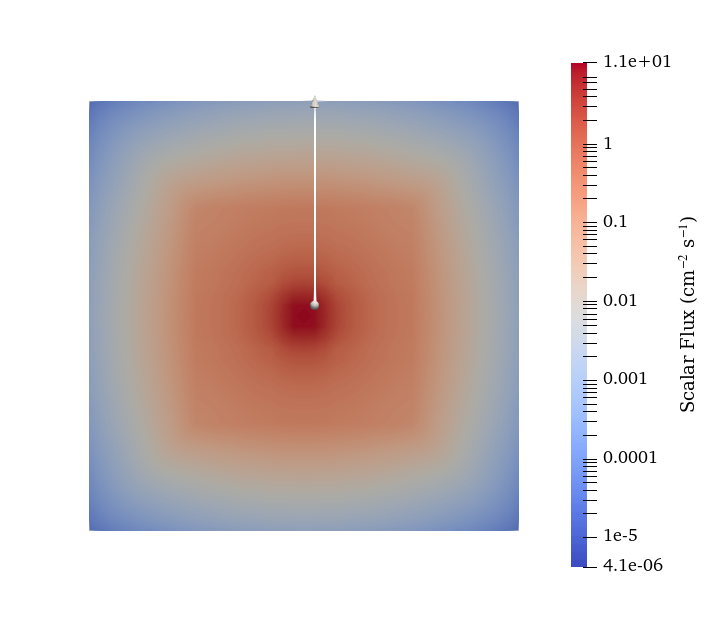
\includegraphics[width=\textwidth]{images/verification/sn_kobayashi/1/kobayashi_1a_flux_map.png}
        \caption{Scalar flux distribution associated with the line plot. The cutting plane is the x-y plane at $z = 5\text{ cm}$.}
        \label{fig:verification:sn_kobayashi_1a:flux}
    \end{subfigure}
    \hfill
    \begin{subfigure}[b]{0.59\textwidth}
        \centering
        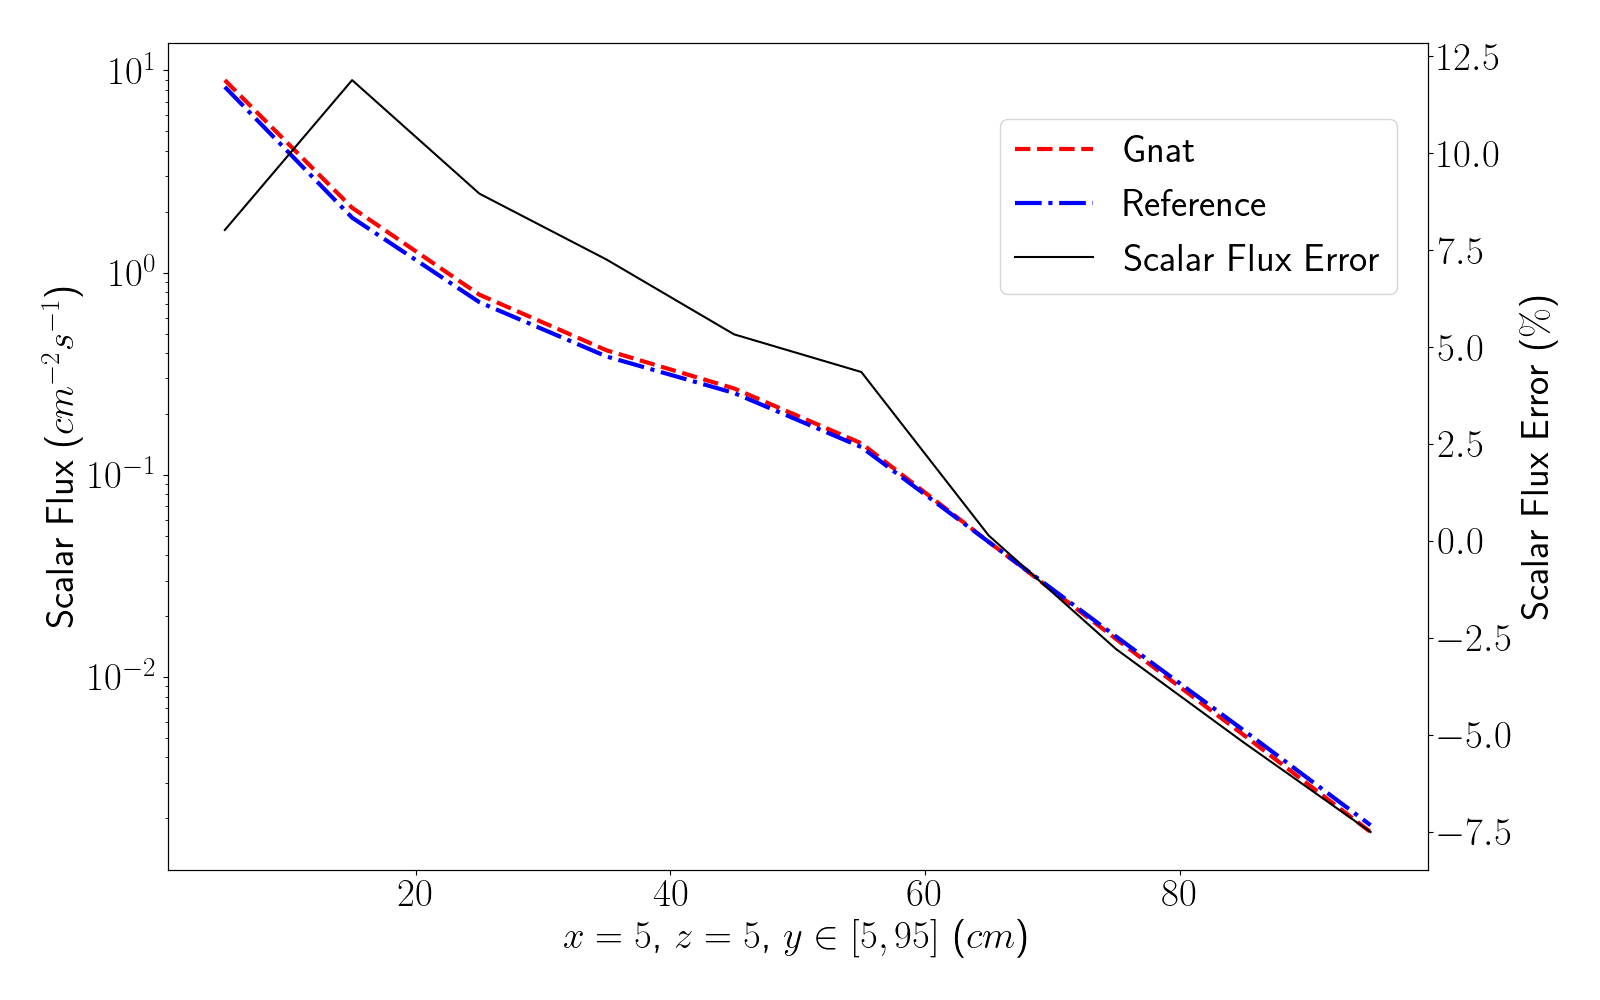
\includegraphics[width=\textwidth]{images/verification/sn_kobayashi/1/kobayashi_1a.png}
        \caption{Comparison with the benchmark problem. Reference taken from Kobayashi and Sugimura \cite{kobayashi_benchmarks}.}
        \label{fig:verification:sn_kobayashi_1a:line_plot}
    \end{subfigure}
    \caption{Results of the Kobayashi benchmark 1a.}
    \label{fig:verification:sn_kobayashi_1a}
\end{figure}

\begin{figure}[H]
    \centering
    \begin{subfigure}[b]{0.4\textwidth}
        \centering
        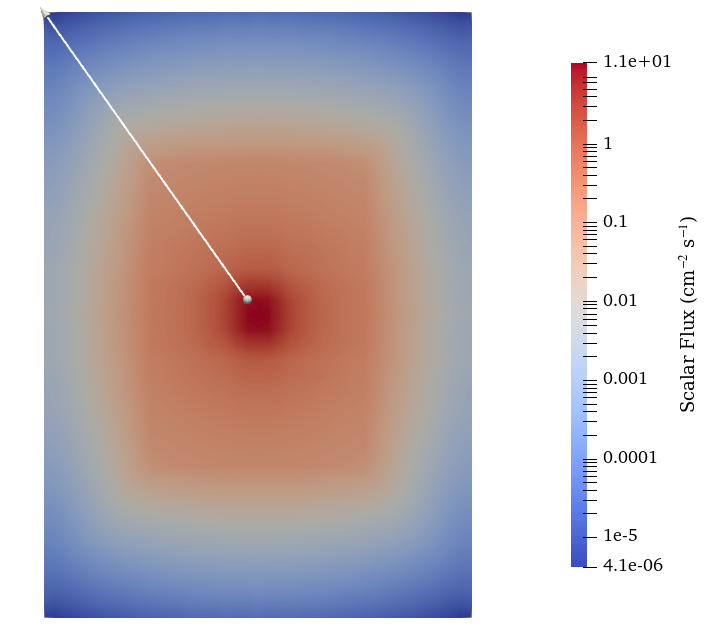
\includegraphics[width=\textwidth]{images/verification/sn_kobayashi/1/kobayashi_1b_flux_map.png}
        \caption{Scalar flux distribution associated with the line plot. The cutting plane has a normal vector of $\{-1/\sqrt{2}, -1/\sqrt{2}, 0\}$ and passes through the point $\{5\text{ cm}, 5\text{ cm}, 5\text{ cm}\}$.}
        \label{fig:verification:sn_kobayashi_1b:flux}
    \end{subfigure}
    \hfill
    \begin{subfigure}[b]{0.59\textwidth}
        \centering
        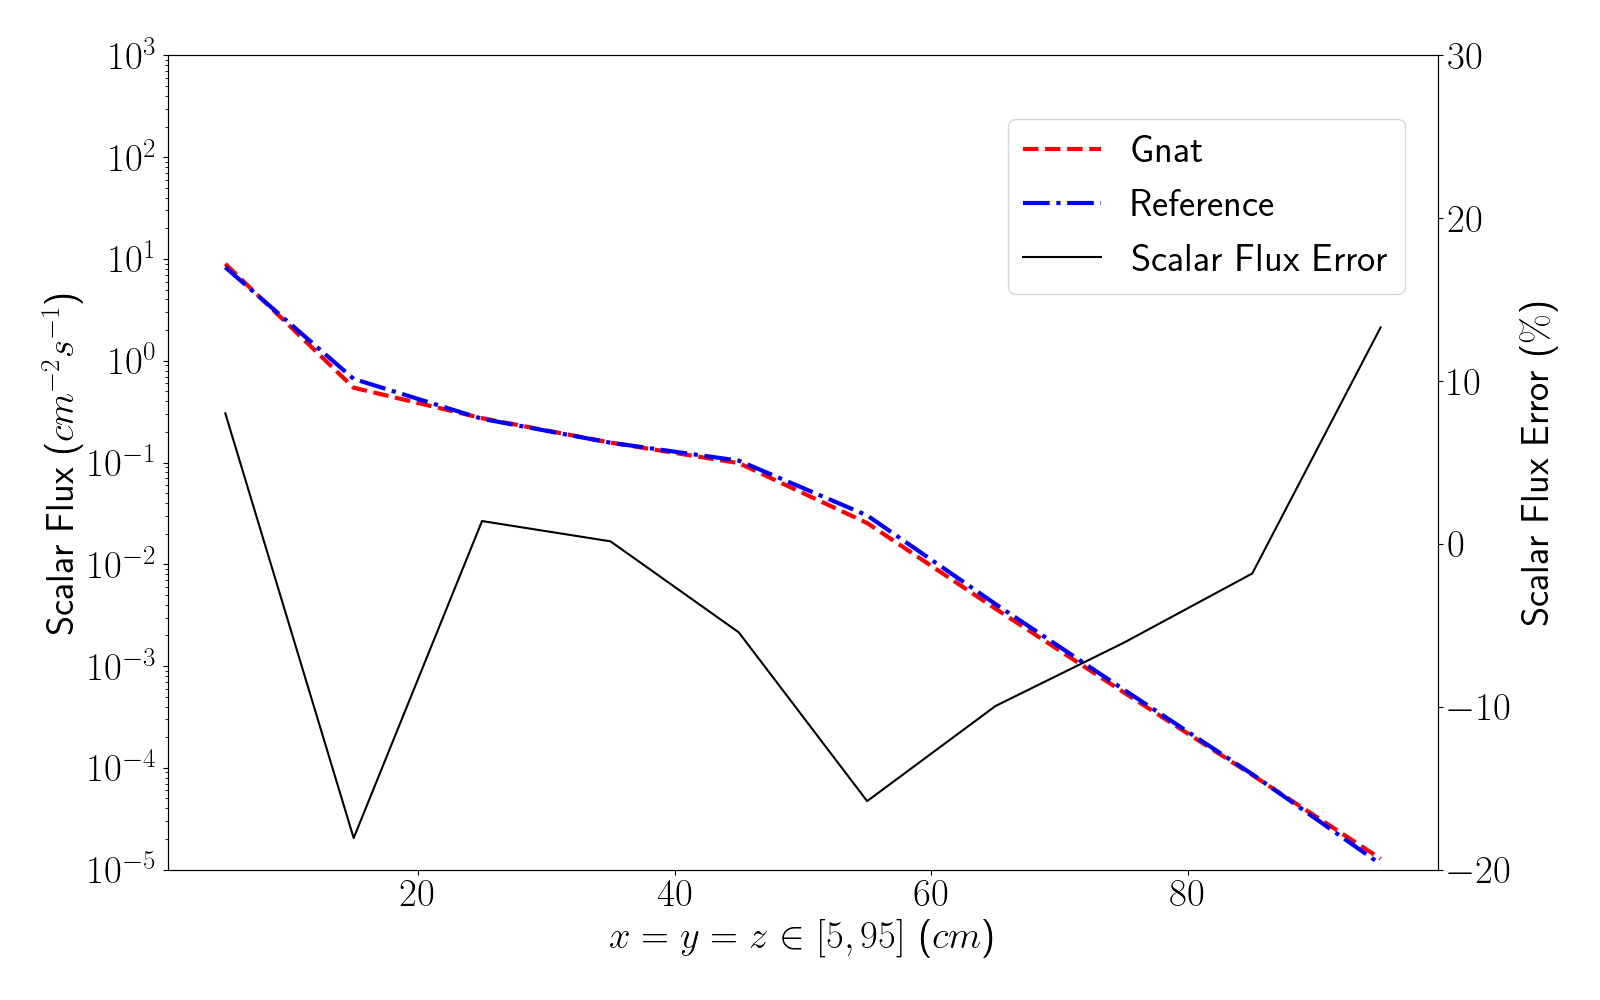
\includegraphics[width=\textwidth]{images/verification/sn_kobayashi/1/kobayashi_1b.png}
        \caption{Comparison with the benchmark problem. Reference taken from Kobayashi and Sugimura \cite{kobayashi_benchmarks}.}
        \label{fig:verification:sn_kobayashi_1b:line_plot}
    \end{subfigure}
    \caption{Results of the Kobayashi benchmark 1b.}
    \label{fig:verification:sn_kobayashi_1b}
\end{figure}

\begin{figure}[H]
    \centering
    \begin{subfigure}[b]{0.4\textwidth}
        \centering
        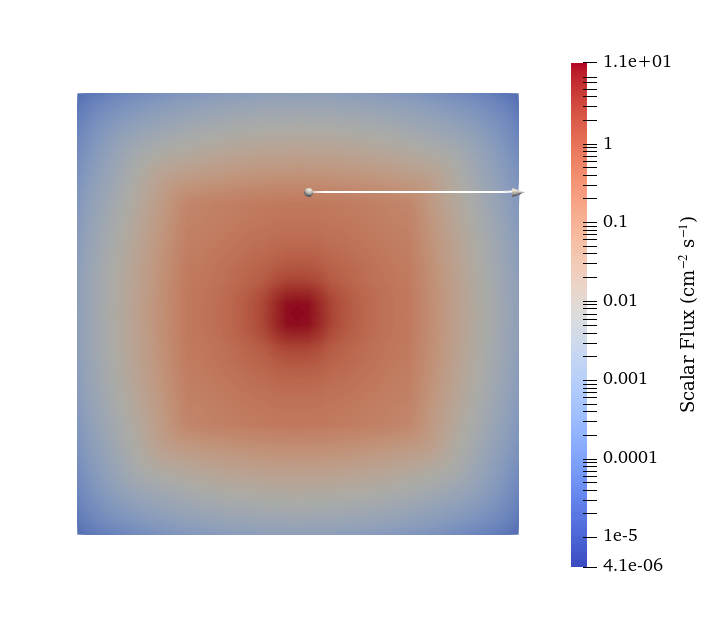
\includegraphics[width=\textwidth]{images/verification/sn_kobayashi/1/kobayashi_1c_flux_map.png}
        \caption{Scalar flux distribution associated with the line plot. The cutting plane is the x-y plane at $z = 5\text{ cm}$.}
        \label{fig:verification:sn_kobayashi_1c:flux}
    \end{subfigure}
    \hfill
    \begin{subfigure}[b]{0.59\textwidth}
        \centering
        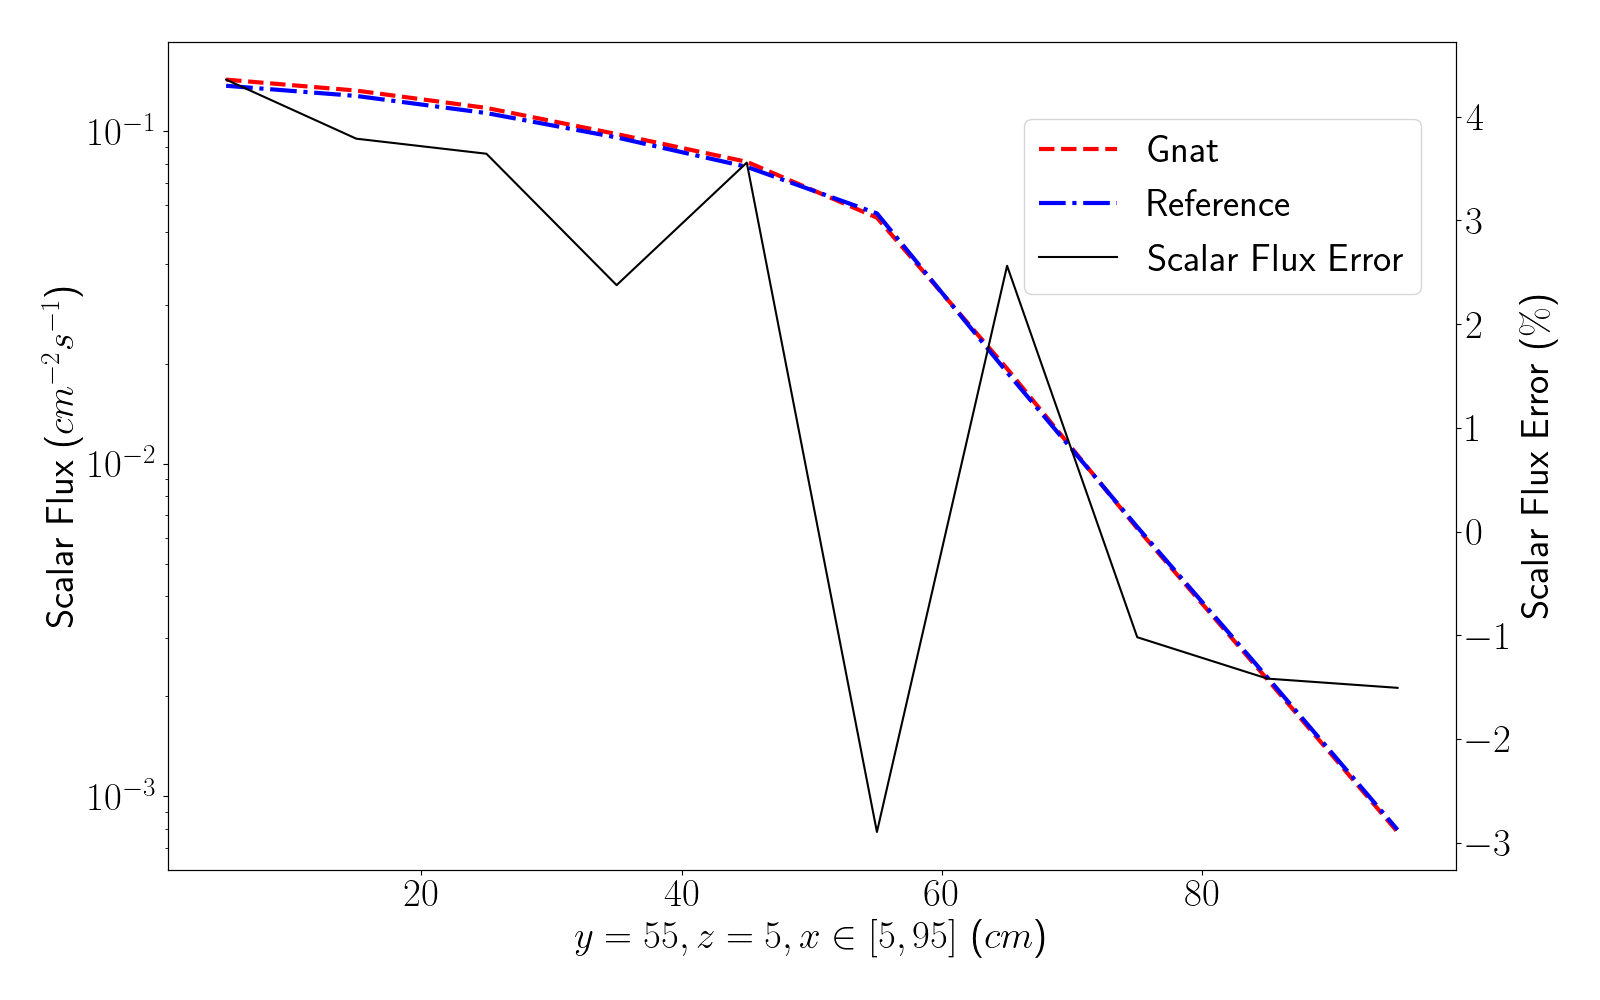
\includegraphics[width=\textwidth]{images/verification/sn_kobayashi/1/kobayashi_1c.png}
        \caption{Comparison with the benchmark problem. Reference taken from Kobayashi and Sugimura \cite{kobayashi_benchmarks}.}
        \label{fig:verification:sn_kobayashi_1c:line_plot}
    \end{subfigure}
    \caption{Results of the Kobayashi benchmark 1c.}
    \label{fig:verification:sn_kobayashi_1c}
\end{figure}

The results for the first benchmark problem can be found in Figures~\ref{fig:verification:sn_kobayashi_1a} to \ref{fig:verification:sn_kobayashi_1c} where they are compared with the solutions obtained by Kobayashi and Sugimura \cite{kobayashi_benchmarks}. In general, the results obtained with the \acrshort{sn} method using the \acrshort{saaf} spatial discretization agree well with the benchmark problem. In the case of Figure~\ref{fig:verification:sn_kobayashi_1a:line_plot} the relative scalar flux error reaches a maximum along the interface between the voided region and the particle source, which represents a large jump discontinuity in both cross section and the particle source. The uniform meshing scheme with the level of coarseness used is unable to capture that discontinuity, resulting in an over-prediction error. In the case of Figure~\ref{fig:verification:sn_kobayashi_1b:line_plot} this behavior is amplified by the point discontinuity at both the corner of the particle source and the interior corner of the shield, resulting in the two error peaks at 15 cm and 55 cm. The numerical scalar flux solution behaves quite well in the case of the lined plotted in Figure~\ref{fig:verification:sn_kobayashi_1c:line_plot} where the maximum error occurs at the corner of the shield. In general, the \acrshort{sn} solver proves to be capable of predicting the behavior of the first Kobayashi problem over the majority of the domain, with particularly good performance in regions that do not have large jump discontinuities in material properties or sources. 

The results for the second benchmark problem can be found in Figure~\ref{fig:verification:sn_kobayashi_2a} and Figure~\ref{fig:verification:sn_kobayashi_2b}. This duct problem is prone to ray effects when solved with \acrshort{sn} transport solvers due to the presence of a long streaming path moving from the localized particle source to the vacuum boundary. It can be seen that the error starts at 10\%, decreases, and then starts increasing over the plotted line in Figure~\ref{fig:verification:sn_kobayashi_2a:line_plot} until it reaches a maximum at 95 cm. This increase in error over the duct is caused by ray effects and the cross section discontinuity along the edge of the duct, which can be further visualized in Figure~\ref{fig:verification:sn_kobayashi_2b:line_plot}. The error in the numerical scalar flux starts at 40\% and drops to -40\% over the length of the duct. The scalar flux plotted through the diffuse region of the domain remains error-free by comparison. This indicates that not enough directions have been provided to properly resolve this deep penetration, especially when compared to the number of directions required to resolve the first benchmark problem.  
\begin{figure}[H]
    \centering
    \begin{subfigure}[b]{0.4\textwidth}
        \centering
        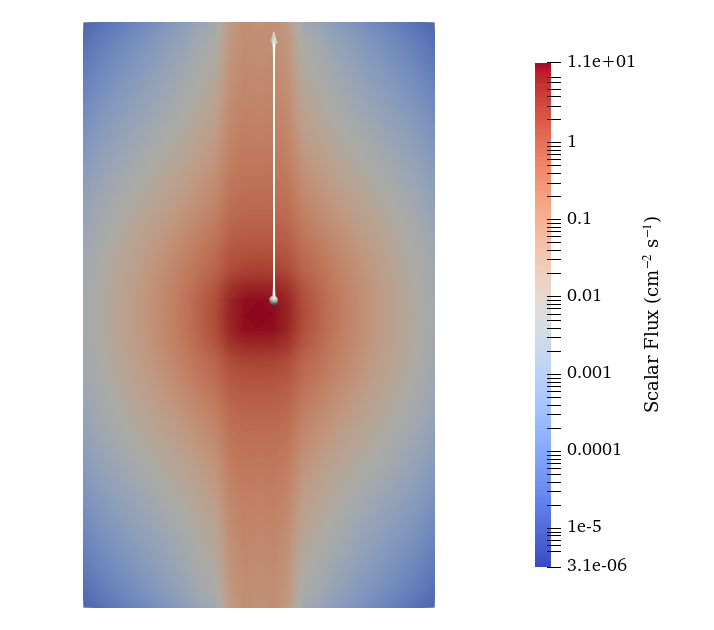
\includegraphics[width=\textwidth]{images/verification/sn_kobayashi/2/kobayashi_2a_flux_map.png}
        \caption{Scalar flux distribution associated with the line plot. The cutting plane is the x-y plane at $z = 5\text{ cm}$.}
        \label{fig:verification:sn_kobayashi_2a:flux}
    \end{subfigure}
    \hfill
    \begin{subfigure}[b]{0.59\textwidth}
        \centering
        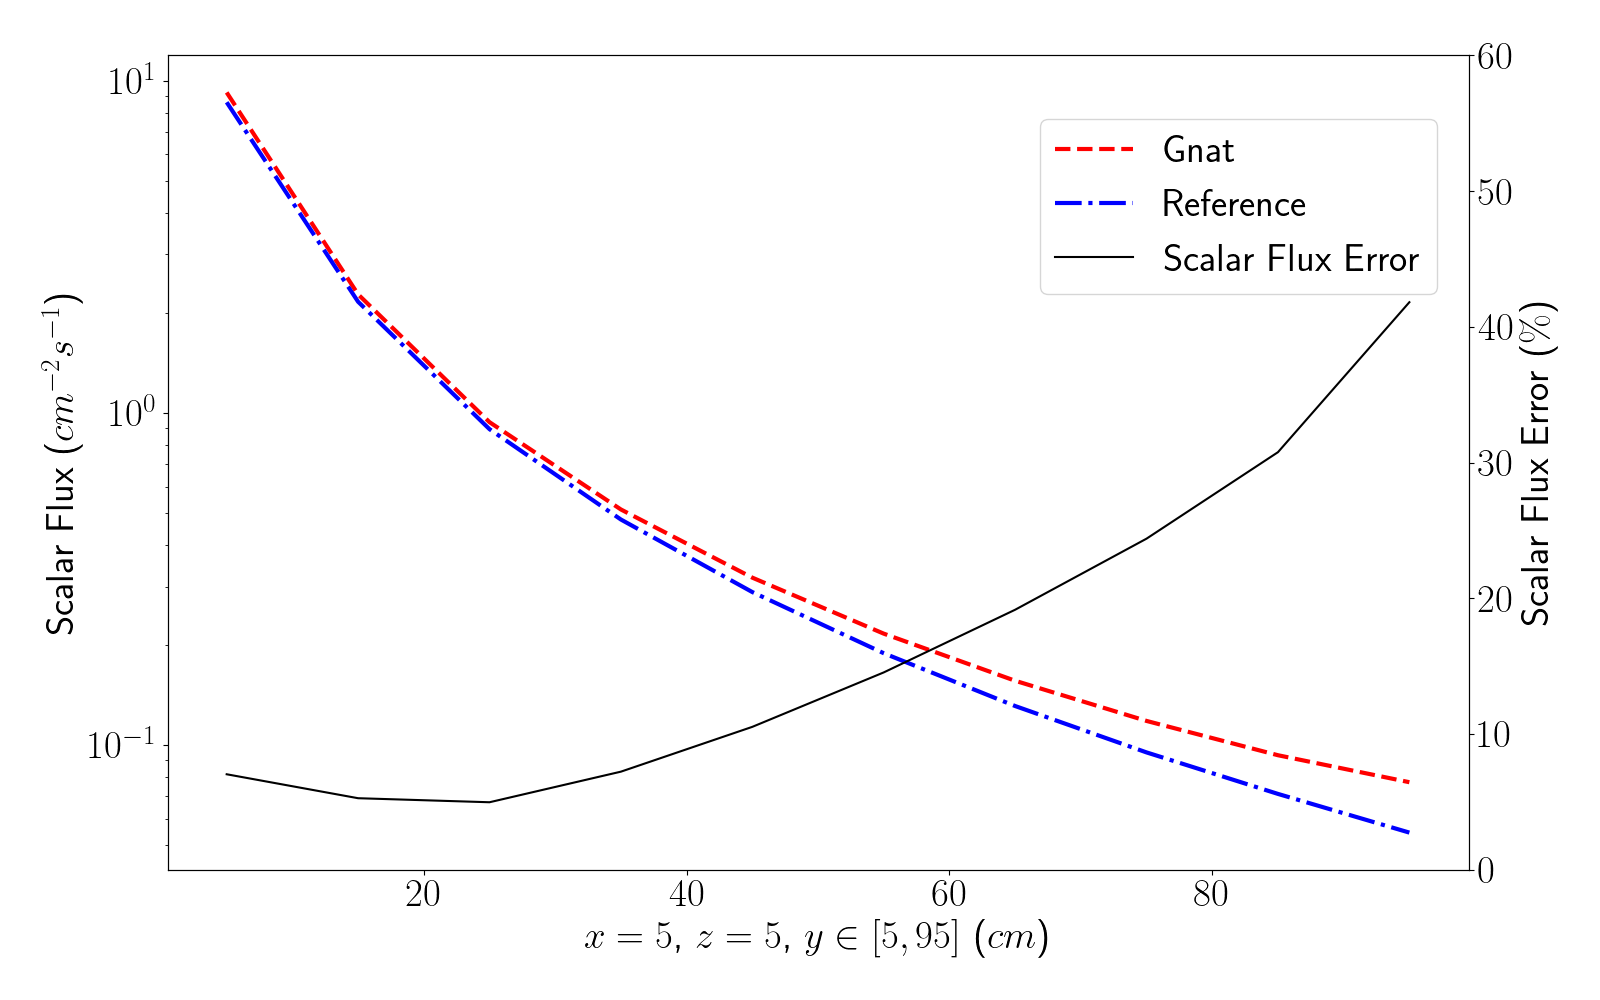
\includegraphics[width=\textwidth]{images/verification/sn_kobayashi/2/kobayashi_2a.png}
        \caption{Comparison with the benchmark problem. Reference taken from Kobayashi and Sugimura \cite{kobayashi_benchmarks}.}
        \label{fig:verification:sn_kobayashi_2a:line_plot}
    \end{subfigure}
    \caption{Results of the Kobayashi benchmark 2a.}
    \label{fig:verification:sn_kobayashi_2a}
\end{figure}

\begin{figure}[H]
    \centering
    \begin{subfigure}[b]{0.4\textwidth}
        \centering
        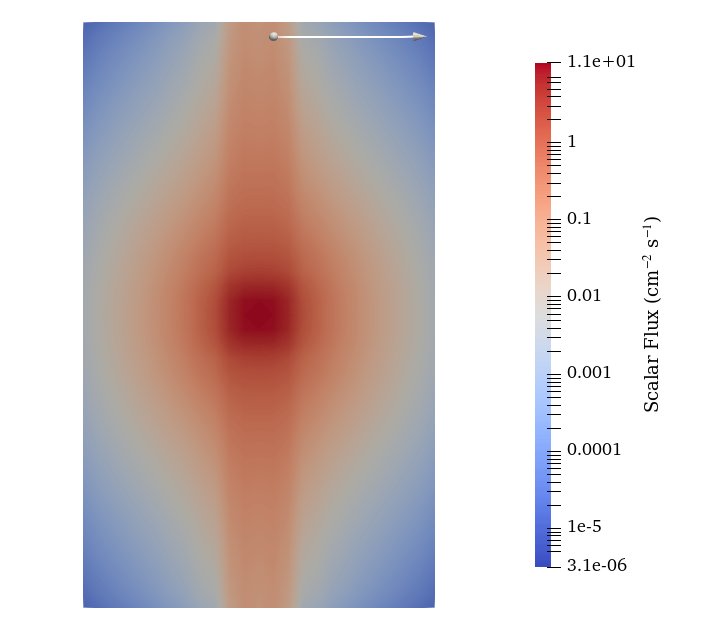
\includegraphics[width=\textwidth]{images/verification/sn_kobayashi/2/kobayashi_2b_flux_map.png}
        \caption{Scalar flux distribution associated with the line plot. The cutting plane is the x-y plane at $z = 5\text{ cm}$.}
        \label{fig:verification:sn_kobayashi_2b:flux}
    \end{subfigure}
    \hfill
    \begin{subfigure}[b]{0.59\textwidth}
        \centering
        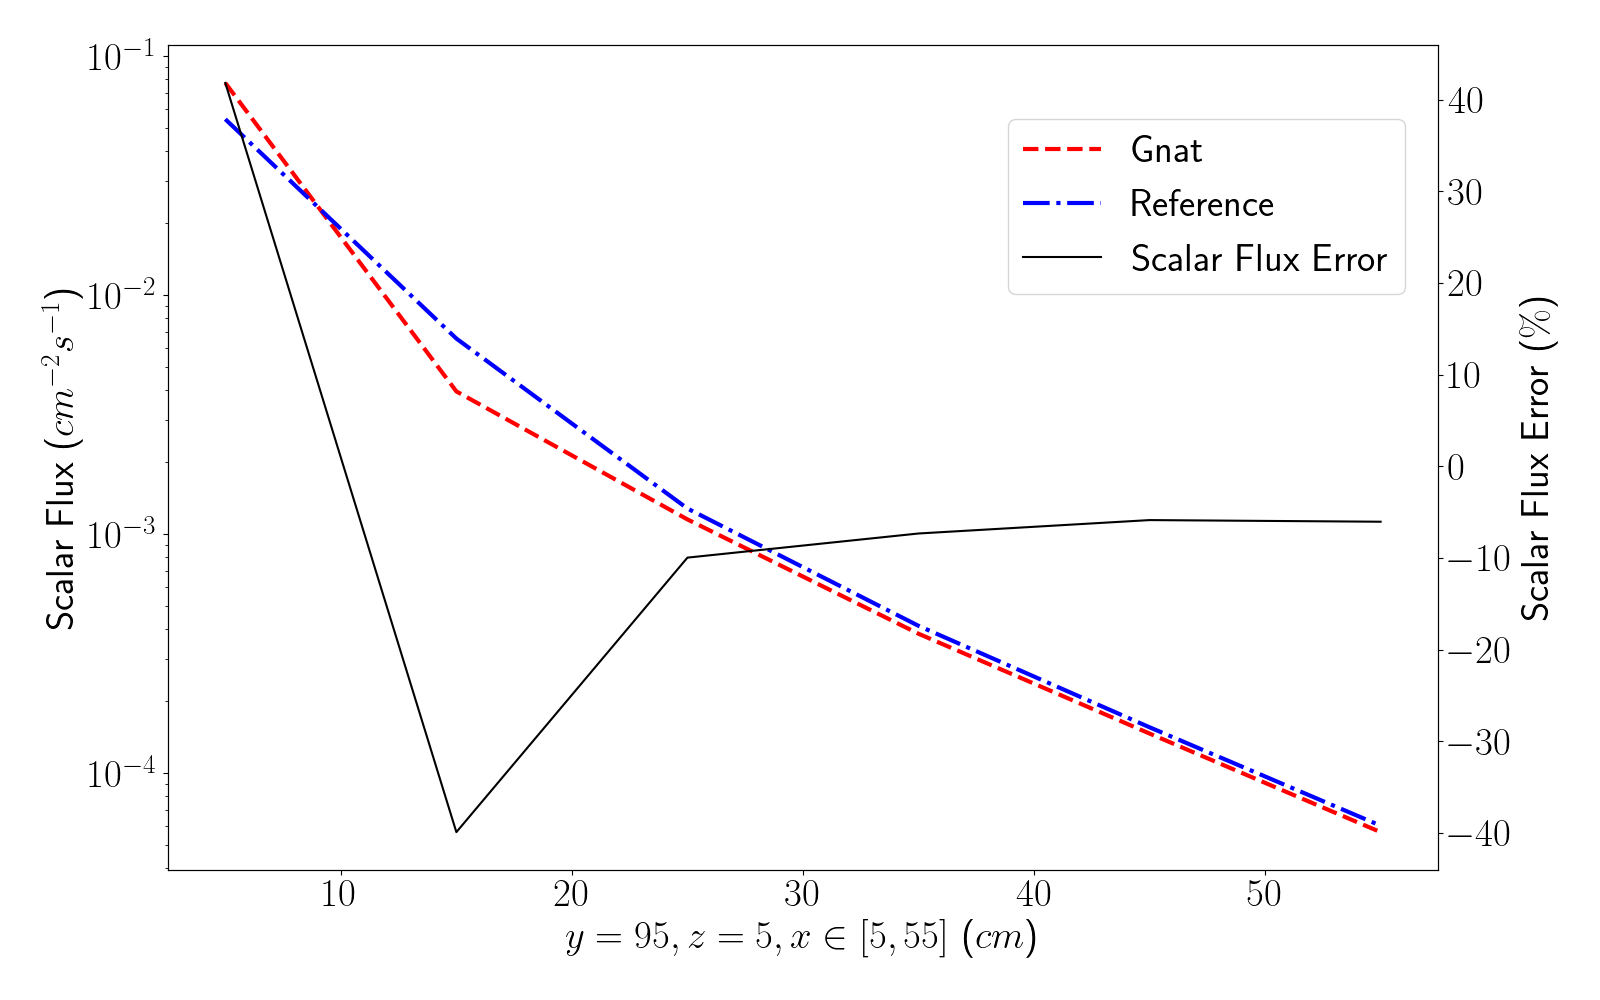
\includegraphics[width=\textwidth]{images/verification/sn_kobayashi/2/kobayashi_2b.png}
        \caption{Comparison with the benchmark problem. Reference taken from Kobayashi and Sugimura \cite{kobayashi_benchmarks}.}
        \label{fig:verification:sn_kobayashi_2b:line_plot}
    \end{subfigure}
    \caption{Results of the Kobayashi benchmark 2b.}
    \label{fig:verification:sn_kobayashi_2b}
\end{figure}

The results for the third benchmark problem can be found in Figures~\ref{fig:verification:sn_kobayashi_3a} to \ref{fig:verification:sn_kobayashi_3c}. This duct problem contains both a long streaming penetration which is prone to ray effects and several changes in the direction of the duct which requires scattering to be well resolved in the angular domain. Similar behavior to the second benchmark problem can be found in this third problem; Figure~\ref{fig:verification:sn_kobayashi_3a:line_plot} shows an increase in error along the duct due to an insufficiently resolved angular domain. This behavior changes as the scalar flux approaches the first turn in the duct; the error starts to decrease due to the influence of isotropic scattering from the shield, which the first straight-line segment of the duct terminates at. Plotting the scalar flux along the width of the duct in Figure~\ref{fig:verification:sn_kobayashi_3b:line_plot} shows a similar trend in error when compared the second benchmark (Figure~\ref{fig:verification:sn_kobayashi_2b:line_plot}). It is less severe in this case as the the line is closer to the volumetric source and scattering from the terminating shield aids in decreasing ray effects. Figure~\ref{fig:verification:sn_kobayashi_3c:line_plot} shows the scalar flux distribution within the duct after the three changes in direction. The scalar flux distribution is reasonably free of ray effects after the multiple scattering events required to pass through this deep penetration, and the most likely sources of error are the additional \acrshort{supg} stabilization added in the void region of the duct.

\begin{figure}[H]
    \centering
    \begin{subfigure}[b]{0.4\textwidth}
        \centering
        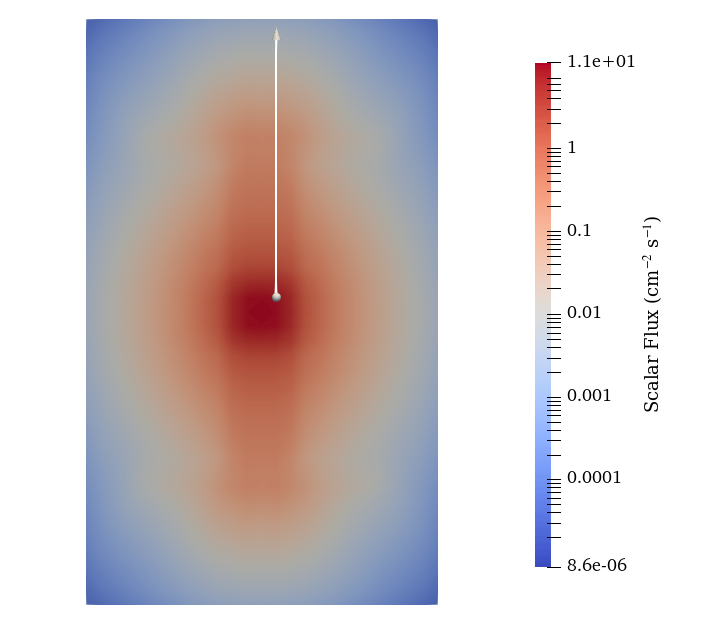
\includegraphics[width=\textwidth]{images/verification/sn_kobayashi/3/kobayashi_3a_flux_map.png}
        \caption{Scalar flux distribution associated with the line plot. The cutting plane is the x-y plane at $z = 5\text{ cm}$.}
        \label{fig:verification:sn_kobayashi_3a:flux}
    \end{subfigure}
    \hfill
    \begin{subfigure}[b]{0.59\textwidth}
        \centering
        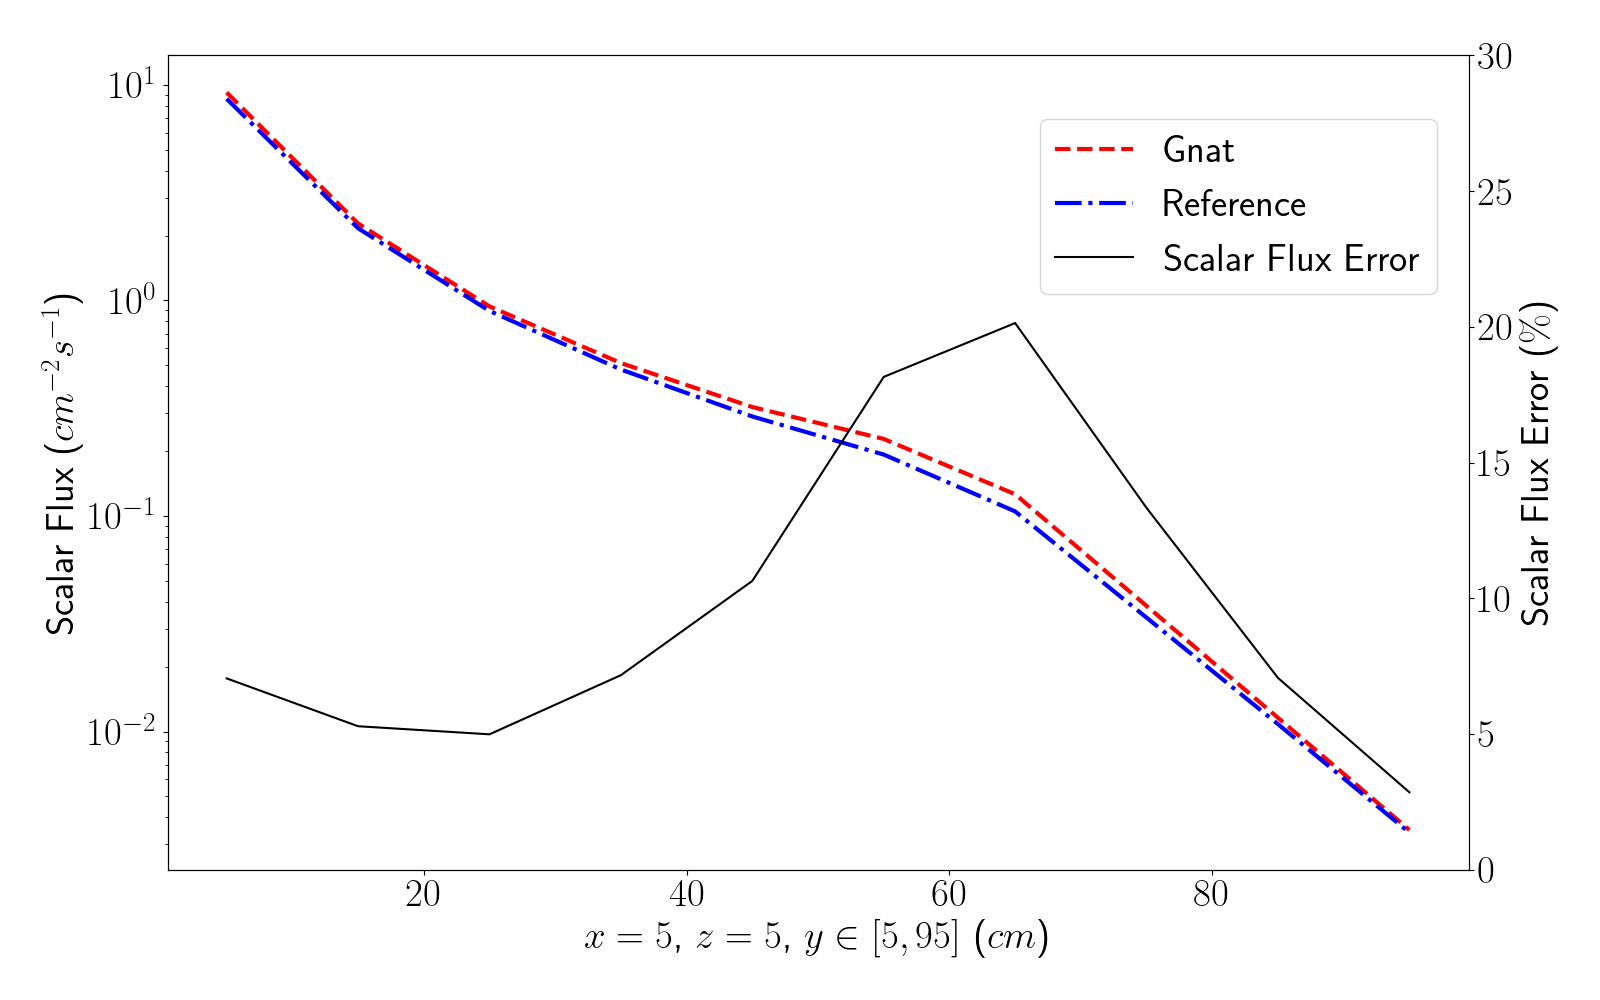
\includegraphics[width=\textwidth]{images/verification/sn_kobayashi/3/kobayashi_3a.png}
        \caption{Comparison with the benchmark problem. Reference taken from Kobayashi and Sugimura \cite{kobayashi_benchmarks}.}
        \label{fig:verification:sn_kobayashi_3a:line_plot}
    \end{subfigure}
    \caption{Results of the Kobayashi benchmark 3a.}
    \label{fig:verification:sn_kobayashi_3a}
\end{figure}

\begin{figure}[H]
    \centering
    \begin{subfigure}[b]{0.4\textwidth}
        \centering
        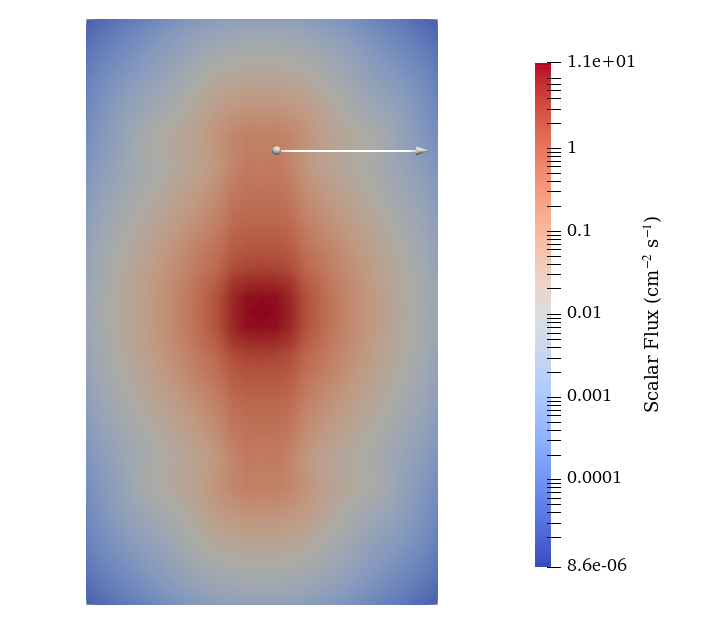
\includegraphics[width=\textwidth]{images/verification/sn_kobayashi/3/kobayashi_3b_flux_map.png}
        \caption{Scalar flux distribution associated with the line plot. The cutting plane is the x-y plane at $z = 5\text{ cm}$.}
        \label{fig:verification:sn_kobayashi_3b:flux}
    \end{subfigure}
    \hfill
    \begin{subfigure}[b]{0.59\textwidth}
        \centering
        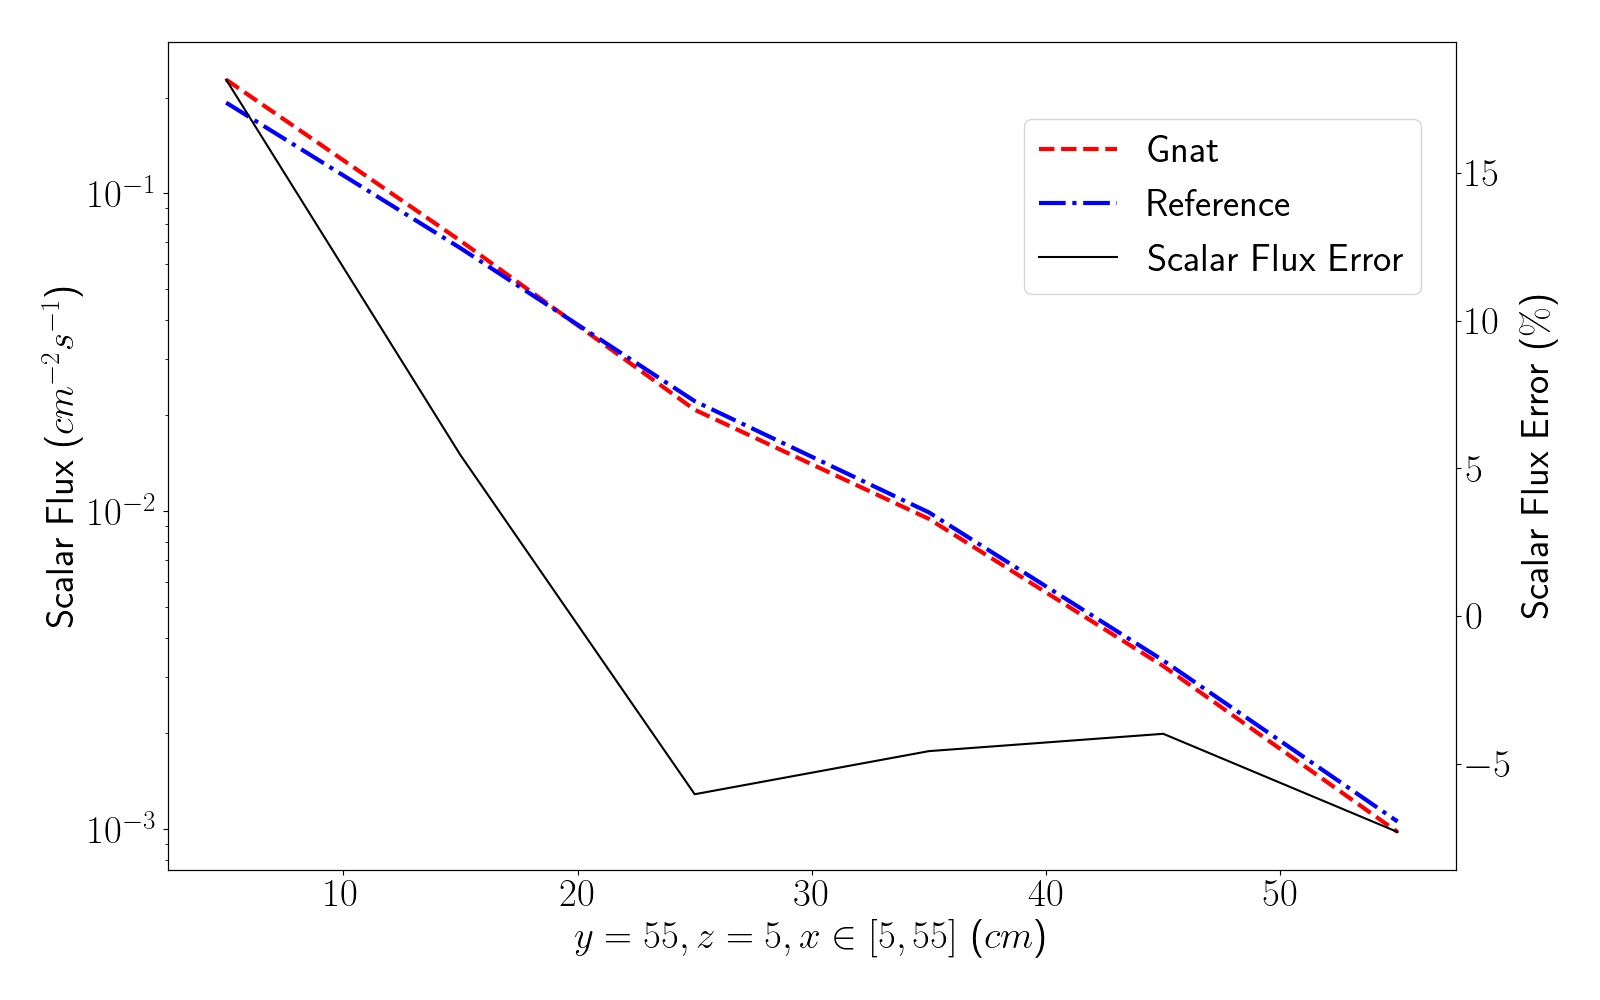
\includegraphics[width=\textwidth]{images/verification/sn_kobayashi/3/kobayashi_3b.png}
        \caption{Comparison with the benchmark problem. Reference taken from Kobayashi and Sugimura \cite{kobayashi_benchmarks}.}
        \label{fig:verification:sn_kobayashi_3b:line_plot}
    \end{subfigure}
    \caption{Results of the Kobayashi benchmark 3b.}
    \label{fig:verification:sn_kobayashi_3b}
\end{figure}

\begin{figure}[H]
    \centering
    \begin{subfigure}[b]{0.4\textwidth}
        \centering
        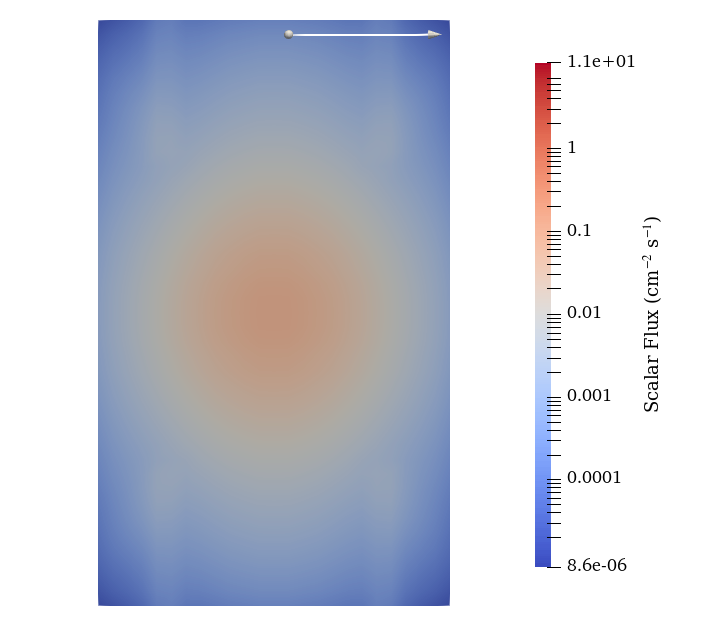
\includegraphics[width=\textwidth]{images/verification/sn_kobayashi/3/kobayashi_3c_flux_map.png}
        \caption{Scalar flux distribution associated with the line plot. The cutting plane is the x-y plane at $z = 35\text{ cm}$.}
        \label{fig:verification:sn_kobayashi_3c:flux}
    \end{subfigure}
    \hfill
    \begin{subfigure}[b]{0.59\textwidth}
        \centering
        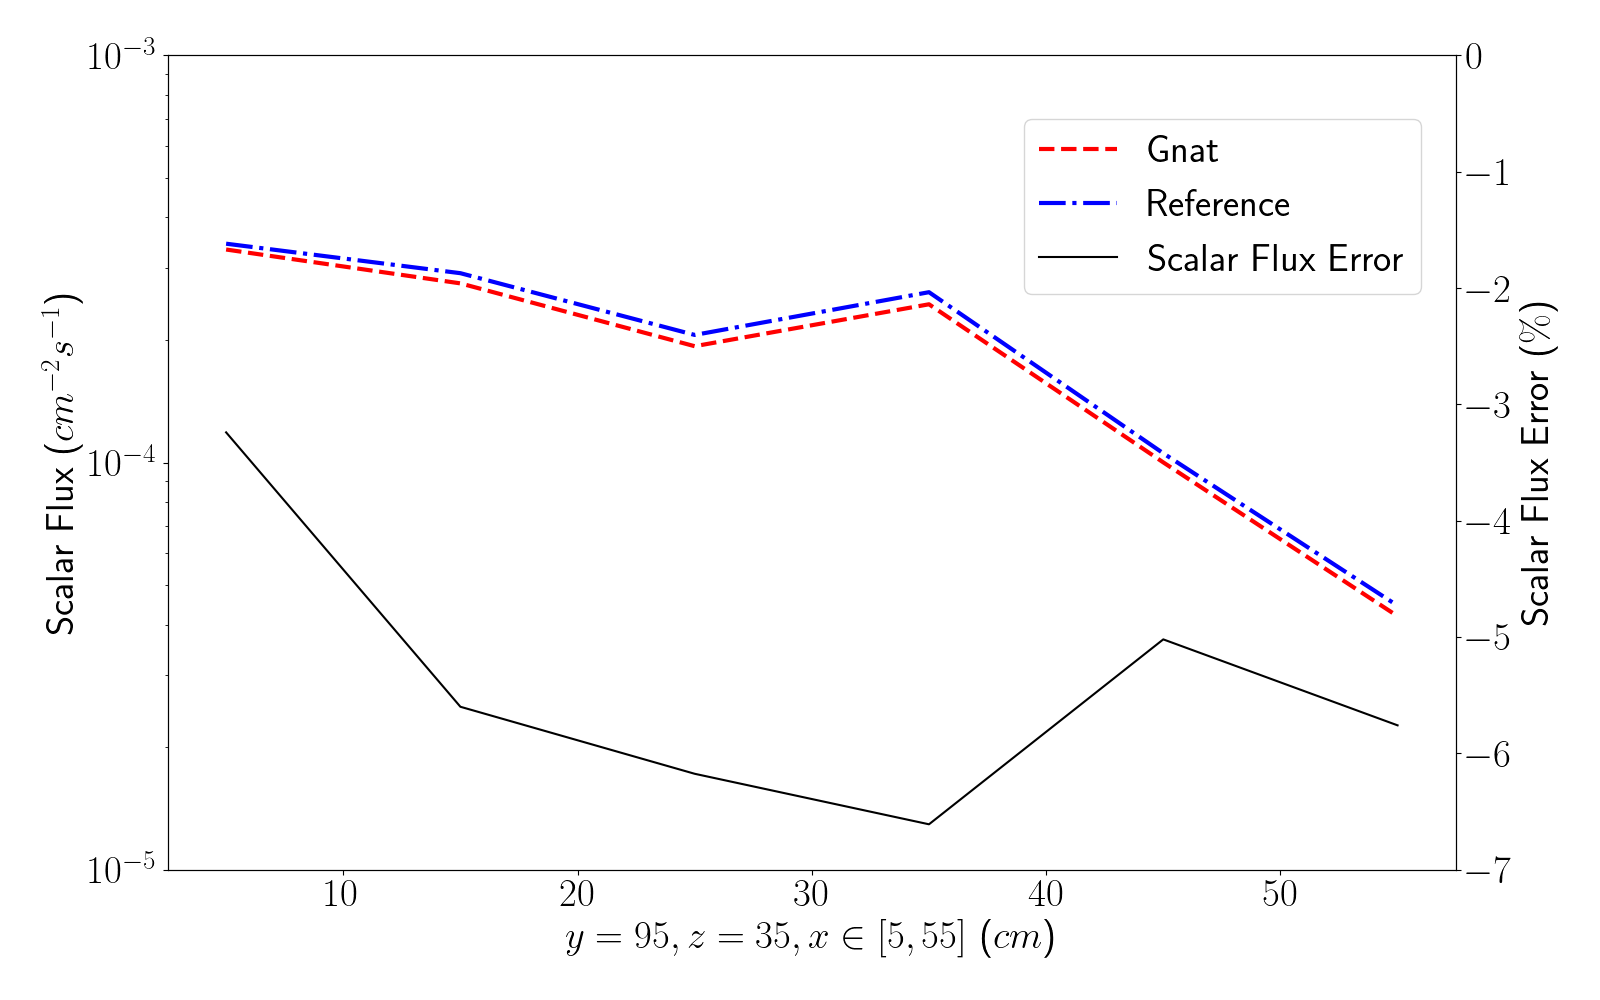
\includegraphics[width=\textwidth]{images/verification/sn_kobayashi/3/kobayashi_3c.png}
        \caption{Comparison with the benchmark problem. Reference taken from Kobayashi and Sugimura \cite{kobayashi_benchmarks}.}
        \label{fig:verification:sn_kobayashi_3c:line_plot}
    \end{subfigure}
    \caption{Results of the Kobayashi benchmark 3c.}
    \label{fig:verification:sn_kobayashi_3c}
\end{figure}

In general, the neutral particle transport solver matched the benchmark problems well. The relative error in the solutions can be explained by either a lack of a sufficiently refined spatial mesh or a need for additional angular directions to combat ray effects. The transport solver performed particularly well in optically thick diffusion regions such as the particle shield, which is expected as these regions are isotropic scattering dominant. The solver performed reasonably well when faced with jump discontinuities in cross section, however jump discontinuities which included particle sources resulted in additional error when compared with the reference solution of the first benchmark. Additional mesh refinement is considered necessary to better resolve material discontinuities in this radiation transport solver.

\subsection{The Ontario Tech Subcritical Assembly}
\label{verification:radiation_transport_sn:subcritical}

The third benchmark problem used to verify the accuracy of the \acrshort{sn} transport solver is two potential configurations of the Ontario Tech subcritical assembly \cite{ks_2024_subcritical}. These two problems were chosen for a verification study as they have to potential to be adapted to a validation benchmark in the future. The subcritical assembly is composed of $19\times 19$ square graphite elements. Each of these elements has a channel milled for either cylindrical fuel elements (natural uranium metal clad in aluminum), cylindrical graphite plugs, or cylindrical control rods (304 stainless steel). The central region of the assembly is the effective core while the remainder of the core is a reflector. The neutron sources used by the subcritical assembly consists of four americium-beryllium neutron sources with a combined intensity of $5\times 10^{7}\text{ s}^{\text{-1}}$ alongside a deuterium-tritium (D-T) neutron generator with an intensity of $1\times 10^{8}\text{ s}^{\text{-1}}$. The neutron sources are homogenized into a cube in the center of the subcritical assembly and the homogenized cross sections are assumed to be similar to that of air. The large size of the D-T neutron generator is likely to perturb the fluxes in the center of the assembly; a downside of this source homogenization is that the effects of these perturbations are not captured by this scheme. 
\begin{figure}[H]
    \centering
    \begin{subfigure}[b]{0.48\textwidth}
        \centering
        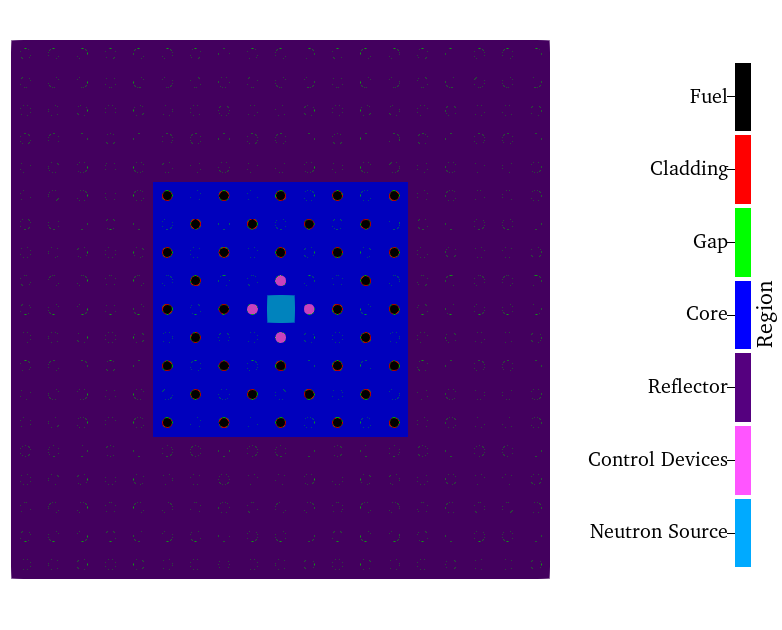
\includegraphics[width=\textwidth]{images/verification/subcritical/geo/subcritical_regions.png}
        \caption{2D lattice arrangement at $z = 0$.}
        \label{fig:subcritical_geo:2D_lattice}
    \end{subfigure}
    \hfill
    \begin{subfigure}[b]{0.48\textwidth}
        \centering
        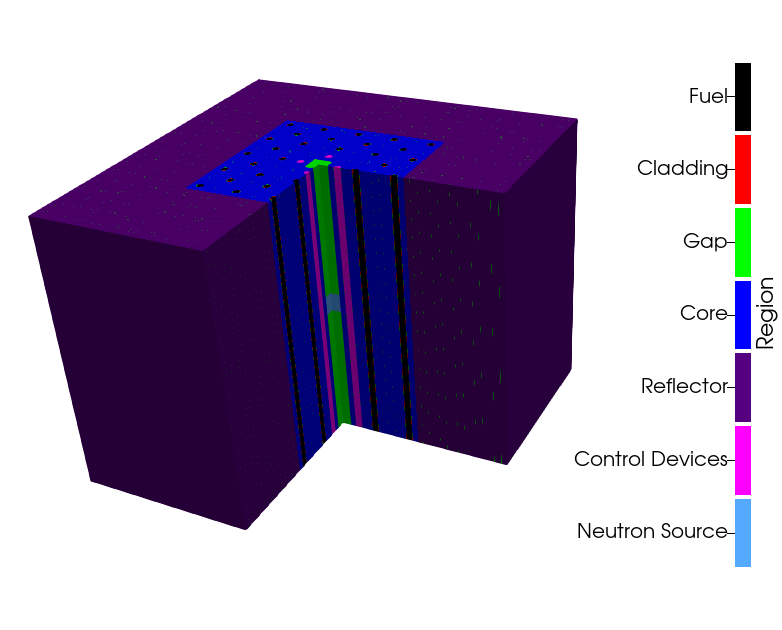
\includegraphics[width=\textwidth]{images/verification/subcritical/geo/3D_subcritical_regions.png}
        \caption{Full assembly sliced to reveal the neutron source.}
        \label{fig:subcritical_geo:full_geometry}
    \end{subfigure}
    \hfill
    \caption[The subcritical assembly benchmark geometry.]{The subcritical assembly benchmark geometry. Taken from Sawatzky and Atkinson \cite{ks_2024_subcritical}.}
    \label{fig:subcritical_geo}
\end{figure}

A lattice view of the subcritical assembly can be found in Figure~\ref{fig:subcritical_geo:2D_lattice} and a 3D view of the full core can be found in Figure~\ref{fig:subcritical_geo:full_geometry}. The first of the two subcritical assembly benchmark cases has the four control devices fully inserted. The second case has the control devices removed and replaced with graphite plugs. Both benchmark problems are criticality calculations where the eigenvalue $k_{eff}$ is the quantity of interest. The material properties of the assembly can be found in Table~\ref{table:subcritical_props} and the dimensions can be found in Figure~\ref{table:subcritical_dims}.
\begin{table}[H]
    \parbox{0.58\linewidth}
    {
        \centering
        \singlespacing
        \caption[Material properties of each region in the subcritical assembly.]{Material properties of each region in the subcritical assembly. Adapted from Sawatzky and Atkinson \cite{ks_2024_subcritical}.}
        \begin{tabular}{|c|c|c|}
            \hline
            \textbf{Region} & \makecell{\textbf{Density} \\ (g cm\textsuperscript{-3})} & \makecell{\textbf{Composition} \\(atom-fraction)}\\
            \hline
            \makecell{Fuel\\(Uranium Metal)} & $19.1$ & \makecell{\textsuperscript{235}U: $7.291\times 10^{-3}$\\\textsuperscript{238}U: $9.926\times 10^{-1}$}\\
            \hline
            \makecell{Cladding\\(Aluminum Metal)} & $2.699$ & \makecell{\textsuperscript{27}Al: $1.0$}\\
            \hline
            \makecell{Gap and \\Source\\(Air Filled)} & $1.2\times 10^{-3}$ & \makecell{\textsuperscript{14}N: $8.038\times 10^{-1}$\\\textsuperscript{15}N: $2.955\times 10^{-3}$\\\textsuperscript{16}O: $1.893\times 10^{-1}$}\\
            \hline
            \makecell{Core \& Reflector\\(Graphite)} & $1.91$ & \makecell{\textsuperscript{12}C: $9.889\times 10^{-1}$\\\textsuperscript{13}C: $1.111\times 10^{-2}$} \\
            \hline
            \makecell{Control Devices\\(304 Stainless Steel)} & $8.0$ & \makecell{\textsuperscript{12}C: $3.595\times 10^{-3}$\\\textsuperscript{28}Si: $1.792\times 10^{-2}$\\\textsuperscript{50}Cr: $9.121\times 10^{-3}$\\\textsuperscript{52}Cr: $1.759\times 10^{-1}$\\\textsuperscript{53}Cr: $1.995\times 10^{-2}$\\\textsuperscript{54}Cr: $4.965\times 10^{-3}$\\\textsuperscript{55}Mn: $1.987\times 10^{-2}$\\\textsuperscript{54}Fe: $3.761\times 10^{-2}$\\\textsuperscript{56}Fe: $5.905\times 10^{-1}$\\\textsuperscript{57}Fe: $1.363\times 10^{-2}$\\\textsuperscript{58}Fe: $1.815\times 10^{-3}$\\\textsuperscript{58}Ni: $6.963\times 10^{-2}$\\\textsuperscript{60}Ni: $2.682\times 10^{-2}$\\\textsuperscript{61}Ni: $1.166\times 10^{-3}$\\\textsuperscript{62}Ni: $3.718\times 10^{-3}$}\\
            \hline
        \end{tabular}
        \label{table:subcritical_props}
    }
    \hfill
    \parbox{0.40\linewidth}
    {
        \centering
        \singlespacing
        \caption[Dimensions of each region.]{Dimensions of each region. Adapted from Sawatzky and Atkinson \cite{ks_2024_subcritical}.}
        \begin{tabular}{|cc|}
            \hline
            \textbf{Dimension} & \textbf{Value}\\
            \hline
            Fuel Pin Diameter & $3.2766\text{ cm}$\\
            Cladding Thickness & $0.4064\text{ cm}$\\
            Block Length / Width & $10.16\text{ cm}$\\
            Channel Diameter & $3.96748\text{ cm}$\\
            Plug Diameter & $3.81\text{ cm}$\\
            Control Device Diameter & $3.81\text{ cm}$\\
            Assembly Height & $152.4\text{ cm}$\\
            \makecell{Homogenized Source \\ Length / Width / Height} & $10.16\text{ cm}$\\
            \makecell{Source Insertion Depth \\ (Top to Source Center)} & $71.12\text{ cm}$\\
            \hline
        \end{tabular}
        \label{table:subcritical_dims}
    }
\end{table}
\begin{table}[H]
    \singlespacing
    \centering
    \caption[Group structures used to generate multi-group cross sections for the subcritical assembly.]{Group structures used to generate multi-group cross sections for the subcritical assembly. Adapted from Agosta \cite{agosta_htgr}.}
    \begin{tabular}{|c|cccccccccccc|}
        \hline
          & \multicolumn{12}{c|}{}\\
         \makecell{\textbf{Upper Energy} \\ \textbf{Bound (eV)}} & \multicolumn{12}{c|}{\textbf{Group Structure}}\\
          & 26 & 21 & 18 & 15a & 15b & 15c & 15d & 15e & 12 & 9 & 6 & 3\\
         \hline
         $1.49\times 10^{7}$  & 1  & 1  & 1  & 1  & 1  & 1  & 1  & 1  & 1  & 1 & 1 & 1\\
         $7.41\times 10^{6}$  & 2  &    &    &    &    &    &    &    &    &   &   &  \\
         $3.68\times 10^{6}$  & 3  & 2  & 2  & 2  & 2  & 2  & 2  & 2  & 2  &   &   &  \\
         $6.72\times 10^{5}$  & 4  &    &    &    &    &    &    &    &    &   &   &  \\
         $1.11\times 10^{5}$  & 5  & 3  & 3  & 3  & 3  & 3  & 3  & 3  & 3  & 2 & 2 & 2\\
         $1.93\times 10^{4}$  & 6  & 4  & 4  & 4  & 4  &    &    &    & 4  &   &   &  \\
         $3.35\times 10^{3}$  & 7  &    &    &    &    &    &    &    &    &   &   &  \\
         $1.58\times 10^{3}$  & 8  & 5  & 5  &    &    & 4  &    &    &    &   &   &  \\
         $7.48\times 10^{2}$  & 9  & 6  & 6  & 5  & 5  &    & 4  & 4  & 5  & 3 &   &  \\
         $2.75\times 10^{2}$  & 10 & 7  & 7  & 6  & 6  & 5  &    &    & 6  & 4 &   &  \\
         $1.30\times 10^{2}$  & 11 & 8  & 8  & 7  & 7  &    & 5  & 5  & 7  & 5 & 3 &  \\
         $6.14\times 10^{1}$  & 12 & 9  &    &    & 8  & 6  &    &    &    &   &   &  \\
         $2.90\times 10^{1}$  & 13 & 10 & 9  & 8  & 9  &    & 6  &    &    &   &   &  \\
         $1.37\times 10^{1}$  & 14 & 11 & 10 & 9  &    &    &    &    & 8  & 6 &   &  \\
         $8.32\times 10^{0}$  & 15 & 12 & 11 & 10 & 10 & 7  & 7  & 7  & 9  &   &   &  \\
         $5.04\times 10^{0}$  & 16 &    &    &    &    &    &    &    &    &   &   &  \\
         $2.38\times 10^{0}$  & 17 & 13 & 12 & 11 & 11 & 8  & 8  & 8  & 10 & 7 & 4 & 3\\
         $1.29\times 10^{0}$  & 18 & 14 &    &    &    &    &    &    &    &   &   &  \\
         $6.50\times 10^{-1}$ & 19 & 15 & 13 & 12 & 12 & 9  & 9  & 9  & 11 & 8 & 5 &  \\
         $3.50\times 10^{-1}$ & 20 & 16 &    &    &    & 10 & 10 &    &    &   &   &  \\
         $2.00\times 10^{-1}$ & 21 & 17 & 14 & 13 & 13 & 11 & 11 & 10 &    &   &   &  \\
         $1.20\times 10^{-1}$ & 22 &    &    &    &    &    &    & 11 &    &   &   &  \\
         $8.00\times 10^{-2}$ & 23 & 18 & 15 & 14 & 14 & 12 & 12 & 12 &    &   &   &  \\
         $5.00\times 10^{-2}$ & 24 & 19 & 16 &    &    & 13 & 13 & 13 &    &   &   &  \\
         $2.00\times 10^{-2}$ & 25 & 20 & 17 & 15 & 15 & 14 & 14 & 14 & 12 & 9 & 6 &  \\
         $1.00\times 10^{-2}$ & 26 & 21 & 18 &    &    & 15 & 15 & 15 &    &   &   &  \\
         \hline
    \end{tabular}
    \label{table:subcritical_group_bnds}
\end{table}
The material properties and dimensions presented above were used to generate a model of the subcritical assembly in \texttt{OpenMC} \cite{openmc} for the purpose of generating multi-group cross sections for use with \acrshort{gnat} \cite{ks_2024_subcritical}. Agosta \cite{agosta_htgr} performed a literature view of multi-group cross section boundaries used for graphite moderated reactor systems, all of which will be used to generated cross sections for the subcritical assembly for the purposes of verifying \acrshort{gnat}. A summary of these group boundaries used can be found in Table~\ref{table:subcritical_group_bnds}. The \texttt{OpenMC} simulations used to generate the multi-group cross sections used 5,000 particles per generation, 10 generations per batch, 550 active batches and 50 inactive batches. This was sufficient to converge the fission source and reduce the standard deviations of the multi-group cross sections below 1\% \cite{ks_2024_subcritical}. These multi-group cross sections were then used with the multi-group mode of \texttt{OpenMC} to calculate the reference values of $k_{eff}$ that the \acrshort{sn} solver will be compared to, the results of which can be found in Sawatzky and Atkinson \cite{ks_2024_subcritical}.

The subcritical assembly benchmarks were meshed with 33,340 mixed tetrahedral and quadrilateral elements using the \acrshort{moose} \texttt{Reactor} module \cite{moose_reactor}. The mesh was split along three lines of symmetry: the x-y plane ($z = 0\text{cm}$), x-z plane ($y = 0\text{cm}$) and y-z plane ($x = 0\text{cm}$); this reduced the number of required elements and resulted in a 1/8\textsuperscript{th} core. Reflective boundary conditions are applied along these lines of symmetry to emulate the effect of the full assembly and vacuum boundary conditions are applied elsewhere. The resulting mesh is shown in Figure~\ref{table:subcritical_mesh}. 
\begin{figure}[H]
    \centering
    \begin{subfigure}[b]{0.48\textwidth}
        \centering
        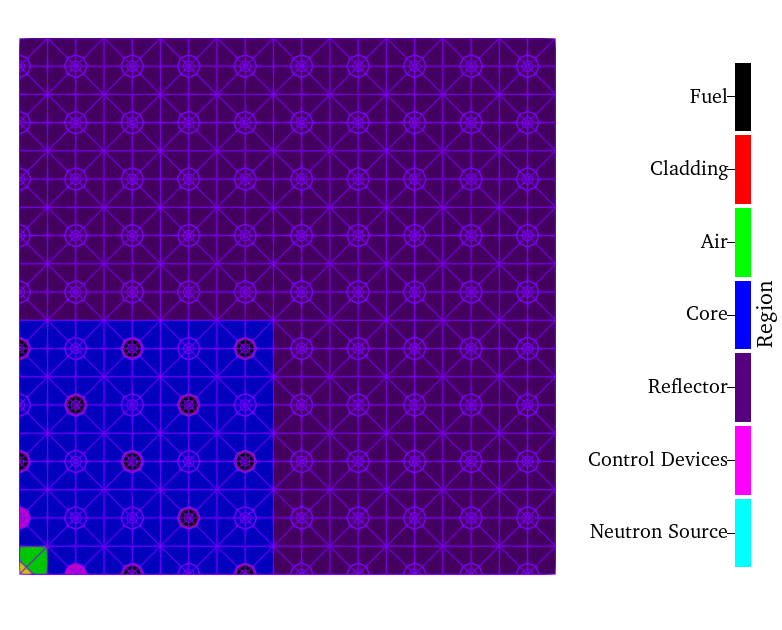
\includegraphics[width=\textwidth]{images/verification/subcritical/mesh/mesh_top.png}
        \caption{Top view of the generated mesh.}
        \label{table:subcritical_mesh_top}
    \end{subfigure}
    \hfill
    \begin{subfigure}[b]{0.48\textwidth}
        \centering
        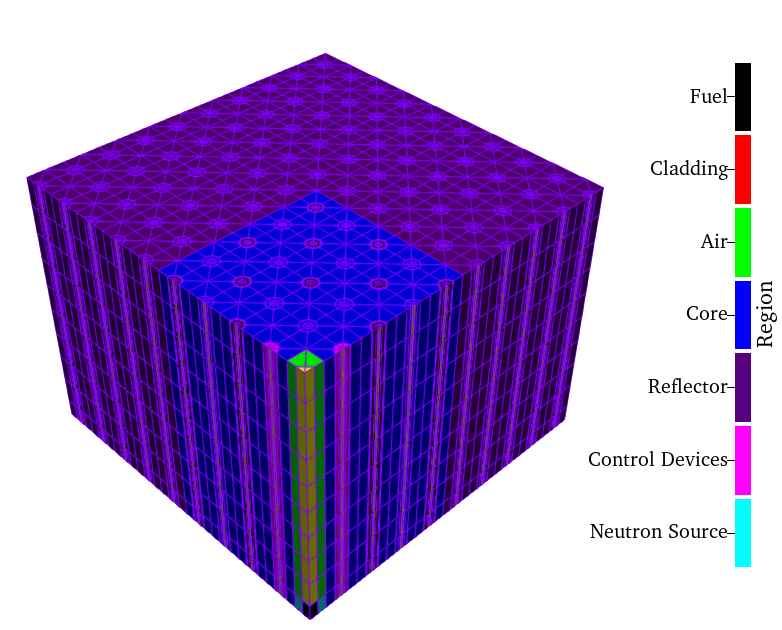
\includegraphics[width=\textwidth]{images/verification/subcritical/mesh/mesh_iso.png}
        \caption{Full view of the 1/8\textsuperscript{th} core.}
        \label{table:subcritical_mesh_iso}
    \end{subfigure}
    \hfill
    \caption[Meshed subcritical assembly geometry.]{Meshed subcritical assembly geometry. Taken from Sawatzky and Atkinson \cite{ks_2024_subcritical}.}
    \label{table:subcritical_mesh}
\end{figure}
\noindent Linear Lagrange finite element basis functions were used. All benchmark cases used the \acrshort{moose} \texttt{Eigenvalue} solver with the \acrshort{pjfnk} method using 600 \acrshort{gmres} vectors, preconditioning was provided by the hypre package BoomerAMG. Each simulation used a Gauss-Chebyshev quadrature with three polar angles and three azimuthal angles; this was considered appropriate as graphite moderated systems tend to be diffuse over the majority of the energy spectrum and do not exhibit strong streaming effects \cite{ks_2024_subcritical}. In addition to the angular resolution of the problem, the scattering anisotropy must also be considered. Transport corrected isotropic scattering cross sections were found to be as accurate as linear anisotropic scattering cross sections for this assembly, and increases in the degree of anisotropy was not found to significantly improve the accuracy of $k_{eff}$ calculations \cite{ks_2024_subcritical}. Evaluating the scattering kernel requires less computing time when isotropic scattering is assumed, and so transport corrected scattering cross sections are selected for this problem. Finally, an initial residual vector magnitude of $1.000105$ was reported by \acrshort{petsc}. This led to the use of a relative convergence criteria of $10^{-8}$ to ensure that the magnitude of the final residual vector was below $10^{-8}$ on convergence. Testing with the three group problem indicated that additional tightening of the relative convergence criteria was not required. The results of these criticality calculations alongside the absolute difference with the multi-group Monte Carlo results obtained by Sawatzky and Atkinson \cite{ks_2024_subcritical} can be found in Table~\ref{table:k_eff_gnat_vs_mc}, where $\Delta k_{eff} =  (k_{eff, \text{OpenMC}} - k_{eff, \text{Gnat}})\times 10^{-5}$ (pcm).
\begin{table}[H]
    \singlespacing
    \centering
    \caption{$k_{eff}$ predicted by \acrshort{gnat} vs multi-group \texttt{OpenMC} for both the rodded and unrodded assembly.}
    \begin{tabular}{|c|cccc|}
        \hline
        & \multicolumn{2}{c}{\textbf{Rodded Case}} & \multicolumn{2}{c|}{\textbf{Unrodded Case}}\\
        \textbf{G} & Gnat $k_{eff}$ & \makecell{$\Delta k_{eff}$ \\ (pcm)} & Gnat $k_{eff}$ & \makecell{$\Delta k_{eff}$ \\ (pcm)}\\
        \hline
        3   & $0.671352$ & $-214.5$ & $0.724530$ & $144.3$\\
        6   & $0.665454$ & $-170.5$ & $0.719861$ & $189.3$\\
        9   & $0.663403$ & $-161.8$ & $0.718573$ & $245.0$\\
        12  & $0.660716$ & $-148.0$ & $0.716210$ & $273.9$\\
        15a & $0.659284$ & $-147.1$ & $0.714858$ & $247.1$\\
        15b & $0.659357$ & $-185.0$ & $0.714962$ & $240.2$\\
        15c & $0.659720$ & $-203.4$ & $0.714931$ & $250.9$\\
        15d & $0.659908$ & $-185.0$ & $0.715010$ & $220.2$\\
        15e & $0.660165$ & $-179.9$ & $0.715167$ & $226.0$\\
        18  & $0.658896$ & $-176.3$ & $0.714572$ & $273.2$\\
        21  & $0.658691$ & $-157.5$ & $0.714353$ & $260.4$\\
        26  & $0.654831$ & $-123.9$ & $0.710522$ & $262.5$\\
        \hline
    \end{tabular}
    \label{table:k_eff_gnat_vs_mc}
\end{table}
Table~\ref{table:k_eff_gnat_vs_mc} shows that the deterministic model solved by the \acrshort{sn} transport solver over predicts $k_{eff}$ in the rodded case and under predicts $k_{eff}$ in the unrodded case when compared to the multi-group Monte Carlo reference solution. This behavior is consistent regardless of the number of energy groups or group boundaries, indicating that this is a systematic issue with the benchmark problem as implemented. A possible cause for this discrepancy is the coarse mesh used in the deterministic simulation, alongside the low order angular quadrature set. As the \acrshort{saaf} equations are not locally conservative, a poorly resolved mesh near spatially heterogeneous regions such as the fuel and control devices will result in large changes to $k_{eff}$. Ray effects appear in the fast neutron fluxes in the numerical solution \cite{ks_2024_subcritical}, which increases $|\Delta k_{eff}|$. These ray effects are caused by the lower total cross sections in the fast neutron energy groups. Future works should include testing with a more resolved mesh and a higher order angular quadrature set to ensure that the \acrshort{sn} solver converges to the multi-group Monte Carlo results. 

\section{Ray Traced Uncollided Flux}
\label{verification:radiation_transport_rt}

This section details the verification strategy used for the ray traced uncollided flux method implemented in \acrshort{gnat}. Verification begins by determining the accuracy and rate of convergence of the method using a simple analytical transport problem. This is then followed by the third Kobayashi benchmark, which is used to determine the effectiveness of the ray effect mitigation strategy when coupled with the \acrshort{sn} transport solver.

\subsection{3D Analytical Transport Problem}
\label{verification:radiation_transport_rt:3D_anal}

Consider a 3D infinite absorbing medium with a point particle source placed at the origin ($\vec{r}_{s} = \{0,0,0\}$). The radiation transport equation for this can can be written as the following:
\begin{equation}\label{eq:3D_inf_transport}
    \hat{\Omega}\cdot\vec{\nabla}\psi(\vec{r}, \hat{\Omega}) + \Sigma_{t}\psi(\vec{r},\hat{\Omega}) = \frac{q}{4\pi}\delta(\vec{r}),\,\,\,\,x\in[-\infty, \infty],y\in[-\infty, \infty],z\in[-\infty, \infty]\text{.}
\end{equation}
The solution to this transport problem can be obtained using Green's functions, and takes the following form:
\begin{equation}
    \Phi_{a}(\vec{r}) = \frac{q e^{-\Sigma_{t}||\vec{r}||}}{4\pi ||\vec{r}||}
\end{equation}
\cite{computational_methods}. This work sets $\Sigma_{t}$ to either $0.0$ cm\textsuperscript{-1} or $0.01$ cm\textsuperscript{-1} to determine the effect of cross section on the convergence of the ray traced scalar fluxes. The size of the domain is set to either 2 cm x 2 cm x 2 cm or 2000 cm x 2000 cm x 2000 cm to determine the impact of the problem length scale on the accuracy of the solution. The mesh on which the ray tracing solution is projected on contains 8,000 elements, where each element has a sided length of 0.1 cm for the 2 cm domain and 100 cm for the 2000 cm domain. The ray tracing mesh takes the projection mesh and uniformly refines it once. Both of these meshes are uniformly refined twice to determine the impact of mesh density on the accuracy of the solution. No spatial quadrature is used when computing the average fluxes; rays are traced to the element centroid and the resulting point-wise scalar flux is then divided by the element volume. The results of this case can be found in Figure~\ref{fig:verification:rt:void} and Figure~\ref{fig:verification:rt:shield} below, where the $L_{2}$ error metric is defined as:
\begin{equation}\label{eq:l2_error_rt}
    e_{L2} = \sqrt{\int_{V}\Big(\Phi(\vec{r})- \Phi_{a}(\vec{r})\Big)^{2}\,dV}\text{,}
\end{equation}
and $h$ is the average vertex separation in all elements. 

The convergence plots below exclude a region near the point source due to the singularity in the analytical solution as $||\vec{r}||$ approaches zero. To ensure that this exclusion has no impact on the measured rate of convergence the size of the near source region was set to either 10\% of the domain, 20\% of the domain, or 50\% of the domain. It can be seen that the overall $L_{2}$ error is several orders of magnitude lower in the 2000 cm domain when compared to the 2 cm domain. This is likely due to the coarse mesh resolution of the 2000 cm domain as few elements are placed near the source. Variations in the scalar flux within this region are more rapid and are therefore more susceptible to error with the average flux approach. The exclusion of even a 10\% near source region during the calculation of the $L_{2}$ compounds this issue. The rate of convergence of this technique was obtained by performing a a linear regression on the logarithm of the $L_{2}$ error and the logarithm of the mesh-average minimum vertex separation ($h$) at each mesh refinement step. The rates of convergence can be found in the legends of Figure~\ref{fig:verification:rt:void} and Figure~\ref{fig:verification:rt:shield}; it an be seen that the rate of convergence is first-order. Harbour \cite{harbour_uncollided} determined that this is the anticipated order of convergence for this approach, and so this finding lends credibility to the implementation being correct. This rate of convergence is unaffected by the cross section of the domain, size of the domain, and the size of the near source region. The exception to this is the 2000 cm absorber, where the rate of convergence is $1.2$. This is likely due to the slow variation in the solution caused by the near-full attenuation of the point source this far removed from the origin.

% 0.495
\begin{figure}[H]
    \centering
    \begin{subfigure}[b]{\textwidth}
        \centering
        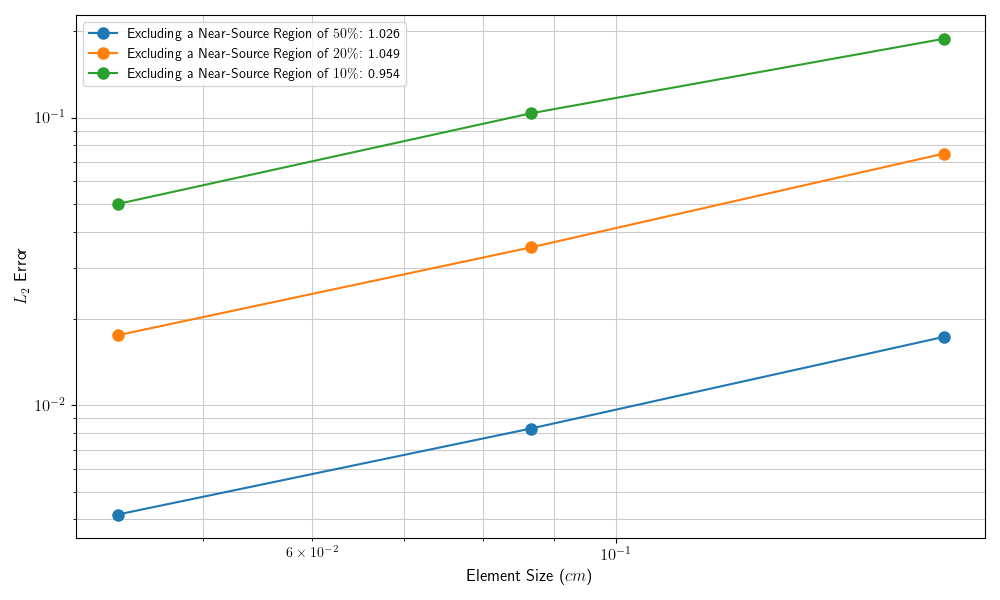
\includegraphics[width=\textwidth]{images/verification/rt_anal/vacuum_point_source_convergence_2.png}
        \caption{$L_{2}$ error for the ray traced uncollided flux technique for a 2 cm void.}
        \label{fig:verification:rt:void:2}
    \end{subfigure}
    \hfill
    \begin{subfigure}[b]{\textwidth}
        \centering
        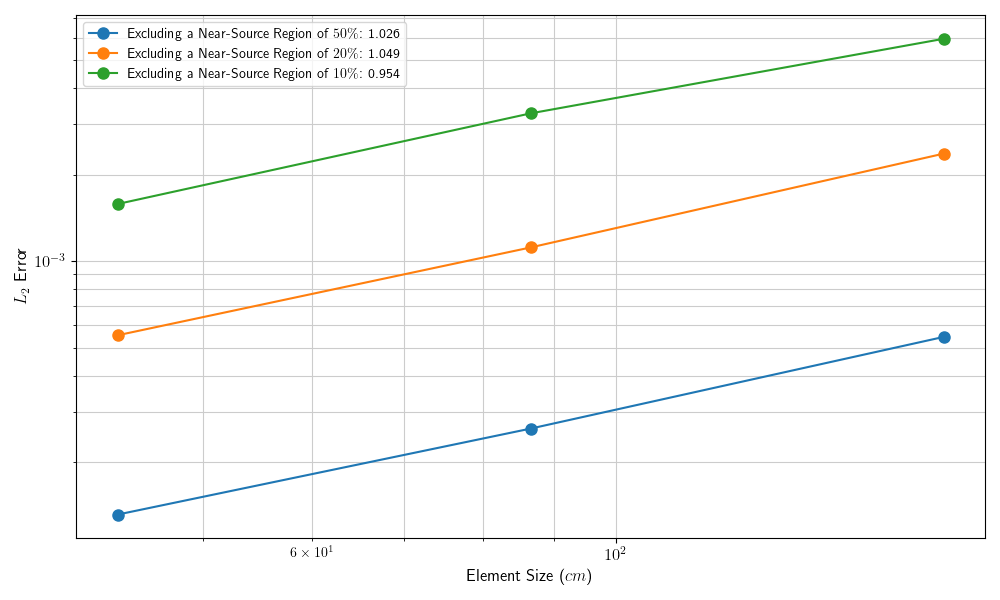
\includegraphics[width=\textwidth]{images/verification/rt_anal/vacuum_point_source_convergence_2000.png}
        \caption{$L_{2}$ error for the ray traced uncollided flux technique for a 2000 cm void.}
        \label{fig:verification:rt:void:2000}
    \end{subfigure}
    \caption{Convergence of the ray traced technique in a void.}
    \label{fig:verification:rt:void}
\end{figure}

\begin{figure}[H]
    \centering
    \begin{subfigure}[b]{\textwidth}
        \centering
        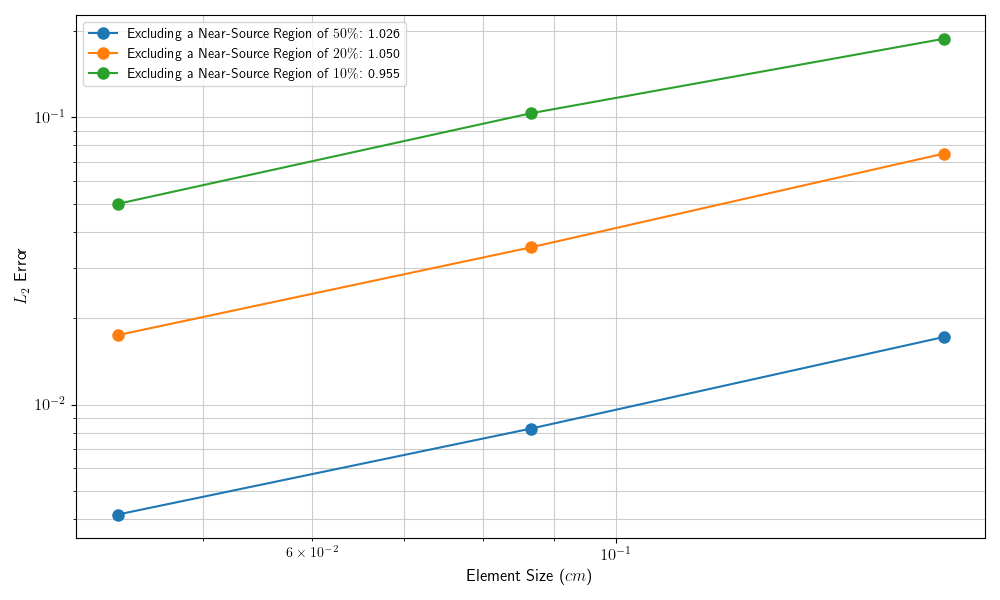
\includegraphics[width=\textwidth]{images/verification/rt_anal/shield_point_source_convergence_2.png}
        \caption{$L_{2}$ error for the ray traced uncollided flux technique for a 2 cm absorber.}
        \label{fig:verification:rt:shield:2}
    \end{subfigure}
    \hfill
    \begin{subfigure}[b]{\textwidth}
        \centering
        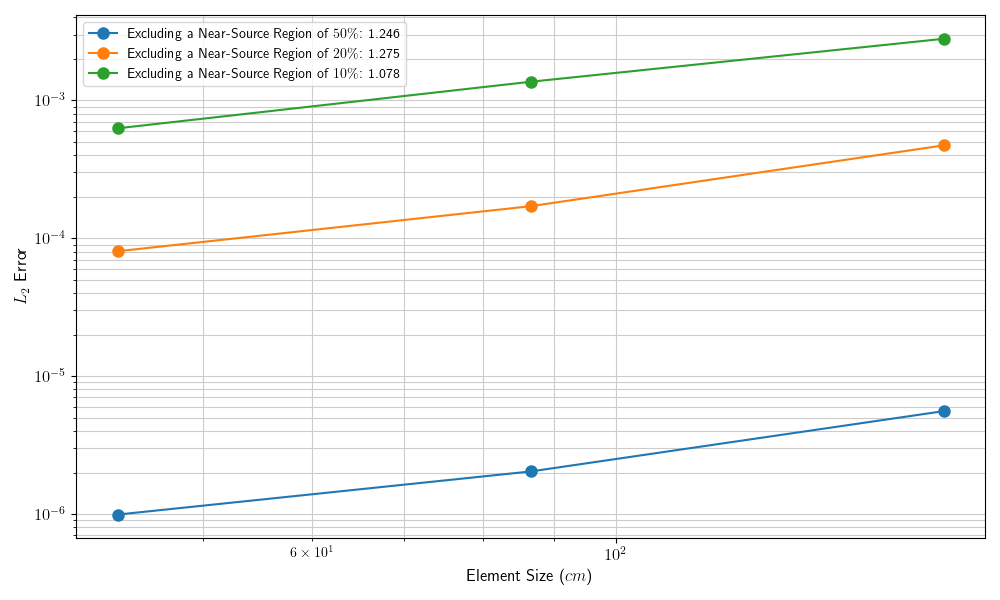
\includegraphics[width=\textwidth]{images/verification/rt_anal/shield_point_source_convergence_2000.png}
        \caption{$L_{2}$ error for the ray traced uncollided flux technique for a 2000 cm absorber.}
        \label{fig:verification:rt:shield:2000}
    \end{subfigure}
    \caption{Convergence of the ray traced technique in a light absorber.}
    \label{fig:verification:rt:shield}
\end{figure}

\subsection{The Third Kobayashi Benchmark with Ray Tracing}
\label{verification:radiation_transport_rt:kobayashi}

This verification case repeats the third Kobayashi benchmark where the ray traced uncollided flux method is used to remove ray effects. The problem is initially solved with a Gauss-Chebyshev quadrature set using 5 polar angles and 5 azimuthal angles per octant of the unit sphere, resulting in a total of 200 angular directions. The remaining parameters of the solution are the same as Section~\ref{verification:radiation_transport_rt:kobayashi}. The method of ray tracing was then used to solve for the uncollided flux, which was passed as the first collision source into the \acrshort{sn} solver to resolve the collided flux with the same angular quadrature set. The ray tracing mesh was once refined from the mesh used in Section~\ref{verification:radiation_transport_rt:kobayashi}, resulting in a total of 184,320 elements. Out of these elements, 512 contained the volumetric source. This resulted in the need to trace 94,371,328 rays from the volume sources to the non-source elements using the cell-centered approach. A Gauss-Chebyshev quadrature with 30 polar angles and 30 azimuthal angles per octant of the unit sphere was used to compute the contribution of a source element to itself. In total, this mitigation strategy required 98,057,728 rays to compute the uncollided flux. The results of this ray effect mitigation approach can be found in Figures~\ref{fig:verification:rt:kobayashi_3a} to \ref{fig:verification:rt:kobayashi_3c}.

Viewing the results below, it can be seen that this lower-order ray traced uncollided flux method is reasonably effective at removing ray effects from the third Kobayashi benchmark. Figure~\ref{fig:verification:rt:kobayashi_3a} shows how the error in the solution increases over the length of the duct up to a maximum of 10\%. The error then rapidly increases in the shielded region to -30\%. Ray effect mitigation replaces this error with a relatively constant error over the length of the duct which peaks right after the particle source and near the transition between duct and shield. This behavior is likely due to rapid variations of the scalar flux which are not well represented by the average fluxes in this numerical result. Figure~\ref{fig:verification:rt:kobayashi_3b} shows how the rapid variations in the scalar flux near the particle shield canont be accurately captured by the first order accurate uncollided flux approach, resulting in an accuracy penalty when compared to the \acrshort{sn} results. The benefits of ray effect mitigation become more apparent in Figure~\ref{fig:verification:rt:kobayashi_3c} when plotting over the duct after it undergoes several right angle turns. The ray effect mitigation approach decreases the error from a maximum of 40\% to 24\%. The distribution of the scalar flux in Figure~\ref{fig:verification:rt:kobayashi_3c:rt} more closely represents the reference solution then the scalar flux in Figure~\ref{fig:verification:rt:kobayashi_3c:no_rt}. This indicates that this low order ray effect mitigation approach is the most effective for deep penetration problems when many \acrshort{sn} directions cannot be used. In general, the ray traced solution matches the reference solution well when considering the lack of a spatial quadrature when computing the average uncollided scalar flux and the use of a coarse mesh.

\begin{figure}[H]
    \centering
    \begin{subfigure}[b]{\textwidth}
        \centering
        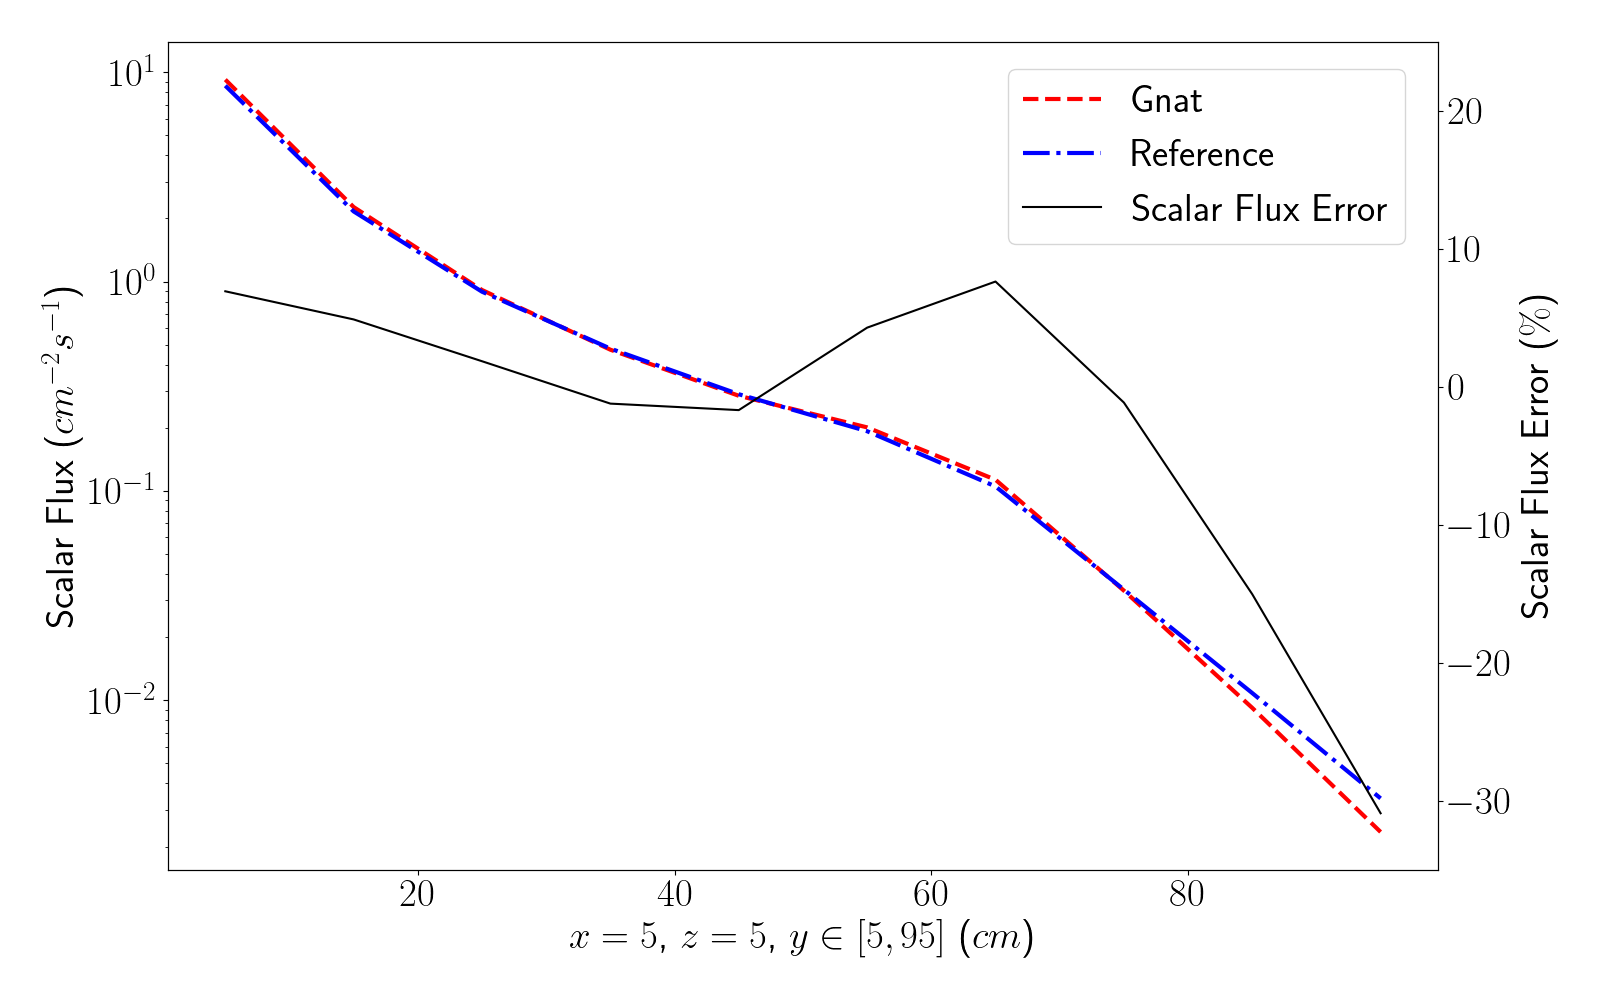
\includegraphics[width=0.8\textwidth]{images/verification/rt_kobayashi/kobayashi_3a_no_rt.png}
        \caption{No ray effect mitigation. Reference taken from Kobayashi and Sugimura \cite{kobayashi_benchmarks}.}
        \label{fig:verification:rt:kobayashi_3a:no_rt}
    \end{subfigure}
    \hfill
    \begin{subfigure}[b]{\textwidth}
        \centering
        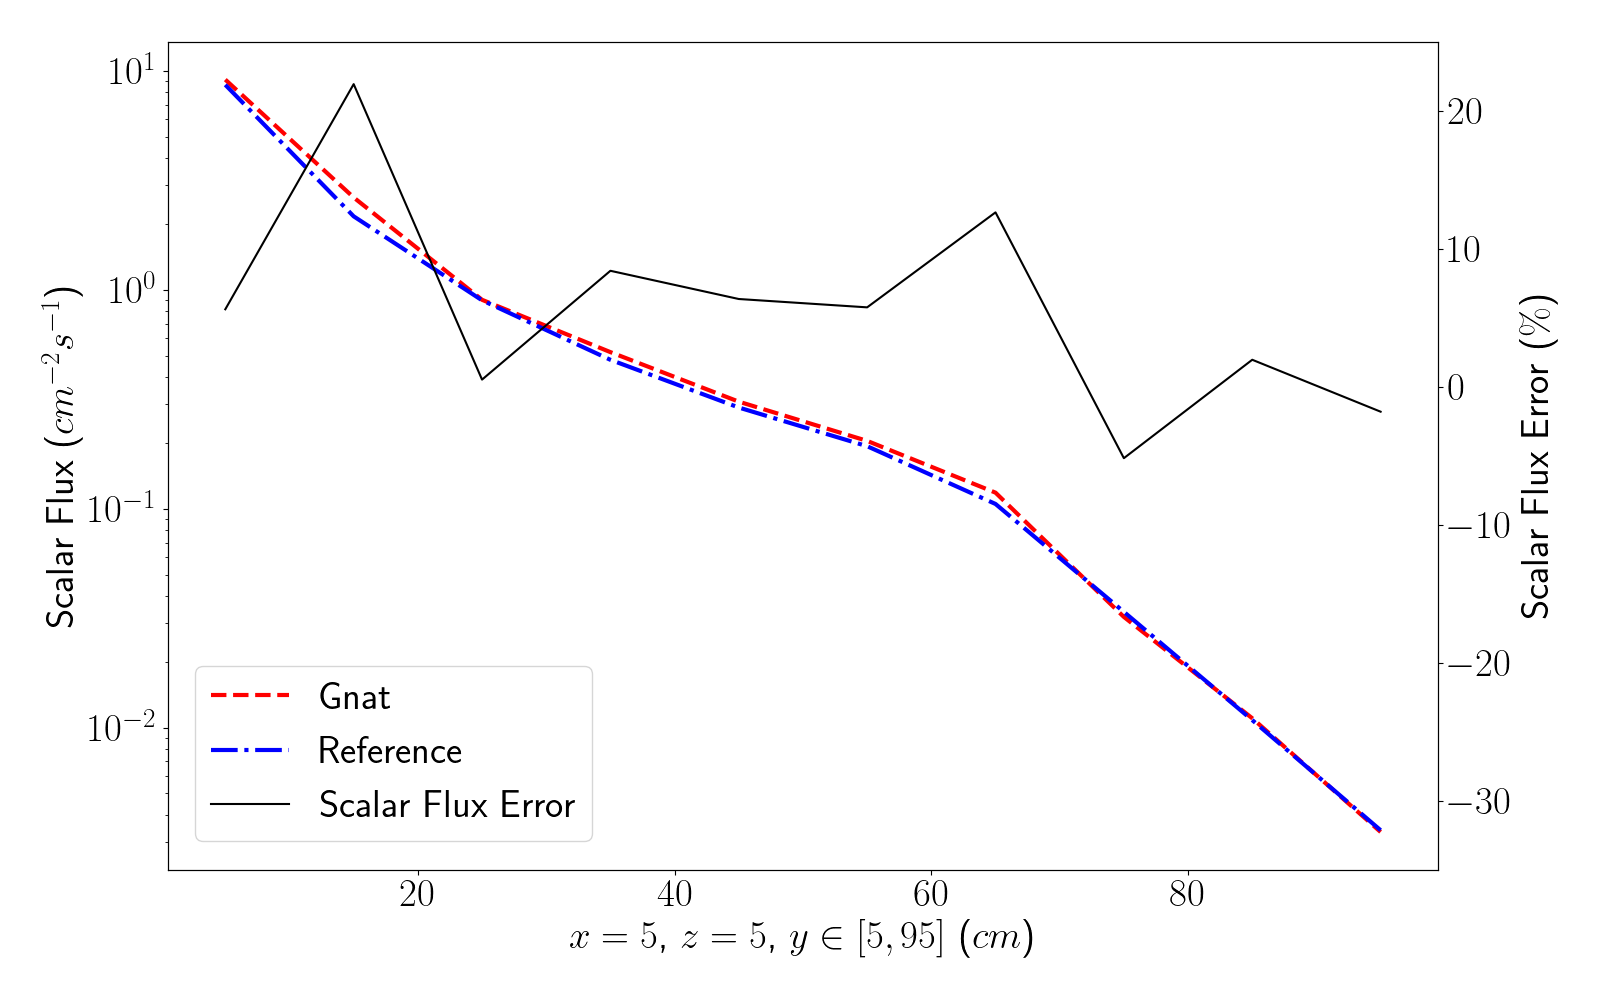
\includegraphics[width=0.8\textwidth]{images/verification/rt_kobayashi/kobayashi_3a_rt.png}
        \caption{With ray effect mitigation. Reference taken from Kobayashi and Sugimura \cite{kobayashi_benchmarks}.}
        \label{fig:verification:rt:kobayashi_3a:rt}
    \end{subfigure}
    \caption{Ray effect mitigation applied to the third Kobayashi benchmark, case a.}
    \label{fig:verification:rt:kobayashi_3a}
\end{figure}

\begin{figure}[H]
    \centering
    \begin{subfigure}[b]{\textwidth}
        \centering
        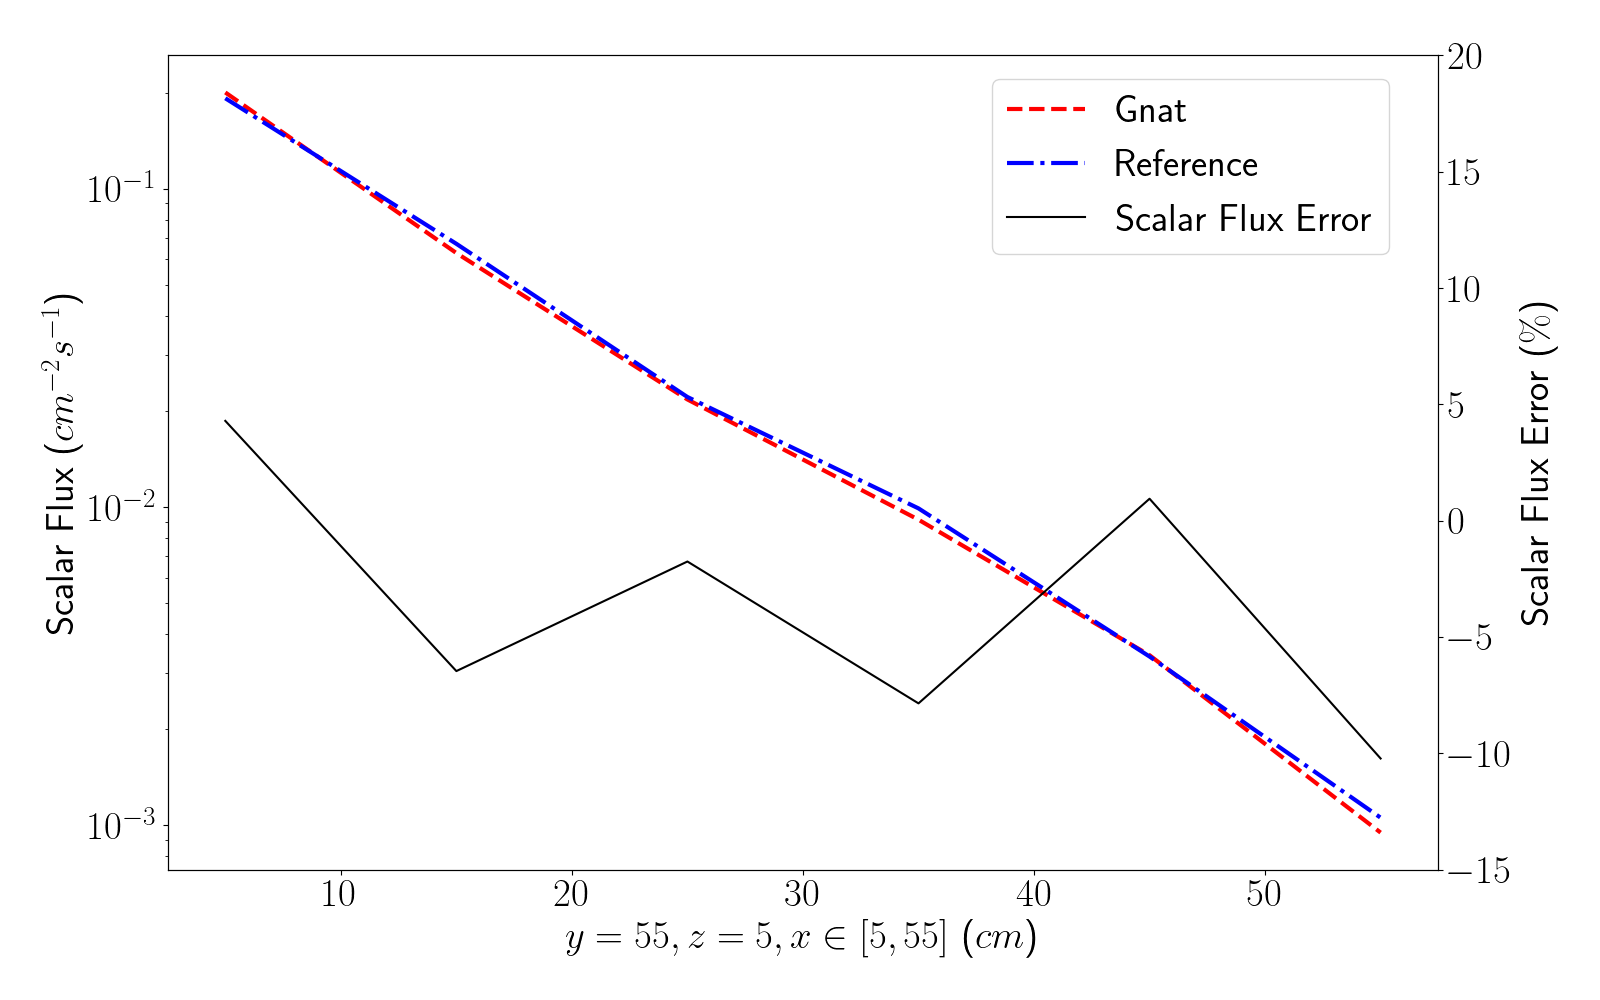
\includegraphics[width=0.8\textwidth]{images/verification/rt_kobayashi/kobayashi_3b_no_rt.png}
        \caption{No ray effect mitigation. Reference taken from Kobayashi and Sugimura \cite{kobayashi_benchmarks}.}
        \label{fig:verification:rt:kobayashi_3b:no_rt}
    \end{subfigure}
    \hfill
    \begin{subfigure}[b]{\textwidth}
        \centering
        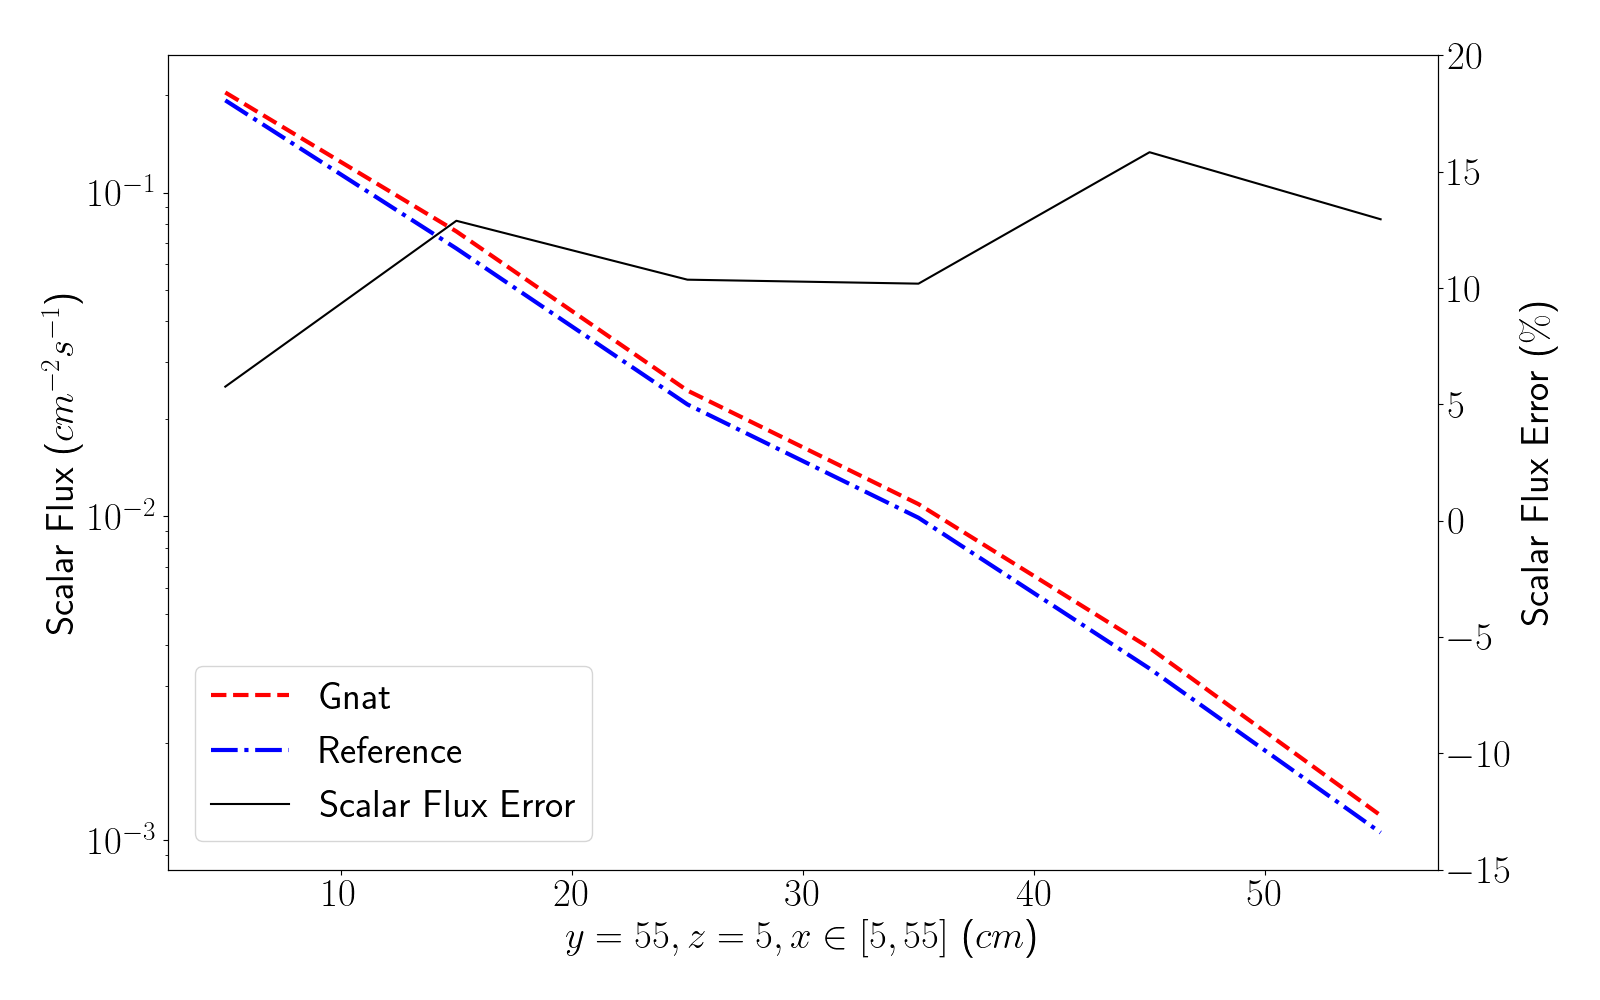
\includegraphics[width=0.8\textwidth]{images/verification/rt_kobayashi/kobayashi_3b_rt.png}
        \caption{With ray effect mitigation. Reference taken from Kobayashi and Sugimura \cite{kobayashi_benchmarks}.}
        \label{fig:verification:rt:kobayashi_3b:rt}
    \end{subfigure}
    \caption{Ray effect mitigation applied to the third Kobayashi benchmark, case b.}
    \label{fig:verification:rt:kobayashi_3b}
\end{figure}

\begin{figure}[H]
    \centering
    \begin{subfigure}[b]{\textwidth}
        \centering
        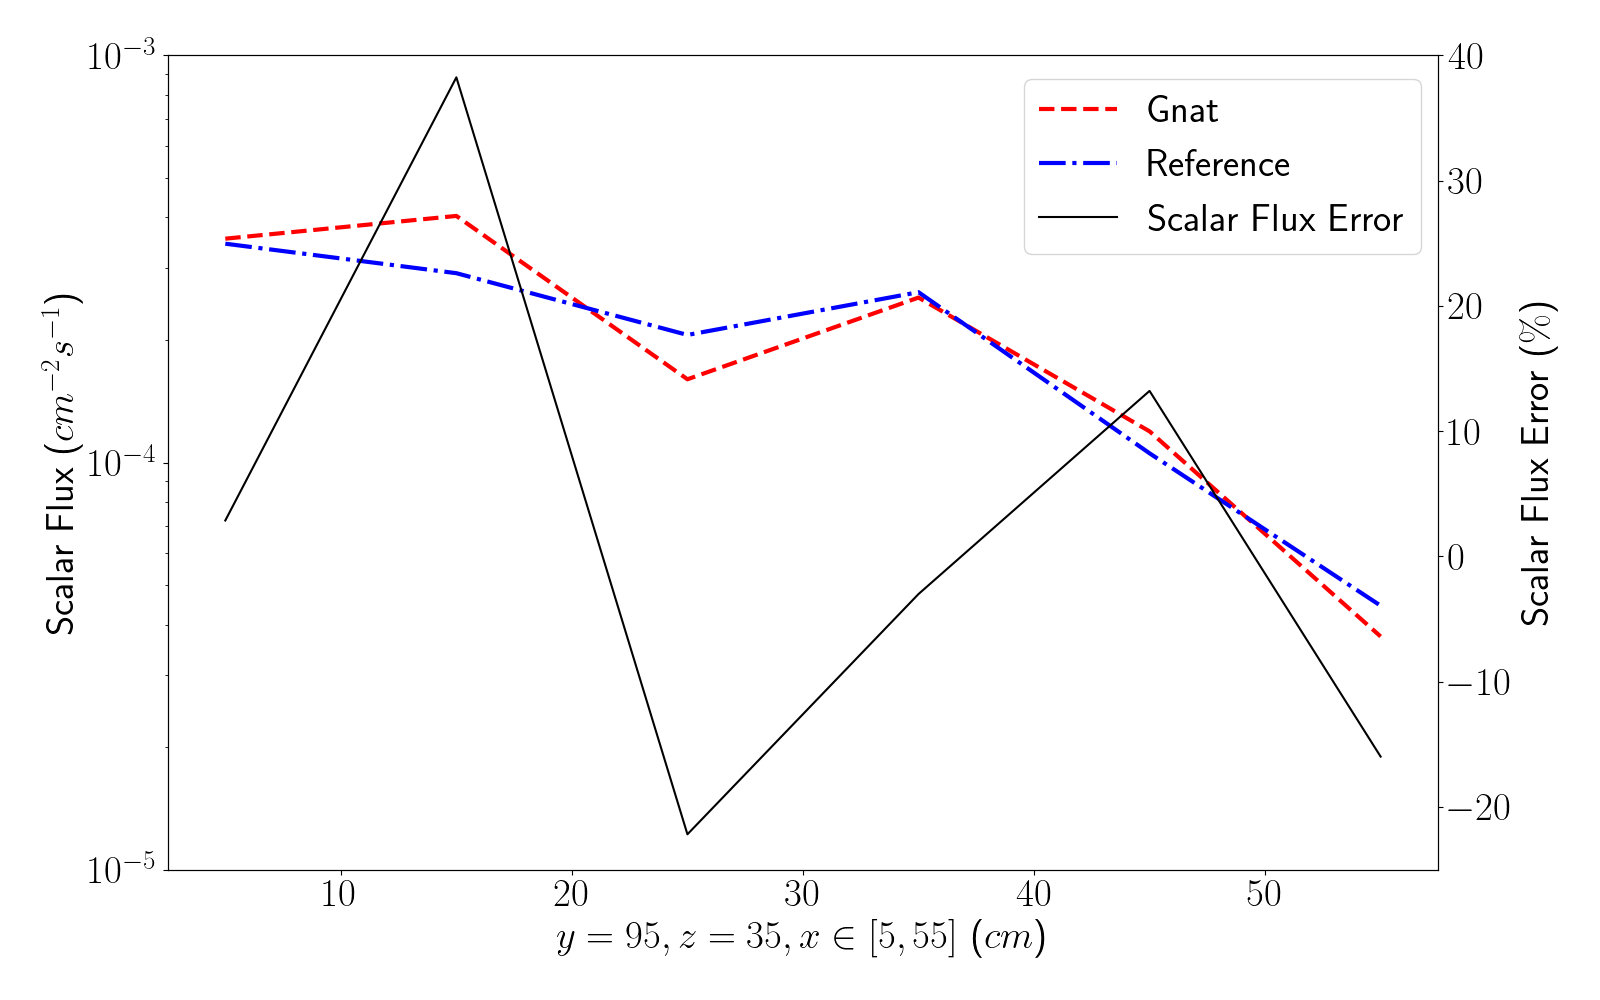
\includegraphics[width=0.8\textwidth]{images/verification/rt_kobayashi/kobayashi_3c_no_rt.png}
        \caption{No ray effect mitigation. Reference taken from Kobayashi and Sugimura \cite{kobayashi_benchmarks}.}
        \label{fig:verification:rt:kobayashi_3c:no_rt}
    \end{subfigure}
    \hfill
    \begin{subfigure}[b]{\textwidth}
        \centering
        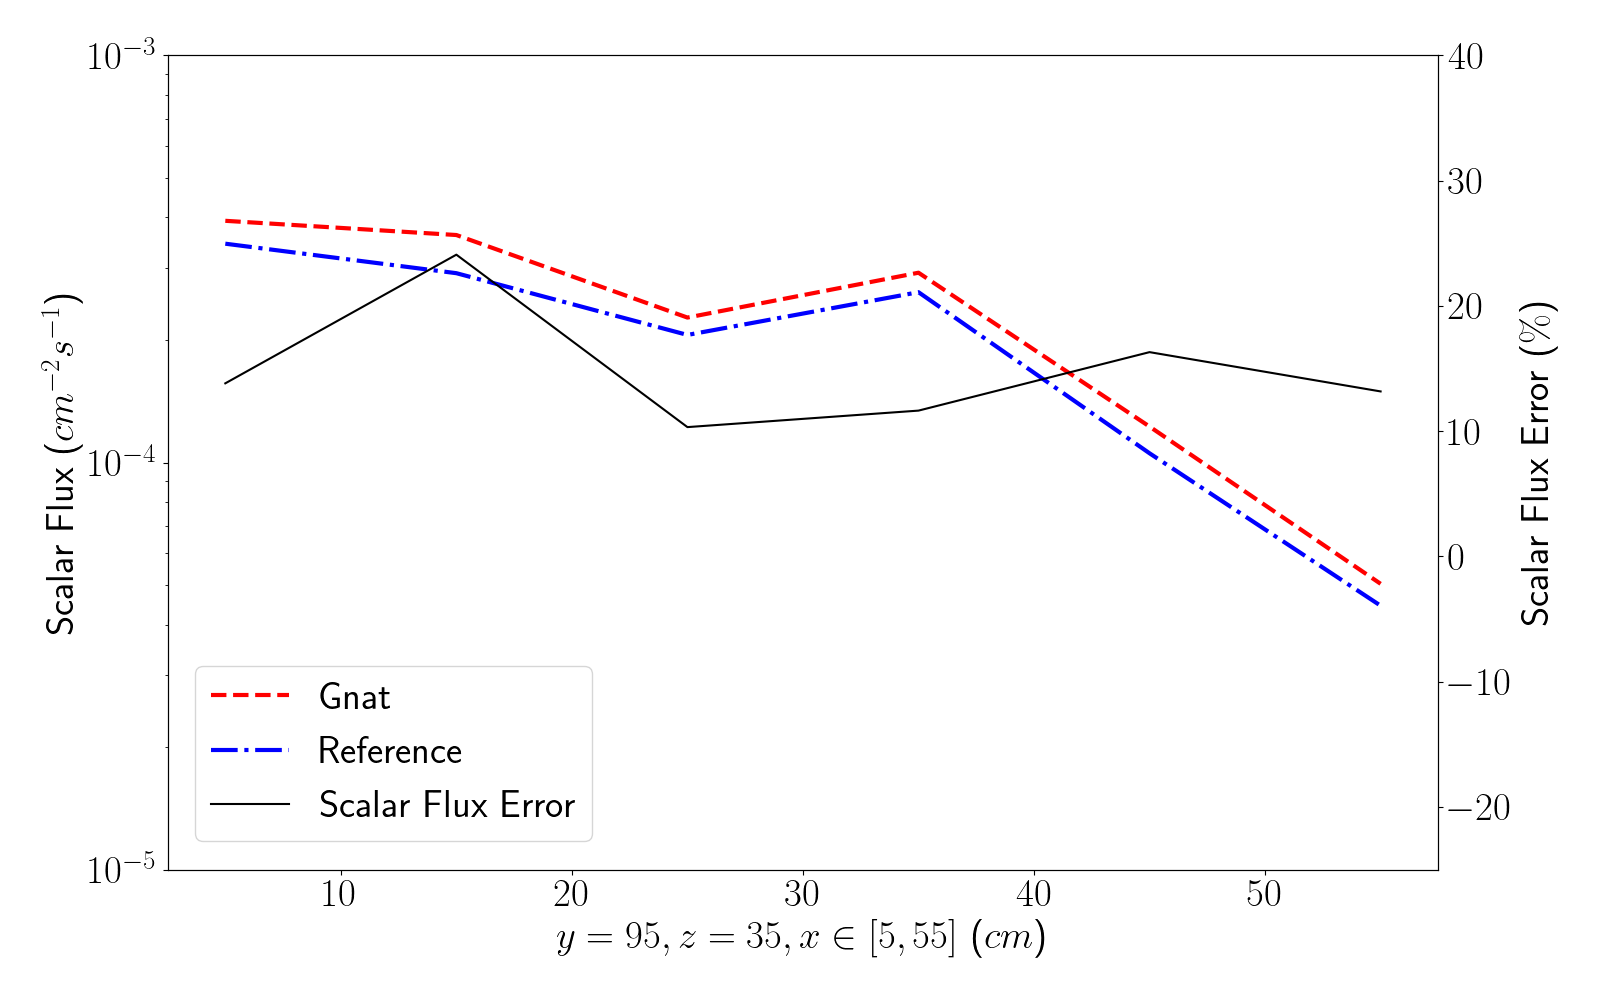
\includegraphics[width=0.8\textwidth]{images/verification/rt_kobayashi/kobayashi_3c_rt.png}
        \caption{With ray effect mitigation. Reference taken from Kobayashi and Sugimura \cite{kobayashi_benchmarks}.}
        \label{fig:verification:rt:kobayashi_3c:rt}
    \end{subfigure}
    \caption{Ray effect mitigation applied to the third Kobayashi benchmark, case c.}
    \label{fig:verification:rt:kobayashi_3c}
\end{figure}
\clearpage

\section{The Self-Adjoint Scalar Flux Approach}
\label{verification:radiation_transport_sasf}

The novel \acrshort{sasf} approach developed in this work was verified with a modified form of the third Kobayashi benchmark. The scattering cross section is set to zero to evaluate a pure absorber problem. As the \acrshort{sasf} technique does not support volumetric or surface sources the source in region one of the Kobayashi benchmark is set to zero. In its place a point source is placed at the origin with an emission rate of $1$ s\textsuperscript{-1}. As there is no existing reference solution to this problem, the method of ray tracing is used to compute scalar fluxes at the element centroids of a 1,474,560 element mesh generated with uniform cube elements. The numerical solution computed with the \acrshort{sasf} method is then sampled at the element centroids of the mesh used for ray tracing for the purposes of computing the relative error. The numerical solution to this problem is computed on a mesh with 1,641,551 nonuniform tetrahedral elements with an average $h$ of 1.131 cm. The region which previously contained the volumetric source is selected as the near-source region for the purposes of removing the singularity in the \acrshort{sasf} equation. The finite element basis functions used were linear Lagrange functions. This case used the \acrshort{pjfnk} solver with preconditioning provided by the hypre package BoomerAMG and 30 \acrshort{gmres} vectors. The initial residual vector magnitude was found to be $1.416106\times 10^{-4}$, and so a relative convergence criteria of $10^{-8}$ is required to ensure that false convergence is not reached at a final residual vector magnitude of $10^{-8}$. 

The results of this problem can be found in Figure~\ref{fig:verification:sasf:z5} for the case where $z = 5$ cm, and the results for the $z = 35$ case can be found in Figure~\ref{fig:verification:sasf:z35}. The largest sources of error occur in three locations: the edges of material discontinuities, the edges of shadows, and the edges of large streaming paths. These are mostly likely caused by large discontinuities in the gradient of the solution perpendicular to the direction of radiation. These errors are severe in this 3D case due to the complexity of the geometry and the addition of surfaces which yield jump discontinuities. Adaptive mesh refinement may be effective for mitigating these errors in problems with highly heterogeneous geometry. Aside from these sources of error the remainder of the error is largely unstructured over the domain. This is likely caused by small changes in the element density across the non-uniform mesh, yielding small fluctuations in error. In general, the numerical solution is free of ray effect and matches the reference solution quite well over the majority of the computational domain.

% 0.325
\begin{figure}[H]
    \centering
    \begin{subfigure}[b]{0.47\textwidth}
        \centering
        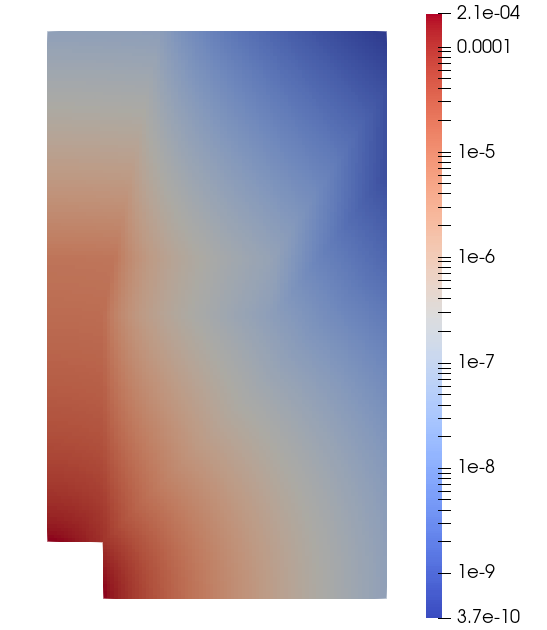
\includegraphics[width=\textwidth]{images/verification/sasf_kobayashi/rt_z5.png}
        \caption{Reference scalar flux (cm\textsuperscript{-2} s\textsuperscript{-1}).}
        \label{fig:verification:sasf:ref_z5}
    \end{subfigure}
    \hfill
    \begin{subfigure}[b]{0.47\textwidth}
        \centering
        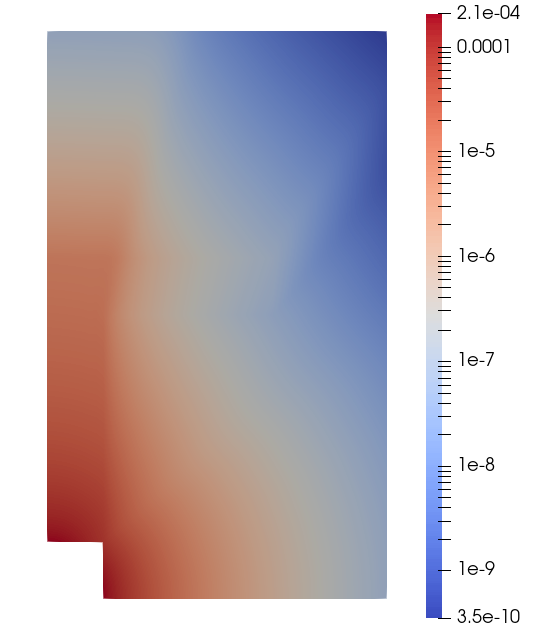
\includegraphics[width=\textwidth]{images/verification/sasf_kobayashi/sasf_z5.png}
        \caption{\acrshort{sasf} scalar flux (cm\textsuperscript{-2} s\textsuperscript{-1}).}
        \label{fig:verification:sasf:sasf_z5}
    \end{subfigure}
    \begin{subfigure}[b]{0.47\textwidth}
        \centering
        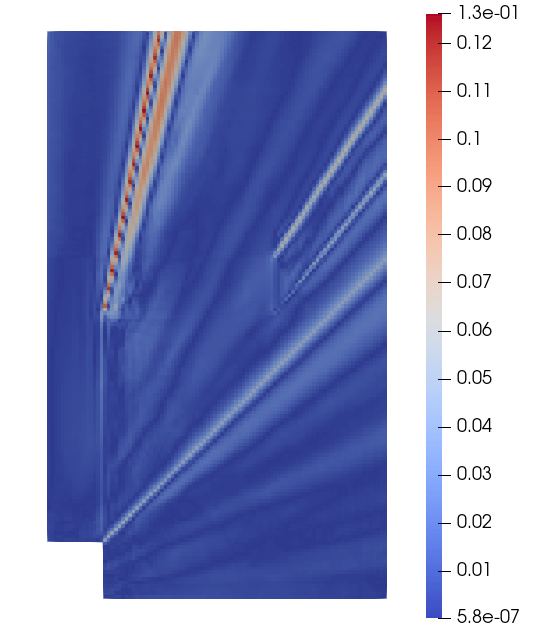
\includegraphics[width=\textwidth]{images/verification/sasf_kobayashi/error_z5}
        \caption{Fractional absolute relative error.}
        \label{fig:verification:sasf:error_z5}
    \end{subfigure}
    \caption{Comparison of scalar fluxes at $z = 5$.}
    \label{fig:verification:sasf:z5}
\end{figure}
\begin{figure}[H]
    \centering
    \begin{subfigure}[b]{0.47\textwidth}
        \centering
        \includegraphics[width=\textwidth]{images/verification/sasf_kobayashi/rt_z35.png}
        \caption{Reference scalar flux (cm\textsuperscript{-2} s\textsuperscript{-1}).}
        \label{fig:verification:sasf:ref_z35}
    \end{subfigure}
    \hfill
    \begin{subfigure}[b]{0.47\textwidth}
        \centering
        \includegraphics[width=\textwidth]{images/verification/sasf_kobayashi/sasf_z35.png}
        \caption{\acrshort{sasf} scalar flux (cm\textsuperscript{-2} s\textsuperscript{-1}).}
        \label{fig:verification:sasf:sasf_z35}
    \end{subfigure}
    \begin{subfigure}[b]{0.47\textwidth}
        \centering
        \includegraphics[width=\textwidth]{images/verification/sasf_kobayashi/error_z35}
        \caption{Fractional absolute relative error.}
        \label{fig:verification:sasf:error_z35}
    \end{subfigure}
    \caption{Comparison of scalar fluxes at $z = 35$.}
    \label{fig:verification:sasf:z35}
\end{figure}

\section{The Method of Manufactured Solutions for Mobile Depletion}
\label{verification:mms_mobile_depletion}

The \acrfull{mms} is a verification strategy for partial differential equations similar to comparisons with analytical solutions; it sees an abundance of use for problems which do not have simple analytical solutions in multiple dimensions. The \acrshort{mms} assumes a solution to the governing system of partial differential equations and then computes a forcing function which generates that assumed solution. Consider a radionuclide in a 2D domain under the influence of advection, diffusion, and radioactive decay:
\begin{align}\label{eq:simple_depletion}
    \frac{\partial}{\partial t}N(x,y,t) + \lambda_{i}N(x,y,t) + v_{x}\frac{\partial}{\partial x}N(x,y,t) + v_{y}\frac{\partial}{\partial y}N(x,y,t) = D\Bigg(\frac{\partial^{2}}{\partial x^2}N(x,y,t) + \frac{\partial^{2}}{\partial y^2}N(x,y,t)\Bigg)
\end{align}
where the velocity field $\vec{v}$ and diffusion coefficient $D$ have been assumed to be constant. The \acrshort{mms} can be applied by bringing the diffusion term to the right and setting the resulting expression equal to a forcing function:
\begin{equation}\label{eq:simple_depletion_force}
    \frac{\partial}{\partial t}N(x,y,t) + \lambda_{i}N(x,y,t) + v_{x}\frac{\partial}{\partial x}N(x,y,t) + v_{y}\frac{\partial}{\partial y}N(x,y,t) -D\Bigg(\frac{\partial^{2}}{\partial x^2}N(x,y,t) + \frac{\partial^{2}}{\partial y^2}N(x,y,t)\Bigg) \\= f(x,y,t)\text{,}
\end{equation}
where $f(x,y,t)$ is the forcing function. To verify the implementation of the spatial discretization scheme steady state is assumed and the time derivative is set to zero. The solution is then assumed to take the following form:
\begin{equation}\label{eq:mms_spatial_assumed}
    N(x,y) = e^{xy}\text{.}
\end{equation}
Substituting Eq.~\ref{eq:mms_spatial_assumed} into Eq.~\ref{eq:simple_depletion_force} and simplifying yields the following forcing function:
\begin{equation}
    f(x,y) = xv_{y}e^{xy} + yv_{x}e^{xy} - Dy^2e^{xy} - Dx^2e^{xy} + \lambda e^{xy}\text{.}
\end{equation}
The use of the exponential function over simpler functions such as polynomials is to introduce numerical error into the solution; polynomial basis functions cannot exactly represent the behavior of transcendental functions. This allows for the measure of spatial convergence by using the difference between the numerical solution and the assumed solution.

To measure temporal convergence using the \acrshort{mms} the solution is assumed to be a linear function in space such that it can be exactly represented by linear Lagrange basis functions:
\begin{equation}\label{eq:mms_temp_assumed}
    N(x,y,t) = xyt^3\text{.}
\end{equation}
Substituting Eq.~\ref{eq:mms_temp_assumed} into Eq.~\ref{eq:simple_depletion_force} and solving for the forcing function results in the following:
\begin{equation}
    f(x,y,t) = \lambda xyt^3 + 3xyt^2 + v_{y}xt^3 + v_{x}yt^3\text{.}
\end{equation}

The \acrshort{mms} was applied to both the \acrshort{supg} finite element and \acrshort{fvm} mobile depletion solvers. In the case of the \acrshort{supg} method, linear and quadratic Lagrange basis functions were used. In the case of the \acrshort{fvm}, the first order upwinding and second order van Leer closures implemented in \acrshort{moose} were used. The domain consisted of a 1 cm x 1 cm square meshed with 8 elements on each axis. This mesh was then refined three times to measure the $L_{2}$ error of solutions at different mesh resolutions. As these problems are relatively small and the Jacobians used by the mobile depletion solver are exact due to the use of \acrshort{ad}, the Newton solver was used with an absolute tolerance of $10^{-12}$ and a relative tolerance of $10^{-8}$. The resulting $L_{2}$ error for the spatial cases is plotted in Figures~\ref{fig:verification:dep:spatial} against the average element size ($h$) for when $D = 1$, $v_{x} = 1$, $v_{y} = 1$, and $\lambda = 1$. The temporal case used linear Lagrange basis functions (\acrshort{supg}) and first order upwinding (\acrshort{fvm}) on the most refined mesh from the spatial case. A $\Delta t$ of 1 s was used, which was then uniformly refined three times to measure temporal convergence over different time steps. The results for when $D = 1$, $v_{x} = 1$, $v_{y} = 1$, and $\lambda = 1$ can be found in Figure~\ref{fig:verification:dep:temp}. In all cases Dirichlet boundary conditions are applied on all sides with the forcing function as the value.

\begin{figure}[H]
    \centering
    \begin{subfigure}[b]{\textwidth}
        \centering
        \includegraphics[width=0.8\textwidth]{images/verification/depletion/nuclide_mms_spatial_fe.png}
        \caption{\acrshort{supg} solver.}
        \label{fig:verification:dep:spatial:fe}
    \end{subfigure}
    \hfill
    \begin{subfigure}[b]{\textwidth}
        \centering
        \includegraphics[width=0.8\textwidth]{images/verification/depletion/nuclide_mms_spatial_fv.png}
        \caption{\acrshort{fvm} solver.}
        \label{fig:verification:dep:spatial:fv}
    \end{subfigure}
    \caption{Spatial verification of the mobile depletion solver using the \acrshort{mms}.}
    \label{fig:verification:dep:spatial}
\end{figure}

\begin{figure}[H]
    \centering
    \begin{subfigure}[b]{\textwidth}
        \centering
        \includegraphics[width=0.8\textwidth]{images/verification/depletion/nuclide_mms_temp_fe.png}
        \caption{\acrshort{supg} solver.}
        \label{fig:verification:dep:temp:fe}
    \end{subfigure}
    \hfill
    \begin{subfigure}[b]{\textwidth}
        \centering
        \includegraphics[width=0.8\textwidth]{images/verification/depletion/nuclide_mms_temp_fv.png}
        \caption{\acrshort{fvm} solver.}
        \label{fig:verification:dep:temp:fv}
    \end{subfigure}
    \caption{Temporal verification of the mobile depletion solver using the \acrshort{mms}.}
    \label{fig:verification:dep:temp}
\end{figure}

In the case of the \acrshort{supg} solver, the convergence tests result in the expected convergence behavior for first order and second order elements. In the case of spatial convergence the $L_{2}$ error should decrease as a function of $h^{M_{s}+1}$, where $M_{s}$ is the order of the element. The calculated values of $M_{s}+1$ using linear regression can be found in the legend of Figure~\ref{fig:verification:dep:spatial:fe}, where it approaches the true value for both first and second order elements; second and third order convergence in the $L_{2}$ norm respectively \cite{finite_element_method}. When it comes to temporal convergence the $L2$ error should decrease as a function of $\Delta t^{M_{t}}$, where $M_{t}$ is the order of the time integration scheme. The calculated value of $M_{t}$ using a linear regression can be found in the legend of Figure~\ref{fig:verification:dep:temp:fe}, where it approaches the true value for both first order implicit Euler and second order backwards difference schemes. The convergence test also resulted in the expected behavior for the \acrshort{fvm} solver. In the spatial case, first order upwinding should result in first order convergence, and second order van Leer closures should result in second order convergence \cite{finite_volume_methods}. This is observed in the legend of Figure~\ref{fig:verification:dep:spatial:fv}. The temporal convergence of the \acrshort{fvm} solver should match that of the \acrshort{supg} solver as the same time integrators are used for both; this can be seen in Figure~\ref{fig:verification:dep:temp}. 

\section{Summary}
\label{verification:summary}
The implemented radiation transport and mobile depletion solvers have been compared to a suite of problems. These included analytical solutions to the underlying governing equations, standard benchmark problems, novel benchmark problems, and the \acrshort{mms}. The \acrshort{sn} transport solver was found to converge to a simple 1D analytical solution to the transport equation as the spatial and angular domain was progressively refined. The \acrshort{sn} solver was also found to agree well with all three of the Kobayashi benchmarks and the Ontario Tech subcritical assembly benchmark. There were limits on the accuracy that the solver was capable of obtaining due to the coarse meshes used due to computational constraints; all simulations were ran on a single 64 core compute cluster with 256 GB of RAM. The ray traced uncollided flux method was found to converge to the expected solutions to the transport equation in the case of a simple 3D problem, and it was also capable of mitigating ray effects in the third Kobayashi benchmark when a low order angular quadrature set was used for the collided flux. The \acrshort{sasf} approach was found to be accurate when solving a modified version of the third Kobayashi problem, although there are limitations when it comes to the current implementation of the technique which prevented it from being used for the full benchmark problem. Finally, the mobile depletion solvers were verified using the \acrshort{mms} where the expected order of spatial and temporal convergence was found for both the \acrshort{supg} approach and the \acrshort{fvm} solvers. The success of these verification problems indicate that the implementation of the governing equations in \acrshort{gnat} is correct.
\chapter{Demonstration Problems} 
\label{demos}

Radiation transport and mobile depletion play an important role in many areas of health physics and environmental impact modelling. A critical application of these methods is to analyze ex-core neutron fields for the purposes of work planning and radiation dose mitigation in containment systems. Ex-core neutron fields also prove useful in determining the concentration fields of radioactive effluents, allowing for the prediction of operational releases of radioactive material. A second use for these methods is to determine the photon fluxes emitted from a plume of radioactive material in the event of a release from a nuclear reactor or release from a containment system. Though the goal of this work was to develop the capabilities to perform analyses of these types within \texttt{Caribou}, the tool was used to perform several calculations that demonstrate its capabilities. The first of these demonstration problems is the formation of the radionuclide effluent $\mathrm{^{41}Ar}$ in a small \acrfull{bwr} containment structure. The second demonstration problem showcases the coupled solvers being used to predict the transport of a $\mathrm{^{137}Cs}$ plume out of a containment structure and the associated photon flux from the decay of $\mathrm{^{137m}Ba}$.

\section{Ar-41 Formation in a Small BWR Structure}
\label{demos:demonstrations:ar41_bwr}

The first demonstration problem evaluates the formation of $\mathrm{^{41}Ar}$ in a 2D model of a small \acrshort{bwr} containment system. $\mathrm{^{41}Ar}$ forms in a neutron field through the following reaction with  $\mathrm{^{40}Ar}$ in air:
\begin{equation*}
    \mathrm{^{40}Ar}\, \xrightarrow{\mathrm{(n,\gamma)}} \,\mathrm{^{41}Ar}\text{.}
\end{equation*}

\begin{figure}[H]
    \centering
    \includegraphics[width=0.725\textwidth]{images/demos/bwr_shield/geo.png}
    \caption{2D representative containment system for a small \acrshort{bwr}. All units are in cm.}
    \label{fig:demo:bwr:geo:cont_full}
\end{figure}

This system consists of a light water spectrum reactor with an effective core radius of 200 cm. This reactor is surrounded by a steel reactor pressure vessel with a thickness of 14 cm. The reactor is encased in a 100 cm thick biological shield made of concrete. This biological shield is penetrated by a pipe from the heat transport system, which is 22 cm wide, 100 cm long, and has a wall thickness of 14 cm. The pipe itself is made of steel and is filled with light water. The containment walls are separated from the biological shield by approximately 486 cm and are 100 cm thick. Finally, the containment structure has two airlocks each of which are 200 cm wide. A representation of the geometry of this demonstration problem can be found in Figure~\ref{fig:demo:bwr:geo:cont_full}.

\begin{figure}[H]
    \centering
    \begin{subfigure}[b]{0.495\textwidth}
        \centering
        \includegraphics[width=\textwidth]{images/demos/bwr_shield/neu_mesh.png}
        \caption{Full mesh.}
        \label{fig:demo:bwr:mesh:neu_full}
    \end{subfigure}
    \hfill
    \begin{subfigure}[b]{0.495\textwidth}
        \centering
        \includegraphics[width=\textwidth]{images/demos/bwr_shield/neu_mesh_close.png}
        \caption{Mesh refinement near the penetration in the biological shield.}
        \label{fig:demo:bwr:mesh:neu_streaming}
    \end{subfigure}
    \caption{Mesh used for the 2D neutron transport calculations in a containment system.}
    \label{fig:demo:bwr:neu_mesh}
\end{figure}

The modelling of the neutron fields in this containment system was performed with the developed \acrshort{sn} radiation transport solver without ray effect mitigation measures. In lieu of simulating a full \acrshort{bwr} in the center of the containment system, a uniform current boundary condition was applied to the inner face of the reactor pressure vessel with a spectrum assumed to be that of a $\mathrm{^{252}Cf}$ neutron source moderated by $\mathrm{D_{2}O}$ \cite{iso_neutron}. This was done to avoid the statistical penalty imposed on the surface source and cross sections caused by the addition of a \acrshort{bwr} to the \texttt{OpenMC} model and is considered sufficient for the proof of principle calculations performed in this work; production calculations should use surface sources computed from reactor models. The remaining boundaries along the outer walls of the containment structure and airlocks are vacuum boundary conditions. Transport corrected neutron cross sections and the associated net current were calculated using \texttt{OpenMC} \cite{openmc} with the CASMO-8 group structure. The problem was meshed with Coreform Cubit using a mixture of triangular and quadrilateral elements with a total element count of 15,390. Care was taken to ensure that the element density was high in the concrete, biological shield, and streaming penetration due to the rapid variation of the scalar fluxes in different energy groups due to down-scattering and absorption. The mesh used for the radiation transport calculation can be found in Figure~\ref{fig:demo:bwr:mesh:neu_full} with a separate view showing the element density for the streaming penetration in Figure~\ref{fig:demo:bwr:mesh:neu_streaming}.

The neutron transport simulation used a Gauss-Chebyshev product quadrature with 5 polar angles and 5 azimuthal angles, resulting in a total of 100 angular unknowns per energy group as there are four octants of the unit sphere in 2D calculations. This case used the \acrshort{pjfnk} solver with preconditioning provided by the hypre package BoomerAMG and 10 \acrshort{gmres} vectors. A relative convergence criteria of $10^{-8}$ was used based on the initial residual vector magnitude of $9.82696\times 10^{-1}$. A sample of the resulting neutron fields in the containment system can be found in Figure~\ref{fig:demo:bwr:neutron}.

\begin{figure}[H]
    \centering
    \begin{subfigure}[b]{0.495\textwidth}
        \centering
        \includegraphics[width=\textwidth]{images/demos/bwr_shield/neutron_field/group_2.png}
        \caption{Group 2 neutron flux ($5.53\times 10^{3}\text{ eV } \leq E < 8.21\times 10^{5}\text{ eV}$).}
        \label{fig:demo:bwr:neutron:g2}
    \end{subfigure}
    \hfill
    \begin{subfigure}[b]{0.495\textwidth}
        \centering
        \includegraphics[width=\textwidth]{images/demos/bwr_shield/neutron_field/group_4.png}
        \caption{Group 4 neutron flux ($6.25\times 10^{-1}\text{ eV } \leq E < 4.00\times 10^{0}\text{ eV}$).}
        \label{fig:demo:bwr:neutron:g4}
    \end{subfigure}
    \hfill
    \begin{subfigure}[b]{0.495\textwidth}
        \centering
        \includegraphics[width=\textwidth]{images/demos/bwr_shield/neutron_field/group_7.png}
        \caption{Group 7 neutron flux ($5.80\times 10^{-2}\text{ eV } \leq E < 1.40\times 10^{-1}\text{ eV}$).}
        \label{fig:demo:bwr:neutron:g7}
    \end{subfigure}
    \caption{Scalar neutron fluxes for various energy groups in the containment system using the \acrshort{sn} solver.}
    \label{fig:demo:bwr:neutron}
\end{figure}

The streaming penetration in the biological shield allows for the direct illumination of the right side of the containment system by fast neutrons in the second energy group. The scalar fluxes caused by this streaming pathway are approximately two orders of magnitude larger than the scalar fluxes at the interface between the biological shield and containment volume. This then results in an even illumination of the containment system by thermal neutrons in the lower energy groups after several scattering events. There are some deficiencies with these results, notably the presence of oscillations in the numerical solutions near the streaming path and within the concrete biological shield and containment walls. In some locations, these are severe enough to result in negative values of scalar fluxes, indicated by the minimum of the logarithmic scale being set to $10^{-2}$. This is due to an under refined mesh in these regions as neutrons attenuate quite rapidly along any direction in concrete due to the effects of down-scattering and absorption. Some ray effects can also be seen in Figure~\ref{fig:demo:bwr:neutron:g2}, indicating that additional angular directions may be required to resolve this deep penetration.

The neutronics model presented above was then coupled to the \acrshort{fvm} mobile depletion solver and the incompressible finite volume fluids solver in the \acrshort{moose} \texttt{NavierStokes} module with the coupling approach outlined in Section~\ref{solver:implementation:coupling}. This was used to model the formation and transport of $\mathrm{^{41}Ar}$ over the air subdomain of the containment structure. Both the fluids simulation and the mobile depletion simulation used first order upwinding. The fluids simulation used the properties of air at $\mathrm{20\text{ }^{\circ}C}$ and atmospheric pressure. An inflow boundary condition was applied to the northern containment airlock with a fixed velocity of $v = \{0.0, -100.0\}$ (cm s\textsuperscript{-1}), and initial conditions are zero velocity and zero pressure. The southern airlock had an outflow boundary condition applied which enforced a fixed pressure boundary condition of $0$ (Pa\textsubscript{g}). The remaining wall boundaries used no-slip boundary conditions. Turbulence modelling was handled using a simple mixing length model on all containment surfaces. This choice of a turbulence model is largely inappropriate for large volume systems such as this containment structure, it was motivated by the limited number of turbulence models supported in the open-source capabilities of the \texttt{NavierStokes} module at the time of performing this work. The value of $Sc_{t}$ chosen for this case is $0.7$ \cite{turbulent_schmidt_numbers}. The fluid mesh is different than that of the neutronics mesh owing to the need to resolve boundary layers when solving for the underlying flow field. The mesh was generated in Coreform Cubit with 99,400 quadrilateral elements, which is shown in Figure~\ref{fig:demo:bwr:flow_mesh}. 

\begin{figure}[H]
    \centering
    \begin{subfigure}[b]{0.495\textwidth}
        \centering
        \includegraphics[width=\textwidth]{images/demos/bwr_shield/flow_mesh.png}
        \caption{Full mesh.}
        \label{fig:demo:bwr:mesh:flow_full}
    \end{subfigure}
    \hfill
    \begin{subfigure}[b]{0.495\textwidth}
        \centering
        \includegraphics[width=\textwidth]{images/demos/bwr_shield/flow_mesh_close.png}
        \caption{Mesh refinement near the inlet boundary.}
        \label{fig:demo:bwr:mesh:flow_bnd}
    \end{subfigure}
    \caption{Mesh used for the 2D flow and mobile depletion calculations in a containment system.}
    \label{fig:demo:bwr:flow_mesh}
\end{figure}

The mobile depletion model used microscopic transmutation cross sections generated by \texttt{OpenMC} in the same manner as the macroscopic cross sections used for the radiation transport solve. An inflow boundary condition is applied on the northern containment airlock for the mobile depletion equations using the number densities of the nuclide constituents of air at $\mathrm{20\text{ }^{\circ}C}$ and atmospheric pressure. The initial conditions for the mobile depletion calculation are the same as that of the inflow boundary. A time step of $\mathrm{0.5}$ s was used to resolve the flow field and nuclide distributions simultaneously with a total simulation time of 300~s. The Newton solver was used with an absolute tolerance of $10^{-8}$ and a relative tolerance of $10^{-8}$. The Newton solver was chosen because the small size of the system of equations allows for the formation of the Jacaobian matrix for preconditioning without a large memory penalty. The neutron transport calculation was projected onto the mobile depletion mesh using a \texttt{MultiAppGeneralFieldShapeEvaluationTransfer}, which conserves the integral of the scalar fluxes over the entire domain. The results for the velocity fields within the containment system can be found in Figure~\ref{fig:demo:bwr:vel}. The $\mathrm{^{41}Ar}$ activity distribution within the containment system can be found in Figure~\ref{fig:demo:bwr:ar41}, where the activity $\Lambda_{i}(\vec{r}, t)$ is defined as:
\begin{equation}
    \Lambda_{i}(\vec{r}, t) = \lambda_{i}N_{i}(\vec{r}, t)\text{.}
\end{equation}

\begin{figure}[H]
    \centering
    \begin{subfigure}[b]{0.495\textwidth}
        \centering
        \includegraphics[width=\textwidth]{images/demos/bwr_shield/vel/vel_50s.png}
        \caption{$t = 50$ s.}
        \label{fig:demo:bwr:vel:50s}
    \end{subfigure}
    \hfill
    \begin{subfigure}[b]{0.495\textwidth}
        \centering
        \includegraphics[width=\textwidth]{images/demos/bwr_shield/vel/vel_150s.png}
        \caption{$t = 150$ s.}
        \label{fig:demo:bwr:vel:150s}
    \end{subfigure}
    \hfill
    \begin{subfigure}[b]{0.495\textwidth}
        \centering
        \includegraphics[width=\textwidth]{images/demos/bwr_shield/vel/vel_300s.png}
        \caption{$t = 300$ s.}
        \label{fig:demo:bwr:vel:300}
    \end{subfigure}
    \caption{Velocity profile in the containment system at different points in time.}
    \label{fig:demo:bwr:vel}
\end{figure}

Several interesting features can be noted in Figure~\ref{fig:demo:bwr:ar41}. The first is that $\mathrm{^{41}Ar}$ preferentially forms on the right side of the containment system as opposed to the left. This is due to the deep penetration in the biological shield, resulting in a skew in the scalar flux distributions within containment. The flow field within containment forms large eddies and vortices behind the large obstruction posed by the reactor and biological shield. $\mathrm{^{41}Ar}$ is than entrapped in these eddies, forming areas of high activity relative to other regions of the containment volume. Finally, at the beginning of the simulation $\mathrm{^{41}Ar}$ is preferentially collected in the left-hand side of the outgoing containment airlock. This is due to scattered fast neutrons from the bioshield penetration, which can be seen in Figure~\ref{fig:demo:bwr:neutron:g2} where they illuminate the left-hand side of the containment airlock. 

\begin{figure}[H]
    \centering
    \begin{subfigure}[b]{0.495\textwidth}
        \centering
        \includegraphics[width=\textwidth]{images/demos/bwr_shield/ar41/ar41_50s.png}
        \caption{$t = 50$ s.}
        \label{fig:demo:bwr:ar41:50s}
    \end{subfigure}
    \hfill
    \begin{subfigure}[b]{0.495\textwidth}
        \centering
        \includegraphics[width=\textwidth]{images/demos/bwr_shield/ar41/ar41_150s.png}
        \caption{$t = 150$ s.}
        \label{fig:demo:bwr:ar41:150s}
    \end{subfigure}
    \hfill
    \begin{subfigure}[b]{0.495\textwidth}
        \centering
        \includegraphics[width=\textwidth]{images/demos/bwr_shield/ar41/ar41_300s.png}
        \caption{$t = 300$ s.}
        \label{fig:demo:bwr:ar41:300}
    \end{subfigure}
    \caption{$\mathrm{^{41}Ar}$ distribution in the containment system at different points in time.}
    \label{fig:demo:bwr:ar41}
\end{figure}

\section{Cs-137 Release Plume Dose Rate Modelling}
\label{demos:demonstrations:cs_137_plume}

The second demonstration problem evaluates the radiation field caused by a $\mathrm{^{137}Cs}$ release from a containment structure using a representative model in 2D. This system consists of a 75~m tall containment structure with a 60~m tall stack attached on the left. The outlet of this stack is 2.08~m wide. The containment system and stack are immersed in a 850~m long and 150~m tall domain which acts as a surrogate domain for the local weather system. The geometry of this problem can be found in Figure~\ref{fig:demo:plume:geo:full}. $\mathrm{^{137}Cs}$ undergoes two decays before a characteristic gamma photon is released at 662~keV:
\begin{equation*}
    \mathrm{^{137}Cs} \xrightarrow{\mathrm{\beta-}} \mathrm{^{137m}Ba} \xrightarrow{\mathrm{\gamma}} \mathrm{^{137}Ba}\text{,}
\end{equation*}
which lags the formation of the photon source for the plume.

\begin{figure}[H]
    \centering
    \includegraphics[width=\textwidth]{images/demos/plume/domain.png}
    \caption{2D domain for dispersion and photon transport. All units are in cm.}
    \label{fig:demo:plume:geo:full}
\end{figure}

Plume transport and decay is modelled using the \acrshort{fvm} mobile depletion solver and the incompressible finite volume fluids solver in the \texttt{NavierStokes} module, where the coupling approach presented in Figure~\ref{fig:solver:1_way_photon_neutron} is adopted. Both the fluids simulation and the mobile depletion calculation used first order upwinding. The fluid properties used are that of air at $20\text{ }^{\circ}\text{C}$ and atmospheric pressure. An inflow boundary condition is placed on the right side of the domain with an inflow velocity of $\vec{v} = \{-100.0, 0.0\}$ cm s\textsuperscript{-1} and a second inflow boundary condition is placed at the outlet of the stack with an inflow velocity of $\vec{v} = \{0.0, 100.0\}$ cm s\textsuperscript{-1}. The ground and body of the containment structure used no-slip boundary conditions while the top of the domain used a slip boundary condition. The left side of the domain enforced a zero pressure outflow boundary. Similar to the previous demonstration problem, turbulence modelling was accomplished with a mixing length turbulence model, which was applied to the same surfaces as the no-slip boundary conditions. This choice is largely inappropriate for modelling turbulence in an atmospheric transport setting, and is once again motivated by the lack of native options for turbulence modelling in \acrshort{moose}. The value of $Sc_{t}$ chosen for this case was $0.7$, which is the default reported by literature for trace species transport in atmospheric settings when representative experiments have not been performed \cite{turbulent_schmidt_numbers}. The mobile depletion solver applied an inflow boundary condition on the stack for the $\mathrm{^{137}Cs}$ number density which corresponded to an activity of 1~MBq. The problem domain was meshed in Coreform Cubit with 49,803 quadrilateral elements. The section of this mesh which corresponds to the region near the containment system can be found below in Figure~\ref{fig:demo:plume:flow:mesh}.
\begin{figure}[H]
    \centering
    \includegraphics[width=0.6\textwidth]{images/demos/plume/flow_mesh.png}
    \caption{Mesh used for the plume mobile depletion and flow model.}
    \label{fig:demo:plume:flow:mesh}
\end{figure}
\noindent The Newton solver provided by \acrshort{moose} was used with a relative convergence criteria of $10^{-8}$ based on an initial residual vector magnitude of $1.011341\times 10^{1}$. Further reductions to the relative convergence criteria did not modify the flow profile around the containment system in the first minute of simulation time. The simulation was time stepped over a period of 10 minutes using a $\Delta t$ of 5~s. The resulting $\mathrm{^{137}Cs}$ number density distribution can be found in Figure~\ref{fig:demo:plume:flow:cs}.
\begin{figure}[H]
    \centering
    \begin{subfigure}[b]{0.68\textwidth}
        \centering
        \includegraphics[width=\textwidth]{images/demos/plume/cs/cs137_150s.png}
        \caption{$t = 150$ s.}
        \label{fig:demo:plume:flow:cs:150}
    \end{subfigure}
    \hfill
    \begin{subfigure}[b]{0.68\textwidth}
        \centering
        \includegraphics[width=\textwidth]{images/demos/plume/cs/cs137_300s.png}
        \caption{$t = 300$ s.}
        \label{fig:demo:plume:flow:cs:300}
    \end{subfigure}
    \hfill
    \begin{subfigure}[b]{0.68\textwidth}
        \centering
        \includegraphics[width=\textwidth]{images/demos/plume/cs/cs137_450s.png}
        \caption{$t = 450$ s.}
        \label{fig:demo:plume:flow:cs:450}
    \end{subfigure}
    \caption{$\mathrm{^{137}Cs}$ dispersion in the wake of a containment system.}
    \label{fig:demo:plume:flow:cs}
\end{figure}

\begin{figure}[H]
    \centering
    \includegraphics[width=0.6\textwidth]{images/demos/plume/rad_mesh.png}
    \caption{Section of the mesh used for the plume photon transport model.}
    \label{fig:demo:plume:rad:mesh}
\end{figure}

The modelling of the radiation fields which corresponded with the plume in Figure~\ref{fig:demo:plume:flow:cs} was performed with the \acrshort{sn} transport solver. Point-wise isotropic scattering photon cross sections at 662~keV were used from Shultis and Faw \cite{radiation_shielding} as \texttt{OpenMC} is not capable of computing multi-group photon cross sections at present time. All boundaries in the radiation transport model used vacuum boundary conditions. The problem domain was generated with Coreform Cubit using 34,250 triangular elements; a section of this mesh can be found below in Figure~\ref{fig:demo:plume:rad:mesh}. A Gauss-Chebyshev product quadrature with 10 polar angles and 10 azimuthal angles, resulting in a total of 400 angular unknowns. This problem used the \acrshort{pjfnk} solver with block Jacobi preconditioning and 600 \acrshort{gmres} vectors. A relative convergence criteria of $10^{-8}$ was used based on the initial residual vector magnitude of $2.220910\times 10^{1}$ which was obtained for the first timestep. Photon transport was time stepped in lock-step with the mobile depletion calculation in accordance with the coupling strategy discussed in Section~\ref{solver:implementation:coupling}. The resulting 662~keV photon fields from this coupled problem can be found in Figure~\ref{fig:demo:plume:rad:photon}.

\begin{figure}[H]
    \centering
    \begin{subfigure}[b]{0.68\textwidth}
        \centering
        \includegraphics[width=\textwidth]{images/demos/plume/photon/flux_log_150s.png}
        \caption{$t = 150$ s.}
        \label{fig:demo:plume:rad:photon:150}
    \end{subfigure}
    \hfill
    \begin{subfigure}[b]{0.68\textwidth}
        \centering
        \includegraphics[width=\textwidth]{images/demos/plume/photon/flux_log_300s.png}
        \caption{$t = 300$ s.}
        \label{fig:demo:plume:rad:photon:300}
    \end{subfigure}
    \hfill
    \begin{subfigure}[b]{0.68\textwidth}
        \centering
        \includegraphics[width=\textwidth]{images/demos/plume/photon/flux_log_450s.png}
        \caption{$t = 450$ s.}
        \label{fig:demo:plume:rad:photon:450}
    \end{subfigure}
    \caption{662 keV photon fields from the $\mathrm{^{137}Cs}$ plume in Figure~\ref{fig:demo:plume:flow:cs}.}
    \label{fig:demo:plume:rad:photon}
\end{figure}

As expected, the 662~keV photon flux lags behind the front of the plume due to the time required for the double decay from $\mathrm{^{137}Cs}$ to $\mathrm{^{137}Ba}$. Every time step in Figure~\ref{fig:demo:plume:rad:photon} shows how the containment structure shields the area to its right from the vast majority of the photon flux. However, after multiple scattering events, some photons reach the region in the shadow of the containment structure, showcasing the importance of radiation scattering. This effect is difficult to simulate with lower fidelity methods such as the point kernel method with buildup factors \cite{radiation_shielding}. Some numerical errors can be seen in the photon scalar flux distribution; the first being ray effects to the left of the front of the plume. These persist across the first two time steps until the photon source is evenly distributed across the majority of the plume. The second numerical artifact is a small region near the top of the containment structure which generated a negative value of the scalar photon flux. As with the numerical oscillations in the neutron fluxes in Section~\ref{demos:demonstrations:ar41_bwr} this is caused by an under refined mesh near the top of the containment structure where there is a series of elements that have line of sight with both a vacuum boundary condition and the plume. This results in a strong heterogeneity within the numerical solution, which is difficult for the \acrshort{saaf} approach to resolve. 
\chapter{Conclusions} 
\label{conclusion}

There are several challenges in modelling and simulation regarding Generation IV and \acrshort{smrs}, some of these challenges include: additional scrutiny placed on existing analysis methodologies; novel source terms due to different reactor spectra; smaller containment systems coupled with the larger leakage fractions resulting in higher relative ex-core radiation fields; and more complex reactor components (such as the piping in \acrshort{msr}s) which result in more deep penetrations. \texttt{Caribou} is a response to these health physics and environmental impact challenges of advanced reactors, and this work contributed a series of new capabilities to \texttt{Caribou} which aim to address the subset of these challenges which involve radiation transport and mobile depletion (trace species transport for nuclides in a radiation field).

The main result of this work is the development of a coupled radiation transport and mobile depletion solver named \acrshort{gnat} for the health physics and environmental impact code \texttt{Caribou}. The developed radiation transport solver is based on the \acrfull{sn} method of angular discretization and \acrlong{cgfem} with the \acrlong{saaf} approach for spatially discretizing the linear Boltzmann transport equation. The main limitation of the \acrshort{sn} method is the presence of numerical oscillations in the solution for problems that contain large optically thin regions, which are known as ray effects. To mitigate ray effects, two approaches for computing the uncollided particle flux moments from sources were implemented in the radiation transport solver: the method of ray tracing and the \acrfull{sasf} method. The \acrshort{sasf} method is a novel approach developed in this work. A mobile depletion solver was then implemented using two spatial discretization approaches. The first is the \acrlong{cgfem} using \acrlong{supg} stabilization. The second is the \acrlong{fvm} using closure statements provided by \acrshort{moose}. These solvers were verified and then used to analyze two demonstration problems: the formation of the radionuclide effluent $\mathrm{^{41}Ar}$ in a small reactor containment building and the scalar photon fluxes from a $\mathrm{^{137}Cs}$ plume. Below is a list of general conclusions regarding the viability of this multiphysics solver:
\begin{itemize}
    \item The \acrshort{sn} radiation transport solver is capable of converging to a simple analytical solution with a strong heterogeneity as the angular and spatial domain was refined. The \acrshort{sn} solver performed well in all of the Kobayashi benchmark problems, where the maximum error can be primarily attributed to either ray effects in the case of the second Kobayashi benchmark or a poorly refined mesh in the case of the first Kobayshi benchmark problem. 
    \item While not designed for this purpose, the radiation transport solver is suitably accurate for performing criticality eigenvalue calculations across a variety of energy group structures. A consistent bias on $k_{eff}$ in the range of $-214.5$ pcm to $273.9$ pcm (depending on the benchmark case) indicates that any inconsistencies are likely a result of the coarse mesh and low order angular quadrature set. Additional verification should be performed with a fine mesh and high order angular quadrature set to confirm this conclusion.
    \item The ray traced uncollided flux method is reasonably accurate and capable of removing ray effects from the \acrshort{sn} transport solver with a modest increase in computational complexity when compared to refining the angular quadrature set. 
    \item The \acrshort{sasf} approach is one of the novel contributions of this work and proves to be a valuable area of future study. The use of this method to analyze a modified version of the third Kobayashi benchmark showed that the technique is free of any ray effects and matches the ray traced reference well over the majority of the computational domain. 
    \item The mobile depletion solvers were found to have the anticipated order of convergence in both space and time for multiple basis functions (finite element) or closures (finite volume). This indicates that the implementation of the base capability of trace species transport is correct.
    \item Neutron transport methods informing mobile depletion prove to be invaluable to predicting the distributions of fluid-borne radionuclides in containment systems. The first demonstration problem showcases how these methods allow for the prediction of localized patches of high activity within containment structures, which may be of use for radiation protection in outage scenarios and to better predict effluent emissions from containment systems.
    \item Mobile depletion coupled with photon transport may be useful for predicting the dose rates from radionuclide plumes. The second demonstration problem showed that these methods predict sky shine effects and shadowing behind buildings without requiring additional effort from the analyst. If the appropriate geometry were to be modelled, this approach would be capable of modellings scattering off of buildings and the ground as well.
\end{itemize}

It is important to state that the main contributions of this work were the development of the radiation transport and mobile depletion solvers, the novel ray effect mitigation method, the verification of the solvers, and the application of these capabilities to problems in health physics through the demonstration problems. There is a substantial amount of future work which may be performed to enhance this solver, and further verify and validate the approach taken. This future work is the subject of Chapter~\ref{recommendations}.
\chapter{Recommendations for Future Work} 
\label{recommendations}

The remainder of this thesis focuses on providing recommendations for future work on the coupled radiation transport and mobile depletion solvers implemented. This includes recommendations for additional solver features, performance enhancements, and verification and validation. 

Several improvements to the \acrshort{sn} radiation transport solver can be made to enhance its performance, allowing for the use of additional energy groups, angular directions, and a more refined mesh. The first performance improvement that should be made is the implementation of Gauss-Seidel iteration and scattering source iteration \cite{denovo,computational_methods}. This results in the decoupling of all energy groups and all directions with an inner/outer iteration scheme, allowing for all directions to be solved for independently. The current scattering implementation in the \acrshort{sn} solver has all of the directions for all energy groups solved in one sparse matrix without the Jacobian contribution for the scattering term; resulting in slow convergence and a large memory penalty. The second recommended performance improvement would be the addition of nonlinear diffusion acceleration \cite{cgfem_saaf_sn_2} and one-group transport acceleration for Gauss-Seidel iteration \cite{denovo}. This would speed up the convergence of scattering source iteration and Gauss-Seidel iteration, respectively. The particle diffusion equation is unsuited for the void and near-void regions that \acrshort{gnat} solves radiation transport in, and so non-local diffusion coefficients \cite{non_local_morel_larsen} would be required for the diffusion solver used for acceleration. As far as the author can tell, non-local diffusion theory has not been investigated for problems which have substantial void regions such as containment volumes; this may prove to be an additional area of study. 

There are several enhancements that can be made to the uncollided flux techniques described in this work. The ray traced uncollided flux method requires a large number of rays and a very fine mesh resolution owing to the calculation of the average flux in a cell, which is a first order approximation of the continuous solution. This can be mitigated by tracing rays to the nodes of a discontinuous linear Lagrange (or higher order) basis function across the element, then solving a system of equations to obtain the coefficients required to represent the uncollided flux across the element \cite{harbour_uncollided}. An additional method which is worth considering is the current state of the art for ray traced uncollided flux technques: ray splitting for arbitrary finite element meshes \cite{fem_arbitrary_uncollided}. This approach results in a several order of magnitude reduction in the number of rays required to compute the uncollided flux when compared to methods that use a direct quadrature with comparable accuracy to those methods. Out of the two implemented ray effect mitigation technique the \acrshort{sasf} is the most preliminary, but shows a large amount of promise. The technique needs to be adapted to function for surface sources and volumetric sources, which can be done by using a numerical quadrature over these sources. A disadvantage of the \acrshort{sasf} approach is the need for the user to define a near-source region and properly implement said region into the provided mesh. This disadvantage could be removed through the use of the \acrshort{moose} mesh generator suite to cut out either a spherical or quadrilateral near-source region from the mesh and automatically generate the near-source region boundary. 

There is a vast amount of future work available when it comes to the verification and validation of these solvers. The radiation transport suite was more thoroughly verified then the mobile depletion solvers in this work; future studies should aim to further verify the mobile depletion solvers over the radiation transport solver. This could be done through benchmark problems or analytical solutions. Comparisons with the codes used by the fusion community such as GammaFlow \cite{fusion_activation_wall} or FLUNED \cite{fusion_activation_tool_fluned} also present a possible opportunity for future verification. In addition to the mobile depletion solvers the coupling between the two different physics needs to be verified. The verification of multiphysics methods is still an active area of research and so the options for performing verification studies are limited. The use of the \acrshort{mms} for both of the solvers coupled together may be an option, alongside code to code comparisons. When it comes to validation, there is a lack of experimental benchmarks which can be used for this variety of coupled work. The most promising open benchmark for validating the coupling between neutronics and mobile depletion is the International Thermonuclear Experimental Reactor first wall mock-up at the Frascati Neutron Generator facility \cite{fusion_activation_wall}. Validation of the coupled methods for dispersion dose rate calculations can be performed using the radiological dispersion device field trials conducted in Suffield, Alberta \cite{nf_rdd_trials_i, nf_rdd_trials_ii}. When it comes to validating the solvers separately, the SINBAD radiation shielding benchmark suite \cite{sinbad} could be used. Experiments that track a radioactive tracer and its progeny would work for validating mobile depletion on its own. 

\references{dissertation.bib}

%% Use letters for the chapter numbers of the appendices.
\appendix

%% Turn off thumb indices for unnumbered chapters.
\thumbfalse

% \include{cv/cv}
\chapter*{List of Publications}
\addcontentsline{toc}{chapter}{List of Publications}
\setheader{List of Publications}
\label{publications}

%% We use the 'etaremune' environment (the reverse of 'enumerate') to get a
%% numbered list of publications in reverse chronological order. If the list of
%% authors is long, it might be useful to emphasize your own name with \textbf.
\section*{\textbf{Peer Reviewed Journal Articles}}
\begin{enumerate}
{
    \item \textbf{K.\ Sawatzky} and {K.\ D.\ Atkinson}, \textit{A Self-Adjoint Equation for Calculating Point Source Uncollided Flux Moments Without Ray Effects}, In preparation.

    \item \textbf{K.\ Sawatzky} and {K.\ D.\ Atkinson}, \textit{GNAT: A MOOSE-Based Radiation Transport and Mobile Depletion Solver for Health Physics and Environmental Impact Applications}, In preparation.
}
\end{enumerate}

\section*{\textbf{Peer Reviewed Conference Proceedings}}
\begin{enumerate}
{
    \item \textbf{K.\ Sawatzky} and {K.\ D.\ Atkinson}, \textit{Development of a Near-Field Neutron Activation and Dispersion Solver for the Environmental Impact Code CARIBOU}, \href{https://mc2023.com/}{Proceedings of M\&C-2023, (Niagara Falls, Ontario, Canada), Canadian Nuclear Society, 2023}.
    
    \item \textbf{K.\ Sawatzky} and {K.\ D.\ Atkinson}, \textit{Verification of a CARIBOU-OpenMC Workflow for the Analysis of HTGR-Like Systems Using the Proposed Ontario Tech Subcritical Assembly}, \href{https://www.ans.org/meetings/physor2024/}{Proceedings of PHYSOR-2024, (San Francisco, California, USA), American Nuclear Society, 2024}.
}
\end{enumerate}

\section*{\textbf{Conference / Workshop Talks \& Posters}}
\begin{enumerate}
{
    \item \textbf{K.\ Sawatzky} and {K.\ D.\ Atkinson}, \textit{Development of a New Radiation Transport and Dispersion Code for the Near-Field Assessment of Nuclear Accidents}, \href{https://unene.ca/rd-workshop-2022/}{Annual R\&D Meeting - 2022, (Toronto, Ontario, Canada), University Network of Excellent in Nuclear Engineering, 2022}.
    
    \item \textbf{K.\ Sawatzky} and {K.\ D.\ Atkinson}, \textit{Development of a Near-Field Radiation Transport and Mobile Depletion Solver for CARIBOU}, \href{https://unene.ca/rd-workshop-2023/}{Annual R\&D Meeting - 2023, (Toronto, Ontario, Canada), University Network of Excellent in Nuclear Engineering, 2023}.
}
\end{enumerate}

\setboolean{@twoside}{false}

%\newpage
%\dedication{{M.\ Piro}, {M.\ Poschmann} and \textbf{P.\ Bajpai} \\ \textit{On the interpretation of chemical potentials computed from equilibrium thermodynamic codes: Applications to molten salts}\\ \href{https://doi.org/10.1016/j.jnucmat.2019.151756}{Journal of Nuclear Materials, 526 (2019) 151756}.}

%\includepdf[pages=-]{publications/Piro_JNM_2019.pdf}

\end{document}

